%------ PREAMBOLO --------------

\documentclass[a4paper, twoside]{book}
% --- FONT & STYLE ------------------------------------
\usepackage[utf8]{inputenc}
\usepackage[italian]{babel}
\usepackage[T1]{fontenc}
\usepackage[dvipsnames]{xcolor} % devo caricarlo qui per option clash
\usepackage{nameref}
\usepackage{amsmath}

\usepackage{fancyhdr}
\definecolor{PageNum}{rgb}{0.09, 0.45, 0.27}
\fancypagestyle{plain}{%
	\fancyhf{}
	\fancyhead[LE,RO]{\slshape{    }}
	\fancyhead[RE,LO]{\textbf{Geometria B}}
	\fancyfoot[CE,CO]{\leftmark}
	\fancyfoot[LE,RO]{\textcolor{PageNum}{\textbf{\thepage}}}
}
\pagestyle{fancy}
\fancyhf{}
\fancyhead[LE,RO]{\slshape{    }}
\fancyhead[RE,LO]{\textbf{Geometria B}}
\fancyfoot[CE,CO]{\leftmark}
\fancyfoot[LE,RO]{\textcolor{PageNum}{\textbf{\thepage}}}

\renewcommand{\headrulewidth}{2pt}
\renewcommand{\footrulewidth}{1pt}
\renewcommand\footnoterule{}


%TODO: verificare che questo risolva i problemi di spaziatura e non dia fastidio 
%\newtheoremstyle{noice} % theoremstyle personalizzato
%{12pt}{18pt} % spazio sopra / sotto
%{}{} % font corpo ed indentatura
%{\bfseries}{:} % font teorema e roba dopo teorema
%{6 pt} % spazio dopo nome teorema
%{\thmname{#1}\thmnumber{ #2}\thmnote{ (#3)}} %roba inutile



% --- PACKAGES ------------------------------------
\usepackage{amsthm, amsmath, amssymb, mathtools}
\usepackage{tikz-cd}    % TODO: non so se servirà, per ora l'ho messo.
\usepackage{derivative} % Serve: il comando che era dv è diventato odv
\usepackage{tikz}

%packages per la copertina:
\usepackage{tikz}
% questo sotto da errore ma a compilation time gira!
\usetikzlibrary{shapes.geometric}
\usetikzlibrary{calc}
\usepackage{anyfontsize}



% --- MISC ------------------------------------
\usepackage{hyperref}
\usepackage{booktabs}
\usepackage{dsfont}
% \usepackage{mnsymbol} % Note: se è possibile non usarlo



% --- DEFINITIONS (sets, operators) ------------------------------------
\def \Z {\mathbb{Z}}
\def \R {\mathbb{R}}
\def \C {\mathbb{C}}
\def \Q {\mathbb{Q}}
\def \N {\mathbb{N}}
\def \S {\mathbb{S}}
\def \D {\mathbb{D}}
\def \Ind {\operatorname{Ind}}
\def \image {\operatorname{Im}}



% --- FUNCTIONS, THEOREMS ------------------------------------
% Routine to write a general function given 
% function name, domain and codomain.

\newcommand{\morphism}[3]{
	#1 \colon\ #2 \rightarrow #3}

\newcommand{\diam}[1]{	% Function diameter of a set
	\operatorname{diam}\left(#1\right)}

\newcommand{\dist}[2]{	% Distance between "things"
	\operatorname{dist}\left(#1, #2\right)
}

% Theorems, definitions and styles 
%\theoremstyle{noice}
\theoremstyle{definition}
\newtheorem{theorem}{Teorema}[chapter]
\newtheorem{lemma}[theorem]{Lemma}
\newtheorem{proposition}{Proposizione}[chapter]
\newtheorem{corollary}[theorem]{Corollario}

%\theoremstyle{noice}
\theoremstyle{definition}
\newtheorem{definition}[theorem]{Definizione}
\newtheorem{example}[theorem]{Esempio}
\newtheorem{xca}[theorem]{Esercizio}

%\theoremstyle{noice}
\theoremstyle{definition}
\newtheorem{remark}[theorem]{Osservazione}

\numberwithin{section}{chapter}
\numberwithin{equation}{chapter}

%    For a single index; for multiple indexes, see the manual
%    "Instructions for preparation of papers and monographs:
%    AMS-LaTeX" (instr-l.pdf in the AMS-LaTeX distribution).





%------ COPERTINA e ROBA RANDOM --------------
\makeindex
\begin{document}
\definecolor{VerdeSfondo}{rgb}{0.09, 0.45, 0.27}
\definecolor{VerdeEsag}{rgb}{0.0, 0.5, 0.0}
	\thispagestyle{empty}
	
	% Background color
	\begin{tikzpicture}[remember picture,overlay]
	\fill[VerdeSfondo] (current page.south west) rectangle (current page.north east);
	
	
	% Background Hexagon
	\begin{scope}
	\foreach \i in {2.5,...,22}
	{\node[rounded corners,VerdeEsag!90,draw,regular polygon,regular polygon sides=6, minimum size=\i cm,ultra thick] at ($(current page.west)+(2.5,-5)$) {} ;}
	\end{scope}
	
	\foreach \i in {0.5,...,22}
	{\node[rounded corners,VerdeEsag!90,draw,regular polygon,regular polygon sides=6, minimum size=\i cm,ultra thick] at ($(current page.north west)+(2.5,0)$) {} ;}
	
	\foreach \i in {0.5,...,22}
	{\node[rounded corners,VerdeEsag!98,draw,regular polygon,regular polygon sides=6, minimum size=\i cm,ultra thick] at ($(current page.north east)+(0,-9.5)$) {} ;}
	
	\foreach \i in {21,...,6}
	{\node[VerdeEsag!95,rounded corners,draw,regular polygon,regular polygon sides=6, minimum size=\i cm,ultra thick] at ($(current page.south east)+(-0.2,-0.45)$) {} ;}
	
	% Title of the Report
	\node[left,BlueViolet!5,minimum width=0.625*\paperwidth,minimum height=3cm, rounded corners] at ($(current page.north east)+(0,-9.5)$){{\fontsize{25}{30} \selectfont \bfseries Geometria B  }};
	
	% Subtitle 
	\node[left,BlueViolet!10,minimum width=0.625*\paperwidth,minimum height=2cm, rounded corners] at ($(current page.north east)+(1,-11)$){{\huge \textit{Topologia generale ed analisi complessa}}};
	
	% Author Name
	\node[left,BlueViolet!5,minimum width=0.625*\paperwidth,minimum height=2cm, rounded corners] at ($(current page.north east)+(0,-13)$){{\Large \textsc{                     }}}; %nome autore, se serve
	
	% Year
	\node[rounded corners,fill=VerdeSfondo!95,text =BlueViolet!5,regular polygon,regular polygon sides=6, minimum size=2.5 cm,inner sep=0,ultra thick] at ($(current page.west)+(2.5,-5)$) {\LARGE \bfseries 2020};
	
	\end{tikzpicture}
\setcounter{page}{1} % correzione numerazione per presenza copertina


%Colori per i capitoli
\definecolor{TopGener}{rgb}{0.64, 0.0, 0.0}
\definecolor{TopAlg}{rgb}{0.27, 0.42, 0.81}
\definecolor{AnComp}{rgb}{1.0, 0.65, 0.0}
\title{Geometria B}
\author{G. Susanna \and Leonardo E.}
\maketitle

% --- FRONT MATTER ------------------------------------

\frontmatter
\setcounter{page}{1}
\tableofcontents

% --- MAIN MATTER ------------------------------------

\mainmatter

%TODO: aggiornare il contatore dei todos (sì, è molto ironico)
\part{Topologia Generale}
\chapter{Topologia generale}
La motivazione di topologia deriva da un ulteriore ammorbimento degli assiomi degli spazi metrici. In particolare se si considerano le palle di uno spazio metrico gli intorni aperti della topologia talvolta la topologia si dice metrizzabile (a seguire definizione). Analogamente data una distanza si può indurre una topologia. In particolare non tutte le topologie sono metrizzabili. 

\begin{definition}
	Sia $X \neq \varnothing$. Una struttura topologica su $X$ o semplicemente topologia su $X$ (o di $X$) è una famiglia $\tau$ di sottoinsiemi di $X$, cioé $\tau \subset 2^X$, che soddisfa le seguenti proprientà
	\begin{enumerate}
		\item $\varnothing, X \in \tau$
		\item $\tau$ è stabile per unione arbitraria. Ovvero 
		\begin{equation}
			\bigcup_{i \in I} A_i \in \tau 	
		\end{equation}
		dove $I$ è un qualsiasi insieme indicizzante e $\forall i. \; A_i \in \tau$.
		\item $\tau$ è stabile per intersezioni finite. Ovvero 
		\begin{equation}
			\bigcap^n_{i=1} A_i \in \tau
		\end{equation}
		dove $\forall i. \; A_i \in \tau$.
	\end{enumerate} 
\end{definition}

\begin{remark}
	È ovvio che l'ultima condizione si può riscrivere come segue: Dati $A_1, A_2 \in \tau$ allora $A_1 \cap A_2 \in \tau$. Infatti passando per induzione ottieni l'assioma precedente e per specializzazione di $\bigcap^2_{i=1} A_i$ si ritorna indietro. 
\end{remark}

\begin{definition}
	Sia $\tau$ una topologia su $X$ allora la coppia $(X, \tau)$ su chiama spazio topologico. $X$ si chiama supporto dello spazio topologico. Sia $A \in \tau$ allora $A$ si chiama sottoinsieme aperto di $(X,\tau)$ o aperto di $\tau$ oppure aperto di $X$ (se $\tau$ è implicitamente definita). 	
\end{definition}

Poiché negli esempi a seguire dimostreremo che alcune semplici topologie possono essere metrizzabili, devo definire cosa intendo dire.
\begin{definition}
	Uno spazio topologico $(X,\tau)$ si dice metrizzabile se esiste una distanza $\morphism{d}{X\times X}{\R}$ tale che gli insiemi aperti indotti da $d$ sono gli stessi elementi di $\tau$. In particolare la topologia indotta da $d$, $\tau_d  = \tau$. 
\end{definition}

\textbf{Esempi}
\begin{enumerate}
	\item Sia $(X,d)$ uno spazio metrico e sia la famiglia $\tau_d$ degli aperti di $X$ rispetto a $d$. Allora $(X,\tau_d)$ formano uno spazio topologico. 
	\item[Topologia banale] La topologia più povera in assoluto è la topologia banale, ovvero $\tau = \{\varnothing, X\}$. Inoltre la topologia banale non è metrizzabile se non nel caso in cui $X = \{x\}$ ovvero sia un singoletto. Infatti sia $d$ una distanza su $X$ e sia $X = \{p,q\}$ allora per ogni $\rho > 0 \; . \; q \in B_\rho(p)$ per cui $d(p,q) = 0$ ma poiché $d$ è una distanza ottengo che $p=q$, contraddicendo il fatto che $p \neq q$. 
	\item[Topologia discreta] Dall'altra parte della barricata c'è la topologia discreta ovvero $\tau = 2^X$ che è la più ricca topologia possibile (infatti se $\tau$ è una topologia ho che $\tau \subseteq 2^X$). È ovviamente una topologia e vale anche l'assioma della stabilità per intersezioni di famiglie arbitrarie. Inoltre è sempre metrizzabile per ogni $X \neq \varnothing$. Infatti basta prendere la distanza $d(x,y) = 1$ (si può anche prendere un valore arbitrario come $69.42^{0.314159}$) se $x \neq y$.
	\item[Topologia cofinita] Definiamo la topologia cofinita come segue 
	\begin{equation}
		\tau_{cof} := \{\varnothing\} \cup \left\{ A \in 2^X \; | \; A^c\; \text{è finitio} \right\}
	\end{equation}
	Si dimostra che è una topologia:
	\begin{enumerate}
		\item $\varnothing \in \tau_{cof}$. Inoltre $X^c = \varnothing$ e $\varnothing$ è ovviamente finito. Quindi $X \in \tau_{cof}$.
		\item Dimostro la stabilità per unione di famiglie arbitrarie di $\tau_{cof}$.
			\begin{equation}
				\begin{aligned}	
					\left(\bigcup_{i \in I} A_i\right)^c = \bigcap_{i \in I} A^c_i \subseteq A^c_j
				\end{aligned}
			\end{equation}
		per qualunque insieme $I$ e qualche $j \in I$. Per cui visto che $A_j \in \tau_{cof}$ risulta che $A^c_j$ sia finito.
		\item Siano $A_1, A_2 \in \tau_{cof}$, allora $(A_1 \cap A_2)^c = A^c_1 \cup A^c_2$ e l'unione finita di insiemi finiti è finito, per cui anche $A_1 \cap A_2 \in \tau_{cof}$. 
	\end{enumerate}	
	Inoltre non è metrizzabile perché se lo fosse sarebbe di Hausdorff, ma come si vedrà, non è di Hausdorff; non può neppure essere metrizzabile.
\end{enumerate}

\section{Topologie confrontabili}
\begin{definition}
	Sia $X \neq \varnothing$. SIano $\tau, \tau'$ due topologie su $X$. Diciamo che $\tau$ è meno fine (più fine) di $\tau'$ se $\tau \subset \tau'$ ($\tau' \subset \tau$).
\end{definition}
\begin{definition}
	Due topologie $\tau, \tau'$ si dicono confrontabili se $\tau$ è più fine o meno fine o uguale a $\tau'$.
\end{definition}

Alcuni esempi di confronto tra topologie
\begin{enumerate}
	\item La topologia banale è la meno fine di tutte le topologie di $X$.
	\item La topologia discreta è la più fine delle topoplogie su $X$.
	\item Sia $X = \{a,b\}$ allora $\tau = \{\varnothing,\{a\}, X\}$ e $\tau' = \{\varnothing, \{b\}, X\}$ non sono confrontabili.
\end{enumerate}


\section{Basi e sottobasi di topologie}

Poiché le topologie possono essere molto complesse sarebbe utile avere un sottoinsieme che la generi per unioni, un po' come i generatori dei gruppi o le basi per gli spazi vettoriali. Per cui anche qui ci sono le basi topologiche.

\begin{definition}
	Sia $X \neq \varnothing$. $(X, \tau)$ spazio topologico e sia $\mathcal{B} \subset \tau$.  $\mathcal{B}$ è una base di $\tau$ se $\forall A \in \tau \exists \{B_i\}_{i \in I} \subset \mathcal{B}$ per cui $\bigcup_{i \in I} B_i = A$. O analogamente se
	\begin{equation}
	\begin{aligned}	
		\tau := \left\{A \in 2^X \; | \; \exists \mathcal{B}' \subset \mathcal{B} , \; \bigcup_{B \in \mathcal{B}'} B = A \right\}
	\end{aligned}
	\end{equation}
\end{definition}

\begin{proposition}
	$\mathcal{B}$ è una base se e solo se $\forall A \in \tau \; \forall x \in A \; \exists B \in \mathcal{B} \;$ tale che $x \in B \subset A$.
\end{proposition}
\begin{proof}

	\begin{enumerate}
		\item[($\Rightarrow$)] Scelgo un $x \in A$, ma poiché $\mathcal{B}$ è una base so che $A = \bigcup_{B \in \mathcal{B}'} B$. Riscrivendo ottengo $x \in A = \bigcup_{B \in \mathcal{B}'} B$ e di conseguenza esiste almeno un $B \in \mathcal{B}' \subset \mathcal{B}$ per cui $x \in B$.
		\item[($\Leftarrow$)]  Sia $A \in \tau$ allora posso prendere ogni $x \in A$ e avere che $x \in B_x$ per qualche $B_x \in \mathcal{B}$. Inoltre $B_x \subset A$ per ogni $x \in A$, quindi devo dimostrare che $A \subset \bigcup_{x \in A} B_x$, ma ciò è banalmente vero. (Sia $x \in A$, allora $x \in B_x \subset \bigcup_{x \in A} B_x$).
	\end{enumerate}
\end{proof}

Alcuni esempi di base, giusto per capirsi:
\begin{enumerate}
	\item Dato uno spazio topologico $(X,\tau)$, $\tau$ è una base di $\tau$. 
	\item Se $\mathcal{B}$ è una base di $\tau$, allora sia $\mathcal{B} \subset C$, allora anche $C$ è una base di $\tau$.
	\item In $\R$ una base può essere $\mathcal{B} = \{(a,b) \; | \; a,b \in \R, \; a < b \}$
\end{enumerate}



\begin{proposition}
	Sia $X \neq \varnothing$ e $\{\tau_i\}$ una famiglia di topologie su $X$.I seguenti enunciati sono veri.
	\begin{enumerate}
		\item \begin{equation}
		\begin{aligned}
		\tau_\cap = \bigcap_{i \in I} \tau_i \; \text{è una topologia di X} 
		\end{aligned}
		\end{equation}
		\item Non sempre l'unione di topologie è una topologia.
		\item Sia $\mathcal{Y} \subset 2^X$ e sia la famiglia sopra con la restrizione che $\forall \tau \in \{\tau_i\}$ tale che $\mathcal{Y} \subset \tau$, allora $\mathcal{Y} \subset \bigcap_{i \in I} \tau_i $ ed è la topologia meno fine su $X$ tale da contenere $\mathcal{Y}$.
	\end{enumerate}
\end{proposition}
\begin{proof}
	\begin{enumerate}
		\item $\varnothing, X \in \tau_\cap$, poi l'unione e l'intersezione vengono per il fatto che sono elementi di qualche topologia.
		\item Controesempio alla tesi che l'unione di topologie è ancora una topologia. Sia $X = \{a,b,c\}$ allora definisco $\tau = \{\varnothing, \{a,b\}, X\}$ e $\tau' = \{\varnothing, \{b,c\}, X\}$, l'unione non contiene $b$, ma $\{a,b\} \cap \{b,c\} = \{b\}$ per cui l'unione delle topologie non è una topologia.
		\item Per il primo punto $\bigcap_{i \in I} \tau_i$ è una topologia. Inoltre contiene $\mathcal{Y}$ per definizione. Dimostro che è la meno fine. Infatti sia $\tau' \subset \bigcap_{i \in I} \tau_i$ e per cui $\tau' \subset \mathcal{Y}$ allora $\tau' \in \{\tau_i\}$ e quindi $\bigcap_{i \in I} \tau_i \subset \tau'$. 
	\end{enumerate}	
\end{proof}

\begin{remark}
	Sia $(X, \tau)$ uno spazio topologico la cui base è $\mathcal{B}$ allora valgono le seguenti proprietà:
	\begin{enumerate}
		\item $\bigcup_{B \in \mathcal{B}'} B = X$ per qualche sottofamiglia $\mathcal{B}' \subset \mathcal{B}$. (È banale, visto che $X \in \tau$ per la definizione di base segue che $\mathcal{B}$ è un ricoprimento di $X$).
		\item Se $B_1, B_2 \in \mathcal{B}$ allora $B_1 \cap B_2 \in \tau$ e quindi per la definizione della base $B_1 \cap B_2  = \bigcup_{B \in \mathcal{B}'} B$ per qualche $\mathcal{B}' \subset \mathcal{B}$.
		\item Equivalentemente al punto precedente si ha che $\forall B_1, B_2 \in \mathcal{B}$ allora se $B_1 \cap B_2 \neq \varnothing$ allora $\forall x \in B_1 \cap B_2$ esiste $B_x \in \mathcal{B}$ tale che $x \in B_x \subset B_1 \cap B_2$.
	\end{enumerate}
\end{remark}

\begin{theorem}
	\label{thr:set_simil_base_generate_top}
	Sia $X \neq \varnothing$ e sia $\mathcal{B}$ una famiglia di sottoinsiemi di $X$. Supponendo che 
	\begin{enumerate}
		\item $\mathcal{B}$ è un ricoprimento di $X$.
		\item Dati $A_1, A_2 \in \mathcal{B}$ allora $A_1 \cap A_2 = \bigcup_{B \in \mathcal{B}} B$  
	\end{enumerate}
	Allora $\mathcal{B}$ è una delle basi di una topologia $\tau_\mathcal{B}$ su $X$, in particolare è l'unica definita da $\mathcal{B}$ ed è la meno fine che contiene $\mathcal{B}$.
\end{theorem}
\begin{proof}
	Se $\tau$ esiste è unica. Infatti dovendo $\mathcal{B}$ essere una sua base allora per definizione di base 
	\begin{equation}
	\begin{aligned}	
		\tau := \left\{A \in 2^X \; | \; \exists \mathcal{B}' \subset \mathcal{B} , \; \bigcup_{B \in \mathcal{B}'} B = A \right\}
	\end{aligned}
	\end{equation}
	Inoltre se esiste è la più piccola contenente $\mathcal{B}$.
	Per cui dimostro che $\tau$ è una topologia e la dimostrazione è finita.
	\begin{enumerate}
		\item $\varnothing, X \in \tau$ poiché $\mathcal{B}$ è un ricoprimento di $X$ e inoltre anche $\varnothing \in \tau$ perché mi basta prendere la sottofamiglia vuota di $\mathcal{B}$ per ottenerlo.
		\item L'unione di sottofamiglie di $\mathcal{B}$ è l'unione di elementi di $\mathcal{B}$ poiché ogni elemento in $\tau$ è unione di elementi in $\mathcal{B}$.
		\item Analogamente per l'intersezione. L'unica cosa in più è che serve la proprietà due:
		\begin{equation}
		\begin{aligned}
			A_1 \cap A_2 & = \bigcup_{i} B_{1,i} \cap \bigcup_{j} B_{2,j} \\
				& = \bigcup_{i,j} B_{1,i} \cap B_{2,j} = \bigcup_{i,j} \bigcup_{k} B_{i,j,k}
		\end{aligned}
		\end{equation}
		ovvero è ancora contenuto in $\tau$ visto che basta prendere l'unione di una sottofamiglia di $\mathcal{B}$.
	\end{enumerate}
\end{proof}


\begin{definition}
	Sia $(X,\tau)$ uno spazio topologico e sia $S \subset \tau$. Si dice che $S$ è una sottobase di $\tau$ se 
	\begin{equation}
	\begin{aligned}
		S \subset \mathcal{B} := \left\{ B \in 2^X \; | \; \bigcap^{|I| < +\infty}_{i \in I} S_i = B \right\}
	\end{aligned}
	\end{equation}
	e $\mathcal{B}$ sia una base di $\tau$.
\end{definition}

Alcuni esempi di sottobase, giusto per capirci\footnote{Trade mark.}
\begin{enumerate}
	\item $S = \tau$ è una sottobase, inutile, ma lo è.
	\item Si prenda la topologia $2^X$ dove $X = \{a,b,c\}$ allora $S = \{\{a,b\},\{a,c\},\{c,b\}\}$ è una sottobase di $\tau$.
	\item Si consideri $\R$ una sua sottobase potrebbe essere $S := \{(-\infty, a) \; | \; a \in \R\} \cup \{(b, +\infty) \; | \; b \in \R\}$
\end{enumerate}

\begin{proposition}
	$\mathcal{S}$ è una sottobase di $\tau$ se $\forall A \in \tau \; . \forall x \in A . \; \exists U_1, \dots, U_n \in \mathcal{S}$ tali che $x \in U_1 \cap \dots \cap U_n \subset A$. 
\end{proposition}
\begin{proof}
	Usa le definizioni locali di base ricordandoti che la sottobase definisce una base.
\end{proof}

\begin{remark}
	Nella proposizione precedente se si sostituisce quel \textit{qualunque A} con tutto l'insieme $X$, si ha che $\mathcal{S}$ forma un ricoprimento di $X$.
\end{remark}

\begin{proposition}
	Se $\mathcal{S} \subset 2^X$ è un ricoprimento di $X$ allora $\mathcal{S}$ è una sottobase di $(X,\tau)$ dove $\tau$ è l'unica topologia generata da $\mathcal{S}$. In particolare è anche la meno fine.
\end{proposition}
\begin{proof}
	Se si prova l'esistenza della topologia allora è l'unica ed è anche la più fine.
	Perciò per il Teorema \ref{thr:set_simil_base_generate_top} basta dimostrare che la base $\mathcal{B}$ generata da $\mathcal{S}$ è tale da essere un ricoprimento e che l'intersezione finita di elementi di $\mathcal{B}$ è stabile.\\
	\begin{enumerate}
		\item Per ipotesi $\mathcal{S}$ è un ricoprimento e $\mathcal{S} \subset \mathcal{B}$ quindi anche $\mathcal{B}$ è ovviamente un ricoprimento di $X$.
		\item Siano $B_1, B_2 \in \mathcal{B}$ allora sono intersezione finita di elementi di $\mathcal{S}$ per cui
		\begin{equation}
		\begin{aligned}
			B_1 \cap B_2 = \bigcap^n_{i=1} U_i \cap \bigcap^{n+m}_{i=n} U_i = \bigcap^{n+m}_{i=1} U_i  \in \mathcal{B}
		\end{aligned}
		\end{equation}
	\end{enumerate}
	quindi utilizzando il Teorema \ref{thr:set_simil_base_generate_top} si conclude.
	\end{proof}

\begin{remark}
	Sia $\mathcal{S} = \{X\}$ è ovvio che $\mathcal{B} = \{\varnothing, X\}$ poiché $\varnothing = \bigcup_{A \in \mathcal{A}} A $ dove $\mathcal{A}$ è la famiglia vuota. Quindi $\mathcal{S}$ induce la topologia banale che è la meno fine in assoluto.
\end{remark}

\section{Intorni di una topologia}

\begin{definition}
	Sia $(X,\tau)$ uno spazio topologico e sia $M \in 2^X$. Un sottoinsieme $U \subset X$ si dice intorno di $M$ in $(X,\tau)$ se esiste un aperto $A$ tale che $M \subset A \subset U$. In particolare se $M$ è un insieme singoletto si può semplificare a $M = \{m\}$ e quindi $U$ è un intorno di $x$ in $(X,\tau)$ se esiste un aperto $A$ tale che $x \in A \subset U$.
\end{definition}

\begin{definition}
	Indichiamo con $\mathcal{N}_\tau(x)$ l'insieme degli intorni di $x$ in $(X,\tau)$. 
	\begin{equation}
	\begin{aligned}
		\mathcal{N}_\tau(x) := \left\{ U \in 2^X \; | \; \exists A \in \tau \; . \; x \in A \subset U \right\}
	\end{aligned}
	\end{equation}
	In particolare $\mathcal{N}_\tau(x)$ si dice \textbf{sistema di intorni} di $x$ in $(X, \tau)$.
\end{definition}

\begin{remark}
	\label{Oss:intorni_top}
	\begin{enumerate}
		\item Se $U \in \mathcal{N}_\tau(x)$ allora $x \in U$.
		\item $\forall A \in \mathcal{N}_\tau(x) \; \exists C \in \mathcal{N}_\tau(x)$ tale che $C \subset A$ e $C$ aperto. Ovvero a meno di restrizioni ogni intorno è aperto.
		\item Se $U \in \mathcal{N}_\tau(x)$ e $V \in 2^X$ tale che $U \subset V$ allora $V \in \mathcal{N}_\tau(x)$ 
	\end{enumerate}	
\end{remark}

\begin{proposition}
	Sia $(X,\tau)$ uno spazio topologico. Sia $A \in 2^X$ allora $A \in \tau$ se e solo se $\forall x \in A . \; A \in \mathcal{N}_\tau(x)$ o equivalentemente se $A \in \bigcap_{x \in A} \mathcal{N}_\tau(x)$.
\end{proposition}
\begin{proof}
	\begin{enumerate}
		\item[$\Rightarrow$] La prima implicazione è ovvia poiché $A$ aperto. Allora $x \in A \subset A$ per ogni $x \in A$.
		\item[$\Leftarrow$]	La seconda pure perché so che per ogni $x \in A$ $A$ è un intorno e quindi esiste $x \in A_x \subset A$ tale che $A_x \in \tau$. Per cui  
		\begin{equation}
		\begin{aligned}
			A = \bigcup_{x \in A} \{x\} \subset \bigcup_{x\in A} A_x \subset A
		\end{aligned}
		\end{equation}
		da cui $A \in \tau$ perché unione di aperti. 
	\end{enumerate}
\end{proof}

Inoltre dalle osservazioni che seguono risulta essere che una topologia induce sugli intorni certe proprietà, ma allo stesso modo se si danno quelle proprietà a degli intorni questi creano una topologia. Insomma una topologia è genera degli intorni se e solo se quelli stessi intorni generano la stessa topologia. 

\begin{proposition}
	Sia $(X,\tau)$ uno spazio topologico. Sia $x \in X$, indichiamo con $\mathcal{N}_\tau(x) = \mathcal{N}(x)$ e valgono le seguenti proprietà:
	\begin{enumerate}
		\item Se $U \in \mathcal{N}_\tau(x)$ e $V \in 2^X$ tale che $U \subset V$ allora $V \in \mathcal{N}_\tau(x)$
		\item Siano $N_i \in \mathcal{N}(x)$ allora 
		\begin{equation}
		\begin{aligned}
			\bigcap^{n}_{i=0} N_i \in \mathcal{N}(x)
		\end{aligned}
		\end{equation}
		\item Se $U \in \mathcal{N}_\tau(x)$ allora $x \in U$. 
		\item Se $U \in \mathcal{N}(x) \exists V . \; V \subset U$ tale che $V \in \mathcal{N}(x)$ e $\forall y \in V. \; U \in \mathcal{N}(y)$.
	\end{enumerate}
\end{proposition}
\begin{proof}
	\begin{enumerate}
		\item  (si veda l'Osservazione \ref{Oss:intorni_top})
		\item Basta far vedere che $N_1 \cap N_2 \in \mathcal{N}(x)$ il ché è ovvio. Per definizione di intorno esistono $A_1, A_2 \in \tau$ tali che $A_1 \subset N_1$ e $A_2 \subset N_2$ per cui $x \in A_1 \cap A_2 \subset N_1 \cap N_2$ e per definizione di aperti $A_1 \cap A_2$ è aperto, e la definizione di intorno è soddisfatta, $N_1 \cap N_2 \in \mathcal{N}(x)$.
		\item  (si veda l'Osservazione \ref{Oss:intorni_top})
		\item Si scelga $V = A$ dove $A \subset U$ e $A \in \tau$. Per la definizione di intorno $A$ esiste e soddisfa la proprietà richiesta. 
	\end{enumerate}
\end{proof}  

\begin{proposition}
	Sia $X \neq \varnothing$ e ad ogni $x \in X$ sia associato la famiglia di intorni di $x$ $\mathcal{N}(x)$, ovvero la famiglia che possiede le seguenti proprietà:
	\begin{enumerate}
	\item Se $U \in \mathcal{N}_\tau(x)$ e $V \in 2^X$ tale che $U \subset V$ allora $V \in \mathcal{N}_\tau(x)$
	\item Siano $N_i \in \mathcal{N}(x)$ allora 
	\begin{equation}
	\begin{aligned}
	\bigcap^{n}_{i=0} N_i \in \mathcal{N}(x)
	\end{aligned}
	\end{equation}
	\item Se $U \in \mathcal{N}_\tau(x)$ allora $x \in U$. 
	\item Se $U \in \mathcal{N}(x) \exists V . \; V \subset U$ tale che $V \in \mathcal{N}(x)$ e $\forall y \in V. \; U \in \mathcal{N}(y)$.
\end{enumerate}
Allora esiste un unica topologia $\tau$ tale che $\forall x \in X . \; \mathcal{N}(x) = \mathcal{N}_\tau(x)$ (ovvero gli intorni così definiti corrispondono a quelli della topologia $\tau$).
\end{proposition}
\begin{proof}
	Definiamo innanzitutto una topologia come segue (che richiede la presenza della ipotesi $3$)
	\begin{equation}
	\begin{aligned}
		\tau := \{ A \in 2^X \; |\; \forall x \in A \; . \; \exists N \in \mathcal{N}(x) \; \text{t.c.} \; x \in A \subset N\}
	\end{aligned}
	\end{equation}
	mostriamo la sua struttura topologica.
	\begin{enumerate}
		\item $\varnothing \in \tau$ in quanto non avendo punti soddisfa il criterio, mentre $X \in \tau$ dato che per il punto $1$ ho che $U \subset X$ per ogni $U \in \mathcal{N}(x)$ ($x \in X$ qualsiasi).
		\item Mostro che se $A_1, A_2 \in \tau$ allora $A_1 \cap A_2 \in \tau$. Per cui sia $x \in A_1 \cap A_2$, questo per definizione di $A_1$ deve esistere almeno un insieme $U \in \mathcal{N}(x)$ tale che $A_1\subset U$ e stesso vale per $A_2 \subset V$. Quindi prendo $A_1 \cap A_2 \subset V \cap U$ e per il punto $2$ dev'essere che questo risulti essere $U \cap V \in \mathcal{N}(x)$. Per cui $A_1 \cap A_2 \in \tau$.
		\item Devo dimostrare che rimane stabile per unione arbitraria di aperti. Per cui considero una famiglia $\{A_i\}_{i \in I}$ con $I$ insieme qualunque. Denominiamo poi $S = \bigcup_{i \in I} A_i$. Per cui sia $x \in S$ allora deve esistere $x \in A_{i_0}$. Per definizione di aperto deve esistere $U\in \mathcal{N}(x)$ tale che $x \in A_{i_0} \subset U$. Essendo che questo vale per ogni $x \in S$ segue che
		\begin{equation}
		\begin{aligned}
			S = \bigcup_{x \in S} \{x\} = \bigcup_{i \in I} A_i \subset \bigcup_{i \in I} U_i
		\end{aligned}
		\end{equation}
		e l'unione degli $U_{i_0} \subset \bigcup_{i \in I} U_i$ (in particolare per l'ipotesi $4$ possiamo trovare un ricoprimento di $U_i \in \mathcal{N}(y)$ per ogni $y \in A_i$). Quindi per l'asserto $1$ segue che l'unione di questi intorni e' ancora un intorno di ogni punto di $S$. Pertanto $S \in \tau$.
	\end{enumerate}
	Per come si possono caratterizzare gli insiemi aperti, ovvero se e solo se sono intorni di ogni loro punto, dev'essere che la topologia sopra definita sia l'unica.  
\end{proof}

\section{Sistema fondamentale di intorni}

\begin{definition}
	Una famiglia $\mathcal{V}(x)$ di intorni di $x$ in $(X,\tau)$, cioé $\mathcal{V}(x) \subset \mathcal{N}_\tau(x)$ si dice \textbf{sistema fondamentale di intorni} di $x$ in $(X,\tau)$ se $\forall U \in \mathcal{N}_\tau(x) . \; \exists V \in \mathcal{V}(x)$ tale che $V \subset U$.
\end{definition}
Alcuni esempi
\begin{enumerate}
	\item Sia $(X,\tau)$ spazio topologico metrizzabile tramite una distanza $d \in X$. Possiamo definire $\mathcal{V}(x) = \{B_d(x,r)\}_{r>0}$ come sistema fondamentale di intorni di $x$. 
	\item Sia $(X,\tau)$ con $\tau$ topologia banane e $x \in X$ l'unica scelta come intorno è $X$ stesso, quindi $V(x) = \{X\}$.
	\item Sia $(X,\tau)$ con $\tau$ topologia discreta e $x \in X$ allora basta prendere $\mathcal{V}(x) = \{\{x\}\}$ come sistema fondamentale di intorni.
\end{enumerate}

\begin{proposition}
	Sia $(X,\tau)$ uno spazio topologico $\forall x \in X$ sia $\mathcal{V}(x) \subset \mathcal{N}_\tau(x)$ tale che $\mathcal{V}(x)$ è un sistema di intorni fondamentale. Sia $A \in 2^X$. Allora $A \in \tau$ se e solo se $\forall x \in A \; \exists V(x)$ tale che $V(x) \subset A$.
\end{proposition}
\begin{proof}
	Se $A$ è aperto allora è anche un intorno di $x \in A$. Per definizione di sistema fondamentale di intorni ottengo che esiste $V(x) \in \mathcal{V}(x)$ tale che $V(x) \subset A$.\\
	
	Se vale $\forall x \in A . \; \exists V(x) \in \mathcal{V}(x)$ tale che $V(x) \subset A$. 
	\begin{equation}
	\begin{aligned}
		A = \bigcup_{x \in A} \{x\} \subset \bigcup_{x \in A} A_x \subset \bigcup_{x \in A} V(x) \subset A
	\end{aligned}
	\end{equation}
	poiché $V(x)$ è un intorno di $x$ esiste $A_x$ aperto tale che $A_x \subset V(x)$.
\end{proof}

\begin{theorem}
	Sia $(X,\tau)$ spazio topologico e $\mathcal{B} \subset \tau$ allora $\mathcal{B}$ è una base per $\tau$ se e soltanto se $\forall x \in X$ la famiglia $\mathcal{B}(x) = \{B \in \mathcal{B} \; | \; x \in B \}$ è un sistema fondamentale di intorni di $x$ rispetto a $\tau$.
\end{theorem}
\begin{proof}
	Sia $\beta$ una base di $\tau$ e $x \in X$. Sia $U \in \mathcal{N}_\tau(x)$, cioè $\exists A \in \tau$ tale che $x \in A \subset U$. Poiché $\mathcal{B}$ base di $\tau$, allora $A = \bigcup_{B \in \mathcal{B}'} B$ con $\mathcal{B}' \subset \mathcal{B}$. Quindi $x \in A$ quindi $x \in B$ per qualche $B \in \mathcal{B}' \subset \mathcal{B}$ quindi $B \in \mathcal{B}(x)$. Quindi dimostro che per ogni intorno $N(x) \in \mathcal{N}(x)$ segue che esiste $B \subset N(x)$ che è ovvio perché per definizione di intorno $x \in A \subset N(x)$, ma $A = \bigcup_{B \in \mathcal{B}'} B$ per qualche $\mathcal{B}' \subset \mathcal{B}$.\\  
	
	Supponiamo che $\mathcal{B}(x)$ è un sistema fondamentali di intorni per ogni $x \in X$. Sia $A \in \tau$, per la proposizione precedente allora $\forall x \in A, \exists V(x) \in \mathcal{B}(x)$ tale che $V(x) \subset A$. In particolare ottengo che
	\begin{equation}
	\begin{aligned}
		A = \bigcup_{x \in A} \{x\} \subset \bigcup_{x \in A} V(x) \subset A
	\end{aligned}
	\end{equation} 
	poiché ogni $V(x) \subset A$ per definizione. Pertanto $\mathcal{B}(x)$ forma una base per tutti gli aperti in $\tau$.
\end{proof}

\begin{corollary}
	\label{crl:base_from_sfi}
	Sia $(X,\tau)$ spazio topologico. Supponiamo che $\forall x \in X$, $\mathcal{V}(x) \subset \mathcal{N}_\tau(x) \cap \tau$ allora 
	\begin{equation}
	\begin{aligned}
		\mathcal{B} = \bigcup_{x \in X} \mathcal{V}(x) \subset \tau
	\end{aligned}
	\end{equation}
	ed è una base di $\tau$.
\end{corollary}
\begin{proof}
	Dalla definizione data di $\mathcal{B}$ sappiamo che $\forall x . \mathcal{V}(x) \subset \mathcal{B}$ e quindi $\mathcal{B}$ forma un sistema fondamentale di intorni, quindi per il teorema precedente $\mathcal{B}$ forma una base di $\tau$.
\end{proof}

\begin{remark}
Sia $(X, \tau)$ uno spazio topologico e $\forall x \in X$ esiste $\mathcal{V}(x)$ sistema fondamentale di intorni di $x$ in $\tau$.
\begin{enumerate}
	\item  Allora è ovvio che dati $V_1, V_2 \in \mathcal{V}(x)$ anche $\exists V' \in \mathcal{V}(x)$ tale che $V' \subset V_1 \cap V_2$. Infatti per definizione $V_1, V_2 \in \mathcal{N}_\tau(x)$ e siccome $\forall N \in \mathcal{N}_\tau(x)$ esiste $V' \in \mathcal{V}(x)$ tale che $V \subset N$ basta prendere $N = V_1 \cap V_2$
	\item Un'altra cosa banale è che $\forall V \in \mathcal{V}(x)$, $x \in V$.
	\item Una osservazione meno banale è che fissato un $V \in \mathcal{V}(x)$ allora esiste $W \in \mathcal{V}(x)$ tale che $\forall y \in W.\; \exists W_y \in \mathcal{V}(y)$ tale che $W_y \subset V$ (notare che questa osservazione è molto simile a quella per gli intorni).	
\end{enumerate}
\end{remark}

\begin{theorem}
	\label{thr:sfi_generate_topology}
	Sia $X \neq \varnothing$ e $\morphism{V}{X}{2^{2^X}}$ tale che $\forall x \in X$ $V(x) \subset 2^X$ e $V(x) \neq \varnothing$ e che rispetta i seguenti enunciati
	\begin{enumerate}
		\item Dati $V_1, V_2 \in \mathcal{V}(x)$ anche $\exists V' \in \mathcal{V}(x)$ tale che $V' \subset V_1 \cap V_2$.
		\item $\forall V \in \mathcal{V}(x)$, $x \in V$.
		\item fissato un $V \in \mathcal{V}(x)$ allora esiste $W \in \mathcal{V}(x)$ tale che $\forall y \in W.\; \exists W_y \in \mathcal{V}(y)$ tale che $W_y \subset V$
	\end{enumerate}
	allora esiste un unica topologia $\tau$ su $X$ tale che $\forall x \in X$ $V(x)$ è un sistema fondamentale di intorni. 
\end{theorem}


\section{Assiomi di numerabilità}

\begin{definition}
	Sia $(X,\tau)$ uno spazio topologico, esso soddisfa il \textbf{primo assioma di numerabilità} se $\forall x \in X$ esiste un sistema fondamentale di intorni $\mathcal{V}(x)$ di $x$ per $\tau$ tale che $\mathcal{V}(x)$ è numerabile.
\end{definition}
Esempi:
\begin{enumerate}
	\item Sia $X$ con $\tau$ banale, allora un sistema fondamentale di intorni è $\mathcal{V}(x) = \{X\}$ che è numerabile e quindi soddisfa il primo assioma di numerabilità.
	\item Sia $X$ con $\tau$ discreta, allora un sistema fondamentale di intorni è $\mathcal{V}(x) = \{\{x\}\}$ (infatti se prendi tutti i sistemi fondamentali di intorni per ogni $x\in X$ ottieni la base dei singoletti) è ancora numerabile e quindi soddisfa il primo assioma di numerabilità.
	\item Un esempio meno banale è il sistema fondamentale di intorni $\mathcal{V}(x) = \{B_d(x, 1/n)\}_{n > 0}$ che è ancora numerabile e fa da sistema fondamentale di intorni per $x$ in $\R^n$ con la distanza euclidea.
\end{enumerate}

\begin{definition}
	Sia $(X,\tau)$ uno spazio topologico, esso soddisfa il \textbf{secondo assioma di numerabilità} se esiste una base $\mathcal{B}$ numerabile tale da generare la topologia $\tau$. 
\end{definition}

\begin{lemma}
	Sia $(X,\tau)$ uno spazio topologico, esso soddisfa il secondo assioma di numerabilità, allora soddisfa anche il primo. 
\end{lemma}
\begin{proof}
	Infatti sia un $\mathcal{B}$ una base numerabile di $\tau$, allora mi basta prendere come sistema fondamentale di intorni tutti i $\{B_i\} \in \mathcal{B}$ tali che $x \in B_i$. Per cui $\{B_i\}$ genera un sistema fondamentale di intorni numerabili per ogni $x \in X$.
\end{proof}

Esempi di topologie in relazione agli assiomi di numerabilità.
\begin{enumerate}
	\item Sia $X$ non numerabile con $\tau_d$ topologia discreta. Allora questa è metrizzabile, inoltre per ogni $x\in X$ esiste un sistema fondamentale di intorni $\mathcal{V}(x) := \{ \{x \} \}$ tale da essere numerabile e quindi soddisfare il primo assioma di numerabilità. Ma non esiste alcuna base tale da soddisfare il  criterio di numerabilità. Infatti se $\mathcal{B} \subset \tau$ e $\mathcal{B}$ una base di $\tau$, allora deve contenere tutti i singoletti di $X$. Per cui $\mathcal{B}$ è non numerabile.
	\item Si consideri $(\R, \tau_{euclide})$ ovvero lo spazio topologico euclideo sulla retta reale. Posso creare la base $B = \{(a,b) \; | \; a,b \in \Q . \; a < b\}$  che è numerabile e fa da base di $\tau_{euclidea}$ poiché sia un $(a,b)$ per $a,b \in \R$ allora posso sempre creare due successioni $p_k$ e $q_k$ tali da convergere, rispettivamente, in $a, b$  (per il fatto che $\Q$ è denso in $\R$) e quindi $\bigcup_{i=1}^{+\infty}(p_i, q_i) = (a,b)$. Questo procedimento si può estendere a $\R^n$ usando le palle aperte razionali come base topologica.
\end{enumerate}

\begin{theorem}[Teorema di Linderöff]\footnote{È importante perché puoi ridurre cose non numerabile a numerabili e quindi avere possibilità di passare al limite o per induzione}
	Sia $(X,\tau)$ uno spazio topologico la cui base sia numerabile e data la famiglia $\{A_i\}_{i\in \mathcal{I}} \subset \tau$ dove $\mathcal{I}$ non per forza numerabile allora $\exists \mathcal{J} \subset \mathcal{I}$ tale che 
	\begin{equation}
	\begin{aligned}
		\bigcup_{i \in \mathcal{I}} A_i = \bigcup_{i \in \mathcal{J}} A_i
	\end{aligned}
	\end{equation}
\end{theorem}
\begin{proof}
	Se $\mathcal{I}$ numerabile allora basta prendere $\mathcal{J} = \mathcal{I}$ ed è risolto il mistero.\\
	Si consideri il caso non banale, ovvero $\mathcal{I}$ insieme non numerabile. Allora 
	\begin{equation}
	\begin{aligned}
		S := \bigcup_{i \in \mathcal{I}} A_i \in \tau
	\end{aligned}
	\end{equation}
	per definizione di topologia. Essendo $S \in \tau$ dev'essere che è della forma
	\begin{equation}
	\begin{aligned}
		S = \bigcup_{i \in \mathcal{I}} A_i = \bigcup_{B \in \mathcal{B}'} B
	\end{aligned}
	\end{equation}
	dove $\mathcal{B}' \subset \mathcal{B}$ e $\mathcal{B}$ una base numerabile della topologia $\tau$. Voglio inoltre che per ogni $A_i$ esiste un $B_i \subset A_i$ dove $B_i \in \mathcal{B}'$, questa sottofamiglia della base esiste perché ogni $A_i \in \tau$. Per semplificare la notazione chiamo questa famiglia $\{A_j\}_{j \in \mathcal{J}}$ dove $\mathcal{J}$ è un insieme numerabile perché sottoinsieme della `base'. Per l'osservazione sopra ottengo
	\begin{equation}
	\begin{aligned}
		\bigcup_{j \in \mathcal{J}}  A_j \subset \bigcup_{i \in \mathcal{I}} A_i = \bigcup_{B \in \mathcal{B}'} B \subset \bigcup_{j \in \mathcal{J}}  A_j
	\end{aligned}
	\end{equation}
\end{proof}

\section{Successioni in uno spazio topologico}
\begin{definition}
	Sia $X \neq \varnothing$. Si definisce successione una qualsiasi funzione $\morphism{f}{\N}{X}$. Per abuso di notazione si può identificare la funzione $f$ con $\{x_n\}_{n\in\N}$ dove $x_i := f(i)$.
\end{definition}

\begin{definition}
	Sia $(X, \tau)$ uno spazio topologico sia $\{x_n\} \subset X$ diremo che la successione converge ad un punto di $x \in X$ se $\forall U \in \mathcal{N}(x) . \; \exists n_U \in \N$ tale che $\forall n \ge n_U . \; x_n \in U$. Inoltre la successione si dice convergente in $(X,\tau)$ se esiste almeno un valore limite $x$, cioè un $x \in X$ per cui $\{x_n\} \rightarrow x$.
\end{definition}

Alcuni esempi 
\begin{enumerate}
	\item Sia $(X,\tau)$ con $\tau$ topologia banale. Sia $\{x_n\}$ una successione allora $\forall x \in X$ si può dire che $\{x_n\} \rightarrow x$. (l'unico intorno possibile è $X$ stesso, quindi...)
	\item Se invece si considera $(X,\tau)$ con la topologia discreta si ha che ogni successione converge a $x$ se e solo se dopo un certo $n \ge n_0$, $x_n = x$. Siccome ha come aperti il singoletto questo ci dice che la successione per convergere deve essere `talmente vicina' da essere la stessa cosa (è qui che sta la ricchezza della topologia discreta).
 	\item Se $(X,\tau)$ è uno spazio topologico metrizzabile allora le successioni se convergono hanno un unico valore limite. La dimostrazione è dovuta al fatto che usando $d(x,x') > 0$ dove $x \neq x' $ e entrambi valori limite di $\{x_n\}$ allora posso fare un intorno per cui $S = \{y\; |\; d(x, y) < d(x,x')\}$. Se l'insieme è vuoto allora $x = x'$ che è assurdo. Al contrario se è non vuoto, allora $x' \not\in S$ per cui ho trovato un intorno in cui la successione è $\{x_n\} \subset S$ per $n > n_0$ e quindi non può convergere a $x'$. 
\end{enumerate}

\begin{definition}
	Una sottosuccessione di una successione $\{x_n\} \subset X$ si definisce come una successione $\{x_{n_k}\} \subset X$ dove $\{n_k\}_{k\in \N} \subset \N$ è una successione strettamente crescente. 
\end{definition}

\begin{definition}
	Si dice che $x \in X$ è un valore limite di una successione $\{x_n\}_{n\in \N} \subset X$ se esiste una sottosuccessione $\{x_{n_k}\} \subset X$ tale che $\{x_{n_k}\} \rightarrow x$.
\end{definition}

\section{Sottoinsiemi di uno spazio topologico}

\begin{definition}
	Sia $(X, \tau)$ uno spazio topologico. Sia $S \subset X$. 
	\begin{enumerate}
		\item Allora $x \in X$ si dice \textbf{interno} a $S$ se $\exists U \in \mathcal{N}(x)$ tale che $U \subset S$.
		\item Allora $x \in X$ si dice \textbf{esterno} a $S$ se $\exists U \in \mathcal{N}(x)$ tale che $U \cap S = \varnothing$.
		\item Allora $x \in X$ si dice di \textbf{frontiera} a $S$ se $\forall U \in \mathcal{N}(x)$ tali che $U \cap S \neq \varnothing$ e $U \not\subset S$.
	\end{enumerate}
\end{definition}

\begin{definition}
	Sia $(X, \tau)$ uno spazio topologico. Sia $S \subset X$. 
	\begin{enumerate}
		\item Si indica con $Int(S)$ l'insieme dei punti interni di $S$ secondo $(X,\tau)$.
		\item Si indica con $Est(S)$ l'insieme dei punti interni di $S$ secondo $(X,\tau)$.
		\item Si indica con $Fr(S)$ l'insieme dei punti interni di $S$ secondo $(X,\tau)$.
	\end{enumerate}
\end{definition}	

Alcune proprietà di questi insiemi.

\begin{proposition}
	Sia $(X,\tau)$ spazio topologico con $S \subset X$, allora le seguenti affermazioni sono vere
	\begin{enumerate}
		\item $Int(S) \subset S$
		\item $Est(S) \subset X \setminus S$
		\item $X = Int(S) \cup Est(S) \cup Fr(S)$ 
		\item $Int(S)$ è il più grande aperto contenuto in $S$. Inoltre se $A$ è un aperto tale che $A \subset S$ allora $A \subset Int(S)$.	
		\item $S = Int(S) \cup (S \cap Fr(S))$ \label{thr:set_decomposition_inner_frontier}
	\end{enumerate}
\end{proposition}
\begin{proof}
	\begin{enumerate}
		\item Ovvio.
		\item Ovvio.
		\item Ovvio. Se non è ne interno ne esterno allora è di frontiera per definizione.
		\item Sia $A \subset S$ allora posso prendere $x \in A$ allora deve esistere un intorno di $x$, $U(x)$ tale che $U(x) \subset S$, ma ciò è vero, basta prendere $A$. Per cui tutto $A \subset Int(S)$. Dal precedente risultato risulta ovvio
		\begin{equation}
		\begin{aligned}
			Int(S) = \bigcup_{x\in Int(S)} \{x\} \subset \bigcup_{x \in S} A_x \subset Int(S) 
		\end{aligned}
		\end{equation}
		che è il maggiore aperto, poiché se ci fosse un aperto più grande sarebbe contenuto in $\bigcup_{x \in S} A_x$, anzi sarebbe uno degli $A_x$.
		\item Poiché $Int(S), S \cap Fr(S) \subset S$ segue che $Int(S) \cup (S \cap Fr(S)) \subset S$. Di conseguenza basta dimostrare che se $x \in S \setminus Int(S)$ allora $x \in S \cap Fr(S)$. Ovvero bisogna dimostrare che $x \in Fr(S)$. Quindi $\forall U \in \mathcal{N}(x)$ ho che $x \in U$ ma dev'essere anche che $U \not \subset S$ perché se no avrei che $x \in Int(S)$. Pertanto dev'essere $x \in Fr(S)$.
	\end{enumerate}
\end{proof}

\begin{theorem}
	Sono equivalenti le seguenti affermazioni:
	\begin{enumerate}
		\item $Fr(S) \subset S$
		\item $S = Int(S) \cup Fr(S)$
		\item $X \setminus S \in \tau$ 
	\end{enumerate}
\end{theorem}
\begin{proof}
	\begin{enumerate}
		\item[$1\Rightarrow 2$] È caso particolare del'enunciato \ref{thr:set_decomposition_inner_frontier} del precedente teorema.
		\item[$2 \Rightarrow 3$] Applicando la stessa formulina si ottiene a $X \setminus S$ e dimostrando che $Fr(X\setminus S) = Fr(S)$ allora 
		\begin{equation}
		\begin{aligned}
			X \setminus S = Int(X\setminus S) \cup (X \setminus S \cap Fr(S)) = Int(X \setminus S)
		\end{aligned}
		\end{equation}
		 e quindi è un aperto.
		\item[$3 \Rightarrow 1$] Per assurdo sia $x \in Fr(S)$ e $x \in X \setminus S$ allora $x\in Int(S)$ e per cui $x \notin Fr(S)$: assurdo. Per cui $Fr(S) \subset S$.
	\end{enumerate}
\end{proof}

\section{Chiusi e chiusura di un insieme}

\begin{definition}
	Sia $(X, \tau)$ uno spazio topologico. Sia $S \subset X$. Diciamo che $S$ è un insieme chiuso se in $(X,\tau)$ se $X\setminus S \in \tau$.
\end{definition}

\begin{remark}
	È ovvio vedere che la famiglia dei chiusi $\mathcal{F}_\tau$ rispetta le seguenti proprietà ereditate dagli aperti:
	\begin{enumerate}
		\item $\varnothing, X \in \mathcal{F}_\tau$
		\item \begin{equation}
		\begin{aligned}
			\bigcap_{i \in I} F_i \in \mathcal{F}_\tau
		\end{aligned}
		\end{equation}
		dove $\{F_i\}_{i\in I}$ è una famiglia arbitraria di chiusi.
		\item \begin{equation}
		\begin{aligned}
		\bigcup^{n}_{i = 0} F_i \in \mathcal{F}_\tau
		\end{aligned}
		\end{equation}
		dove $\{F_i\}^n_{i=0}$ è una famiglia di chiusi.
	\end{enumerate}
\end{remark}

\begin{lemma}
	Sia $X \neq \varnothing$ e sia $\mathcal{F} \subset 2^X$ tale che soddisfa le seguenti proprietà:
		\begin{enumerate}
		\item $\varnothing, X \in \mathcal{F}$
		\item \begin{equation}
		\begin{aligned}
		\bigcap_{i \in I} F_i \in \mathcal{F}
		\end{aligned}
		\end{equation}
		dove $\{F_i\}_{i\in I}$ è una famiglia arbitraria di $\mathcal{F}$.
		\item \begin{equation}
		\begin{aligned}
		\bigcup^{n}_{i = 0} F_i \in \mathcal{F}
		\end{aligned}
		\end{equation}
		dove $\{F_i\}^n_{i=0}$ è una famiglia di $\mathcal{F}$.
	\end{enumerate}
	Allora definisce un unica topologia $\tau$ sull'insieme $X$ tale che $\mathcal{F}_\tau = \mathcal{F}$.
\end{lemma}
\begin{proof}
	È ovvio che se esiste è unica. Infatti se e solo se $A \in \tau$ allora $X \setminus A \in \mathcal{F}$. Definisco la topologia indotta come 
	\begin{equation}
	\begin{aligned}	
		\tau := \{ A \in 2^X \; | \; X \setminus A \in \mathcal{F} \}
	\end{aligned}
	\end{equation}
	Basta dimostrare che quest'ultima è una topologia e si è concluso.
\end{proof}

L'assioma dell'intersezione arbitraria di chiusi ci dà la possibilità di definire il minimo chiuso contenente un insieme come segue
\begin{definition}
	Sia $(X, \tau)$ uno spazio topologico. Sia $S \subset X$. L'intersezione di tutti i chiusi di $(X,\tau)$ tali da contenere $S$ si dice chiusura di $S$ in $(X, \tau)$. Si indica con $\bar{S}, cl(S)$ e a simboli si definisce come 
	\begin{equation}
	\begin{aligned}
		\bar{S} = \bigcap_{i \in I} F_i
	\end{aligned}
	\end{equation}
	dove $S \subset F_i$ per ogni $i \in I$.
\end{definition}
Per il calcolo della chiusura questa definizione è leggermente inutile. Pertanto costruiamo un linguaggio che ci permetta di calcolare con facilità la chiusura dell'insieme.
\begin{definition}
		Sia $(X, \tau)$ uno spazio topologico. Sia $S \subset X$. Un punto $x \in X$ si dice
	\begin{enumerate}
		\item \textbf{Punto aderente} se $\forall U \in \mathcal{N}(x) \; U \cap S \neq \varnothing$
		\item \textbf{Punto di accumulazione} se $\forall U \in \mathcal{N}(x) \; (U \cap S) \setminus \{x\} \neq \varnothing$
		\item \textbf{Punto isolato} se $\forall U \in \mathcal{N}(x) \; U \cap S = \{x\}$
	\end{enumerate}
\end{definition}

\begin{definition}
	L'insieme dei punti di accumulazione di $S$ in $(X,\tau)$ si dice derivato di $S$ in $(X, \tau)$. Si indica con $D_\tau (S)$\\
	L'insieme dei punti isolati si indicherà con $S^*$.
\end{definition}

\begin{theorem}
	\label{prop:aderent_points_are_in_closure}
	Sia $(X, \tau)$ uno spazio topologico e sia $S \in 2^X$. Allora le seguenti affermazioni sono equivalenti
	\begin{enumerate}
		\item $x$ è aderente a $S$ per $\tau$.
		\item $x \in \bar{S}$. 
	\end{enumerate}
	In particolare $\bar{S}$ è uguale all'insieme di tutti i punti aderenti a $S$ in $\tau$. Inoltre $\bar{S} = D(S) \cup S^*$.
\end{theorem}
\begin{proof}[Dim. mia]
	 È ovvio che un punto è aderente a $S$ se e solo se è di frontiera o è interno (supponi $x \in Est(S)$ e aderente, allora $\forall U \in \mathcal{N}(x).\; U \cap S \neq \varnothing$ allora si ha già una contraddizione nelle ipotesi), quindi è dimostrata la tesi per la proposizione che dice che $\bar{S} = S \cup Fr(S)$.
\end{proof}
\begin{proof}[Dim. prof]
	Definendo l'insieme dei punti aderenti $A$ di $S$ allora dimostro un enunciato equivalente, ovvero che $A^c = \bar{S}^c$.
	\begin{enumerate}
		\item[$A^c \subset \bar{S}^c$] Sia $x\in A^c$ dove $A$ è l'insieme dei punti aderenti a $S$. Allora esiste un intorno di $x$, chiamiamolo $U$ tale che $U \cap S = \varnothing$. Per definizione di intorno esiste un aperto $O \in \tau$ tale che $x \in O \subset U$. Per cui anche $O \cap S = \varnothing$. Allora dev'essere che $S \subset O^c$,  e $O^c$ è chiuso per definizione, per cui $\bar{S} \subset O^c$. Ma $x \notin O^c$ e quindi anche $x \notin \bar{S}$ per cui dev'essere che $x \in \bar{S^c}$.
		\item[$\bar{S}^c\subset A^c $] Se $x \in \bar{S}^c$ allora esiste un chiuso $C$ tale che $x \notin C$ e $S \subset C$. Per cui posso prendere $C^c \in \mathcal{N}(x)$ come intorno di $x$ (visto che $C^c \in \tau$), e ovviamente $x \in C^c$. Allora $C^c \cap S = S \setminus C = \varnothing$. Per cui $x$ non è aderente e $x \in A^c$.
	\end{enumerate}
\end{proof}

\begin{proposition}
	Alcuni enunciati, formule semplici:
	\begin{enumerate}
		\item $S \subset \bar{S}$
		\item $S$ è chiuso allora $S = \bar{S}$.
		\item $\bar{S} = D(S) \cup S^*$
		\item $\bar{\bar{S}} = \bar{S}$.
		\item $\bar{S} = Fr(S) \cup S = Fr(S) \cup Int(S) = X \setminus Est(S)$
		\item Se $S \subset  T$ allora $\bar{S} \subset \bar{T}$.
		\item $Fr(S) = Fr(S^c)$
		\item $Fr(S) = \bar{S} \cap \bar{S^c}$.
	\end{enumerate}
\end{proposition}
\begin{proof}
	\begin{enumerate}
		\item Per definizione $\bar{S} = \bigcap_{C \in \mathcal{C}} C$ dove per ogni $C \in \mathcal{C}$, $C$ chiuso e $S \subset C$, allora anche $S \subset \bar{S}$.
		\item Per definizione $\bar{S} = \bigcap_{C \in \mathcal{C}} C$ ma in $S \in \mathcal{C}$ poiché $S$ è chiuso e $S \subset S$. Per cui $\bar{S} \subset S$ e per il precedente punto $\bar{S} = S$.
		\item Deriva dalla precedente preposizione.
		\item Poiché $\bar{S}$ è chiuso, basta usare il punto 2 e ottenere la tesi.
		\item Dimostro che $\bar{S}= S \cup Fr(S)$. È ovvio che $\bar{S} \subset S \cup Fr(S)$ per definizione di $\bar{S}$. Per cui sia $x \in S \cup Fr(S)$ se $x \in S$ allora è anche vero che $x \in \bar{S}$ per definizione. Sia $x \in Fr(S)$ tale che $x \notin \bar{S}$. Allora $x \in X \setminus \bar{S}$ per cui è interno all'aperto $X \setminus \bar{S}$. Per cui $\exists U(x) \in \mathcal{N}(x)$ tale che $U \cap \bar{S} = \varnothing$ e siccome $S \subset \bar{S}$ ho anche che $U \cap S = \varnothing$. Ma questo è un assurdo visto che $x \in Fr(S)$. Pertanto $\bar{S} = S \cup Fr(S)$.
		\item Sia $S \subset T$. Allora esiste un $C$ chiuso tale che $T \not\subset C$ ma $S \subset C$, per cui dev'essere che $\bar{S} \subset \bar{T}$. Se non esiste $C$ invece ho che $\bar{S} = \bar{T}$.
		\item Bisogna dimostrare $Fr(S)= Fr(X \setminus S)$. Sia $x \in Fr(S)$ allora esiste un intorno per cui $U \cap S \neq \varnothing$ e $U \not\subset S$. Per cui esistono $y\in U$ tali che $y \notin S$ e quindi $y \in S^c$ e quindi per ogni intorno di $x$ ho che $U \cap S^c \neq \varnothing$ ma non può essere neanche che $U \subset S^c$ perché ha elementi che stanno in $S$. Quindi $x \in Fr(S^c)$. Analogamente si dimostra l'altra inclusione.  
		\item . Per il punto precedente si arriva all'enunciato:
		\begin{equation}
		\begin{aligned}
			Fr(S) & = (Int(S) \cup Fr(S)) \cap (Est(S) \cup Fr(S)) \\
					& = (Int(S) \cup Fr(S)) \cap (Int(X \setminus S) \cup Fr(X \setminus S)) = \bar{S} \cap \bar{S^c} 
		\end{aligned}
		\end{equation}
	\end{enumerate}
\end{proof}

\begin{proposition}
	Sia $(X,\tau)$ uno spazio topologici e $A, B \subset X$. Allora vale 
	\begin{equation}
	\begin{aligned}
		Int(A) \cap Int(B) = Int(A \cap B)
	\end{aligned}
	\end{equation}
\end{proposition}
\begin{proof}
	Dimostrazione standard.
	\begin{enumerate}
		\item[$\subset$]  $x \in Int(A \cap B)$. Per cui $A' \in \tau$ e $x \in A'$ allora $A' \subset A \cap B$ allora $A' \subset A$ e $A' \subset B$.  
		\item[$\supset$] $x \in Int(A) \cap Int(B)$ e $x \in A_x \subset A$, $x \in B_x \subset B$ e dunque $x \in Int(A \cap B)$.
	\end{enumerate}
\end{proof}


\begin{definition}
	Sia $(X,\tau)$ uno spazio topologico. Un insieme $S \subset X$, la sua \textbf{chiusura sequenziale} si indica con $\bar{S}^\text{seq}$ e definita ponendo
	\begin{equation}
	\begin{aligned}
		\bar{S}^\text{seq} := \{x \in X \; | \; \exists\{x_n\} \subset S \; \text{t.c.} \; \{x_n\} \rightarrow x \}
	\end{aligned}
	\end{equation}
	ovvero l'insieme di tutti i valori per cui esiste una successione convergente in $S$ in $(X, \tau)$.
\end{definition}

\begin{theorem}
	Sia $(X,\tau)$ uno spazio topologico. Un insieme $S \subset X$. Allora vale \begin{enumerate}
		\item $\bar{S}^\text{seq} \subset \bar{S}$
		\item Nel caso in cui $(X, \tau)$ soddisfa il primo assioma di numerabilità\footnote{In particolare tutti gli spazi topologici metrizzabili} allora vale $\bar{S}^\text{seq} = \bar{S}$.
	\end{enumerate}
\end{theorem}
\begin{proof}
	\begin{enumerate}
		\item Sia $x \in \bar{S}^\text{seq}$ allora esiste $\{x_n\}$ successione in $S$ che converge a $x$. Per definizione di convergenza allora $\forall U \in \mathcal{N}(x)$ esiste un $n_U$ tale che $x_n \in U$ per ogni $n \ge n_U$. Ma $x_n \in S$ per ogni $n \ge n_U$, per cui $U \cap S \neq \varnothing$, ovvero $x$ è aderente a $S$. In particolare per il Teorema \ref{prop:aderent_points_are_in_closure} $x \in \bar{S}$. 
		\item Per l'ulteriore ipotesi si ottiene che dato un $x \in \bar{S}$ allora esiste un sistema fondamentale di intorni $\mathcal{V}(x) = \{V_1, V_2, \dots, V_n, \dots\}$ tale da essere numerabile. Per cui posso costruire un sistema di intorni equivalente ma tale da essere decrescente, ovvero $\mathcal{V}'(x) = \{V'_1, \dots, V'_n\}$ tali da essere definiti 
		\begin{equation}
		\begin{aligned}
			V'_k := \bigcap^k_{i=1} V_i
		\end{aligned}
		\end{equation}
		da questa definizione si ottiene che $V'_{m} \subset V'_p$ per ogni $m \ge p$.\footnote{$\mathcal{V}'(x)$ è ancora un sistema fondamentale di intorni perché gli intorni diventano `più' piccoli, ma contengono sempre tutti gli aperti che $\mathcal{V}(x)$ conteneva.}.
		Poiché $x \in \bar{S}$, allora $x$ è aderente e quindi $\forall U \in \mathcal{N}(x)$ $U \cap S \neq \varnothing$, in particolare allora anche per ogni $V'_k \in \mathcal{V}'(x)$ ho che $V'_k \cap S \neq \varnothing$. Inoltre per dimostrare la convergenza devo dimostrare che fissato $x_{n_U} \in U \in \mathcal{N}(x)$ e un corrispettivo $n_U$ tale che $V'_{n_U} \subset U$ (questo esiste per definizione di S.F.I.), allora per ogni $n > n_U$ $x_n \in U$. Ma questo è vero perché sia $x_n \in V'_n$, allora per la descrescenza degli intorni fondamentali $V'_{n} \subset V'_{n_U} \subset U$. La successione costruita quindi converge $\{x_n\} \rightarrow x \in \bar{S}^\text{seq}$.
	\end{enumerate}
\end{proof}

\begin{remark}
	Senza l'ipotesi del che lo spazio topologico $(X,\tau)$ rispetta il primo assioma di numerabilità, allora non è detto che $\bar{S}^\text{seq} = \bar{S}$. Un possibile controesempio è dato dalla \textbf{topologia della convergenza puntuale} su $\R^\R$. \\
	Definendo il sistema fondamentale di intorni 
	\begin{equation}
	\begin{aligned}
	\mathcal{V}(f, I, \varepsilon) := \left\{ g \in \R^\R \; | \;  |g(t) - f(t)| < \varepsilon, \; \forall t \in I \right\}
	\end{aligned} 
	\end{equation}
	dove $I \in \mathcal{P}_\text{finite}(\R)$ (ovvero la famiglia di insiemi delle parti finite di $\R$), $f$ un endomorfismo su $\R$ e $\varepsilon \in \R^+$. \\
	Dal teorema si vede che questo S.F.I. genera un unica topologia che si chiama, appunto, topologia della convergenza puntuale sulle funzioni da $\R$ in $\R$.
	% TODO  
	Cosa bisogna dimostrare:
	\begin{enumerate}
		\item Dimostrare che genera una e una sola topologia 
		\begin{proof}
			Per il teorema \ref{thr:sfi_generate_topology} basta dimostrare che:
			\begin{enumerate}
				\item Siano $V_1, V_2 \in \mathcal{V}(f,I,\varepsilon)$ allora esiste $V \subset V_1 \cap V_2$. Ma è ovvio, siano $V_1 = V(f, I_1, \varepsilon_1)$ e $V_2 = V(f, I_2, \varepsilon_2)$ allora $V = V(f, I_1 \cup I_2, \min(\varepsilon_1, \varepsilon_2))$  e questo sta in $V_1 \cap V_2$.
				\item $f \in V(f, I, \varepsilon)$ per ogni $I, \varepsilon$.
				\item Bisogna dimostrare che dato $V = V(f, I, \varepsilon)\in \mathcal{V}(f,I,\varepsilon)$ esiste un $W \in \mathcal{V}(f,I,\varepsilon)$ tale che per ogni $g \in W$ si possa avere $W_g \subset V$ e $W_g \in \mathcal{V}(f,I, \varepsilon)$. Ma basta prendere $W = \{f\}$ e definire $W_f = V(f, I_1 \subset I, \varepsilon/2)$ e poi è ovvio che $W_f \subset V$ ma è ancora nel sistema fondamentale di intorni.
			\end{enumerate}
		per cui, si, genera una e una sola topologia.
		\end{proof}
		\item Dimostrare che soddisfa il primo assioma di numerabilità e non è metrizzabile
		\begin{proof}
			Fisso un punto $x_0 = 0$ e considero $\{V(f, \{x_0\}, 1/N)\}_{N \in \N}$ questa è la prima famiglia numerabile del sistema di intorni di $f$, la seconda è $\{V(f, \{x_0\}, \sum_{i=1}^{N} 1/i) \}_{N \in \N}$, assieme fanno un sistema fondamentale di intorni di $f$. Pertanto soddisfa il primo assioma di numerabilità\footnote{Non completamente convinto e non so come dimostrarlo}.
		\end{proof}
		\item Sia $\{f_n\}$ e sia $f \in \R^\R$ allora $\{f_n\} \rightarrow f$ se solo se $\forall x \in \R$ allora $\{f_n(x)\} \rightarrow f(x)$.
		\item L'insieme 
		\begin{equation}
		\begin{aligned}	
			S := \{ f \in \R^\R \; | \; |f^{-1}(\R \setminus \{0\})| < +\infty \}
		\end{aligned}
		\end{equation}
		dimostrare che $\bar{S} = \R^\R$, mentre $f(x)= 1 \notin \bar{S}^\text{seq}$.
	\end{enumerate}
	\end{remark}

\section{Insiemi densi}
\begin{definition}
	Sia $(X,\tau)$ uno spazio topologico. Un insieme $E$ si dice denso in $(X, \tau)$ se $\bar{E} = X$. 
\end{definition}

Alcuni esempi
\begin{enumerate}
	\item $\Q$ è denso in $(\R, \tau_{\text{euclidea}})$. Inoltre anche $\Q^c$ è denso nella stessa topologia.
	\item Sia $(X,\tau_{\text{banale}})$ allora tutti i sottoinsiemi di $X$ sono densi.
	\item Sia $(X,\tau_{\text{discreta}})$ allora nessun sottoinsieme di $X$ è denso.
\end{enumerate}

\begin{theorem}
	\label{thr:dense_set_iff}
	Sia $(X,\tau)$ uno spazio topologico. Un insieme $E \subset X$, allora le seguenti proposizioni sono equivalenti.
	\begin{enumerate}
		\item $E$ è denso.
		\item $\forall x \in X . \; \forall U \in \mathcal{N}(x)$ ho che $U \cap E \neq \varnothing$.
		\item Si supponga che per ogni $x \in X$ sia assegnato un sistema fondamentale di intorni $\mathcal{V}(x)$. Allora $\forall V \in \mathcal{V}(x)$ ho che $V \cap E \neq \varnothing$.
		\item $Int(X \setminus S) = Est(S) = \varnothing$.
		\item $\forall A \in \tau$ dove $A \neq \varnothing$, allora $A \cap E \neq \varnothing$.
		\item $\exists \mathcal{B}$ che è una base di $\tau$ tale che $\forall B \in \mathcal{B}$ allora $B \cap E \neq \varnothing$.
	\end{enumerate}
\end{theorem}
\begin{proof}
	A seguire una lunga catena di implicazioni che dimostrano l'equivalenza. Notare che il passo da $6$ a $1$ è stato fatto dimostrato partendo da $6$ che implica il $5$ e da $5$ a $1$.
	\begin{enumerate}
		\item[$1 \Rightarrow 2$] Poiché $E$ denso allora $\bar{E} = X$. Quindi tutti i punti di $X$ sono aderenti a $E$ per definizione di denso e per la proposizione $\ref{prop:aderent_points_are_in_closure}$.
		\item[$2 \Rightarrow 3$] Si fissi un $x \in X$, allora esiste il sistema di intorni $\mathcal{N}(x)$ e un sistema fondamentale di intorni $\mathcal{V}(x)$, poiché $V \in \mathcal{V}(x)$ è anche un intorno ho la tesi.
		\item[$3 \Rightarrow 4$] Suppongo esista un intorno $U \in \mathcal{N}(x)$ per cui $x \in U$ e $U \cap E = \varnothing$. Allora per definizione di sistema fondamentale di intorni esiste $V \in \mathcal{V}(x)$ tale che $V \subset U$, allora anche $V \cap E \subset U \cap E = \varnothing$, il ché è un assurdo date le nostre ipotesi.  
		\item[$4 \Rightarrow 5$] Suppongo esista $A \in \tau$ e $A \cap E = \varnothing$. Allora prendo un $x \in A$ e considero $A$ come intorno, ottengo che $x \in Est(S)$, assurdo.  
		\item[$5 \Rightarrow 6$] Poiché $\mathcal{B} \subset \tau$ e per ipotesi ho che per ogni $A \in \tau$, $A \cap E \neq \varnothing$, risulta anche che per ogni $B \in \mathcal{B}$, $B \cap E \neq \varnothing$.
		\item[$6 \Rightarrow 1$] Dato che per ogni $B \in \mathcal{B}$ e $B \cap E \neq \varnothing$, allora anche ogni aperto $A \in \tau$, tranne $\varnothing$, dev'essere tale che $ A \cap E = \bigcup_{B \in \mathcal{B}'} B \cap E \neq \varnothing$. Inoltre ogni chiuso di $\tau$ dev'essere tale che sia $A^c$ chiuso dove $A \in \tau$, allora $E \cap A^c = \varnothing$, a parte per $\varnothing^c = X$. Per cui nessun chiuso contiene $E$ a parte ovviamente $X$, per cui $\bar{E} = X$.
	\end{enumerate}
\end{proof}

\begin{theorem}
	Siano $(X,\tau), (Y, \xi)$ spazi topologici e $\morphism{f}{(X,\tau)}{(Y,\xi)}$ una applicazione continua e suriettiva. Sia $D$ insieme denso in $(X,\tau)$, allora $f(D)$ è un insieme denso in $Y$.
\end{theorem}
\begin{proof}
	Sia $A \in \xi$ aperto allora basta dimostrare che ogni $A \cap f(D) \neq \varnothing$. 
	\begin{equation}
	\begin{aligned}
		\varnothing \neq f(f^{-1}(A) \cap D) \subset f(f^{-1}(A)) \cap f(D) \subset A \cap f(D) 
	\end{aligned}
	\end{equation}
\end{proof}

\section{Spazi topologici separabili}

\begin{definition}
	Uno spazio topologico si dice separabile se ammette un sottoinsieme numerabile denso.
\end{definition}

Alcuni esempi banali
\begin{enumerate}
	\item $\Q$ in $\R$ è un sottoinsieme numerabile denso, per cui $(\R, \tau_{\text{euclidea}})$ è uno spazio separabile. Notare che $\R \setminus \Q$ è denso, ma non è numerabile. Analogamente $(\R^n, \tau_{\text{euclidea}})$ è uno spazio topologico denso.
\end{enumerate}

\begin{theorem}
	Sia $(X, \tau)$ spazio topologico che soddisfa il secondo assioma di numerabilità, allora è separabile.	
\end{theorem}
\begin{proof}
	Per il Teorema \ref{thr:dense_set_iff} $S \subset X$ è denso se e solo se esiste $\mathcal{B}$ base numerabile di $\tau$ tale che $B \cap S \neq \varnothing$. Per cui posso scegliere una base $\mathcal{B}$ numerabile e quindi prendere $x_i \in B_i$ per ogni $B_i \in \mathcal{B}$. L'insieme $T = \bigcup^{|\mathcal{B}|}_{i=1} x_i$ è denso e numerabile. Per cui $(X, \tau)$ è separabile.
\end{proof}

\begin{remark}
	Non è vero invece che se $(X,\tau)$ è uno spazio topologico separabile e soddisfa il primo assioma di numerabilità allora soddisfa anche il secondo assioma di numerabilità. \\
	Si consideri la topologia generata dalla base
	\begin{equation}
	\begin{aligned}
		\mathcal{B} := \{ \left[a,b\right) \; | \; a,b \in \R, \; a < b \}
	\end{aligned}
	\end{equation}  
	quindi $(\R, \tau_j)$ è uno spazio topologico. Infatti $\mathcal{B}$ è un ricoprimento di $\R$, l'intersezione è ancora un elemento di $\mathcal{B}$ e quindi per il Teorema \ref{thr:set_simil_base_generate_top} $\mathcal{B}$ genera una e una sola topologia. Soddisfa anche il primo assioma di numerabilità, infatti basta prendere 
	\begin{equation}
	\begin{aligned}
		\mathcal{V}(x) := \{\left[x, x+1/h\right) \; | \; h \in \N \}
	\end{aligned}
	\end{equation}
	come sistema di intorni fondamentali che è numerabile. La base $\mathcal{B}$ originale non soddisfa il secondo assioma, quindi dobbiamo cercarne un'altra. Per cui sia $\mathcal{L}$ una nuova base numerabile di $\tau_j$. Allora $\left[x, x+1\right) \in \tau_j$ e quindi $\left[x, x+1\right) = \bigcup_{L \in \mathcal{L}'} L$ per cui esiste $x \in L_x \in \mathcal{L}'$ e $L_x \subset \left[x,x+1\right)$. In particolare per ogni $x \in \R$ esiste $L_x$ tale che soddisfa le condizioni precedenti. Inoltre $L_x \neq L_y$ per $x \neq y$. Per cui $ \{L_x\}_{x\in \R} \subset \mathcal{L}$ ma $\# \{L_x\}_{x\in \R} = \# \R$. In particolare $\# \mathcal{L} \ge \#\R$.
\end{remark}

Come si è visto dal controesempio, servono ipotesi molto più forti per dire se un insieme è a base numerabile.

\begin{theorem}
	Sia $(X, \tau)$ uno spazio topologico separabile e metrizzabile, allora soddisfa il secondo assioma di numerabilità.
\end{theorem}
\begin{proof}
	Sia $S$ insieme denso numerabile. Allora stessa dimostrazione di analisi basta far vedere che $\mathcal{B} = \{ D_q(s) \; | \; q \in \Q, \; s \in S\}$. Questa base forma la stessa topologia. Infatti ogni aperto è tale per cui da essere $A = \bigcup_{x \in X} D_q(x)$ per qualche $q > 0, q\in \R$, allora posso riscriverlo come $A = \bigcup_{p \in S} D_q(p)$ dove $q \in \Q^+$.
\end{proof}


\section{Applicazioni continue}

\begin{definition}
	Siano $(X,\tau)$, $(Y, \xi)$ spazi topologici e sia $\morphism{f}{X}{Y}$ una applicazione, ovvero una applicazione $\morphism{f}{(X,\tau)}{(Y,\xi)}$. Dato $x \in X$ diciamo che $f$ è \textbf{continua} in $x$ se per ogni $U \in \mathcal{N}_\xi(f(x))$ esiste $V \in \mathcal{N}_\tau(x)$ tale che $f(V) \subset U$. Per cui diremo che $f$ è (globalmente) continua se è continua in ogni $x \in X$.
\end{definition}


\begin{theorem}
	Le seguenti affermazioni sono equivalenti
	\begin{enumerate}
		\item $f$ è continua
		\item Per ogni $A \in \xi  . \; f^{-1}(A) \in \tau$
		\item Per ogni $A^c \in \xi  . \; f^{-1}(A)^c \in \tau$. (Ovvero dato un chiuso la sua controimmagine è ancora un chiuso)
		\item $f(\overline{A}) \subset \overline{f(A)}$ per ogni $A \subset X$
	\end{enumerate}
\end{theorem}
\begin{proof}
	Dimostro la catena di implicazioni, malgrado le proposizioni $2 \Leftrightarrow 3$ per fatti totalmente insiemistici, non c'entra niente la topologia.
	\begin{enumerate}
		\item[$1 \Rightarrow 2$] Prendo $A \in \xi$ voglio dimostrare che $f^{-1}(A)$ è ancora un aperto. Mi basta dimostrare che $\forall x \in f^{-1}(A)$ questo è un intorno di $x$. Quindi fisso un $x \in f^{-1}(A)$, allora per ogni $U \in \mathcal{N}_\xi(f(x))$ ho che esiste $V \in \mathcal{N}_\tau(x)$ tale che $f(V) \subset U$. Ora prendo $U = A$ e ottengo che esiste un intorno $V$. Ma $V \subset f^{-1}(A)$
		\begin{equation}
		\begin{aligned}
			f(V) \subset A \Longrightarrow V \subset f^{-1}f(V) \subset f^{-1}(A)
		\end{aligned}
		\end{equation}
		per cui anche $f^{-1}(A)$ è un intorno di $x$. Ma questo vale per ogni $x \in f^{-1}(A)$ per cui è un aperto.
		\item[$2 \Rightarrow 1$] Sia $x \in X$ allora si fissa un $U \in \mathcal{N}_\xi(f(x))$ dimostro che esiste $V \in \mathcal{N}_\tau(x)$. Per cui prendo un $A \in \xi$ tale che $f(x) \in A \subset U$ (esiste per la definizione di intorno). Allora $f^{-1}(A)$ è ancora un aperto e dunque anche un intorno di $x$. Per cui 
		\begin{equation}
		\begin{aligned}
			f^{-1}(A) \subset f^{-1}(U) \Longrightarrow f(f^{-1}(A)) \subset f(f^{-1}(U)) \subset U
		\end{aligned}
		\end{equation}
		e quindi $f^{-1}(A)$ è l'intorno che stavamo cercando.
		\item[$2 \Leftrightarrow 3$] È una mera questione insiemistica, infatti, poiché vale 
		\begin{equation}
		\begin{aligned}
			f^{-1}(A^c) = f^{-1}(A)^c
		\end{aligned}
		\end{equation}
		allora se fisso un chiuso $C$, questo sarà uguale a $C = A^c$ dove $A$ aperto. Per cui $f^{-1}(C) = f^{-1}(A^c) = f^{-1}(A)^c$ e per ipotesi $f^{-1}(A)$ è aperto e per definizione il suo complementare dev'essere chiuso. Analogamente si dimostra se si fissa un aperto.
		\item[$4 \Leftrightarrow 3$] Sia $f$ continua. Allora $f^{-1}(\overline{f(A)})$ è un chiuso che contiene $A$ quindi per definizione $\overline{A} \subset f^{-1}(\overline{f(A)})$ rimappando in avanti ottengo 
		$f(\overline{A}) \subset f(f^{-1}(\overline{f(A)})) 
		\subset \overline{f(A)}$.\\
		
		Fisso un $C$ chiuso in $Y$. Allora $B = f^{-1}(C)$ per qualche $B \subset X$. Usando la proprietà della chiusura e dell'ipotesi ottengo  
		\begin{equation}
			f(\overline{B}) \subset \overline{f(B)} = \overline{f(f^{-1}(C))} \subset \overline{C} = C
		\end{equation}
		poiché $C$ chiuso. Questo significa che $\overline{B} \subset f^{-1}(C) = B$. Ovvero la controimmagine è chiusa e $f$ è continua.
\end{enumerate}
\end{proof}

\begin{theorem}
	Siano $\morphism{f}{(X, \tau)}{(Y, \xi)}$, $\morphism{g}{(Y,\xi)}{(Z, \eta)}$ applicazioni continue, allora $\morphism{g \circ f}{(X,\tau)}{(Z,\eta)}$ è una applicazione continua.
\end{theorem}
\begin{proof}[Dimostrazione pulita]
	Usando la caratterizzazione dal teorema precedente, basta dimostrare che dato un aperto $A \in \eta$ allora $f^{-1}(g^{-1}(A)) \in \tau$. Ma questo è ovvio, visto che $g^{-1}(A) \in \xi$ poiché $g$ continua e $f^{-1}(g^{-1}(A)) \in \tau$ per lo stesso motivo.  
\end{proof}
\begin{proof}[Dimostrazione per definizione]
	Per definizione di continuità ho che $\forall U \in \mathcal{N}_\nu(g \circ f (x))$ allora esiste $V \in \mathcal{N}_\xi(f(x))$ tale che $g(V) \subset U$. Per definizione di continuità su $f$ ho $\forall M \in \mathcal{N}_\xi(f (x))$ allora esiste $W \in \mathcal{N}_\tau(x)$ tale che $f(W) \subset M$. Allora posso scegliere un $M$ tale che $g(M) \subset U$, ovvero scelgo $M \subset V$ per cui vale 
	\begin{equation}
	\begin{aligned}
		g(f(W)) \subset g(V) \subset U
	\end{aligned}
	\end{equation}
	e quindi $g \circ f$ è continua.
\end{proof}

A seguire alcune proposizioni sulle applicazioni continue.

\begin{theorem}
	Sia $\morphism{C_y}{(X,\tau)}{(Y,\xi)}$ una funzione costante, ovvero tale che $C_y : x \mapsto y$ per ogni $x \in X$. Allora $C_y$ è continua.
\end{theorem}
\begin{proof}
	Sia $A$ un aperto in $\xi$, allora o $y \in A$ o $y \notin A$. Se $y \in A$ allora $C^{-1}_y(A) = X \in \tau$ per definizione di topologia. Se $y \notin A$ allora $C^{-1}_y(A) = \varnothing \in \tau$ ancora per definizione di topologia.
\end{proof}

\begin{theorem}
	Sia $\morphism{f}{(X,\tau)}{(Y,\xi)}$ una applicazione continua. 
	\begin{enumerate}
		\item Sia $\tau \subset \tau'$ allora $\morphism{f}{(X,\tau')}{(Y,\xi)}$ è ancora continua.
		\item Sia $\xi' \subset \xi$ allora $\morphism{f}{(X,\tau)}{(Y,\xi')}$ è ancora continua.
		\item Sia $\tau \subset \tau'$ e $\xi' \subset \xi$ allora $\morphism{f}{(X,\tau')}{(Y,\xi')}$ è ancora continua.
	\end{enumerate}
\end{theorem}
\begin{proof}
	\begin{enumerate}
		\item Prendiamo $A \in \xi$ allora $f^{-1}(A) \in \tau \subset \tau'$.
		\item Prendiamo $A \in \xi'$ allora $A \in \xi$ quindi $f^{-1}(A) \in \tau$. 
		\item Prendiamo $A \in \xi' \subset \xi$ allora $A \in \xi$ quindi $f^{-1}(A) \in \tau \subset \tau'$ ovvero la tesi.
	\end{enumerate}
\end{proof}

\begin{remark}
	Non è vero il contrario, ovvero se è continua e si allarga la topologia in arrivo. Per esempio si prenda la funzione identità $\morphism{f}{(\R, \tau_{\text{euclidea}})}{(\R, 2^\R)}$ questa non è continua perché $f(\{x\})$ è un aperto in $2^\R$, ma $f^{-1}(\{x\}) = x$ che non è un aperto nella topologia euclidea.
\end{remark}

\begin{theorem}
	Le seguenti proposizioni sono vere.
	\begin{enumerate}
		\item Tutte le applicazioni $\morphism{f}{(X,\tau_{\text{discreta}})}{(Y,\xi)}$ sono continue.
		\item Tutte le applicazioni $\morphism{f}{(X,\nu)}{(Y,\tau_{\text{banale}})}$ sono continue.
	\end{enumerate}
\end{theorem}
\begin{proof}[1]
	Sia $A\in \xi$ allora $f^{-1}(A) \in 2^X$ per forza di cose e quindi appartiente a $\tau_{\text{discreta}}$. Per cui è continua.
\end{proof}
\begin{proof}[2]
	Sia $A \in \tau_{\text{banale}}$ allora o $A = \varnothing$ o $A = Y$. Se $A = \varnothing$ allora $f^{-1}(A) = \varnothing$ che è aperto. Se $A = Y$ allora $f^{-1}(A) = X$ che è ancora aperto dimostrando così che è continua.
\end{proof}

\begin{theorem}
	Dato uno spazio topologico qualsiasi $(Y,\nu)$, allora le mappe continue $\morphism{f}{(X,\tau_{\text{banale}})}{(Y,\nu)}$ e le mappe $\morphism{g}{(Y,\nu)}{(Z,\tau_{\text{discreta}})}$ sono tutte le mappe costanti.
\end{theorem}
\begin{proof}
	Indico con $\mathcal{F}((X,\tau_{\text{banale}}),(Y,\nu))$ l'insieme di tutte le funzioni continue che vanno da $(X,\tau_{\text{banale}})$ a $(Y,\nu)$. È ovvio che le classe delle funzioni costanti $\mathcal{C} \subset \mathcal{F}((X,\tau_{\text{banale}}),(Y,\nu))$. Per cui supponiamo esiste una funzione non costante $f \in \mathcal{F}((X,\tau_{\text{banale}}),(Y,\nu))$. Allora esistono almeno $a,b \in \image{f}$ dove $a \neq b$. Poiché è continua $\forall A \in \nu . \; f^{-1}(A) = X$ o $f^{-1}(A) = \varnothing$. Per cui ogni topologia $\nu$ ha almeno un aperto tale che contiene sempre $\{a,b\} \subset A \in \nu$ oppure $\{a,b\} \not\subset A \in \nu$. Ma ciò è falso, si prenda $\tau_{\text{discreta}}$. Per cui posso solo dire che fissata una topologia arbitraria le uniche funzioni continue di cui posso essere certo dell'esistenza sono le funzioini costanti. \\
	
	Faccio lo stesso procedimento ma con $\mathcal{F}((Y,\nu), (X,\tau_{\text{discreta}}))$. Anche qui è ovvio che tutte le funzioni costanti $\mathcal{C} \subset \mathcal{F}((Y,\nu), (X,\tau_{\text{discreta}}))$. Per cui supponiamo esiste una funzione continua $f \in \mathcal{F}((Y,\nu), (X,\tau_{\text{discreta}}))$ non costante. Allora $a,b \in \image{f}$ dove $a \neq b$, per la continuità $f^{-1}(\{a\}) \in \nu $ e $f^{-1}(b) \in \nu$. Ciò non vale ad esempio se si prende $\nu = \tau_{\text{banale}}$. Per cui per una topologia arbitrariamente scelta si può solo dire che le funzioni continue sono tutte le funzioni costanti.
\end{proof}

\section{Applicazioni aperte e chiuse}
\begin{definition}
	Sia $\morphism{f}{(X,\tau)}{(Y,\xi)}$ applicazione su spazii topologici. Allora $f$ è aperta se $\forall A \in \tau$, $f(A) \in \xi$. Analogamente si definisce per $f$ chiusa.
\end{definition}

\textbf{Alcuni esempi}
\begin{enumerate}
	\item La funzione $\morphism{\pi_1}{(\R^2,\tau^2_{\text{euclidea}})}{(\R,\tau_{\text{euclidea}})}$ tale che $\pi_1 \colon\ (x,y) \mapsto x$. Questa funzione è aperta, continua, ma non chiusa. Infatti si consideri il grafo di $xy - 1 = 0$ in $\R^2$, che chiameremo $S$, allora $\pi_1(S) = \R \setminus \{0\}$ che non è chiuso, mentre $S$ lo è.
	\item Invece la funzione $\morphism{i_1}{(\R,\tau_{\text{euclidea}})}{(\R^2,\tau^2_{\text{euclidea}})}$ tale che $i_1 \colon\ x \mapsto (x,0)$ è una mappa continua, chiusa e non aperta. % TODO dimostrare che è una mappa chiusa e non aperta
	\item La applicazione $\morphism{\gamma}{(X = \{z\},\tau =\tau_{\text{banale}})}{(Y = \{a,b\},\xi = \tau_{\text{banale}})}$ tale che  $\gamma \colon z \mapsto a$ è una mappa continua, ma non è ne aperta ne chiusa.
	\item Un esempio di funzione non continua aperte e chiusa è dato dalla funzione $\morphism{\omega}{(X,\tau =\tau_{\text{banale}})}{(Y,\xi = \tau_{\text{discreta}})}$ tale che $\image{\omega} = Y$ e $|Y| > 1$ (notare che $\omega$ non è una funzione costante quindi non è continua). Allora si prenda il singoletto $\{y\} \subset Y$ è ovvio che $\omega^{-1}(\{y\}) \notin \tau_{\text{banale}}$, quindi non è continua. È aperta e chiusa perché $\omega(\varnothing) = \varnothing$ e chiusa perché $\omega(X) = Y$.
	\item Per un esempio di funzione non continua, non aperta, non chiusa si considerino gli insiemi $X = \{a,b,c\}$ e $Y = X \cup \{d\}$ e le topologie $\tau = \{\varnothing, \{a\}, X\}$, $\mu = \{ \varnothing, \{a\}, \{a,b,c,d\}\}$. Allora la funzione $\morphism{f}{(X,\tau)}{(Y,\mu)}$ tale che assegna $a \mapsto b$, $b \mapsto a$, $c \mapsto a$. Questa funzione non è continua perché $f^{-1}(Y) = \{a,b\}$ che non è un aperto. Inoltre non è aperta perché $f(X) = \{a,b\}$ che non è un aperto e non è chiusa perché $f(\{b,c\}) = \{a\}$ ma $\{a\}$ è un aperto in $\mu$.
	\item Una funzione continua, aperta e chiusa è l'identità, o un qualsiasi omeomorfismo.
	\item Per l'esempio di una funzione che non è continua e neanche chiusa ma è aperta ricorro di nuovo ad insiemi semplici come $X = \{a,b,c\}$ e le due topologie $\tau = \{\varnothing, \{a\},\{a,b,c\}\}$, $\mu = \{\varnothing, \{a\}, \{c\}, \{a,c\}, \{a,b,c\}\}$. Allora definendo la mappa $\morphism{f}{(X,\tau)}{(X,\mu)}$ come $f \colon a \mapsto a$, $f \colon b \mapsto a$, $f \colon c \mapsto c$ non è continua poiché $f^{-1}(X) = \{a,c\} \notin \tau$, inoltre non è chiusa perché $f(\{b,c\}) = \{a,c\} \in \mu$, ma è aperta.\\
	\item Sia $X = \{a,b,c,d\}$  e $Y = \{a,b,c\}$, allora definisco $\tau = \{\varnothing, \{a\}, X\}$, $\nu = \{\varnothing, \{a\}, \{c\}, \{a,c\}, Y\}$, allora la mappa $\morphism{f}{(X,\tau)}{(Y,\nu)}$ definita come $f \colon a \rightarrow b$,  $f \colon b \rightarrow b$, $f \colon c \rightarrow b$, $f \colon d \rightarrow c$ non è continua, perché $f^{-1}(\{c\}) = \{d\} \notin \tau$, inoltre $f(X) = \{b,c\} \notin \nu$ quindi non è aperta, ma è chiusa perché $f(X) = \{b,c\} = \{a\}^c$, $f(\{b,c,d\}) = \{b,c\} = \{a\}^c$.   
\end{enumerate}

\section{Omeomorfismi}

\begin{definition}
	Sia $\morphism{f}{(X,\tau)}{(Y,\xi)}$ una applicazione tra spazi topologici tale che soddisfa le seguenti proprietà
	\begin{enumerate}
		\item $f$ è una bigezione tra $X$ e $Y$.
		\item $f$ e $f^{-1}$ sono continue.
	\end{enumerate} 
	allora $f$ si dice omeomorfismo. 
\end{definition}

\begin{theorem}
	Sia $\morphism{f}{(X,\tau)}{(Y,\xi)}$ una applicazione tra spazi topologici allora le seguenti affermazioni sono equivalenti
	\begin{enumerate}
		\item $f$ è un omeomorfismo.
		\item $f$ è biettiva, continua e aperta.
		\item $f$ è biettiva, continua e chiusa.
	\end{enumerate}
\end{theorem}
\begin{proof}
	\begin{enumerate}
		\item[$1 \Rightarrow 2$] Sia $A \in \tau$ allora $f(A) = (f^{-1})^{-1}(A)$, ma la controimmagine di $f^{-1}$ di un aperto è ancora un aperto visto che $f^{-1}$ è continua, quindi $f(A) \in \xi$.
		\item[$2 \Rightarrow 1$] Fisso un $B \in \tau$, allora voglio che $(f^{-1})^{-1}(B) \in \xi$, ma questo ovvio poiché $f$ è aperta e $(f^{-1})^{-1} = f$. Ovvero $(f^{-1})^{-1}(B) = f(B) \in \xi$.
		\item[$2\Leftrightarrow 3$] Se è aperta allora sia $C$ chiuso in $\tau$, allora $C^{c} \in \tau$. Quindi $f(C^c) = f(C)^c \in \xi$ poiché biettiva, in particolare $f(C)$ è chiuso. Quindi $f$ è chiusa. Per dualità del complementare ho l'altra implicazione.
	\end{enumerate}
\end{proof}

\begin{remark}
	Supponiamo esista $\morphism{f}{(X,\tau)}{(Y,\xi)}$ una applicazione tra spazi topologici allora $f(\tau) := \{ f(A) \; | \;  A \in \tau\} = \xi$ e $f^{-1}(\xi) := \{ f^{-1}(A) \; | \;  A \in \xi\} = \tau$. Infatti ho che $f$ è aperta quindi $f(\tau) \subset \xi$, ma anche $f^{-1}$ è aperta, quindi $f^{-1}(\xi) \subset \tau$ per il teorema precedente. Per cui ottengo grazie al fatto che $f$ biettiva
	\begin{equation}
	\begin{aligned}
		f(\tau) \subset \xi \subset f(\tau) \Longrightarrow f(\tau) = \xi
	\end{aligned}
	\end{equation} 
	e applicando $f^{-1}$ su $f(\tau) \subset \xi$ ottengo $f^{-1}(\xi) = \tau$.
\end{remark}

\textbf{Alcuni esempi}
\begin{enumerate}
	\item La funzione identità $\morphism{id}{(X,\tau)}{(X,\tau)}$ è un omeomorfismo. 
	\item $f$ è un omeomorfismo se e solo se $f^{-1}$ lo è. 
	\item La composizione di omeomorfismi è un omeomorfismo.
	\item Le affinità sono omeomorfismi. Infatti si consideri $\morphism{\varphi}{\R^n}{\R^n}$ una affinità qualsiasi, quindi è della forma $\varphi \colon x \mapsto Ax + b$ per qualche $A \in \operatorname{GL}_n(\R)$, $b \in \R^n$. Allora ha l'inversa che è $\varphi^{-1} \colon x \mapsto A^{-1}x - A^{-1}b$, per cui è biettiva. Inoltre essendo entrambe affinità sono continue visto che le puoi vedere come composizione di funzioni lineari sommate a funzioni costanti.
	\item Un altro esempio è la funzione $\morphism{\arctan}{(\R, \tau_{\text{euclidea}})}{((-\pi/2,\pi/2, \tau_{\text{euclidea}}))}$. La funzione è continua e biettiva, analogamente alla sua inversa, la funzione $\tan$.
\end{enumerate}

\section{Sottospazi topologici}

\begin{theorem}
	Dimostrare che sia $\morphism{f}{X}{Y}$ applicazione. Sia $\xi$ topologia su $Y$ allora definiamo $f^{-1}(\xi) = \tau := \{f^{-1}(A) \; | \; A \in \xi \}$. Allora $\tau$ risulta essere la topologia meno fine su $X$ tale che $f$ sia continua. Si dice che $f^{-1}(\xi)$ è l'immagine inversa di $\xi$ tramite $f$; oppure topologia indotta da $f$ e $\xi$.
\end{theorem}
\begin{proof}
	Dimostrerò che è una topologia e che è la meno fine.
	
	\textbf{$\tau$ è una topologia}\\
	
	$\varnothing \in \tau$ poiché $f^{-1}(\varnothing) = \varnothing$, inoltre $X \in \tau$ perché $f^{-1}(Y) = X$. \\
	Per un semplice fatto insiemistico ho che 
	\begin{equation}
	\begin{aligned}
		\bigcup_{i \in I} f^{-1}(A_i) = f^{-1}\left(\bigcup_{i \in I} A_i\right) \in \tau 
	\end{aligned}
	\end{equation}
	se $A_i$ è una famiglia numerabile di $\xi$.\\
	Per lo stesso motivo
	\begin{equation}
	\begin{aligned}
			\bigcap^n_{i=1} f^{-1}(A_i) = f^{-1}\left(\bigcap^{n}_{i=1} A_i\right) \in \tau
	\end{aligned}
	\end{equation}
	quindi $\tau$ è ovviamente una topologia.\\
	
	\textbf{È la meno fine}\\
	Sia $\tau'$ tale che $f$ sia continua. Allora $\tau'$ deve contenere $f^{-1}(A)$ per ogni $A\in \xi$. Quindi $\tau \subset \tau'$ per definizione. Quindi $\tau$ è la topologia meno fine affinché $f$ sia continua.
\end{proof}

\begin{remark}
	\label{remark:induced_bases_by_a_map}
	Sia $\mathcal{B}$ una base di $\xi$ allora $f^{-1}(\mathcal{B})$ è una base di $f^{-1}(\xi)$. Infatti mi basta dimostrare che $f^{-1}(\mathcal{B})$ ricopre $f^{-1}(\xi)$, ma è ovvio: $\xi = \bigcup_{B \in \mathcal{B}} B$ poiché una base, per cui $f^{-1}(\xi) = f^{-1}(\bigcup_{B \in \mathcal{B}} B) = \bigcup_{B \in \mathcal{B}} f^{-1}(B)$. Inoltre devo dimostrare che se $B_1, B_2 \in f^{-1}(\mathcal{B})$ allora $B_1 \cap B_2 = \bigcup_{B \in \mathcal{B}'}f^{-1}(B)$. Questo deriva dal fatto che $B_1 = f^{-1}(B'_1), B_2 = f^{-1}(B'_2)$ per definizione, ma poiché $B'_1, B'_2 \in \mathcal{B}$ allora $B'_1 \cap B'_2 = \bigcup_{B \in \mathcal{B}'} B$, per cui puoi portare tutto nella controimmagine senza problemi. \\
	
	Ovviamente dunque è una base. Ma è anche vero che genera la stessa topologia di $f^{-1}(\xi)$? Prendiamo $A$ aperto in $\tau$, allora esiste $A' \in \xi$ tale che $A = f^{-1}(A')$. Ma $A' = \bigcup_{B \in \mathcal{B}'} B$ poiché $B$ lo genera, per cui
	\begin{equation}
	\begin{aligned}
		A = f^{-1}(A') = \bigcup_{B \in \mathcal{B}'} f^{-1}(B) 
	\end{aligned}
	\end{equation}
	dunque ogni aperto è di $\tau$ è generato dalla base definita, inoltre la base non può generare una topologia più fine poiché se no avrei $A \in \tau$ tale da non essere della forma $f^{-1}(A')$ per $A' \in \xi$. Pertanto genera la stessa topologia.
\end{remark}

\begin{definition}
	Sia $(X,\tau)$ uno spazio topologico e sia $\varnothing \neq S \subset X$ allora consideriamo $\morphism{i_S}{S}{X}$, allora $(S, i^{-1}_S(\tau))$\footnote{Questa scelta è una scelta naturale e si vedrà che è ben caraterizzabile} forma un \textbf{sottospazio topologico}. Inoltre la topologia si può indicare come $i^{-1}_S(\tau) := \tau|_S$. 
\end{definition}

\begin{theorem}
	\label{thr:proprieties_induced_top}
	Sia $(X,\tau)$ uno spazio topologico e sia $(S, \tau|_S)$ sottospazio topologico; allora valgono le seguenti affermazioni
	\begin{enumerate}
		\item $\tau|_S = \{A \cap S \subset S \; | \; A \in \tau \}$
		\item $F$ è chiuso in $\tau|_S$ se e solo se esiste $G$ chiuso in $\tau$ tale che $F = G \cap S$.
		\item Se $\mathcal{B}$ è una base di $\tau$ allora $\mathcal{B}_S = \{B_i \cap S \; | \; B_i \in \mathcal{B}\}$ è una base di $\tau|_S$.
		\item Sia $\mathcal{L}$ una sottobase di $\tau$ allora $\mathcal{L}_S = \{ L_i \cap S \; | \; L_i \in \mathcal{L}\}$ è una sottobase di $\tau|_S$.
		\item Sia $\mathcal{N}(x)$ un sistema di intorni di $x$ in $\tau$, allora $\mathcal{N}_{\tau|_S}(x) = \{U \cap S \; | \; U \in \mathcal{N}_\tau(x)\}$ è un sistema di intorni di $x$ in $\tau|_S$.
		\item Sia $\mathcal{V}_\tau(x)$ un sistema fondamentale di intorni di $x$ in $\tau$, allora $\mathcal{V}_{\tau|_S}(x) = \{ V \cap S \; | \; V \in \mathcal{V}(x)\}$ è un sistema fondamentale di intorni di $x$ in $\tau|_S$.
		\item $\forall W \subset S$ ho la seguente relazione tra le chiusure $\bar{W}^{\tau|_S} = \bar{W}^{\tau} \cap S$.
		\item Sia $T \subset S \subset X$. Allora $\tau|_T = \tau|_{S|_T}$. Ovvero la topologia indotta da $T$ sulla topologia indotta da $S$ è uguale allora topologia indotta da $T$ su $X$.
	\end{enumerate}
\end{theorem}
\begin{proof}
	La serie di dimostrazioni è un po' lunga. Si prega di non abusare troppo della luce diurna.
\begin{enumerate}
	\item \begin{proof}
		È ovvio per definizione
		\begin{equation}
		\begin{aligned}
			i^{-1}_S(A) = \{x \in S \; | \; i_S(x) \in A \} = \{x \in S \; | \; x \in A\} = S \cap A
		\end{aligned}
		\end{equation}
		questo vale per ogni aperto $A$, quindi è dimostrato.
	\end{proof}
	\item 
	\begin{proof}
		Considero un chiuso in $\tau|_S$ allora $C^c = A \cap S$ per qualche $A \in \tau$ per il punto sopra. Ma vale anche la seguente formula
		\begin{equation}
		\begin{aligned}
			S \cap A^c = S \cap (X \setminus A) = S \setminus A = S \setminus (A \cap S) = S \setminus C^c = C 
		\end{aligned}
		\end{equation}
		per cui esiste un chiuso in $\tau$ per cui vale. (notare che quando scrivo $C^c$ è complementare rispetto a $S$, mentre $A^c$ è rispetto ad $X$).
		Dimostro l'altra implicazione. Per cui sia $G$ chiuso in $\tau$ tale che $A \in \tau$ allora $G = A^c$.
		\begin{equation}
		\begin{aligned}
			S \setminus S \cap G = S \setminus G = S \cap G^c \in \tau|_S 
		\end{aligned}
		\end{equation}  
		avendo dimostrato che il complementare rispetto a $S$ di $G$ è aperto in $\tau|_S$ allora $S \cap G$ è chiuso in $\tau|_S$. 
	\end{proof}
	\item Propongo due dimostrazioni del seguente fatto.
	\begin{proof}[Dimostrazione per osservazione]
		Risulta come una conseguenza della osservazione $\ref{remark:induced_bases_by_a_map}$ applicata alla mappa di inclusione e poi usando il punto $1$ si ottiene la tesi.
	\end{proof}
	\begin{proof}[Dimostrazione ridotta al banale]
		Sia $A \in \tau|_S$ allora per il punto $1$ $Q \cap S = A$ per qualche $Q \in \tau$. Per cui $Q = \bigcup_{B \in \mathcal{B}'} B$ e anche $A = \bigcup_{B \in \mathcal{B}'} (B \cap S)$, ovvero i $B \cap S$ generano $A$ per ogni $A \in \tau|_S$. Dev'essere dunque una base di $\tau|_S$. 
	\end{proof}
	\item 
	\begin{proof}
		Basta mostrare che se $\mathcal{L}$ è una sottobase di $\mathcal{B}$ in $\tau$ allora la base relativa a $S$ generata da $\mathcal{B}$ è generata dalla sottobase relativa di $\mathcal{L}$ a $S$. Per cui sia $B \in \mathcal{B}_S$ allora per il punto precedente esiste $B' \in \mathcal{B}$ tale che $B = B' \cap S$. Per definizione di sottobase $B' = \bigcap^{n}_{i =1}L_i$ dove gli $L_i$ sono elementi della sottobase $\mathcal{L}$. Per cui
		\begin{equation}
		\begin{aligned}
			B = B' \cap S = \bigcap^n_{i=1} L_i \cap S = \bigcap^n_{i=1} (L_i \cap S)
 		\end{aligned}
		\end{equation} 
		quindi ogni $B \in \mathcal{B}_S$ è generato per intersezioni da elementi di $\mathcal{L}$ intersecati con $S$. Per cui $\mathcal{L}_S$ è una sottobase di $\tau|_S$. 
	\end{proof}
	\item 
	\begin{proof}
		Devo mostrare che $\mathcal{N}_{\tau|_S}(x) \subset \{ U \cap S \; | \; U \in \mathcal{N}_\tau(x) \}$. Sia $W \in \mathcal{N}_{\tau|_S}(x)$ per cui esiste $A \in \tau|_S$ tale che $x \in A \subset W$. Inoltre $A = A' \cap S$ per qualche $A' \in \tau$. Per cui posso prendere $W \cup A' \in \mathcal{N}_\tau(x)$ tale che $(W \cup A') \cap S = W$. Da cui la prima inclusione è dimostrata.
		
		Rimane dunque $\{ U \cap S \; | \; U \in \mathcal{N}_\tau(x) \} \subset \mathcal{N}_{\tau|_S}(x)$. Sia $U \cap S$ allora devo dimostrare l'esistenza di un $A \subset U \cap S$ dove $x \in A$ e $A \in \tau|_S$. Per definizione di intorno esiste $A' \in \tau$ tale che $x \in A' \subset U$, quindi posso prendere $A = A' \cap S$ come aperto di $\tau|_S$ ed è dimostrato che $x \in A = A' \cap S \subset U \cap S$ e dunque è un intorno di $x$ in $\tau|_S$.
	\end{proof}
	\item 
	\begin{proof}
		Prendo un sistema fondamentale di intorni di $x$ che chiameremo $\mathcal{V}_{\tau|S}(x)$. Allora per il punto precedente $\mathcal{V}_{\tau|S}(x) \subset \mathcal{N}_{\tau|S}(x)$ e quindi se $V$ è un intorno in $\tau|_S$ lo posso scrivere come $V' \cap S$ dove $V'$ è un intorno in $\tau$.\\
		Se invece prendo un sistema fondamentale di intorni di $x$, $\mathcal{V}_{\tau}(x)$, mi basta prendere ogni intorno $V \cap S$ e questo è ovviamente un intorno di $x$ in $\tau|_S$ poiché se per ogni $U \in \mathcal{N}_\tau(x)$ esiste $x \in V \subset U$ allora $x \in V\cap S \subset U \cap S$ che è ancora un intorno (e per il punto precedente abbiamo che $U \cap S$ è un intorno per $\tau|_S$) , quindi abbiamo la tesi. 
	\end{proof}
	\item
	\begin{proof}
		Un punto $x$ è aderente a $W$ in $\tau|_S$ se e solo se $x \in \bar{W}^{\tau|_S}$. Per cui sia $x$ aderente a $W$ in $\tau|_S$. Vale $\forall U \in \mathcal{N}_{\tau|_S}$ ho che $U \cap W \neq \varnothing$. Per il punto 3 ciò equivale a dire che $\forall U' \in \mathcal{N}_\tau(x)$, $U' \cap W \neq \varnothing$. Inoltre dato che $U, U'$ intorni di $x$ in due topologie distinte, vale comunque $x \in U$, $x \in U'$. E per il punto 3 vale $U = U' \cap S$ per cui $U' \cap S \neq \varnothing$ e dev'essere che $x \in U' \cap S$ quindi ho anche $x \in S$. Da cui risulta che $x$ è aderente a $W$ in $\tau|_S$  se e solo se è aderente a $W$ in $\tau$ ed è contenuto in $S$. Ovvero $\bar{W}^{\tau|_S} = \bar{W}^{\tau} \cap S$. 
	\end{proof} 
	\begin{proof}
		Dimostro prima che $\bar{W}^{\tau|_S} \subset \bar{W}^\tau \cap S$. $W \subset \bar{W}^\tau \cap S$ poiché $W \subset S$. Inoltre $\bar{W}^\tau \cap S$ è un chiuso in $\tau|_S$, quindi per la definizione di chiusura (e la sua minimalità), dev'essere che $\bar{W}^{\tau|_S} \subset \bar{W}^\tau \cap S$.
		Dimostro $ \bar{W}^\tau \cap S\subset \bar{W}^{\tau|_S}$. Per il punto $2$ esiste un chiuso $C$ di $\tau$ tale che $C \cap S = \bar{W}^{\tau|_S}$. Per cui $W \subset C$ e per l'ipotesi di minimalità della chiusura ho anche che $\bar{W}^\tau \subset C$, e segue $\bar{W}^\tau \cap S \subset C \cap S = \bar{W}^{\tau|_S}$.
	\end{proof}
	\item 
	\begin{proof}
		Per definizione di topologia indotta $\tau|_T = i^{-1}_T(\tau)$, $\tau|_{S|_T} = (i^{-1}_{T,S} \circ i^{-1}_{S}) (\tau) = i^{-1}_T(\tau)$. Oppure guardi il seguente diagramma commutativo e ti convinci che funziona.
		\begin{equation}
		\begin{tikzcd}
				T \arrow[hook]{r}{i_{T,S}} \arrow[hook,swap]{rd}{i_{S} \circ i_{T,S}} & S \arrow[hook]{d}{i_S} \\
																							 & X
		\end{tikzcd}
		\end{equation}	
	\end{proof}
\end{enumerate}
Esauriti tutti i punti non resta che collegarli.
\end{proof}


\begin{theorem}
	Sia $\morphism{f}{(X,\tau)}{(Y,\xi)}$ e $f$ continua. Sia $\varnothing \neq S \subset X$ e $T \subset Y$.
	\begin{enumerate}
		\item $\morphism{f|_S}{(S, \tau|_S)}{(Y, \xi)}$ è continua.
		\item Se $f|_S(S) \subset T$ allora $\morphism{f|^T_S}{(S, \tau|_S)}{(T, \xi|_T)}$ è continua.
	\end{enumerate}
\end{theorem}
\begin{proof}
	È ovvio che il punto $2$ implica il punto $1$. Per cui dimostrerò solo il punto $2$. Indipendentemente dal punto $2$, la dimostrazione del punto $1$ è una riga: $f|_S = f \circ i_S$ poiché la composizione di funzioni continue è continua, $f|_S$ è continua.\\
	
	Scrivo $f = f|^T_S$ perché tanto non è importante. Considero $A = A' \cap T$ dove $A' \in \xi$ e dunque $A \in \xi|_T$. Allora 
	\begin{equation}
	\begin{aligned}
		f^{-1}(A) & = \{x \in  S \; | \; f(x) \in A \} \\
					  & = \{x \in  S \; | \; f(x) \in A , f(x) \in T \} \\
					  & =  \{x \in  S \; | \; f(x) \in A'\} = f^{-1}(A')
	\end{aligned}
	\end{equation}
	Per cui $S \cap f^{-1}(A') \in \tau|_S$ perché $f^{-1}(A) \in \tau$.
\end{proof}

\begin{remark}
	Se $S \in \tau$ e $T \in \tau|_S$ allora $T \in \tau$. Infatti se $T \in \tau|_S$ allora esiste $A \in \tau$ tale che $A \cap S = T$, ma l'intersezione di aperti (in $\tau$) è un aperto in $\tau$, quindi $T \in \tau$.
\end{remark}

\begin{theorem}[Un primo esercizio coomologico]
	Sia $(X,\tau)$ spazio topologico e sia $\{X_i\}_{i \in I}$ un ricoprimento di $X$. Sia $\mathcal{F} = \{ \morphism{f_i}{X_i}{Y}\}_{i \in I}$. Se 
	\begin{enumerate}
		\item $f_i|_{X_i \cap X_j} = f_j|_{X_i \cap X_j}$ dove $X_i \cap X_j \neq \varnothing$
		\item $\forall i \in I \; . \; f_i$ continua e $X_i$ aperto.
	\end{enumerate}
	Allora esiste un unica $\morphism{f}{X}{Y}$ tale da essere anche continua e $f|_{X_i} = f_i$. \footnote{il termine coomologico indica la pratica di generalizzazione di fenomeni locali}
	La funzione sarà dunque definita come $f \colon\ x \mapsto f_i(x)$ dove $x \in X_i$.
\end{theorem}
\begin{proof}
	L'esistenza è banale perché abbiamo una forma abbastanza esplicita, ovvero $f \colon\ x \mapsto f_i(x)$ dove $x \in X_i$. L'unicità è banale per la proprietà di incollamento, infatti se $x \in X_i$ allora $f'(x) = f_i(x) = f(x)$ per ogni $x \in X$.
	
	\begin{figure}[h!]
		\centering
		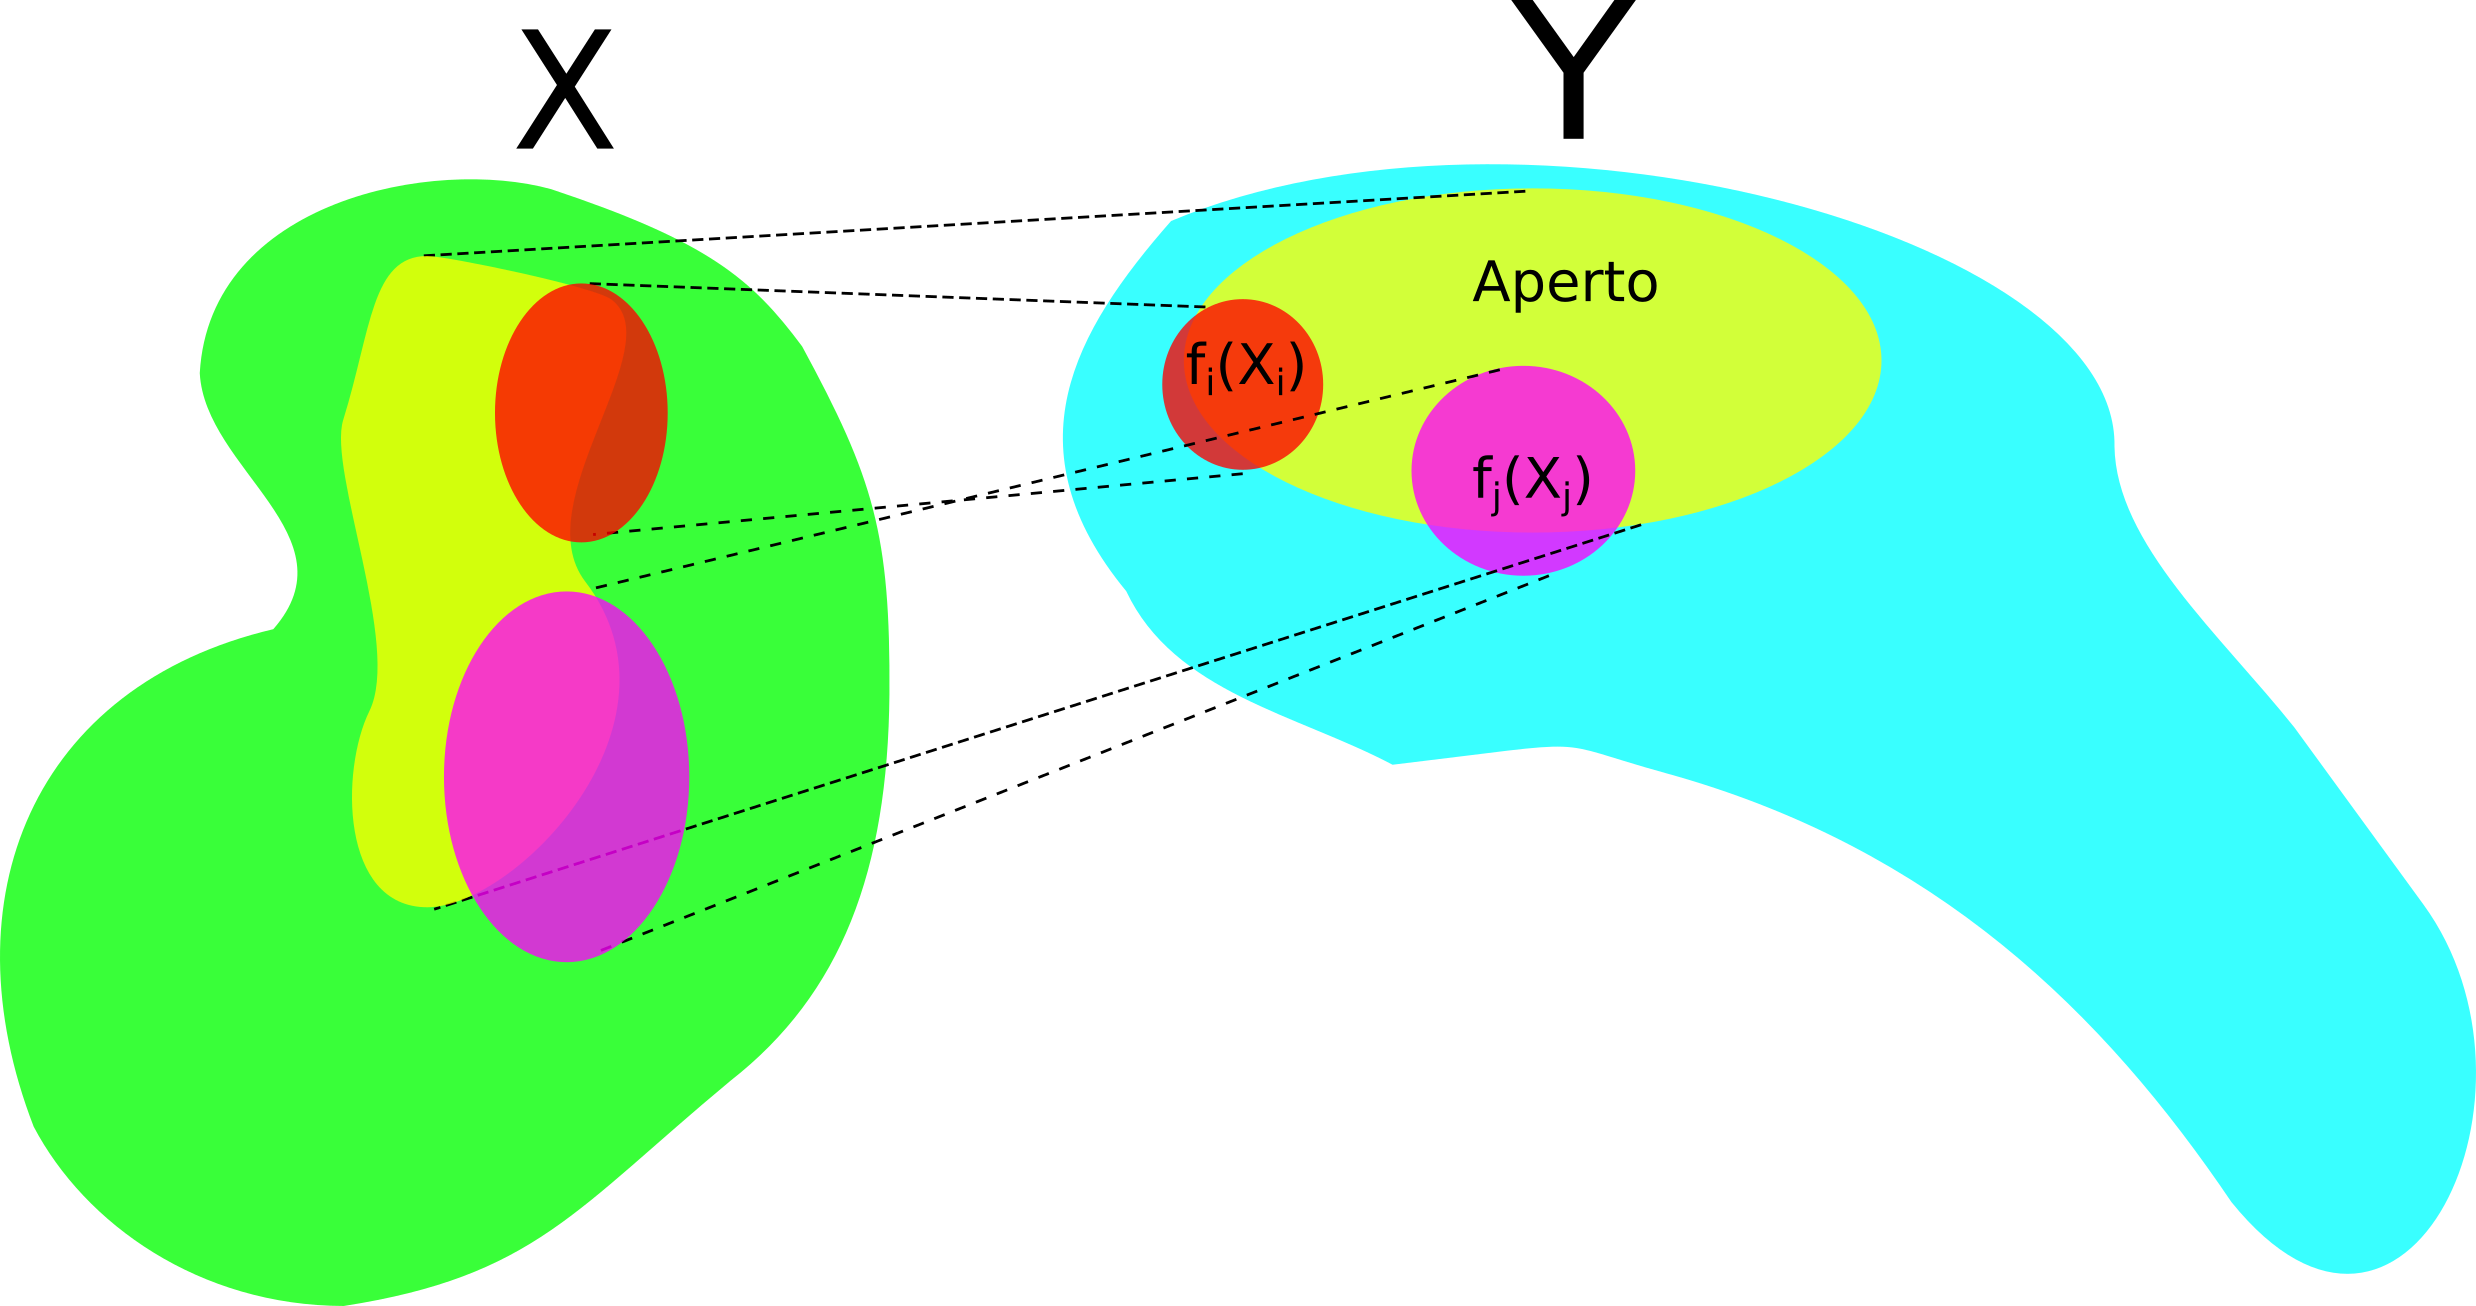
\includegraphics[width=0.6\linewidth]{images/topologia_generale/Coomology_exercises_figure}
		\caption{}
		\label{fig:coomologyexercisesfigure}
	\end{figure}

	Sia $A$ aperto in $\xi$. Allora considero $f^{-1}(A)$. Per la definizione di $f$ e siccome potrebbe essere che una parte di $A \cap \image{f_j} \neq \varnothing$ e $A \cap \image{f_i} \neq \varnothing$, allora prendo tutte quelle funzioni la cui immagine contiene punti di $A$. Allora vale 
	\begin{equation}
	\begin{aligned}
		f^{-1}(A) = \bigcup_{i} f_i^{-1}(A) 
	\end{aligned}
	\end{equation}
	ma poiché $f_i$ è continua in $X_i$, dev'essere che $f^{-1}(A) = X_i \cap A_i'$ dove $A' \in \tau$. Dunque 
	\begin{equation}
	\begin{aligned}
		f^{-1}(A) = \bigcup_{i} f_i^{-1}(A) = \bigcup_{i} X_i \cap A_i' 
	\end{aligned}
	\end{equation}
	ma $X_i, A'_i \in \tau$ quindi la loro intersezione è ancora un aperto, inoltre l'intersezione qualsiasi di aperti è un aperto. Segue che $f^{-1}(A)$ è aperto e dunque $f$ continua.
\end{proof}


\section{Prodotto di topologie}

In questa sezione si userà spesso la notazione $(X_1, \tau_1), (X_2, \tau_2), (X_1 \times X_2, \tau = \left\langle\tau_1 \times \tau_2 \right\rangle)$ per indicare tre spazi topologici. Quest'ultimo è il prodotto di due spazi topologici che adesso definiamo.

\begin{definition}
	La topologia $\tau$ che viene generata dalla base $\tau_1 \times \tau_2$ è detta topologia prodotto su $X_1 \times X_2$. Inoltre $(X_1 \times X_2, \tau)$ è uno spazio topologico e si dice prodotto degli spazi topologici $(X_1, \tau_1), (X_2, \tau_2)$.
\end{definition}

\begin{remark}
	Per quanto ovvio, facciamo vedere che $\tau_1 \times \tau_2$ forma una base su $X_1 \times X_2$. Per la Proposizione \ref{thr:sfi_generate_topology} un insieme è una base di $X_1 \times X_2$ se tale insieme copre $X_1 \times X_2$, ma questo è ovvio visto che $X_1 \times X_2 \in \tau_1 \times \tau_2$; e dati due elementi $A_1, A_2 \in \tau_1 \times \tau_2$ allora la loro intersezione $A_1 \cap A_2 = B_{1,1} \times B_{2,1} \cap B_{2,1} \times B_{2,2} = B_{1,1}\cap B_{2,1} \times B_{1,2} \cap B_{2,2}$ dove ogni $B_{j,i} \in \tau_j \cap A_i$ per cui sono ancora elementi di $\tau_1 \times \tau_2$. Pertanto è una base e identifica un unica topologia.
\end{remark}

\textbf{Esempio}

Si consideri $(\R^2, \tau^2_{\text{euclidea}})$, questo sarà omeomorfo a $(\R, \tau) \times (\R, \tau)$? Se la risposta fosse negativa non avrebbe senso parlare di prodotti di topologie, pertanto la risposta dev'essere affermativa. Vediamo perché:\\
% TODO: Aggiungere spiegazione


In generale quindi $\tau^n = \underset{n-volte}{\underbrace{\tau \times \dots \times \tau}}$ dove $\tau$ è la topologia euclidea. 

\begin{theorem}
	Sia $\mathcal{B}_1$ base di $\tau_1$ e $\mathcal{B_2}$ base di $\tau_2$, allora
	\begin{equation}
	\begin{aligned}	
		\mathcal{B}_1 \times \mathcal{B}_2 := \{B_1 \times B_2 \in 2^{\mathcal{B}_1 \times \mathcal{B}_2} \; | \; B_1 \in \mathcal{B}_1, \; B_2 \in \mathcal{B}_2\}
	\end{aligned}
	\end{equation}
	forma una base della topologia $\tau$ (ovvero il generato del prodotto delle topologie).
\end{theorem}
\begin{proof}
	Devo far vedere che se $A \in \tau$ allora è generato dalla base $\mathcal{B}_1 \times \mathcal{B}_2$. Allora se $A \in \tau$, la topologia è generata dalla base $\tau_1 \times \tau_2$. Per cui $A = \bigcup_{i \in I} A_{1,i} \times A_{2,i}$ dove $A_{1,i} \in \tau_1$ e $A_{2.i} \in \tau_2$ per ogni $i \in I$. Ma ogni $A_{1, i} = \bigcup_{B \in \mathcal{B}_{1,i}'} B$ dove $\mathcal{B}_{1,i}' \subset \mathcal{B}_1$ e analogamente per $A_{2,i}$. Sostituendo si ottiene
	\begin{equation}
	\begin{aligned}
		A = \bigcup_{i \in I} A_{1,i} \times A_{2,i} = \bigcup_{i \in I} \bigcup_{B \in \mathcal{B}_{1,i}'} B \times \bigcup_{B \in \mathcal{B}_{2,i}'} B = \bigcup_{\substack{i \in I \\ B_1 \in \mathcal{B}'_{1,i} \\ B_2 \in \mathcal{B}'_{2,i}}} B_1 \times B_2
	\end{aligned}
	\end{equation}
	Notare che $B_1 \times B_2$ indica tutti i possibili prodotti tra gli insiemi nelle rispettive famiglie, $\mathcal{B}'_{1,i}$ e $\mathcal{B}'_{2,i}$, e questi sono sempre elementi di $\mathcal{B}_1 \times \mathcal{B}_2$ e la somma dipende solo da $I$, per cui genera $A$. \\
	
	Devo vedere anche che la topologia generata da $\mathcal{B}_1 \times \mathcal{B}_2$ non sia più fine di $\tau$. Per cui sia $A \in \left\langle \mathcal{B}_1 \times \mathcal{B}_2 \right\rangle$. Allora $A = \bigcup_{i \in I} B_{1,i} \times B_{2,i}$, mi basta considerare la proiezione di $A$ (che è una mappa aperta) per vedere che $\pi_1(A) = \bigcup_{i \in I} B_{1,i} = A_1 \in \tau_1$ e analogamente per $\tau_2$. Per cui risulta che $A_1 \times A_2 = \pi_1(A) \times \pi_2(A) = A$.
\end{proof}


\begin{theorem}
	La topologia prodotto $\tau$ è la meno fine per cui le mappe $\morphism{\pi_i}{X_1\times X_2}{X_i}$ sono continue.
\end{theorem}
\begin{proof}
	Suppongo esista una topologia meno fine di $\tau$ che chiamerò $\tau'$. Allora $\pi_1$ è continua e quindi contine almeno tutti gli aperti della forma $\pi^{-1}_1(A_1) \times \pi^{-1}_2(A_2)$ dove $A_i$ aperto in $\tau_i$. Ma questi aperti sono esattamente gli aperti della base che generano $\tau$, pertanto $\tau \subset \tau'$.
\end{proof}

\begin{theorem}
	Le mappe $\morphism{\pi_i}{X_1\times X_2}{X_i}$ sono aperte (dove $i \in \{1,2\}$). 
\end{theorem}
\begin{proof}
	Si consideri $\pi_1(A)$ dove $A \in \tau$. Allora $A = \bigcup_{i \in I} A_{1,i} \times A_{2,i}$, per cui $\pi(A) = \pi(\bigcup_{i \in I} A_{1,i} \times A_{2,i}) = \bigcup_{i\in I} \pi_1 (A_{1,i} \times A_{2,i}) = \bigcup_{i \in I} A_{1,i}$. Poiché ogni $A_{1,i} \in \tau_1$ segue che anche la loro unione lo è. Analogamente si dimostra per la proiezione $\pi_2$.
\end{proof}

\begin{theorem}
	Siano $S_1 \subset X_1, S_2, \subset X_2$ allora il prodotto di sottotopologie si comporta bene, ovvero
	\begin{equation}
	\begin{aligned}
		\left\langle \tau_1 \times \tau_2 \right\rangle|_{S_1 \times S_2} = \left\langle \tau_1|_{S_1} \times \tau_2|_{S_2} \right\rangle 
	\end{aligned}
	\end{equation}
\end{theorem}
\begin{proof}
	Spezzo la dimostrazione nelle due inclusioni. Dimostro come primo caso $	\left\langle \tau_1 \times \tau_2 \right\rangle|_{S_1 \times S_2} \subset \left\langle \tau_1|_{S_1} \times \tau_2|_{S_2} \right\rangle$. Quindi sia $A \in \left\langle \tau_1 \times \tau_2 \right\rangle|_{S_1 \times S_2}$ allora $A = \left( \bigcup_{i \in I} A_{1,i} \times A_{2,i} \right) \cap S_1 \times S_2$, per cui posso distribuire l'intersezione su tutti gli elementi dell'unione:
	\begin{equation}
	\begin{aligned}
		\left( \bigcup_{i \in I} A_{1,i} \times A_{2,i} \right) \cap S_1 \times S_2 = \bigcup_{i \in I} (A_{1,i} \cap S_1) \times (A_{2,i} \cap S_2)
	\end{aligned}
	\end{equation}
	per il Teorema \ref{thr:proprieties_induced_top} per ogni $i \in I$, $(A_{1,i} \cap S_1) \times (A_{2,i} \cap S_2) \in \tau_1|_{S_1} \times \tau_2|_{S_2}$, ovvero $A \in \left\langle \tau_1|_{S_1} \times \tau_2|_{S_2} \right\rangle$. Come si può notare le implicazioni fatte sopra valgono anche nel verso opposto, per cui è dimostrata la tesi.
\end{proof}

\begin{theorem}
	Gli intorni si comportano bene rispetto al prodotto topologico. In particolare
	\begin{enumerate}
		\item Sia $(x_1, x_2) \in X_1\times X_2$. Allora $P \in \mathcal{N}_\tau((x_1,x_2))$ se e solo se esitono $U_1 \in \mathcal{N}_{\tau_1}(x_1)$ e $U_2 \in \mathcal{N}_{\tau_2}(x_2)$ tali che $U_1\times U_2 \subset P$.
		\item Sia $(x_1, x_2) \in X_1\times X_2$, $\mathcal{V}_1(x_1)$ e $\mathcal{V}_2(x_2)$ rispettivamente un sistema fondamentale di intorni di $x_1$ in $\tau_1$ e di $x_2$ in $\tau_2$. Allora $\mathcal{V}_1(x_1) \times \mathcal{V}_2(x_2)$ è un sistema fondamentale di intorni di $(x_1, x_2)$ nella topologia $\tau = \left\langle \tau_1 \times \tau_2 \right\rangle$.
	\end{enumerate}	
\end{theorem}
\begin{proof}[Punto 1]
	\begin{enumerate}
		\item[$\Leftarrow$] Abbastanza ovvio. Per definizion di intorno su $U_1$, allora esiste $A_1 \in \tau_1$ tale che $A_1 \subset U_1$ e analogo discorso su $\tau_2$. Per cui $A_1 \times A_2 \in \tau$ per definizione, inoltre ho che 
		\begin{equation}
		\begin{aligned}
			A_1 \times A_2 \subset U_1 \times U_2 \subset P
		\end{aligned}
		\end{equation}
		per cui $P$ è un intorno in $\tau$.
		\item[$\Rightarrow$] Per definizione di intorno vuol dire che esiste $A \subset P$ tale che $A \in \tau$. Allora $A = \bigcup_{i \in I} A_{1,i} \times A_{2,i}$, prendo $A_{1,i_0}, A_{2,i_0}$ tali da contenere rispettivamente $x_1, x_2$. Devo dimostrare che $A_{1,i_0}$ è un intorno di $x_1$ in $\tau_1$, ma è ovvio poiché $A_{1,i_0} \in \tau_1$. Analogo discorso su $A_{2,i_0}$. Ho dunque trovato un intorno in $\tau_1$ e uno in $\tau_2$ tali che il loro prodotto sta in $P$ (poiché il loro prodotto sta addirittura in $A \subset P$).
	\end{enumerate}
\end{proof}
\begin{proof}[Punto 2]
	% TODO
	\end{proof}

\begin{theorem}
	Siano $S_1 \subset X_1, S_2 \subset X_2$, allora valgono le seguenti formule
	\begin{equation}
	\begin{aligned}
		\overline{S_1\times S_2}^{\tau} & = \overline{S_1}^{\tau_1} \times \overline{S_2}^{\tau_2} \\
		Int(S_1 \times S_2) & = Int(S_1) \times Int(S_2)\\
		Fr(S_1 \times S_2) &= (Fr(S_1) \times \overline{S_2}) \cup (\overline{S_1} \times Fr(S_2))
	\end{aligned}
	\end{equation}
\end{theorem}
\begin{proof}[Dimostrazione equazione 1]
	Uso il fatto che un punto $x \in \overline{S_1\times S_2}^\tau$ se e solo se $x$ è aderente a $S_1 \times S_2$ in $\tau$. Fisso dunque un $(x_1, x_2) \in \overline{S_1\times S_2}^\tau$ e dei sistemi fondamentali di intorni $\mathcal{V}_{\tau_1}(x_1), \mathcal{V}_{\tau_2}(x_2)$.\\
	L'aderenza per definizione vuol dire che esiste un sistema fondamentale di intorni $\mathcal{V}_\tau(x) = \mathcal{V}_{\tau_1}(x_1) \times \mathcal{V}_{\tau_2}(x_2)$ tale che per ogni $V \in \mathcal{V}_\tau(x)$ vale $V \cap S_1 \times S_2 \neq \varnothing$. Usando la definizione data di $\mathcal{V}_\tau(x)$ posso riscrivere come per ogni $V_1 \in \mathcal{V}_{\tau_1}(x_1), V_2 \in \mathcal{V}_{\tau_2}(x_2)$ tali che $V_1 \times V_2 \cap S_1 \times S_2 \neq \varnothing$. \\
	Applicando un po' di leggi insiemistiche diventa $V_1 \cap S_1 \times V_2 \cap S_2 \neq \varnothing$, ovvero $V_1 \cap S_1 \neq \varnothing$ e $V_2 \cap S_2\neq \varnothing$ per cui dev'essere che $x_1$ sia aderente a $S_1$ secondo $\tau_1$ e analogamente per $x_2$. Per cui vale l'equazione. 
\end{proof}
\begin{proof}[Dimostrazione equazione 2]
	% TODO
\end{proof}
\begin{proof}[Dimostrazione equazione 3]
	Considero, analogamente a quanto fatto per dimostrare la prima equazione, posso prendere $(x_1,x_2) \in Fr(S_1 \times S_2)$. Fisso un sistema fondamentale di intorni su $S_1$ e $S_2$. Per cui se $x \in Fr(S_1 \times S_2)$ allora $V \cap S_1 \times S_2\neq \varnothing$ e $V \not\subset S_1 \times S_2$. Sostituendo la decomposizione per sistemi fondamentali di intorni $V_1 \times V_2 \cap S_1 \times S_2 = V_1 \cap V_2 \times S_1 \cap S_2\neq \varnothing$ per cui $V_1 \cap S_1 \neq \varnothing$ e $V_2 \cap S_2 \neq \varnothing$. Inoltre dalla condizione $V \not\subset S_1 \times S_2$ si ottiene le tre condizione $V_1 \subset S_1 \land V_2 \not\subset S_2$ o $V_1 \not\subset S_1 \land V_2 \subset S_2$ o $V_1 \not\subset S_1 \land V_2 \not\subset S_2$. Unendo tutte le condizioni si ottiene la tesi. 
\end{proof}

\begin{theorem}[Proprientà universale del prodotto topologico]
	\begin{equation}
		\begin{tikzcd}[column sep=0.7em]
		& (Y, \xi) \arrow[swap]{d}{f} \arrow[swap]{ddl}{f_1} \arrow{ddr}{f_2} & \\
		& (X_1 \times X_2, \tau) \arrow[swap]{dr}{\pi_2} \arrow{dl}{\pi_1} & \\
		(X_1, \tau_1) &  & (X_2, \tau_2)\\
		\end{tikzcd}
	\end{equation}
	Sia $\morphism{f}{(Y, \xi)}{(X_1 \times X_2, \tau)}$ una applicazione su spazi topologici e siano $\pi_1,\pi_2$ le proiezioni canoniche dal prodotto topologico. Allora $f_i = \pi_i \circ f$ si dicono componenti di $f$ e vale l'equivalenza delle seguenti affermazioni:
	\begin{enumerate}
		\item $f$ è continua;
		\item $f_i$ sono continue per $i \in \{1,2\}$.
	\end{enumerate}
\end{theorem}
\begin{proof}[Dimostrazione 1]
	\begin{enumerate}
		\item[$\Leftarrow$] Se $f$ continua allora $\pi_1 \circ f$ è continua perché composizione di funzioni continue, analogamente per $\pi_2 \circ f$.
		\item[$\Rightarrow$] Se le componenti $f_1, f_2$ sono continue. Allora si prenda un aperto $A \in \tau$, e si prenda la sua controimmagine attraverso $f$. È ovvio che 
		\begin{equation}
		\begin{aligned}
			f^{-1}(A) = f^{-1}(\bigcup_{i \in I} A_{1,i} \times A_{2,i}) = \bigcup_{i \in I} f^{-1}(A_{1,i} \times A_{2,i})
		\end{aligned}
		\end{equation}
		dove $A_{1,i}, A_{2,i}$ sono aperti rispettivamente in $\tau_1, \tau_2$. Siccome non abbiamo ancora usato l'ipotesi, è arrivato il momento di usarla. Infatti si vede che $f^{-1}_1(A_{1,i}) \cap f^{-1}_2(A_{2,i}) = f^{-1}(A_{1,i} \times A_{2,i})$, ma essendo $f_1, f_2$ continue, la loro controimmagine di aperti è aperta. Da cui ho anche $f^{-1}(A_{1,i} \times A_{2,i})$ aperto. Per cui $f$ è continua. 
	\end{enumerate}
\end{proof}
\begin{proof}[Dimostrazione utilizzando le proprietà degli s.f.i.]
	% TODO
\end{proof}

\begin{theorem}
	Sia $\morphism{g}{(X_1 \times X_2, \tau)}{(Y, \xi)}$. Fissato un $(x_1, x_2) \in X_1 \times X_2$. Allora posso dire che $g$ è continua in $(x_1, x_2)$ se per ogni $U \in \mathcal{N}_\xi(g(x_1,x_2)))$ esistono $V_1 \in \mathcal{V}_1(x_1)$ e $V_2 \in \mathcal{V}_2(x_2)$ tali che $g(V_1 \times V_2) \subset U$.
\end{theorem}
\begin{proof}
	Se $g$ è continua in $x$ allora per ogni intorno $V$ di $g(x)$ esisterà un intorno $N$ di $x$ tale che $g(N) \subset V$. Poiché $N$ è un intorno nella topologia prodotto allora esistono $N_1, N_2$ rispettivamente intorni di $x_1, x_2$ dove $x = (x_1, x_2)$. Ovvero la tesi.\\
	Al contrario fissiamo un $V$ intorno di $g(x)$, allora devo dimostrare che $g^{-1}(V)$ è ancora un intorno di $x$, ma questo è ovvio dato che esistono $N_1, N_2$ tali che $g(N_1 \times N_2) \subset g(g^{-1}(V)) \subset V$ e quindi $N_1 \times N_2 \subset g^{-1}(V)$. 
\end{proof}

Notare che in generale i teoremi dimostrati per $n=2$, ovvero $X_1 \times X_2$, valgono anche per $n \in \N$, infatti basta procedere per induzione. Il vero problema è dimostrare che $X_1 \times X_2 \times \dots \times X_n \simeq X_1 \times (X_2 \times \dots \times X_n)$ e così via. Ovvero dimostrare che il prodotto di topologie è un operatore associativo nella categoria degli spazi topologici. 

\begin{theorem}
	Le topologie con il prodotto formano un monoide commutativo su $\mathbb{Top}/\sim$ dove $X\sim Y$ se e solo se $X$ è omeomorfo $Y$.
\end{theorem}
\begin{proof}
	\begin{enumerate}
		\item Associatività. 
		\item Commutatività. Basta definire la mappa $\morphism{f}{X\times Y}{Y \times X}$, con $f(x,y) = (y,x)$. La mappa così definita è continua, biettiva e aperta. Per cui la commutatività vale.
		\item L'identita è il singoletto $\{p\}$ con la topologia qualsiasi (tanto è sempre la solita). Quindi sia $(X, \tau)$ uno spazio topologico. Definisco la mappa $\morphism{f}{(X, \tau)}{(X\times \{p\}, \tau'}$ definibile nell'unico modo possibile. La mappa è biettiva perché $f^{-1}(x, p) = x$ è la sua funzione inversa. È ovviamente continua perché $f^{-1}((A, \varnothing)) = \varnothing$, $f^{-1}((A, \{p\})= A$ perché $f$ biettiva. E analogamente si dimostra che è aperta. Pertanto è l'identità. 
	\end{enumerate}
\end{proof}

\section{Topologie quozienti}

\begin{definition}[Topologia quoziente]
	Sia $(X, \tau)$ spazio topologico e $\morphism{f}{X}{Y}$ applicazione, con $Y \neq \varnothing$. Si dice topologia quoziente su $Y$ rispetto ad $f$, oppure topologia indotta da $f$ su $Y$, la più fine topologia su $Y$ tale che $f$ è continua. 
\end{definition}

\begin{theorem}
	Sia $(X, \tau)$ spazio topologico e $\morphism{f}{X}{Y}$ applicazione e $Y \neq \varnothing$. Valgono le seguenti affermazioni 
	\begin{enumerate}
		\item La topologia quoziente su $Y$ rispetto a $f$ esiste ed è unica, denotandola come $\tau_f$ vale 
		\begin{equation}
		\tau_f := \left\{ A \in 2^Y \; | 
		\; f^{-1}(A) \right\}
		\end{equation}
		\item $C$ è chiuso in $\tau_f$ se e solo se $f^{-1}(C)$ è chiuso in $\tau$.
		\item \textbf{Proprietà universale degli  spazi quozienti} 
		\begin{equation}
		\begin{tikzcd}
		(X, \tau) \arrow[swap]{rd}{g\circ f} \arrow{r}{f} & (Y, \tau_f) \arrow{d}{g} \\
		& (Z, \mu) 
		\end{tikzcd}
		\end{equation}
		$g$ è continua se e solo se $g \circ f$ è continua. 
	\end{enumerate}
\end{theorem}
\begin{proof}
	\begin{enumerate}
		\item È ovviamente una topologia ed è la più fine. 
		\item La controimmagine commuta con il complementare. 
		\item Se $g$ è continua è ovvio che $g \circ f$ è continua perché la composizione di funzioni continue è continua. Se $f\circ g$ è continua allora se $g$ continua allora $g^{-1}(A)$ è un aperto. Ma $ \tau_f \ni g^{-1}(A) \Leftrightarrow f^{-1}g^{-1}(A) \in \tau$ ma l'ultima è banalmente ovvia visto che $g \circ f$ continua. \footnote{Perché è interessante questa proprietà universale? Innanzitutto perché è universale su tutte le topologie quozienti, secondariamente perché ti permette di by-passare la topologia quoziente per trovare che una mappa è continua, senza dover lavorare sulla topologia quoziente stessa.}
	\end{enumerate}
\end{proof}

\begin{remark}
	sia $\morphism{f}{(X, \tau)}{Y, \tau_f)}$ se $f$ non surgettiva allora $\exists y \in Y \setminus f(X)$, il singoletto $\{y\}$ è un aperto nella topologia $\tau_f$ poiché $f^{-1}(y) = \varnothing$.
\end{remark} 

\begin{definition}
	Sia $\morphism{f}{X}{Y}$ applicazione e sia $S \subset X$. Diciamo che $S$ è \textbf{saturo}\footnote{Un'idea del termine è che essenzialmente la funzione \textit{divora} tutte le fibre di $S$ in modo tale che stiano in $S$ stesso, infatti se ho una saturazione ho la stessa cosa} rispetto a $f$, se $f^{-1}(f(S)) = S$.
\end{definition} 

\begin{remark}
	$S$ è saturo in $f$.
	\begin{equation}
	S = f^{-1}f(S) = \bigcup_{x \in S} f^{-1}f(x)
	\end{equation}
	ovvero se per ogni $x \in S$ abbiamo una unica fibra in $S$. Ovvero $S$ contiene tutte le fibre contenenti i suoi punti. 
\end{remark} 

\begin{remark}
	Se $f$ iniettiva allora ogni insieme è $f$-saturo, poiché $S = f^{-1}f(S)$.
\end{remark}

\begin{theorem}
	$\morphism{f}{X}{Y}$ applicazione e sia $S \subset X$. $f^{-1}f(S)$ si dice \textbf{$f$-saturazione} di $S$. Si può dimostrare che 
	\begin{enumerate}
		\item $S \subset f^{-1}f(S)$
		\item $f^{-1}f(S)$ è il più piccolo insieme $f$-saturo contenente $S$.
	\end{enumerate}
\end{theorem}
\begin{proof}
	\begin{enumerate}
		\item Ovvio. Volendo usare quanto detto nell'osservazione precedente
		\begin{equation}
		\begin{aligned}
			S = \bigcup_{x\in S} \{x\} \subset \bigcup_{x \in S} f^{-1}f(x)
		\end{aligned}
		\end{equation}
		\item È semplice vedere che
		\begin{equation}
		\begin{aligned}
			f(f^{-1}(f(S))) = f(S) \Longrightarrow f^{-1}(f(f^{-1}(f(S)))) = f^{-1}(f(S))
		\end{aligned}
		\end{equation}
		poiché se $x \in f^{-1}(f(S))$ allora $f(x) \in f(S)$ per definizione (e viceversa), quindi la $f$-saturazione di $S$ è $f$-satura. Devo inoltre dimostrare che è la più piccola. Per cui sia $K$ $f$-saturo tale che $S \subset K \subset f^{-1}f(S)$. Allora applicando $f^{-1}f$ sulla precedente successione di inclusioni
		\begin{equation}
		\begin{aligned}
			f^{-1}f(S) \subset f^{-1}f(K) \overset{\text{è f-sat.}}{=} K \subset f^{-1}ff^{-1}f(S) = f^{-1}f(S) 
		\end{aligned}
		\end{equation}
		per cui dev'essere che $K = f^{-1}f(S)$. Per cui la più piccola è per forza $f^{-1}f(S)$ 
	\end{enumerate}
\end{proof}


\section{Quozienti con mappe surgettive}

Poiché la topologia quoziente è difficile da studiare da sola, quindi si  cerca di collegare le proprietà della topologia $\tau_f$ a quella di partenza $\tau$.

\begin{lemma}
	$\morphism{f}{X}{Y}$ applicazione surgettiva e $S \subset X$ $f$-saturo, allora 
	\begin{enumerate}
		\item $S^c$ è $f$-saturo 
		\item $f(S^c) = f(S)^c$
	\end{enumerate}
\end{lemma}
\begin{proof}
	Dimostro per prima cosa $f(S)^c = f(S^c)$. Data $f$ suriettiva allora 
	\begin{equation}
	f(X) = f(S \cup S^c) = f(S) \cup f(S^c) = Y
	\end{equation}
	e dunque $f(S^c) = Y \setminus f(S) = f(S)^c$. 
	Per la $f$-saturazione di $S$ ho che $S = f^{-1}f(S)$, dunque applicando il complementare ho che $S^c = f^{-1}(f(S))^c = f^{-1}(f(S)^c) = f^{-1}(f(S^c))$
\end{proof}

\begin{theorem}
	Sia $(X, \tau)$ spazio topologico e $\morphism{f}{X}{Y}$ surgettiva e dato $Y$ con $\tau_f$ allora vale 
	\begin{enumerate}
		\item $A \subset Y$ è un aperto in $\tau_f$ se e solo se esiste $Q \in \tau$ tale da essere $f$-saturo e che $f(Q) = A$. Dunque vale 
		\begin{equation}
		\tau_f = \mathcal{A} = \{ A \in 2^Y \;|\; A = f(S), \text{dove} \; S \in \tau, f^{-1}f(S) = S\}
		\end{equation}
		\item $C \subset Y$ è un chiuso in $\tau_f$ se e solo se esiste $Q \subset X$ chiuso tale da essere $f$-saturo e che $f(Q) = C$.
	\end{enumerate}
\end{theorem}
\begin{proof}
	\begin{enumerate}
			\item Sia $A \in \mathcal{A}$ allora esiste $S \in \tau$ tale da essere $f$-saturo. Per cui $f^{-1}(A) = f^{-1}(f(S)) \overset{\text{saturazione}}{=} S \in \tau$. Questo dimostra $\mathcal{A} \subset \tau_f$. Sia dunque $A \in \tau_f$ e $U = f^{-1}(A) \in \tau$ devo dimostrare che $U$ è $f$-saturo. 
			Dato che $f(f^{-1}(A)) = A$ per la surgettività di $f$   
			\begin{equation}
			\begin{aligned}
				f^{-1}f(U) = f^{-1}(A) = U
			\end{aligned}
			\end{equation} 
			e dunque è anche $f$-saturo. Si evince che $\tau_f \subset \mathcal{A}$ e dunque anche che $\tau_f = \mathcal{A}$.
		\item Devo dimostrare che un chiuso in $\tau_f$ è sempre della forma $K = f(C)$ per $C$ $f$-saturo e $C$ chiuso in $\tau$. Quindi vale che $K^c = f(S)$ dove $S \in \tau$ e $f$-saturo. Quindi posso riscrivere $S = C^c$ dove $C$ chiuso in $\tau$. Per il precedente lemma ho dunque
		\begin{equation}
		\begin{aligned}
			K^c = f(S) = f(C^c) \overset{\text{lem. prec.}}{=} f(C)^c
		\end{aligned}
		\end{equation}
		dove $C$ è un chiuso $f$-saturo. Ovvero per ogni $K$ chiuso in $\tau_f$, vale $K = f(C)$ per qualche $C$ chiuso in $\tau$ e $f$-saturo (e viceversa), cioè la tesi.
	\end{enumerate}
\end{proof}

\begin{definition}
	Una applicazione $\morphism{f}{(X,\tau)}{(Y, \xi)}$ tra spazi topologici è detta \textbf{identificazione} se $f$ è continua, surgettiva e $\xi = \tau_f$.
\end{definition}

\begin{theorem}[Caratterizzazione delle indentificazioni]
	\label{crtident}
	Sia $\morphism{f}{(X,\tau)}{(Y, \xi)}$ applicazione continua e surgettiva, allora le seguenti affermazioni sono equivalenti
	\begin{enumerate}
		\item $f$ è un identificazione
		\item Se $\forall A \subset Y$  tale che $f^{-1}(A) \in \tau$ allora $A \in \xi$
		\item Se $\forall A \in \tau$, $A$ è $f$-saturo e $f(A) \in \xi$.
		\item Se $\forall C \subset X$ chiuso e $f$-saturo vale $f(C)$ chiuso in $\xi$
	\end{enumerate}
\end{theorem}
\begin{proof}
	\begin{enumerate}
		\item[$1 \Leftrightarrow 2$] $f$ identificazione se e solo se $\tau_f = \xi$ e abbiamo gratis che $\xi \subset \tau_f$ perché topologia più fine tale da render $f$ continua. Quindi bisogna dimostrare $\tau_f \subset \xi \Longleftrightarrow \forall A \subset Y$ tali che $f^{-1}(A) \in \tau \Rightarrow A \in \xi$. Per cui se vale $\tau_f \subset \xi$ è ovvio che ogni $A$ $f^{-1}(A) \in \tau$ allora $A \in \tau_f \subset \xi$ e ho la tesi. Se invece vale $\forall A \subset Y$ tali che $f^{-1}(A) \in \tau \Rightarrow A \in \xi$ allora se prendo $A \in \tau_f$ allora dev'essere che $f^{-1}(A) \in \tau$ e per ipotesi vale anche che $A \in \xi$ quindi $\tau_f \subset \xi$. 
		\item[$1 \Rightarrow 3$] Fisso $U \in \tau$ tale da essere $f$-saturo, allora $f(U) \in \xi = \tau_f$, ma $\xi = \tau_f$ per ipotesi, ovvero si ottiene la tesi.
		\item[$3 \Rightarrow 1$] Se vale $f(U) \in \xi$ devo provare che $\xi = \tau_f$, ma $\xi \subset \tau_f$ è già dimostrata poiché $\tau_f$ è la topologia più fine per cui $f$ sia continua. Per cui fisso un $A \in \tau_f$. $A \in \tau_f \Leftrightarrow \exists U \in \tau$ e $f$-saturo, ma per ipotesi $f(U) \in \xi$, quindi $\tau_f \subset \xi \subset \tau_f$.
		\item[$3\Leftrightarrow 4$] Ovvio per teoremi precedenti.
	\end{enumerate}
\end{proof}


\begin{remark}
	Notare che le identificazioni nono sono sempre applicazioni aperte, anche se sono aperte e chiuse rispetto a una classe di insiemi (ovvero quelli $f$-saturi). Infatti possiamo definire una applicazione non aperta e non chiusa che chiamiamo $f$. Allora $\morphism{f}{(\R, \tau_{\text{euclidea}})}{(\{0,1\})}$, con $f := \mathcal{X}_{\left[0,2\right)}$ dove la $\mathcal{X}$ è la mappa caratteristica dell'insieme a pedice. È ovvio che $\tau_f$ in questo caso è la topologia banale, infatti $0$ non può essere un aperto, in quanto se lo fosse $f^{-1}(0) = \left[0, 2\right)^c$ che non  è né aperto né chiuso. Analogamente per il punto $1$ che non può essere aperto (e neanche chiuso). Inoltre $f((0,2)) = 1$, per cui non manda aperti in aperti e analogamente si vede che $f(\left[0,1\right]) = 1$ e dunque non manda neanche chiusi in chiusi, eppure $f$ è una identificazione.
\end{remark}

\begin{theorem}
	Sia $\morphism{f}{(X,\tau)}{(Y, \tau_f)}$ identificazione allora valgono le seguenti affermazioni
	\begin{enumerate}
		\item $f$ aperta se e solo se $\forall A \in \tau$ la sua $f$-saturazione $f^{-1}f(A) \in \tau$
		\item $f$ chiusa se e solo se $\forall C$ chiuso la sua $f$-saturazione $f^{-1}f(C)$ è un chiuso.
	\end{enumerate}
\end{theorem}
\begin{proof}
	Dimostro solo il primo caso, il secondo è equivalente al primo dato quanto visto fin ora. Se $f$ aperta allora $\forall A \in \tau$ risulta che $f(A)$ è aperta per ipotesi e $f^{-1}f(A)$ dev'essere ancora un aperto perché $f$ continua. Se invece vale che la $f$-saturazione di un aperto è ancora aperta, fisso $A \in \tau$ e voglio vedere che $f(A)$ è un aperto in $\tau_f$. Ma $f(A) \in \tau_f$ se e solo se esiste $S \in \tau$ e $f$-saturo tale che $f(S) = f(A)$. Basta scegliere $S = f^{-1}f(A)$ e sappiamo che appartiene a $\tau$, è $f$-saturo e inoltre poiché $f$ suriettiva $f(S) = f(f^{-1}f(A)) = f(A)$. Pertanto $f$ è aperta. 
\end{proof}

\section{Relazioni di equivalenza e spazi quozienti}

Per creare uno spazio quoziente ci servono un paio di ingredienti
\begin{enumerate}
	\item Un insieme non vuoto, $X$.
	\item Una relazione di equivalenza $R \subset X \times X$.
\end{enumerate}

Una volta presi questi ingredienti è bene controllare le date di scadenza. Da qui in avanti diventa semplice, si quozientizza. Si prenda $X$ e lo si faccia diventare $X / R$ ovvero l'insieme delle classi di equivalenza di $X$ in $R$. 

\begin{figure}[h]
	\centering
	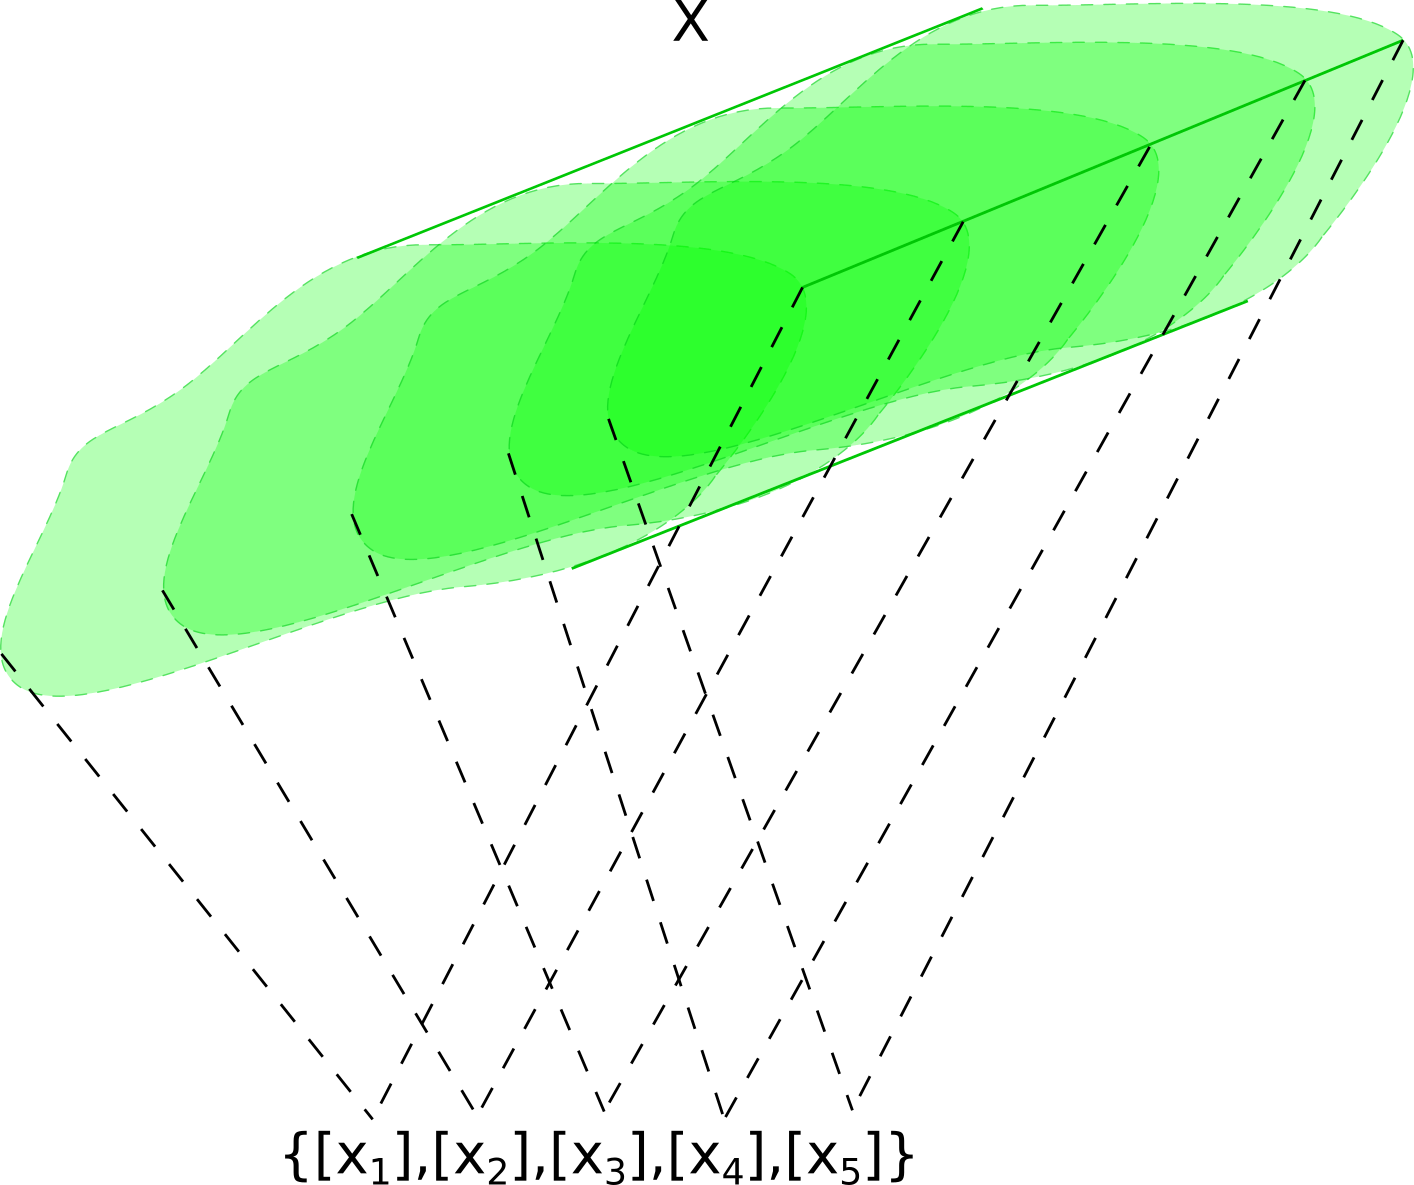
\includegraphics[width=0.5\linewidth]{images/topologia_generale/projection_quotient}
	\caption{Proiezione della partizione di $X$ data dalla relazione $R$. Oppure si possono vedere i sottoinsiemi verdi di $X$ come tutte le fibre di $f$ su un $X'$ e che vengono proiettate in un punto da $\pi$}
	\label{fig:projectionquotient}
\end{figure}

Dopo questo procedimento (circa 2-3 minuti) si può iniziare a operare sui morfismi e construire una mappa 
\begin{equation*}
\begin{tikzcd}[row sep = tiny]
	\pi  \colon &  X \arrow{r} & X/R \\
		 & x \arrow[mapsto]{r} & \left[x\right]_R
\end{tikzcd}
\end{equation*}


che è la \textbf{proiezione naturale} dell'insieme sul suo quoziente. Questa è sempre suriettiva (per questo si sono sempre studiate mappe suriettive nel capitolo precedente) e si comporta bene come si può vedere dalla figura. Utilizzando il procedimento canonico per la costruzione di topologie quozienti indotte da applicaizioni sulla proiezione naturale si ottiene quella che è detta \textbf{topologia quoziente di $\tau$ modulo $R$} e $(X/R, \tau_\pi)$ è detto lo spazio topologico quoziente di $(X,\tau)$ modulo $R$.

\begin{lemma}
	\label{lem_qdom}
	Sia $\morphism{f}{(X, \tau)}{(X', \tau')}$ applicazione continua tra spazi topologici e siano $R, R'$ relazioni di equivalenza rispettivamente su $X, X'$. Vale $f(\left[x\right]_R) \subset \left[f(x)\right]_{R'}$ (equivale alla condizione $xRy \Rightarrow f(x)R'f(y)$) se e solo se esiste ed è unica una $g$ continua tale che 
	\begin{equation}
	\begin{tikzcd}[row sep = 3em]
		(X, \tau) \arrow[swap]{d}{\pi} \arrow{r}{f} & (X', \tau') \arrow{d}{\pi'}\\
		(X/R, \tau_{X/R}) \arrow[swap]{r}{\exists! g} & (X'/R', \tau_{X'/R'})
	\end{tikzcd}
	\end{equation} 	
	il diagramma commuta.
\end{lemma}
\begin{proof}
	Se esiste $g$ per cui il diagramma commuta stiamo praticamente dicendo 
	\begin{equation}
	\begin{aligned}
		(\pi' \circ f)(x) = (g \circ \pi)(x) = (g \circ \pi)(y) = (\pi' \circ f)(y)
	\end{aligned}
	\end{equation}
	ma questa uguaglianza vale se e solo se $f(x) R' f(y)$, per cui ho la tesi.\\
	
	Dimostro l'esistenza di $g$ e la definisco come $g(\alpha) = (\pi' \circ f)(x_\alpha)$ dove $x_\alpha = \pi^{-1}\alpha$, ovvero $x_\alpha$ è un rappresentante della classe $\alpha$. Devo far vedere che sia ben definita, altrimenti non \textit{esiste}.
	Per cui considero anche un altro rappresentate della classe $\alpha$ e lo chiamo $x'_\alpha$. Affinché sia ben definita dev'essere che $g(\alpha) = \pi'f(x_\alpha) = \pi' f(x'_\alpha) = g(\alpha)$, ma questa condizione è vera per l'ipotesi. La continuità di $g$ è data dalla proprietà universale degli spazi quozienti, si consideri il seguente diagramma commutativo
	\begin{equation}
		\begin{tikzcd}[row sep = 3em]
			(X,\tau) \arrow{d}{\pi} \arrow{rd}{\pi' \circ f} & \\
			(X/R, \tau_{X/R}) \arrow{r}{g} & (X'/R', \tau_{X'/R'})
		\end{tikzcd}
	\end{equation}
	per cui $g$ è continua dato che $\pi' \circ f$ è continua.
\end{proof}

\begin{theorem}
	Sia  $\morphism{f}{X}{X'}$ una applicazione continua e surgettiva possiamo definire la relazione di equivalenza $R_f$ sull'insieme $X$ ponendo la relazione $xR_fy \Leftrightarrow f(x) = f(y)$. Allora 
	\begin{enumerate}
		\item esiste ed è unica $\morphism{g}{X/R_f}{X'}$ tale che $g$ biettiva e continua.
		\item $g$ è un omeomorfismo se e solo se $f$ è un identificazione.
	\end{enumerate}
\end{theorem}
\begin{proof}
	Basta applicare il Lemma \ref{lem_qdom} sul seguente diagramma
	\begin{equation}
	\begin{tikzcd}[row sep = 3em]
		(X, \tau) \arrow[swap]{d}{\pi} \arrow{r}{f} & (X', \tau') \arrow{d}{\pi' = \operatorname{Id}}\\
		(X/R_f, \tau_{X/R_f}) \arrow[swap]{r}{\exists! g} & (X'/U', \tau_{X'/U'}) = (X', \tau')
	\end{tikzcd}	
	\end{equation}
	dove la relazione $U'$ su $X'$ è definita come $xU'y \Leftrightarrow x = y$, per cui la proiezione $\pi'$ non è nient'altro che l'identità. Inoltre il diagramma
	\begin{equation}
	\begin{tikzcd}[row sep = 3em]
		(X, \tau) \arrow[swap]{d}{\pi} \arrow{r}{f} & (X', \tau') \\
		(X/R_f, \tau_{X/R_f}) \arrow[swap]{ru}{\exists! g} &
	\end{tikzcd}	
	\end{equation}
	commuta. 
	Per la commutatività del diagramma precedente si ottiene gratis che $f = g \circ \pi$ e quindi dev'essere che se $f$ è suriettiva anche $g$ lo è. Inoltre $g$ è anche iniettiva. Siano $\left[x\right] \neq \left[y\right]$ allora 
	\begin{equation}
	\begin{aligned}
		f \circ \pi^{-1} (\left[x\right]) = g(\left[x\right]) \neq g(\left[y\right]) = f \circ \pi^{-1}(\left[y\right])
	\end{aligned}
	\end{equation}	
	poiché ogni controimmagine di una classe $\pi^{-1}(\left[x\right])$ sono tutti quegli $x_i \in X$ tali che $f(x_1) = f(x_2) = \dots = f(x_i)$. Dunque è anche iniettiva e risulta essere biettiva.\\
	
	Dimostro il secondo punto del teorema, per cui separo i due casi
	\begin{enumerate}
		\item[$\Leftarrow$] Sia $f$ indentificazione. Notare che abbiamo già che $g$ contina e biettiva, ci manca da dimostrare che $g$ aperta.  Sia $A \in \tau_{X/R_f}$ allora $\pi^{-1}(A) \in \tau$ ed è $f$-saturo. Allora $f(\pi^{-1}(A)) \in \tau_f$ e poiché $f = g \circ \pi$ risulta 
		\begin{equation}
		\begin{aligned}	
			 \tau_f \ni f(\pi^{-1}(A)) = g ((\pi \circ \pi^{-1})(A)) = g(A)
		\end{aligned}
		\end{equation}
		quindi $g$ è aperta e un omeomorfismo.
		\item[$\Rightarrow$] Poniamo $g$ omeomorfismo. Dobbiamo dimostrare che $f$ è un identificazione, sappiamo già che $f$ suriettiva e continua, quindi dobbiamo dimostrare l'uguaglianza delle  topologie in arrivo. Per questo possiamo scegliere una delle caratterizzazioni date dal Teorema \ref{crtident}. In particolare se riusciamo a dimostrare che per ogni $A' \in 2^X$ tale che $f^{-1}(A') \in \tau$ allora $A' \in \tau'$ abbiamo vinto. Fisso un $A'$ tale che $f^{-1}(A') \in \tau$. Ma questo è $\pi$-saturo, quindi vale che $\pi f^{-1} (A') \in \tau_{X/R_f}$, inoltre grazie al fatto che $g$ è un omeomorfismo possiamo portare in avanti l'aperto senza problemi
		\begin{equation}
		\begin{aligned}
			\tau' \ni g\pi (f^{-1}(A')) = ff^{-1}(A') \overset{f \; \text{surg.}}{=} A' 
		\end{aligned}
		\end{equation}
		che è quanto si voleva dimostrare.
	\end{enumerate}
\end{proof}

I seguenti corollari sono praticamente simili e indicano la stessa cosa, ma in modi distinti e di diversa utilità pratica. 

\begin{corollary}
	Se $\morphism{f}{(X,\tau)}{(X',\tau')}$ è una identificazione allora $(X/R_f, \tau_{R_f}) \simeq (X', \tau')$. 
\end{corollary}

\begin{corollary}
	Sia $(X,\tau)$ spazio topologico e sia $R$ relazione di equivalenza su $X$ e sua $\morphism{\pi}{(X,\tau)}{(X/R, \tau_{X/R})}$ proiezione naturale e $(X', \tau')$ un altro spazio topologico. Supponiamo esista $\morphism{f}{(X,\tau)}{(X',\tau')}$ identificazione tale che $f^{-1}f(x) = \left[x\right]_R$ per ogni $x \in X$ allora $X/R \simeq X'$.
\end{corollary}

\section{Gruppi topologici}

\begin{definition}
	Sia $(X, \tau)$ uno spazio topologico con $\dot \colon X \times X \rightarrow X$ un operatore di gruppo su $X$. Allora è un gruppo topologico se $x \dot y^{-1}$ è una funzione continua.
\end{definition}

Alcuni esempi:
\begin{enumerate}
	\item $\R$ con la topologia euclidea e l'addizione è un gruppo topologico.
	\item $\Z, \Q$ sono due sottogruppi normale di $\R$ rispetto all'addizione. 
	\item $\operatorname{GL}_n$ e i suoi sottogruppi sono gruppi topologici.
\end{enumerate}

Questi sono interessanti perché si possono costruire i seguenti quozienti topologici:
\begin{theorem}
	$\R^n / \Z^n \simeq \S^n$
\end{theorem}
\begin{proof}
	Non credo di essere in grado per una completa dimostrazione, però nel caso $n=1$ e $n=2$ è abbastanza intuitiva.
	
	Sia $n=1$. Allora tutti gli elementi di $\R / \Z = \{a + \Z \; |\; a \in \left[0,1\right) \}$.  
	Per cui viene indentificato lo $0$ con $1$ quindi è la stessa cosa che si faceva per dimostrare che $\left[0,1\right]/ \sim \simeq \S$. 
\end{proof}
 
%todos: 8

\chapter{Proprietà topologiche}
Se esiste una categoria di proprietà che è fondamentale avere bene a mente in topologia, queste sono le proprietà topologiche. 
In sostanza diciamo \textbf{proprietà topologica} una caratteristica invariante per omeomorfismi; vedremo presto come applicarle allo studio della topologia generale che abbiamo appena completato.



\section{Proprietà di Hausdorff $T_2$}
\subsection{\textcolor{TopGener}{\textbf{La proprietà $T_2$}}}
 
 
 
\begin{definition}
	Sia $(X, \tau)$ spazio topologico, è detto \textbf{di Hausdorff} (o $T_2$) se $\forall \ x, y, x \neq y$ esistono due intorni $U, V \in \mathcal{N}_\tau(x),\mathcal{N}_\tau(y)$ tali che $U \cap V = \varnothing$.
\end{definition} 


La proprietà di Hausdorff è detta $T_2$,  esistono anche $T_0, T_1, T_3, T_4$, altre proprietà più deboli o più forti (a seconda della loro numerazione) di quella di Hausdorff. \\ La più forte, $T_4$, richiede che in due insiemi chiusi disgiunti ogni intorno dei loro punti sia disgiunto e viene anche detta \textbf{normalità}. La più debole, $T_1$, richiede che i sottoinsiemi singoletti di $X$ siano chiusi.\\ \\ Esistono interessanti relazioni tra le varie proprietà $T_i$, ad esempio $T_2$ implica $T_1$ ma l'inverso non vale. \footnote{si veda un insieme $X$ infinito con topologia cofinita, è immediato verificare che vale come controesempio.}

\begin{remark}
	La condizione di Hausdorff è topologica. \\  Infatti è preservata dagli omeomorfismi:
	\begin{center}
		$(X,\tau)$ è di Hausdorff se e solo se anche $(Y,\xi)$ è di Hausdorff ed esiste $\morphism{f}{(X,\tau)}{(Y,\xi)}$ omeomorfismo tra i due spazi topologici
	\end{center}
	 Se $x,y \in X$ e $x\neq y$, allora $f(x), f(y) \in Y$ e $f(x) \neq f(y)$ poiché $f$ biettiva. Se esistono degli $U,V\in \mathcal{N}_\tau(x),\mathcal{N}_\tau(y)$ tali che $U \cap V = \varnothing$, esistono $A \subset U$ e $A' \subset V$ aperti tali che $A \cap A' = \varnothing$. Per cui $f(A) \cap f(A') = \varnothing$, dove $f(A), f(A')$ sono aperti ed intorni rispettivamente di $f(x),f(y)$. Quindi la proprietà vale. Inoltre applicando l'inversa si ottiene l'altra implicazione.
\end{remark} 
\begin{remark}
	Se $(X, \tau)$ è di Hausdorff, allora ogni topologia più fine $\tau \subset \xi$ è di Hausdorff su $X$. \\ Infatti a noi interessano soltanto gli aperti \textit{più piccoli} e non quelli più grossi. Se ci sono aperti più piccoli e sappiamo che ce ne sono già di piccoli abbastanza affinché sia Hausdorff, non danno problema. Se ci sono aperti più grossi, non è interessante comunque, perché per la proprietà di Hausdorff ci servono solamente degli aperti \enquote{abbastanza piccoli}. \\ \\ Se si volesse proprio fare una dimostrazione: sia $x \neq y$ allora $\tau \subset \xi$ per cui esistono in $\tau$ $U \cap V = \varnothing$ e quindi $U, V$ sono ancora intorni in $\xi$, pertanto anche $\xi$ è di Hausdorff. 
\end{remark}
\begin{remark}
	Sia $(X, \tau)$ spazio topologico, se per ogni $A, B\in \tau$ si ha che $A\cap B \neq \varnothing$ allora $\tau$ non è di Hausdorff. \\ Infatti per ogni coppia di intorni $U, V$ di $x, y$ (rispettivamente) si ha che esistono $A \subset U, A' \subset V$ tali che $\varnothing \neq A\cap A' \subset U \cap V$
\end{remark} 

\begin{example} \
\begin{enumerate}
	\item Le topologie metrizzabili sono \textit{sempre} di Hausdorff, in particolare la topologia discreta lo è. 
	\item La topologia banale su un insieme $X$ di cardinalità maggiore di $2$ non è di Hausdorff (è elementare). 
	\item La topologia cofinita su un insieme infinito non è di Hausdorff. Per osservazione precedente, basta dimostrare che ogni aperto ha intersezione non vuota. Per cui siano 
	\begin{equation*}
	A \cap B = F^c \cap G^c = (F \cap G)^c 
	\end{equation*}
	ma $F\cap G$ è finito quindi il complementare è non vuoto. 
\end{enumerate}
\end{example}

\begin{theorem}
	Sia $(X, \tau)$ spazio topologico e sia $\varnothing \neq S \subset X$, allora se $(X, \tau)$ è di Hausdorff anche il sottospazio topologico $(S, \tau|_S)$ è di Hausdorff. 
\end{theorem} 
\begin{proof}
	Fisso $x,y \in S \subset X$ qualsiasi, purché $x \neq y$. Allora prendendo un intorno per ciascun punto tale da soddisfare la condizione di Hausdorff; ho che $U \cap V = \varnothing$. Ma per caratterizzazione dei sottospazi di uno spazio topologico vale che esistono intorni $U \cap S = U' \in \tau|_S$ e $V \cap S = V' \in \tau|_S$ e dunque se $U \cap V = \varnothing \Longrightarrow U \cap V \cap S = U' \cap V' = \varnothing$. Ovvero anche la topologia $\tau|_S$ è di Hausdorff.
\end{proof}

\begin{theorem}
	Siano $(X_1, \tau_1)$ e $(X_2, \tau_2)$ spazio topologico e $(X_1 \times X_2, \tau)$ la topologia prodotto delle prime due. \\Allora $(X_1 \times X_2, \tau)$ è di Hausdorff se e solo se $(X_1, \tau_1)$ e $(X_2, \tau_2)$.
\end{theorem} 
\begin{proof} \
	\begin{enumerate}
		\item Si fissino $(x_1, y_1), (x_2, y_2) \in X_1 \times X_2$. Allora $\left\{x_1\right\} \times X_2 \simeq X_2$ e sappiamo che è di Hausdorff per ipotesi, analogamente per $X_1 \times \left\{y_1\right\} \simeq X_1$ e quindi è di Hausdorff. Pertanto posso trovare un intorno $U \times \left\{y_1\right\} \cap U' \times \left\{y_1\right\} = \varnothing$ con $x_1 \in U$ e $x_2 \in U'$; analogamente $\left\{x_1\right\} \times V \cap \left\{x_1\right\} \times V' = \varnothing$ con $y_1 \in V$ e $y_2 \in V'$. Per la definizione di intorni ho degli aperti tali che 
		\begin{equation*}
		A \times B \cap A' \times B' \subset (U \times V) \cap (U' \times V') = (U \cap U') \times (V \cap V') = \varnothing
		\end{equation*}
		Ma $A \times B$ e $A' \times B'$ sono aperti di $\tau$ e dunque sono anche intorni dei due punti. Quindi ho trovato due intorni la cui intersezione è vuota. $X_1 \times X_2$ è di Hausdorff.
		\item Fisso $\left\{x_1\right\} \subset X_1$, $\left\{x_2\right\} \subset X_2$ e considero $X_1 \times \left\{x_2\right\}$ e $\left\{x_1\right\} \times X_2$,per la proposizione precedente sono di Hausdorff e sono omeomorfi rispettivamente a $X_1$ e $X_2$. Pertanto $X_1$ e $X_2$ sono di Hausdorff.
	\end{enumerate}
\end{proof}

\begin{remark}
Se uno degli $X_1$ è di Hausdorff ed $X_2$ non è di Hausdorff, allora il loro prodotto non è di Hausdorff. \\ Per esempio si consideri il prodotto tra $\R$ con la topologia euclidea e la topologia banale su $\R$. Allora il prodotto non è di Hausdorff perché $(1,1)$ e $(1,2)$ sono distinti ma stanno sempre nello stesso intorno. 
	
	% TODO: se valesse $X_1$ $T_2$ e $X_2$ $T_1$ il prodotto sarebbe di Hausdorff?
	% TODO:dubito seriamente, ti serve che entrambi siano T2 per far funzionare la dim. del teorema, se P=(a,b) e Q=(c,d) stanno
	% nel prodotto ed hanno a=c nel T1 ma b \neq d non puoi usare la dimostrazione vista, non so se inserirlo
\end{remark} 


\begin{remark}
	In generale il passaggio a quoziente non è di Hausdorff anche se l'insieme di partenza è di Hausdorff. \\ Infatti si consideri il diagramma 
	\begin{equation*}
	\begin{tikzcd}[row sep = 3em]
	 (X, \tau_{\text{euclidea}}) \arrow{d}{\pi}\arrow{r}{f} & (Y, \tau_f)\\
	(X/R,\tau_{X/R}) \arrow[swap]{ru}{\simeq} &
	\end{tikzcd}
	\end{equation*}
	dove $f = \mathcal{X}_{\left[0,2\right)}$. La funzione induce (per quanto visto precedentemente) la topologia banale e quindi non di Hausdorff malgrado la topologia euclidea sia Hausdorff. 
\end{remark} 



\subsection{\textcolor{TopGener}{\textbf{La proprietà $T_1$}}}



\begin{definition}
	Sia $(X, \tau)$ spazio topologico, allora si dice \textbf{$T_1$} se i suoi singoletti sono chiusi. 
\end{definition}

\begin{theorem}
	Se vale che $(X, \tau)$ soddisfa $T_2$ ovvero è di Hausdorff, allora è anche $T_1$.
\end{theorem} 
\begin{proof}
	Devo dimostrare che per ogni $x\in X$, $\left\{x\right\}$ è un chiuso. Quindi mi basta dimostrare che $\left\{x\right\}^c$ è aperto. Per cui sia $y \in \left\{x\right\}^c$, per la proprietà di Hausdorff dev'essere che esiste $U \in \mathcal{N}_\tau(y)$ ho che $U \cap V = \varnothing$ dove $V$ è un intorno di $\left\{x\right\}$. Per cui dev'essere che $U \subset \left\{x\right\}^c$ per qualche $U$ intorno. Ovvero $\left\{x\right\}^c$ è intorno di tutti i suoi punti e quindi è un aperto e $\left\{x\right\}$ è un chiuso.
\end{proof}
\begin{remark} Come visto la topologia cofinita su uno spazio $X$ infinito induce una struttura di spazio $T_1$ ma non $T_2$. L'implicazione inversa quindi in generale non è vera.
\end{remark}
\begin{theorem}
	Sia $\left\{x_n\right\}$ una successione definita su $(X, \tau)$ spazio topologico di Hausdorff allora se converge allora converge ad un solo punto. 
\end{theorem} 
\begin{proof}
	È sempre la solita dimostrazione che in $\R$ se il limite converge allora non può avere due valori distinti. Ma comunque la ripresento anche qui. Suppongo che una successione $\left\{x_n\right\}_{n \in \N} \rightarrow \left\{k_1, k_2\right\}$, allora per definizione di convergenza in uno spazio topologico ho che per ogni intorno di $k_1$ c'è sempre almeno un punto della successione. Per cui prendo un intorno $U$ di $k_1$ e uno $V$ di $k_2$ tale che $U \cap V = \varnothing$ che esistono per la proprietà di Hausdorff. Se la successione converge in entrambi i punti allora deve valere definitivamente che $U \cap V \neq \varnothing$. Da questo assurdo si arriva a concludere che una successione, se converge, converge ad un solo punto in uno spazio di Hausdorff. 
\end{proof}

\begin{theorem}
	Sia $\left\{x_n\right\}_{n\in \N}$ una successione in $(X,\tau)$ spazio topologico di Hausdorff che soddisfa il primo assioma di numerabilità, allora se $x \in X$ è un punto di accumulazione di $\left\{x_n\right\}_{n\in \N}$ esiste una sottosuccessione tale che $\left\{x_{n_k}\right\}_{n_k \in \left\{n_k\right\}_{k \in \N}} \rightarrow x$. 
\end{theorem}

\begin{remark}
	Sia $(X, \tau)$ spazio topologico che soddisfa $T_1$, allora non vale che una successione converga ad un unico punto (in altre parole, la classe dei valori limite per successioni globalmente convergenti non è necessariamente costituita da un solo punto).
\end{remark}

\begin{theorem} Sia $\Delta_{X}$ l'insieme diagonale (il suo significato è ovvio, contiene quella che sarebbe la \enquote{diagonale} dell'insieme).
	\begin{equation*}
	(X, \tau) \; \text{è} \; T_2 \Leftrightarrow \Delta_{X} \; \text{è chiuso in} \; X \times X
	\end{equation*}
\end{theorem} 
\begin{proof} \
	La dimostrazione si basa sul fatto che valga 
	\begin{equation*}
	U \cap V = \varnothing \Leftrightarrow \Delta_X \cap (U \times V) = \varnothing
	\end{equation*}
	\begin{enumerate}
		\item[$(\Rightarrow)$] Poiché $T_2$ posso prendere $U, V \in \mathcal{N}_\tau(x)$ tali che $U \cap V = \varnothing$, allora $\Delta_X \cap (U \times V) = \varnothing$. Ovviamente otteniamo $\Delta_X^c$ è aperto in $X\times X$ e $\Delta_X$ è chiusa. 
		\item[$(\Leftarrow)$] Se $\Delta_X$ chiuso $\Delta^c_X$ è aperto, quindi posso pendere un intorno di un punto interno di $\Delta^c_X$ tale che $U \cap \Delta_X = \varnothing$. In particolare vale per un intorno nella forma $U = U' \times V'$ dove $U', V'$ è in $X$, perciò $(U' \times V') \cap \Delta_X = \varnothing$. Per l'osservazione iniziale $U' \cap V' = \varnothing$.
	\end{enumerate}
\end{proof}

\begin{theorem}
	Siano $\morphism{f,g}{(X,\tau)}{(Y,\xi)}$ continue, $Y$ è $T_2$ se e solo se $Z \coloneqq \left\{x \in X \,\middle|\, f(x) = g(x) \right\}$ è chiuso in $X$.
\end{theorem}
%\begin{proof}
	% TODO
%\end{proof}



\section{Compattezza}
\subsection{\textcolor{TopGener}{\textbf{Spazi e sottospazi compatti}}}



\begin{definition}
	Sia $(X, \tau)$ spazio topologico, si dice \textbf{compatto} se da ogni ricoprimento aperto di $X$ è possibile estrarre un sottoricoprimento aperto finito. \\ \\ In altre parole, sia $\left\{A_i\right\}_{i\in I}$ una famiglia di insiemi aperti tali che
	\begin{itemize}
		\item $A_i \in \tau \ \forall \ i\in I$
		\item $\bigcup_{i \in I} A_i = X$
	\end{itemize}
	allora posso estrarre un $J \subset I$ con $|J| < +\infty$ e $\bigcup_{i \in J} A_i = X$
\end{definition} 

\begin{example} Spazi topologici compatti:
\begin{enumerate}
	\item Ogni spazio con la topologia banale.
	\item $X$ finito con qualsiasi topologia è compatto.
	\item $(X, \tau_{cof})$ con $|X|$ infinita è compatto. Infatti da un qualsiasi ricoprimento si prenda uno degli aperti $A_{i_0}$, allora $X \setminus A_{i_0} = \left\{x_1, \dots, x_n\right\}$ per qualche $n < +\infty$. Pertanto bastano al più $n+1$ insiemi per ricoprire l'insieme.
	\item $(X,\tau_{\text{discreta}})$ di cardinalità infinita non è compatto perché basta prendere il ricoprimento dei singoletti.
	\item $(\R, \tau_{\text{euclidea}})$ non è compatto. Infatti basta prendere la famiglia $\left\{(-n, n)\right\}_{n \in \N_{>0}}$ per vedere che non è compatto. Se si estraggono un numero finito di elementi da quella famiglia e si prendono gli indici in $J$ tale che $|J| = d < +\infty$ allora $\bigcup_{j \in J}(-n_j, n_j) = (-\max_{j \in J} n_j,  \max_{j \in J} n_j)$, una sottofamiglia che evidentemente non ricopre tutto $\R$.
%non è strano scrivere la cardinalità come \geq +\infty ? Boh, al massimo rimettilo (S)
\end{enumerate}
\end{example}

\begin{definition}
	Sia $(X, \tau)$ spazio topologico e $S \in 2^X$ si dice che $S$ è un \textbf{sottospazio compatto} in $(X, \tau)$ se lo è il corrispondente spazio $(S, \tau|_S)$.
\end{definition} 

%todo: non è strano avere una dimostrazione di un'osservazione? (S)
\begin{remark}
	$S$ è compatto se e solo se ogni volta che prendo un ricoprimento $\left\{A_i\right\}_{i \in I}$ in $\tau$ di $S$ riesco a estrarre un sottoricoprimento finito tale che $\bigcup_{i \in J} A_i \supset S$ 
	\begin{proof}
		$S$ è compatto se e solo se posso trovare un ricoprimento $\left\{A_i\right\}_{i \in I}$ da cui estraggo un sotto ricoprimento finito $\left\{A_i\right\}_{i \in J}$, ma ciascuno di quegli $A_i = A'_i \cap S$ per qualche $A'_i \in \tau$. Per cui ho che è anche un ricoprimento finito di $S$ in $\tau$, infatti sia $\left\{A'_i\right\}_{i\in J}$, vale 
		\begin{equation*}
			S = \bigcup_{i \in J} A_i = \bigcup_{i \in J} (A'_i \cap S)  \subset  \bigcup_{i \in J} A'_i
		\end{equation*}
		analogamente nell'altro verso si vede che si può prendere il ricoprimento aperto estrarre le parti significative e ottenere un nuovo ricoprimento nella sottotopologia.
	\end{proof}
\end{remark}



\subsection{\textcolor{TopGener}{\textbf{Caratteristiche degli spazi compatti}}}



\begin{theorem}[Heine-Borel]
	Ogni intervallo chiuso e limitato in $\left[a, b\right]$ per ogni $a, b$ tale che $a < b$ di $\R$ con $\tau_{\text{euclidea}}$ è compatto.
\end{theorem} 
\begin{proof}
	Dato un ricoprimento $\left\{A_i\right\}_{i \in I}$ 
	\begin{equation*}
			Y \coloneqq \left\{ x\in \left[a,b\right] \,\middle|\, \exists J \subset I. \; \text{t. c.} \; |J| < +\infty,\ \bigcup_{j \in J} A_j \supset \left[a,x\right] \right\}
	\end{equation*}
	È ovvio che $a \in Y$, per cui $Y \neq \varnothing$ ed essendo $Y \subset \R$ allora (siccome è raggiungibile per successioni) esiste $\sup Y =: z$. \\ Poiché $z \in \left[a,b\right]$ e l'intervallo è ricoperto dagli $A_i$, deve esistere un $A_{k}$ tale che $z \in [z-\varepsilon, z+] \subset A_k$ per qualche $\varepsilon > 0$, visto che $A_i$ aperto. Inoltre per la definizione di estremo superiore so che per qualsiasi $\varepsilon$ esiste un $x$ tale che $x \in \left[z-\varepsilon, z\right] \cap Y$. \\ Sia $J$ l'insieme finito che indicizza il ricoprimento di $[a,x]$, posso costruire il seguente ricoprimento:
	\begin{align*}
		\left[a,z+\varepsilon\right] \subset \bigcap_{j \in J\cup \left\{k\right\}}
	\end{align*}
Segue ovviamente che $z = b$, infatti se non lo fosse allora non potrebbe essere l'estremo superiore di $Y$ visto che $z+\varepsilon > z$, ed è ottenuto attraverso un ricoprimento finito. Inoltre il ricoprimento ottenuto contiene $z = b$. $\left[a,b\right]$ è compatto.
\end{proof}

\begin{remark}
	Esistono spazi topologici compatti che possiedono sottoinsiemi non compatti. Per esempio si prenda $(\left[a, b\right],\tau_{text{euclidea})}$; il sottoinsieme $[0, 1)$ è un insieme non compatto, si pensi al ricoprimento degli $[0,1-\frac{1}{n}]$ per $n \geq 2$.
\end{remark} 

\begin{theorem} \
	\begin{enumerate}
		\item Un sottoinsieme $S$ chiuso in $(X, \tau)$ spazio topologico compatto $S$ è compatto. 
		\item Un sottoinsieme compatto $S$ in uno spazio topologico di Hausdorff $(X,\tau)$ è chiuso. 
	\end{enumerate}
\end{theorem} 
\begin{proof} \
	\begin{enumerate}
		\item Si noti che se $S$ è chiuso allora $S^c$ è aperto. Quindi prendo un ricoprimento di $S^c$ aperto in $\tau|_S$ che denoto con $\left\{A_i\right\}_{i \in I}$ se aggiungo a questo ricoprimento $S$ allora considero $\left\{A'_i \cup S^c\right\}_{i \in I}$ dove $A_i = A'_i \cap S$ e $A'_i \in \tau$. Per cui questo è un ricoprimento aperto di $(X,\tau)$. Per la compattezza posso estrarre un sottoricoprimento finito tale da ricoprire tutto $X$ che sarà costituito da elementi $\left\{A'_j \cup S^c\right\}_{j \in J}$ dove $|J| < +\infty$. Ovviamente vale
		\begin{equation*}
			S \subset \bigcup_{j \in J} A'_j \cup S^c \Longrightarrow S = S \cap S \subset \bigcup_{j \in J} (A'_j \cup S^c) \cap S = \bigcup_{j \in J} A'_j  \cap S
		\end{equation*}
		dove gli $A'_j \cap S \in \tau|_S$ e quindi ho trovato un sottoricoprimento finito aperto di $S$.  
		\item 
		% TODO riscrivere se ho vena artistica
		Voglio far vedere che ogni $p \in S^c$ ha come intorno $S^c$ e dunque affermare che $S$ è chiuso in $\tau$. Per cui fissato un $p \in S^c$, per ogni $x \in S$ esistono due intorni $U_x, V_x \in \mathcal{N}_\tau(x), \mathcal{N}_\tau(p)$ tali che $U_x \cap V_x = \varnothing$ (poiché $X$ è di Hausdorff). Per cui dato un $U_x$ posso scegliere $x \in A_x \subset U_x$ per definizione di intorno e, tale che $A_x \cap V_x = \varnothing$. Prendendo tutti questi $A_x$, una volta fissato un $p \in S^c$, si può ottenere un ricoprimento aperto di $S$, rappresentato dalla famiglia $\left\{A_x\right\}_{x \in S}$. \\ Essendo $S$ compatto posso estrarre un sottoricoprimento aperto finito  $\left\{A_{x_j}\right\}_{j \in J}$ dove $|J| < +\infty$, così da ottenere rispettivamente una famiglia di intorni di $p$ finita (infatti per le osservazioni precedenti per ogni $U_x$ esisteva un $V_x$). Prendendo il minimo tra questi intorni, ovvero la loro intersezione finita che denoto con $V$, si ottiene ancora un intorno con $p \in V \subset S^c$. Poiché vale per ogni $p \in S^c$ ho dimostrato che $S^c$ è intorno di ogni suo punto e quindi $S^c \in \tau$. 
	\end{enumerate}
\end{proof}

\begin{remark}
	Se siamo in uno spazio topologico compatto ma non $T_2$, per esempio $(\R, \tau_{cof})$, allora un suo sottoinsieme compatto non è anche chiuso. \\ Infatti se si prende $\left[0,1\right] \subset \R$ nella topologia cofinita questo è compatto, ma non è chiuso (se fosse chiuso allora $\#\left[0,1\right] < +\infty$, che è falso)
\end{remark}

\begin{corollary}
	Sia $\varnothing \neq S \subset \R$ in $(\R, \tau_{\text{euclidea}})$. \\ $S$ è compatto se e solo se è chiuso e limitato. 
\end{corollary} 
\begin{proof}\
	\begin{enumerate}
		\item[$(\Rightarrow)$] Poiché $S$ compatto allora è chiuso perché siamo in $\R$ che è $T_2$. Inoltre supponiamo $S$ illimitato, allora vale $(-n, n) \cap S \neq S$ per qualsiasi $n \in N$. Quindi posso prendere il ricoprimento $\left\{(-n,n)\right\}_{n\in \N}$ che ricopre tutto $\R$, ma per quanto osservato precedentemente non esiste un ricoprimento finito tale da ricoprire $S$.
		\item[$(\Leftarrow)$] Essendo limitato deve esistere $S\subset \left[a,b\right]$. Quindi $\left[a,b\right] \cap S$ è chiuso perché intersezione di chiusi. Ma $\left[a,b\right]$ è un compatto per Heine-Borel, e per il lemma precedente un chiuso in un compatto è ancora un compatto, ovvero $S$ dev'essere compatto.
	\end{enumerate}	
\end{proof}

\begin{theorem}[L'immagine di un compatto è compatta]
	Siano $(X, \tau)$ spazio topologico compatto, $(Y, \xi)$ spazio topologico, $\morphism{f}{X}{Y}$ continua. \\ Allora $f(X)$ è un sottoinsieme compatto. 
\end{theorem} 
\begin{proof}
	Si consideri un ricoprimento aperto di $f(X)$ indicato con $\left\{A_i\right\}_{i \in I}$. Allora visto che i suoi elementi sono tutti aperti segue che $f^{-1}(A_i) \in \tau$. \\ Poiché $f(X)$ è l'immagine di $X$ attraverso $f$, dev'essere che la controimmagine del ricoprimento sia proprio $X$. Ma $X$ è un compatto, quindi dato un suo ricoprimento aperto, in questo caso sarà $\left\{f^{-1}(A_i)\right\}_{i \in I}$, posso estrarne uno finito che dico $\left\{f^{-1}(A_j)\right\}_{j \in J}$ dove $J \subset I$ e $|J| < +\infty$. Rimandando in avanti le controimmagini (ricordando che l'immagine commuta con l'unione!) risulta che
	\begin{equation*}
		X = \bigcup_{j \in J} f^{-1}(A_j) \Longrightarrow f(X) = \bigcup_{j \in J} f(f^{-1}(A_j)) \subset \bigcup_{j \in J} A_j
	\end{equation*}
	e quindi ho trovato un sottoricoprimento aperto e finito di $f(X)$.
\end{proof}

\begin{corollary}[Weierstrass]
	Sia $(X, \tau)$ uno spazio topologico compatto e sia $\morphism{f}{X}{\overline{\R}}$ continua, allora $f(X)$ ammette massimo e minimo in $X$.
\end{corollary} 
\begin{proof}
	$f(X)$ compatto, quindi $f(X)$ è un insieme chiuso e limitato per cui deve contenere massimo e minimo.
\end{proof}

\begin{theorem}[Tychonoff]
	Lo spazio topologico $X_1 \times X_2$ è compatto se e solo se $X_1,X_2$ sono compatti. 
\end{theorem} 
\begin{proof}\
	\begin{enumerate}
		\item[$(\Rightarrow)$] Se $X_1 \times X_2$ è compatto e $\pi_1, \pi_2$ sono le proiezioni canoniche, allora per la continuità segue che $\pi_i(X_1 \times X_2)$ dev'essere compatto e per la surgettività $ \pi_i(X_1 \times X_2) = X_i$; segue che $X_i$ è compatto per $i \in \left\{1,2\right\}$.
		\item[$(\Leftarrow)$] Sia $\left\{U_j\right\}_{j \in J}$ un ricoprimento di $X_1 \times X_2$, allora vale (per quanto visto in precedenza) che $U_j = \bigcup_{h \in H_j} V_h \times W_h$ (dove $V_h \in \tau_1$ e $W_h \in \tau_2$). \\ Sapendo che $\left\{x\right\} \times X_2 \simeq X_2$ per ogni  $x \in X_1$, dev'essere che anche $\left\{x\right\} \times X_2$ è compatto. In particolare ho che 
		\begin{equation}
		\begin{aligned}
			\left\{x\right\} \times X_2\subset \bigcup_{h \in h(x)} V_h \times W_h
		\end{aligned}
		\end{equation}
		dove $h(x) \subset H$, per cui vale la relazione sopra ed $h(x)$ è ovviamente finito (posso verificarlo per la compattezza di $X_2$). Si può osservare che (per costruzione) per ogni $h \in h(x)$ deve valere $x \in V_h$, e quindi definisco per ogni $x \in X_1$ il seguente intorno di $x$
		\begin{equation*}
			V(x) = \bigcap_{h \in h(x)} V_h
		\end{equation*}
		con $V(x) \in \tau_1$ poiché intersezione finita di aperti. Inoltre essendo 
		\begin{equation*}
			\bigcup_{x \in X_1} V(x) = X_1
		\end{equation*}
		posso estrarre un sottoricoprimento di $V(x)$ finito. A maggior ragione allora dev'essere che 
		\begin{equation*}
			\bigcup_{x \in X_1} \bigcup_{h \in h(x)} V_h = X_1
		\end{equation*} 
		quindi posso prendere $\left\{V_x\right\}_{x \in X_1}$ come ricoprimento e ottenere un sottoricoprimento finito aperto $V(x_1), \dots, V(x_n)$ di $X_1$. \\
		Per costruzione quindi posso estrarre un sottoricoprimento aperto finito  
		\begin{equation*}
			\bigcup_{x \in \left\{1,\dots, n\right\}} \bigcup_{h \in h(x)} V(x) \times W_h
		\end{equation*}
	\end{enumerate}
\end{proof}

\begin{corollary}
	Un sottoinsieme di $S \subset \R^n$ è compatto se e solo se è chiuso e limitato. 
\end{corollary} 
\begin{proof}
	Si svolge esattamente come visto in precedenza: se è compatto allora è chiuso perché in uno spazio $T_2$, inoltre se fosse illimitato non potrei estrarre un sottoricoprimento finito dal ricoprimento delle palle aperte di centro $0$ e raggio $n$. \\ Inoltre se è chiuso e limitato vuol dire che è contenuto in un insieme del tipo $[-R,R]^n$ per $R>0$, che è chiuso in un compatto quindi compatto (e lo stesso vale per $S$).
\end{proof}

\begin{theorem}
	$\morphism{f}{X}{Y}$ continua con $(X, \tau)$ compatto e $(Y, \xi)$ di Hausdorff. Allora $f$ è chiusa. \\ In particolare se $f$ è biettiva allora è un omeomorfismo. 
\end{theorem} 
\begin{proof}
	Se fisso $C$ chiuso in $(X,\tau)$, allora $C$ è compatto, quindi $f|_C(C)$ è un compatto e siccome il codominio è di Hausdorff dev'essere che $f|_C(C)$ è anche chiuso. La seconda parte è banale per caratterizzazioni precedenti.
\end{proof}

\begin{corollary}
	\label{thr:freeomeombyquo}
	Sia $(X, \tau)$ spazio topologico compatto, $(X', \tau')$ di Hausdorff e $R$ relazione di equivalenza su $X$. Se esiste $\morphism{f}{(X, \tau)}{(X', \tau')}$ continua e surgettiva allora esiste una mappa $g$ omeomorfismo tra $(X/R,\tau_{X/R})$ e $(X', \tau')$
\end{corollary}
\begin{proof}
	È ovvio, ma volevo sembrare saccente, quindi ecco una dimostrazione.
	Riprendendo il diagramma commutativo 
	\begin{equation*}
		\begin{tikzcd}[row sep = 3em]
			(X, \tau) \arrow[swap]{d}{\pi} \arrow{r}{f} & (X', \tau') \\
			(X/R_f, \tau_{X/R_f}) \arrow[swap]{ru}{\exists! g} &
		\end{tikzcd}	
	\end{equation*}
	sappiamo che esiste $g$ biettiva. Ma dalle condizioni sopra sappiamo anche che $(X,\tau)$ è compatto e poiché $\pi$ è continua anche $X/R_f$ è compatto. Per cui $g$ è da un compatto ad uno spazio di Hausdorff, e applicando il teorema sopra a $g$ otteniamo un omeomorfismo. 
\end{proof}



\section{Connessione}
\subsection{\textcolor{TopGener}{\textbf{Spazi topologici connessi}}}



\begin{definition}
	Sia $(X, \tau)$ spazio topologico, si dice \textbf{connesso} se gli unici aperti e chiusi in $\tau$ sono $\varnothing, X$. \\ Si dice che $(X, \tau)$ è sconnesso se non è connesso. 
\end{definition} 

\begin{definition}
	Sia $S \subset X$, diciamo che \textbf{$S$ è connesso in $(X, \tau)$} se $(S, \tau|_S)$ è un sottospazio topologico connesso. 
\end{definition} 

\begin{theorem}
	Dato $(X, \tau)$ spazio topologico, le seguenti affermazioni sono equivalenti. 
	\begin{enumerate}
		\item $(X, \tau)$ è sconnesso. 
		\item $\exists A, B \in \tau$ tale che $A \cup B = X$ e $A \cap B = \varnothing$.
		\item $\exists A, B$ chiusi tali che $A\cap B = \varnothing$ e $A \cup B = X$.
	\end{enumerate}
\end{theorem} 
\begin{proof}
	È facile vedere che la condizione $1$ implica sia $2,3$ visto che esiste un insieme sia aperto che chiuso. Analogamente per le dimostrazioni $2,3 \Rightarrow 1$ che sono praticamente uguali, basta cambiare la parola aperto con chiuso. 
	\begin{enumerate}
		\item[$(1\Rightarrow 2,3)$] Se vale che è sconnesso allora esiste $A$ aperto e chiuso, allora posso prendere $A^c$ che è ancora aperto; quindi $A\cup A^c = X$, analogamente per $A$ chiusa. 
		\item[$(2 \Rightarrow 1)$] Si prende $A \cup B = X$, allora $B = A^c$ con $B$ ancora aperto, quindi esiste $A$ aperto e chiuso. 
	\end{enumerate}
\end{proof}

\begin{example}\
\begin{enumerate}
	\item $(X, \tau_{\text{discreta}})$ con $|X| \ge 2$ allora ogni suo sottoinsieme è sconnesso. 
	\item $(X, \tau_{\text{banale}})$ è sempre connesso. 
	\item $(\R, \tau_{\text{euclidea}})$, $x \in \R$; $(\R, \tau_{\text{euclidea}})$ è sconnesso infatti $\R \setminus \left\{x\right\}$ si può comporre con $(-\infty, x) \cup (x, +\infty)$ che sono sottoinsiemi disgiunti aperti e non vuoti. 
	\item Sia $|X| > + \infty$ allora $(X, \tau_{\text{cof}})$ è connesso basta vedere che i chiusi sono tutti finiti quindi non si può ricoprire $X$ con insiemi chiusi disgiunti. 
\end{enumerate}
\end{example}

\begin{definition}
	Sia $S \subset \R$, di dice \textbf{convesso} se per ogni $a, b\in S$ tali che $a \le b$ vale che se esiste $c\in \R$ tale che $a\le c\le b$ allora $c\in S$.
\end{definition} 
\begin{theorem}
	I sottoinsiemi convessi non vuoti della retta reale sono tutti e soli gli intervalli (di ogni tipo).
\end{theorem}
\begin{proof} Studiamo il caso in cui gli intervalli abbiano forma $S=[a,b]$; si noti che i casi degli intervalli di altra forma sono perfettamente analoghi.
	\begin{equation*}
	S \text{ connesso } \iff S=[a,b] \text{ (intervallo)}
	\end{equation*}
	Sia $S$ un sottoinsieme convesso della retta reale, ammette un elemento massimo ed un elemento minimo, inoltre siccome è convesso contiene tutti gli elementi tra $a$ e $b$, quindi è ovviamente un intervallo. \\ \\ Sia invece $S$ un generico intervallo $S=[a,b]$, allora rispetta palesemente la definizione di convesso.
\end{proof}
\begin{theorem}
	I connessi di $\R$ sono tutti e soli gli insiemi convessi. 
\end{theorem}
\begin{proof}
	Sia $J \subset \R$ convesso e supponiamo che sia sconnesso. Allora esistono $A, B$ chiusi in $\tau$, disgiunti e non banali, tali che $A \cap J \cup B \cap J = J$. Possiamo scegliere $a \in A \cap J$ e $b \in B \cap J$ con $a < b$ e per la convessità di $J$ deve essere che $\left[a,b\right] \subset J \subset A \cup B$. Considero $\sup \left[a,b\right] \cap A = x_0$ che esiste perché l'intersezione è non vuota. Inoltre $x_0 \in A$ poiché $A$ insieme chiuso. Quindi $x_0 \notin B$ e anche $x_0 \neq b$. Ma 
	\begin{equation*}
		\left(x_0, b\right] \subset \left[a,b\right] \setminus A \subset J \setminus A =  J \setminus (A \cap J) = B
	\end{equation*}
	chiudendo $\overline{\left(x_0, b\right]} = \left[x_0, b\right] \subset \overline{B} = B$ poiché $B$ è chiuso. Pertanto dev'essere che anche $x_0 \in B$. Allora non è vero che $A$, $B$ disgiunti visto che $x_0 \in A \cap B$. Da questo assurdo si dervia che $J$ è per forza connesso.\\
	
	Sia $S$ connesso, allora è anche convesso in $\R$. Se $S$ non fosse convesso: esistono $a,b,c \in \R$ tali che $a < c < b$ con $a,b \in S$ e $c \notin S$. Allora basta prendere $((-\infty, c) \cap S), ((c, +\infty) \cap S)$ come ricoprimento aperto disgiunto e quindi $S$ sarebbe sconnesso, che è un assurdo.
\end{proof}

\begin{theorem}
	\label{thr:3.21.3}
	Siano $\morphism{f}{X}{Y}$ applicazione continua tra spazi topologici e $C$ insieme connesso di $X$, allora $f(C)$ è connesso. 
\end{theorem} 
\begin{proof}
	Se si restringe $f$ a $\morphism{f|_C}{C}{f(C)}$ questa è ancora continua, ma è anche suriettiva e $C$ è connesso. Pertanto possiamo lavorare con le ulteriori condizioni che il dominio sia connesso e $f$ suriettiva. Supponiamo che $f(C)$ sconnesso allora esistono due aperti $A, B \subset C$ disgiunti e non vuoti tali da ricoprire $f(C)$. Prendendo le controimmagini (ancora aperte perché continue), allora 
	\begin{equation*}
		f^{-1}(A) \cup f^{-1}(B) = f^{-1}(A \cup B) = f^{-1}(C) = C
	\end{equation*}
	ma $f^{-1}(A), f^{-1}(B) \neq \varnothing$ perché $f$ suriettiva, le fibre non si toccano perché è una funzione e quindi $f^{-1}(A) \cap f^{-1}(B) = \varnothing$. Per cui $C$ dev'essere sconnesso contro la nostra ipotesi. Dev'essere quindi che anche $f(C)$ sia connesso.
\end{proof}

\begin{corollary}
	La connessione è una proprietà topologica. \\ Infatti se $X \simeq Y$ allora $X$ è connesso se è solo $Y$ è connesso. 
\end{corollary}

\begin{corollary}
	Sia $X$ spazio topologico con $R$ relazione di equivalenza, $X/R$ è connesso se $X$ è connesso poiché $\morphism{\pi}{X}{X/R}$
\end{corollary} 

\begin{definition}
	Sia $(X, \tau)$ spazio topologico e siano $x, y \in X$, si dicono \textbf{connessi $x, y$ in $(X, \tau)$} se esiste $S \subset X$ tale che è connesso e $x, y\in S$.
\end{definition} 

\begin{theorem}
	L'unione di due insiemi connessi che si intersecano è di nuovo un insieme connesso. Di conseguenza (per induzione) questo vale per l'unione numerabile.
\end{theorem}
\begin{proof}
	Siano $x,y$ connessi attraverso $A$ (vuol dire che sono elementi dell'insieme connesso) e $y,z$ connessi attraverso l'insieme $B$, in sostanza posso modificare l'enunciato in \enquote{$x$ e $z$ sono connessi attraverso $A \cup B$}. Capiremo in seguito il motivo di questo cambio di enunciato.\\
	Sia $Y \subset A \cup B$ aperto e chiuso tale che $Y \neq \varnothing$.
	\begin{align*}
	Y \subset A \cup B & \implies Y \cap (A \cup B) = (Y\cap A)\cup (Y\cap B) \neq \varnothing\\
	& \implies Y \cap A \neq \varnothing \ \text{oppure} \ Y \cap B \neq \varnothing
	\end{align*}
	
	Sia $Y \cap A \neq \varnothing$. Allora $Y \cap A$ è ancora aperto e chiuso poiché $Y$ aperto e chiuso nella topologia superiore. Ma $A$ è connesso, quindi dev'essere che $Y \cap A = A$ e dunque $A \subset Y$. Inoltre visto che $y\in A \cap B$, l'intersezione è non vuota e dev'essere che anche $Y \cap B \neq \varnothing$. Applicando un ragionamento analogo a quanto visto per $A$, segue che $B \subset Y$. Per cui $Y = A \cup B$, ovvero gli unici aperti e chiusi nella topologia indotta su $A \cup B$ sono o tutto l'insieme o l'insieme vuoto. $A \cup B$ è connesso.
\end{proof}

\begin{corollary}[Connessione come relazione di equivalenza]
	La relazione di connessione in $(X, \tau)$ è una relazione di equivalenza. 
\end{corollary} 
\begin{proof}
	Bisogna dimostrare che è riflessiva, simmetrica e transitiva.
	\begin{enumerate}
		\item	L'insieme $\left\{x\right\}$ è sempre connesso quindi $x$ è connesso con se stesso.
		\item L'insieme che connette $x,y$ connette anche $y,x$ visto che agli insiemi non \enquote{importa} l'ordine.
		\item La transitività è l'unica che richiede uno sforzo: siano $x,y$ connessi attraverso $A$ e $y,z$ connessi attraverso l'insieme $B$; se mostriamo che $A \cup B$ è connesso, $x$ è connesso con $z$, ma questo è vero per il teorema. 
	\end{enumerate}
\end{proof}

\begin{definition}[Componenti connesse]
	Dato $(X, \tau)$ con $R$ relazione di equivalenza di connessione, le $R$-classi di equivalenza si dicono \textbf{componenti connesse di $(X, \tau)$}.
\end{definition} 

\begin{remark}
	A livello intuitivo la \textit{componente connessa} di un $x\in X$ è il più grande connesso contenente $x$; si potrebbe dire che quando un \enquote{clopen} (insieme sia aperto che chiuso) incontra un connesso \enquote{se lo mangia tutto}.
\end{remark}

\begin{theorem}
	\label{thr:3.21.4}
	$(X, \tau)$ spazio topologico è connesso se e solo se $\forall x, y \in X$, $x$ è connesso con $y$.
\end{theorem} 
\begin{proof} \
	\begin{enumerate}
		\item Se $X$ connesso allora per ogni $x, y \in X$, $X$ li contiene e sono quindi connessi. 
		\item Sia $\varnothing \neq A$ e tale che $A \subset X$. Se $A \neq X$, esiste $y \in A^c$ e siccome ogni $x, y$ sono connessi allora deve esistere $S$ tale che connette almeno un punto di $A$ con $y$. Ma per quanto visto prima $A$ deve per forza contenere anche $S$ e quindi $y \in A$ contro l'ipotesi che $g \notin A$. Quindi $A = X$ e dunque $X$ è connesso. 
	\end{enumerate}
\end{proof}

\begin{theorem}
	Sia $X$ spazio topologico, $Y, Z \subset X$ ed $Y \subset Z\subset \overline{Y}$. Allora se $Y$ è connesso anche $Z$ lo è. \\ In particolare $\overline{Y}$ è connesso.
\end{theorem} 
\begin{proof}
	Sia $S \subset Z$ tale da essere aperto e chiuso in $Z$, diverso dal vuoto e da tutto l'insieme $Z$. \\ Devono esistere un aperto $A$ ed un chiuso $C$ (entrambi in $\overline{Y})$ con $A\cap Z = S$ ed anche $C\cap Z = S$. Siccome $S$ è sia aperto che chiuso, per la teoria svolta sappiamo che $S \cap Y$ può essere solo il vuoto o tutto l'insieme $Y$. \\ \\ Supponiamo che sia il vuoto, ma allora
	\begin{equation*}
	S\cap Y = (Z\cap A)\cap Y=A \cap Y = A \cap \overline{Y}=\varnothing
	\end{equation*}
	e questo implica che $A \cap Z = \emptyset$. \\ \\ Sia invece l'intersezione pari a tutto $Y$, allora
	\begin{equation*}
	(Z \cap C)\cap Y = Y \cap C \implies Y \subset C \implies \overline{Y}\subset C
	\end{equation*}
	% L'ho riscritta, questa sembra più elementare
\end{proof}
\newpage
\begin{theorem}
	Sia $X$ spazio topologico e siano $X_i \subset X$ connessi tali che $\bigcap_{i \in I} X_i \neq \varnothing$, allora $\bigcup_{i \in I} X_i$ è un connesso. 
\end{theorem} 
\begin{proof}
	Poiché l'intersezione è non vuota, sia $x \in X_i$ per ogni $i \in I$. Quindi per ogni coppia di punti $x_i \in X_i$ esiste un connesso tra $x$ e $x_i$ e tra tra $x$ e $x_j$ per ogni $i, j$. Dato che è una relazione di equivalenza deve esistere un connesso tale per cui $x_i$ e $x_j$ sono connessi. Poiché ogni coppia di punti dell'insieme sono connessi, segue che $\bigcup_{i \in I} X_i$ è connesso.
\end{proof}

\begin{theorem}
	$X$ ed $Y$ spazi topologici sono connessi se e solo se il loro prodotto topologico $X\times Y$ è connesso.
\end{theorem} 
\begin{proof}
	Ovviamente se $X\times Y$ è connesso basta applicare la proiezione, che è una mappa continua. \\ \\ 
	Passiamo all'implicazione inversa, fisso due punti $(x_1, y_1)$, $(x_2, y_2)$ in $X \times Y$. Allora noto che $X \times \left\{y_1\right\} \simeq X$ e quindi è connesso, pertanto $(x_1, y_1)$ dev'essere connesso a $(x_2, y_1)$ (in realtà si ottiene di più, ovvero che ogni $(x_i, y_1)$ è connesso a un $(x_j, y_1)$ per qualsiasi $i,j$). Facendo lo stesso ragionamento su $Y$ si ottiene che $(x_2, y_1)$ è connesso a $(x_2, y_2)$. \\ Pertanto si conclude che $(x_1, y_1)$ è connesso a $(x_2, y_2)$ per ogni coppia di punti di $X \times Y$, cioè che $X \times Y$ è connesso.
\end{proof}



\subsection{\textcolor{TopGener}{\textbf{Connessione per archi}}}


In generale è più comodo valutare la \textit{connessione per archi} rispetto alla connessione, sotto un certo punto di vista è una proprietà più forte, ma è molto più facile verificarla nella pratica.
\begin{definition}
	Sia $X$ spazio topologico. Si dice che è \textbf{connesso per archi} se per ogni $x, y \in X$ esiste un'applicazione continua $\morphism{\alpha}{\left[0,1\right]}{X}$ tale che $\alpha(0)=x$ e $\alpha(1)=y$. Questa funzione si dice \textbf{arco}.
\end{definition} 

\begin{theorem}
	Se $X$ è connesso per archi, allora è connesso.
\end{theorem}
\begin{proof}
	Sapendo che è connesso per archi, esiste per ogni $x,y \in X$ una funzione che connette $x$ con $y$. In particolare $\left[0,1\right]$ è connesso in $\R$, quindi $\image{\alpha}$ è un connesso per Teorema \ref{thr:3.21.3}. Esiste sempre un connesso che connette qualsiasi $x,y \in X$ e per la caratterizzazione Teorema \ref{thr:3.21.4}, segue che $X$ è connesso.
\end{proof}


\begin{remark}
	In generale non vale che se uno spazio topologico $(X,\tau)$ è connesso allora è anche connesso per archi. Per mostrare che ciò non è valido in generale, possiamo controllare i seguenti controesempi: \\

		\begin{flushleft}
			\textbf{Pettine del topologo}
		\end{flushleft}

		Si veda la Figura \ref{fig:comb_topology} che descrive lo spazio topologico $D$ sotto composta da tre principali componenti.
		\begin{equation*}
		D = \left\{0\right\} \times \left\{0,1\right\} \cup \left[0,1\right]\times \left\{0\right\} \cup \left\{1/n \,\middle|\, n \in \N \right\} \times \left[0,1\right]
		\end{equation*}
		% TODO: \usepackage{graphicx} required
		\begin{figure}[h]
			\centering
			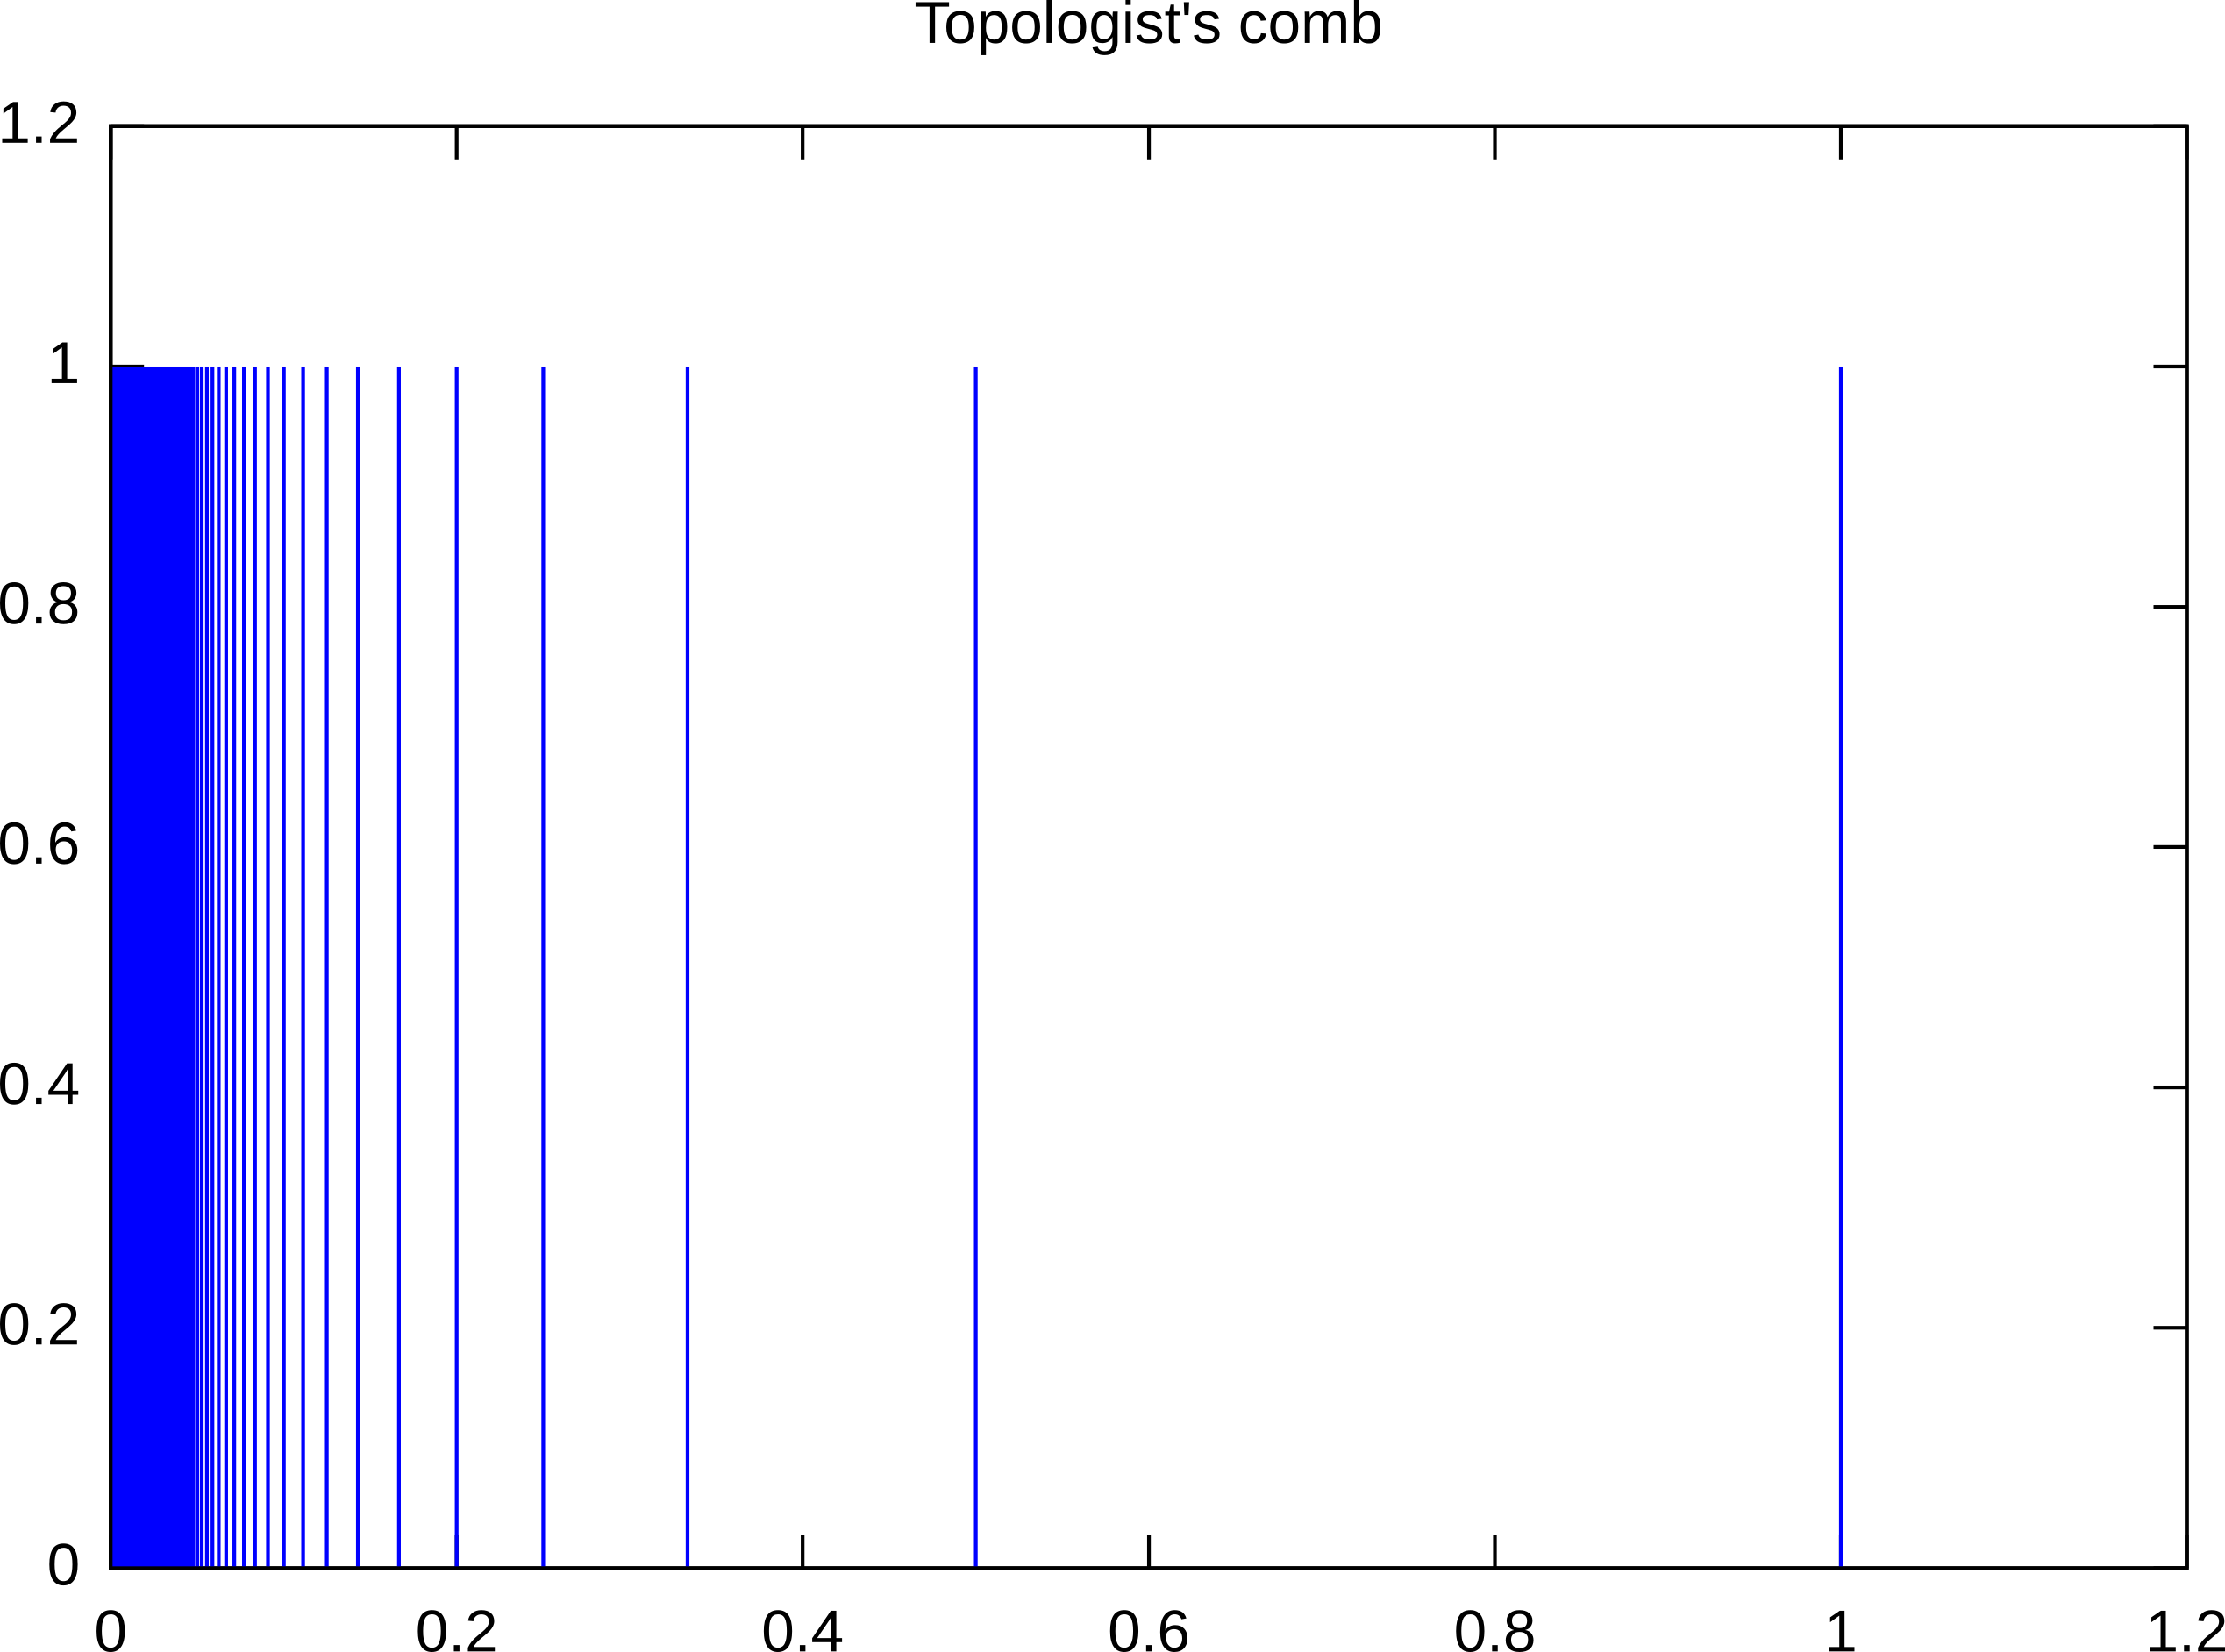
\includegraphics[width=0.5\linewidth]{images/topologia_generale/g160}
			\caption{Visualizzazione del pettine del topologo}
			\label{fig:comb_topology}
		\end{figure}
		
		
		Possiamo osservare che questo spazio è connesso. È ovvio che $D \setminus  \left\{(0,1)\right\}$ è connesso per archi e quindi è connesso, pertanto se fosse sconnesso le componenti sarebbero $(0,1)$ e $D \setminus \{(0,1)\}$. Ma $\overline{D \setminus \{(0,1)\}} \cap \{(0,1)\} \neq \varnothing$ e quindi tutto $D$ è connesso. \\ \\
		D'altro canto $D$ non è connesso per archi. Consideriamo $f$ funzione continua che connette $(0,1)$ a $(0,0)$, con $f(0) = (0,1)$. Mostriamo che $f^{-1}(D)$ è sconnesso, da cui per assurdo si arriva che $\left[0,1\right]$ è sconnesso. Allora vediamo che $f^{-1}(\left\{0\right\})$ è chiuso per definizione (un punto è chiuso e la controimmagine di un chiuso è chiuso se la mappa è continua). Per cui dobbiamo far vedere che $f^{-1}(\left\{(0,1)\right\})$ è aperto. Prendiamo un intorno di $(0,1)$ che chiameremo $U \subset D$ tale da non intersecare l'asse delle ascisse e lo supponiamo tale che $f^{-1}(U)$ è connesso. Allora 
		poiché $U$ non interseca l'asse delle ascisse, dev'essere che $x \in V$ tale da essere della forma $x = (1/n, k)$ per qualche $n \in \N$ e $k \in \left(0,1\right]$. Osserviamo che ogni intorno contiene almeno un elemento di questa forma (perché sappiamo che si `accumulano' su $(0,1)$). Per cui sia $x \neq (0,1)$ allora $x = (1/n, k) \in U$ per cui possiamo trovare $1/n+1< r< 1/n$ per cui possiamo vedere che la controimmagine di $U$ si può separare nei seguenti insiemi disgiunti 
		\begin{equation*}
			f^{-1}(U) = f^{-1}((-\infty, r)\times \left[0,1\right]) \cup f^{-1}((r,+\infty)\times \left[0,1\right])
		\end{equation*}
		Pertanto possiamo dire che $U$ è sconnesso contro la nostra ipotesi di connessione. Risulta quindi che $f^{-1}((0,1))$ è aperto e chiuso, ma $\left[0,1\right]$ è ovviamente connesso da cui dev'essere che $\{(0,1)\}$ non è connesso per archi a $\{(0,0)\}$.\\ 
		
		\begin{flushleft}
			\textbf{Seno del topologo}
		\end{flushleft}
		
		 Consideriamo la funzione reale 
		\begin{equation*}
			f(x) \coloneqq
			\begin{cases}
				0 & \text{se}\ x = 0 \\
				\sin \frac{1}{x} & \text{se}\ x \in \R^+
			\end{cases}
		\end{equation*}
		allora possiamo vedere in modo simile al pettine del topologo che l'immagine della funzione è connessa, ma il punto $(0,0)$ non è connesso per archi a nessun altro punto del grafo. Infatti se esistesse una funzione continua che collega le due parti del grafico avrebbe limite $\lim_{x\to 0} g(x) = \left[-1,1\right]$ e quindi non può essere continua in $0$.
\end{remark}

%todos: 4

\chapter{Esempi}



\section{Alcune varianti di topologie su $\R$}
\subsection{\textcolor{TopGener}{\textbf{Caratteristiche degli spazi compatti}}}



\begin{definition}
	D'ora in poi sia $\mathcal{B} = \left\{\left[a,b\right) \,\middle|\, a,b \in \R\right\}$ una base tale da generare la topologia $\tau_j$ sull'insieme $\R$.
\end{definition}

\begin{theorem}
	La topologia $\tau_j$ generata dalla base $\mathcal{B} \coloneqq \left\{ \left[a,b\right) \,\middle|\, a,b\in \R \right\}$ è strettamente più fine della topologia euclidea. 
\end{theorem}
\begin{proof}
	Ogni aperto di $\tau_{\text{euclidea}}$ è contenuto in $\tau_j$. Infatti sia $(a,b) \in \tau_{\text{euclidea}}$ allora prendo 
	\begin{equation*}
	(a,b) = \bigcup_{n \in \N} \left[a + \frac{1}{n}, b\right)
	\end{equation*}
	Ma l'aperto della $\left[0,1\right) \in \tau_j$ non appartiene a $\tau_{\text{euclidea}}$ poiché non è della forma $(a,b)$. \\ Segue che $\tau_j$ è strettamente più fine di $\tau_{\text{euclidea}}$.
\end{proof}

Allora valgono alcune proprietà già viste nei precedenti capitoli, tra cui il fatto di non avere basi numerabili, avere sistemi di intorni numerabili, essere più fine della topologia euclidea standard, ed altro come vedremo in questa sezione.

\begin{theorem}
	Le seguenti affermazioni sono vere in $\tau_j$.
	\begin{enumerate}
		\item L'intervallo $\left[0,1\right]$ è un chiuso in $\tau_j$. 
		\item La funzione $f \colon x \mapsto -x$ non è continua in $\tau_j$.
	\end{enumerate}
\end{theorem}
\begin{proof}\
	\begin{enumerate}
		\item Per dimostrare la chiusura bisogna far vedere che $\left[0,1\right]^c$ sia aperto. Ma questo è abbastanza facile. Infatti $\left[0,1\right]^c = \left(-\infty, 0\right) \cup \left(1, +\infty\right)$, per cui basta vedere che $\left(-\infty, 0\right) = \bigcup_{n \in \N} \left[-n, 1/(n+1)\right)$ e $\left(1, +\infty\right) = \bigcup_{n \in \N} \left[1+1/(n+1), n+2\right)$, per cui risulta che $\left[0,1\right]$ è un chiuso.
		\item La funzione è ovviamente non continua, infatti si consideri l'aperto $\left[0,1\right)$, la sua controimmagine attraverso $f$ è $\left(-1, 0\right]$ che non è aperto.
	\end{enumerate}
\end{proof}

\begin{theorem}
	L'insieme $\mathcal{B} = \left\{ \left[a, b\right] \,\middle|\, a \le b, a, b \in \R \right\}$ è una base su $\R$ e la topologia generata è quella discreta. 
\end{theorem}
\begin{proof}
	Dimostro che $\mathcal{B}$ è un ricoprimento di $\R$. Infatti basta prendere $\R = \bigcup^{+\infty}_{n=1} \left[-n, n\right]$. Inoltre se interseco due chiusi nella topologia euclidea è ancora un chiuso quindi ho la stessa cosa qui. Per cui $\mathcal{B}$ è una base. \\ 
	
	È ovvio che tutti i singoletti di $\R$ sono contenuti in $\mathcal{B}$ quindi $\mathcal{C}\subset \mathcal{B}$ dove $\mathcal{C}$ genera la topologia discreta e poiché è la più fine dev'essere che anche $\mathcal{B}$ generi la topologia discreta su $\R$.
\end{proof}



\subsection{\textcolor{TopGener}{\textbf{Un breve esercizio}}}



\begin{example}
	Definito l'insieme $$\mathcal{B} = \left\{A \in 2^\R \,\middle|\, 0 \notin A \right\} \cup \left\{ A \in 2^\R \,\middle|\, 0 \in A, \R \setminus A \; \text{finito} \right\}$$ calcolare la chiusura di $J = \left[1,2\right] \times \left\{0\right\}$. \\ \\
	È ovvio dimostrare che l'insieme oltre ad essere una base è anche una topologia. \\ Inoltre vale $\overline{J} = \overline{\left\{0\right\}} \times \overline{\left[1,2\right]}$, quindi posso separare i casi in una topologia $\mathcal{B}$. Vediamo che $\overline{\left\{0\right\}} = \left\{0\right\}$ per la definizione della topologia, $\left[1,2\right]$ è aperto e $\left[1,2\right] \cup \left\{0\right\}$ è chiuso (perché il complementare è aperto). \\ Segue che $\overline{\left[1,2\right]} = \left[1,2\right] \cup \left\{0\right\}$. Quindi ho trovato $\overline{J}$.
\end{example}
\begin{proof}
	
\end{proof}



\section{Topologia di Zariski e gli insiemi algebrici}
\subsection{\textcolor{TopGener}{\textbf{Una topologia aliena in un mondo noto}}}
%todo: inserire spiegazione di roba noetheriena



\begin{definition}
	Si definisce topologia di Zariski su $\R^n$ la topologia generata dall'insieme dei chiusi 
	\begin{equation*}
	\mathcal{F} \coloneqq \left\{ C \in 2^{\R^n} \,\middle|\, C \; \text{insieme algebrico} \right\}
	\end{equation*}
\end{definition}

\begin{theorem}
	Gli insiemi algebrici formano una famiglia di chiusi che generano una topologia per $\R$.
\end{theorem}
\begin{proof}\
	\begin{enumerate}
		\item I polinomi $f(x) = 0$ e $f(x) = 1$ danno come soluzioni rispettivamente gli insiemi $\R, \varnothing$.
		\item Bisogna dimostrare che l'intersezione di insiemi algebrici è ancora un insieme algebrico. Poiché tutti gli insiemi algebrici in $\R$ sono tutti finiti\footnote{Supponi che $X \neq \R$ sia algebrico e infinito allora esiste un polinomio che ha $\deg(f) \ge |X|$ ma i polinomi non possono avere grado infinito, assurdo.} tranne $\R$, l'intersezione di insiemi finiti sarà un insieme finito, per cui posso enumerare le soluzioni $\left\{x_1, \dots, x_n\right\}$ e quindi generare il polinomio $f(z) = (z-x_1)\cdots(z-x_n)$. Se l'intersezione è infinita è algebrico perché è $\R$. 
		\item L'unione agisce in modo più prevedibile. Infatti se $F_1, \dots, F_n$ sono algebrici allora esistono $f_1, \dots, f_n$ che li generano. Per cui $f = f_1 \cdots f_n$ è il polinomio che genera $F_1 \cup \dots \cup F_n$.
	\end{enumerate}
\end{proof}

\begin{theorem}
	Gli insiemi algebrici formano una topologia su $\R^n$.
\end{theorem}
\begin{proof}
	Analogamente alla dimostrazione in $\R$ si dimostra che
	\begin{enumerate}
		\item I polinomi $f(x_1, \dots, x_n) = 0$ e $f(x_1, \dots, x_n) = 1$ danno come soluzioni rispettivamente gli insiemi $\R^n, \varnothing$.
		\item Siano $F_1, \dots, F_n$ insiemi algebrici allora esistono $f_1, \dots, f_n$ che li generano. Per cui $f = f_1 \cdots f_n$ è il polinomio che genera $F_1 \cup \dots \cup F_n$.
		\item Questa parte è meno banale. Userò la notazione tratta dal libro W. Fulton, Algebraic Curves. Dimostro inannzitutto che se $\left\{I_i\right\}_{i \in \mathcal{I}}$ dove $I_i$ è un ideale di $\R\left[x_1, \dots, x_n\right]$\footnote{questo anello è \textbf{Noetheriano} poiché $\R$ è un campo.} per ogni $i$, allora 
		\begin{equation*}
			\bigoplus_{i \in \mathcal{I}} I_i = I
		\end{equation*}
		dove $I$ è un ideale di $\R\left[x_1, \dots, x_n\right]$. \\ Poiché siamo in un anello Noetheriano $I$, questo è un ideale per qualsiasi insieme indicizzante $\mathcal{I}$. 
		Per cui 
		\begin{equation*}
		\bigcap_{i \in I} A_i = \bigcap_{i \in I} V(I_i) = V\left(\bigoplus_{i \in \mathcal{I}} I_i\right) = V(I)
		\end{equation*}
		e poiché $I$ è un ideale ho anche che $V(I)$ è un insieme algebrico per definizione. \footnote{dal punto di vista della notazione $A_i = V(I_i)$ sta ad indicare che l'insieme algebrico $A_i$ è l'insieme delle soluzioni dell'ideale $I_i$, visto che ogni insieme algebrico è generato da almeno un ideale di polinomi}
	\end{enumerate}	
\end{proof}



\section{Esempio di quoziente}
\subsection{\textcolor{TopGener}{\textbf{Un breve esempio di quoziente topologico}}}
	


\begin{theorem}
	Si consideri $\left[0,1\right]$ con topologia euclidea indotta, dimostrare che $(\left[0,1\right]/R, \tau_{\text{euclidea}}|_{\left[0,1\right]/R}) \simeq (S^1, \tau_{\text{euclidea}}|_{S^1})$ dove $R$ è la relazione che associa $xRy \Leftrightarrow x = y \lor |x - y| = 1$
\end{theorem}
\begin{proof}
	Possiamo usare uno dei corollari (come il \textit{primo teorema di omeomorfismo}) costruiti negli spazi quozienti. Per cui ci basta trovare un identificazione $\morphism{f}{\left[0,1\right]}{\S^1}$ e la scelta più naturale ricade su 
	\begin{equation*}
		f(x) = (\cos 2\pi x, \sin 2 \pi x)
	\end{equation*}
	che è suriettiva, continua sulla topologia euclidea e vale $f^{-1}f(x) = \left[x\right]_R$. Meno banale è dimostrare che $\tau_f = \tau_{\text{euclidea}}|_{S^1}$. Usando il teorema \ref{thr:freeomeombyquo}
\end{proof}



\section{Discriminazione di topologie}
\subsection{\textcolor{TopGener}{\textbf{Discriminare, ma in senso buono}}}



Non è sempre facile dimostrare che due topologie sono la stessa a meno di omeomorfismi. \\ Per questo se si hanno degli strumenti per riuscire a discriminare quelle distinte \textit{al volo}, si può ridurre il tempo perso a dimostrare che due topologie distinte siano la medesima. \\ \\A tal fine nei capitoli precedenti si sono sviluppate alcune proprietà che sono invarianti per omeomorfismi e dunque degli invarianti topologici. Vediamo una semplice carrellata di come possono essere utilizzati per discriminare le topologie distinte

\begin{theorem}
	Le seguenti affermazioni sono vere:
	\begin{enumerate}
		\item $\left[0,1\right] \not\simeq (0,1)$
		\item $\left[0,1\right] \not\simeq \R$
		\item $\left(0,1\right] \not\simeq (0,1)$
		\item $\left[0,1\right]^2 \not\simeq \left[0,1\right]$
		% TODO $\R \simeq (0,1)$??? dal punto di vista della connessione e della compattezza sembrerebbe funzionare
	\end{enumerate}
\end{theorem}
\begin{proof}\
	\begin{enumerate}
		\item La compattezza è un'invariante per omeomorfismi, quindi se le due topologie fossero la medesima avrei che $(0,1)$ compatto se e solo se $\left[0,1\right]$ lo è. Ma $\left[0,1\right]$ è compatto, mentre $(0,1)$ non lo è. Pertanto non possono essere omeomorfi.
		\item Usando ancora una volta la compattezza come invariante topologico si vede che $\R$ non è compatto mentre $\left[0,1\right]$ lo è, pertanto non possono essere omeomorfi.
		\item La connessione è un altro invariante topologico. Infatti supponiamo che $\left(0,1\right]$ sia omeomorfo a $\left(0,1\right)$. Allora esiste $f(\left(0,1\right]) = \left(0,1\right)$ e $f(1) = x \in (0,1)$. Quindi se si considera $\morphism{f}{(0,1)}{(0,1)\setminus \left\{x\right\}}$ di sicuro $x$ è interno a $(0,1)$, quindi dev'essere che $(0,1) \setminus \left\{x\right\} = (0, x) \cup (x, 1)$. Bisogna far notare che $f$ è ancora un omeomorfismo tra $(0,1)$ e $(0,1)\setminus \left\{x\right\}$ (è ovviamente bigettiva e manda aperti in aperti anche se manca un punto). Eppure $(0,1)$ è connesso e quindi $f((0,1))$ dovrebbe essere connesso, ma non lo è. \\ Pertanto non può esistere $f$ omeomorfismo.
		\item Analogo al caso precedente. Infatti si prenda un punto interno di $x \in (0,1)$, indipendentemente da dove verrà mappato su $\left[0,1\right]^2$, $\left[0,1\right]^2 \setminus \left\{f(x)\right\}$ sarà ancora connesso\footnote{È ovvio che sarà ancora connesso: se $x$ viene mappato sul bordo, allora essendo $(0,1)^2$ connesso e $\left[0,1\right]^2$ connesso segue che qualsiasi $Z$, tale che $(0,1)^2 \subset Z \subset \left[0,1\right]^2$ è ancora connesso; se $x$ è interno invece posso sempre trovare una funzione continua che aggira $x$ e collega ogni paio di punti di $\left[0,1\right]^2 \setminus \left\{f(x)\right\}$}, mentre $\left[0,1\right] \setminus \left\{x\right\}$ non lo è. 
	\end{enumerate}
\end{proof}

%todos: 1



\part{Topologia Algebrica}
\chapter{Omotopie: mappe tra cammini}
Concluso lo studio della topologia generale, vogliamo applicarla in un campo molto importante della matematica: la \textit{topologia algebrica}. \\ \\ Studieremo la struttura degli spazi (in particolare le superfici topologiche compatte): perché una tazza è un toro? per quale ragione una palla non è un toro? e soprattutto, a chi è venuto in mente di chiamare \enquote{toro} una ciambella?\\ Conosciamo la risposta all'ultima - gli antichi romani, deriva dal nome di un cuscino a forma di ciambella - ma per tutte le altre e molte di più addentriamoci nel mondo della topologia algebrica! \\ \\ In seguito riusciremo anche ad applicare le nuove strutture matematiche nella classificazione delle varietà.



\newpage
\section{Omotopie e retratti}
Cosa pensereste se qualcuno vi dicesse che può schiacciare una lattina rendendola un disco? Giochi da bambini, vero? \\ Beh, ora faremo la stessa cosa \dots ma con la matematica.
\subsection{\textcolor{TopAlg}{\textbf{Omotopie e classi di omotopia}}}
Vogliamo definire formalmente il concetto di \enquote{trasformare con continuità} due funzioni tra loro.

\begin{definition}
	Siano $\morphism{f_0, f_1}{X}{Y}$ mappe continue. Allora $f_0$ e $f_1$ si dicono \textbf{omotope} se esiste una funzione continua $\morphism{F}{X \times \left[0,1\right]}{Y}$ tale che $F(t,0) = f_0(t)$ per ogni $t \in X$ e $F(t,1) = f_1(t)$ per ogni $t \in X$.
\end{definition}

\begin{remark}[Omotopia come relazione di equivalenza]
	L'omotopia è una relazione di equivalenza.\\ Le prime due proprietà sono immediate, per la proprietà transitiva basta comporre le omotopie.
\end{remark}

\begin{definition}
	Siano $\morphism{f_0, f_1}{X}{Y}$ mappe continue e sia $A \subset X$. Allora $f_0$ e $f_1$ si dicono \textbf{omotope relativamente ad} $A$ se esiste una funzione continua $\morphism{F}{X \times \left[0,1\right]}{Y}$ tale che $F(t,0) = f_0(t)$ per ogni $t \in X$ e $F(t,1) = f_1(t)$ per ogni $t \in X$ e $F(a, t) = f_0(a) = f_1(a)$ per ogni $a \in A$.
\end{definition}

\begin{definition}
	Due spazi topologici $X,Y$ si dicono \textbf{omotopicamente equivalenti} se esistono le mappe continue $\morphism{f}{X}{Y}$, $\morphism{g}{Y}{X}$ tali che $g \circ f \sim \operatorname{Id}_X$ e $f \circ g \sim \operatorname{Id}_{Y}$. \\ In particolare si dice che \textit{sono nella stessa classe di omotopia} (o \textit{hanno la stessa classe di omotopia})
\end{definition}

\begin{remark}[Equivalenza omotopica]
	L'omotopia di spazi topologici è una relazione di equivalenza, si dimostra come in precedenza; non è difficile.
\end{remark}

\begin{remark}[Possibili fraintendimenti] Nonostante spesso e volentieri sia comodo pensare alla \enquote{deformazione continua} come una deformazione fisica dello spazio, è immediato verificare come \textbf{effettivamente non lo sia}. Notiamo che riferendoci agli spazi con \textit{deformazione continua} reciproca si intende il passaggio tra rappresentanti diversi della stessa classe di omotopia. \\ Si prenda una circonferenza con un punto esterno (spazio $A$) ed una circonferenza con un punto interno (spazio $B$), ovviamente sono nella stessa classe di omotopia. Però è impossibile deformarli \enquote{manualmente} fino ad ottenerli a vicenda, perché qualunque deformazione si compia prima o poi il punto interseca la circonferenza: in questo modo otterremmo uno spazio diverso sia da $A$ che da $B$, che non si trova neanche nella stessa classe di omotopia.
\end{remark}

\newpage
\subsection{\textcolor{TopAlg}{\textbf{Retratti e retratti di deformazione}}}

\begin{definition}
	Se $A \subset X$ dove $X$ spazio topologico allora $A$ è detto \textbf{retratto} di $X$ se esiste $\morphism{r}{X}{A}$ con $r$ continua e che $r(a) = a$ per ogni $a \in A$. In particolare $r \circ i_A = \operatorname{Id}_{A}$. \\ 
	In particolare	$A$ è detto \textbf{retratto di deformazione} di $X$ se è un retratto e $i_A \circ r \sim \operatorname{Id}_{X}$.\\ Ovviamente se è retratto di deformazione vuol dire che si trovano nella stessa classe di omotopia.
\end{definition}


\begin{remark}
	Alcuni esempi
	\begin{enumerate}
		\item Dimostriamo che $\R^n \setminus \{0\} \sim \S^{n-1}$. \\ Definiamo come retratto $\morphism{r}{\R^n \setminus \{0\}}{\S^{n-1}}$ con $r(x) = \frac{x}{\|x\|}$. Allora è ovvio che $r \circ i = \operatorname{Id}_{\S^{n-1}}$. Prendiamo quindi il caso $i \circ r = \frac{x}{\|x\|}$ con $x \in \R^n  \setminus \{0\}$. Dimostriamo che questa funzione è omotopa all'identità su $\R^n \setminus \{0\}$. Usiamo l'omotopia 
		\begin{equation*}
		F(s,t) = (1-t)(i \circ r) + tx
		\end{equation*} 
		ed abbiamo concluso.
		\item Definiamo ora la somma topologica di due spazi topologici $(X, \tau_1)$, $(Y, \tau_2)$ disgiunti. L'unione verrà definita come $(X \cup Y, \tau)$ dove $\tau$ è la topologia i cui aperti sono tali per cui $A \in \tau$ allora $A \cap X \in \tau_1$ e $A \cap Y \in \tau_2$. La somma topologica vera e propria $X \lor Y$ è definita come 
		\begin{equation*}
		X \lor Y := (X \cup Y, \tau) / \sim_{a_0, b_0}
		\end{equation*}
		dove $ a \sim_{a_0, b_0} b \iff a = b \lor (a = a_0 \land b = b_0)$. Ovvero unisce gli spazi e fa coincidere un punto dei rispettivi nello stesso. In pratica consideriamo il bouquet di due circonferenze $\S^1 \lor \S^1$ rappresentato in figura.
		
		\begin{figure}[h]
			\centering
			
\includegraphics[width=0.3\linewidth]{images/topologia_algebrica/bouquet_circonferenze}
			\caption{}
			\label{fig:bouquetcirconferenze}
		\end{figure}
		Questo è ovviamente omotopo a $\R^2 \setminus \{(-1,0), (1,0)\}$ dove i punti scelti possono essere presi a piacere.
		\item Se $X \subset \R^n$ ed è un sottospazio stellato rispetto al centro $x_0$ allora $Y = \{x_0\}$ è un retratto di $X$. Infatti $X \sim \{p\}$ per qualsiasi $p \in \R^n$. Mostriamo intanto che $Y \sim X$. L'omotopia $F(x,t) = x - t(x-x_0)$ porta, in modo continuo, dalla funzione di $\morphism{id}{X}{X}$ (ovvero $x \mapsto x$) a $\morphism{i}{X}{X}$ (ovvero $x \mapsto x_0$). Ovvero $Y \sim X$.
		\item Sia $X = T$ toro. Allora $\morphism{r}{T}{\S^1}$ è un retratto su $\S^1 \subset T$, ma non è un retratto di deformazione. Infatti è impossibile trasformare (in modo continuo) un toro in una circonferenza. 
		\item Se si toglie un punto a il $g$-toro allora $T_g \setminus \{t\} \sim \underbrace{\S^1 \wedge \dots \wedge \S^1}_{2g-\text{volte}}$ 
		\item Analogamente per il piano proiettivo $U_h$, una volta tolto un suo punto ed ottenuto $U_h \setminus \{p\} \sim \underbrace{\S^1 \wedge \dots \wedge \S^1}_{h-\text{volte}}$
 	\end{enumerate}
\end{remark}

\newpage
\section{CW-complessi}
\subsection{\textcolor{TopAlg}{\textbf{Una semplice classe di spazi complessi}}}

Ora verranno introdotte delle classi di insiemi tali che possono essere suddivisi in parti \textit{retratte} e parti irriducibilmente non retratte, si veda il Teorema \ref{thr:contrai_ncelle_cw_complesso}.

\begin{definition}
	Uno spazio topologico $X$ si dice n-\textbf{cella} se $X \simeq \D^n$.
\end{definition}

\begin{definition}[Procedura di incollamento]
	\label{def:incollamento}
	L'incollamento di due spazi topologici $X,Y$ tramite $A \subset X$ è rapprensentato dal seguente diagramma
	\begin{equation*}
	\begin{tikzcd}
	A \arrow[d, hook]{i} \arrow[r]{f} & Y \\
	X
	\end{tikzcd}
	\end{equation*} 
	\begin{itemize}
		\item $f: A \to Y$ funzione \enquote{di incollamento}
		\item $i: A \to X$ inclusione
	\end{itemize}
	Lo spazio topologico risultante dall'incollamento è $X \sqcup Y / \sim$ dove usiamo la relazione $x \sim y \in Y \Longleftrightarrow x \in A \land f(x) = y$.
\end{definition}

\begin{remark}[Algoritmo di costruzione di un CW-complesso finito]
	$X$ è un CW-complesso se è possibile costruirlo secondo il seguente algoritmo:
	\begin{enumerate}
		\item Sia dato $X^0 \neq \varnothing$ insieme finito (detto anche $0$-scheletro)
		\item Sia $n \ge 1$, allora per ipotesi induttiva supponiamo di avere un $X^{n-1}$, ovvero un $(n-1)$-scheletro. Allora si incollano a $X^{n-1}$ delle $n$-celle attraverso il procedimento della Definizione \ref{def:incollamento} in cui vale 
		\begin{equation*}
		\begin{tikzcd}
			\S^{n-1} = \partial \D^n \arrow[d, hook]{i} \arrow[r]{f} & X^{n-1} \\
			\D^n
		\end{tikzcd}
		\end{equation*} 
		con $X^n = X^{n-1} \sqcup \D^n / \sim$ con la relazione specificata nella procedura di incollamento.
		\item Se il CW-complesso è di dimensione $N$, allora per $n = N$ il procedimento termina, con $X^N = X$.  
	\end{enumerate}
\end{remark}

\begin{definition}
	Sia $X$ un CW-complesso allora una \textbf{n-cella chiusa} in $X$ è l'immagine di $\morphism{f}{\D^n}{X}$ dove $f$ è definita come nella seguente successione
	\begin{equation*}
	\begin{tikzcd}
		\D^n \arrow[bend right=25, swap, hook]{rr}{f} \arrow[r,hook] & \D^n \sqcup X^{n-1} / \sim \arrow[r,hook] & X
	\end{tikzcd}
	\end{equation*}
\end{definition}

\begin{remark}
	In generale $\image{f} \neq \D^n$. Per esempio si prenda la costruzione di $\S^2$ come un CW-complesso con una $0$-cella e una $2$-cella che identifica tutto il suo bordo nel punto. Allora 
	\begin{equation*}
	\begin{tikzcd}
		\D^2 \arrow[bend right=25, swap, hook]{rr}{f} \arrow[r,hook] & \D^2 \sqcup \{p\} / \sim \arrow[r,hook] & \S^2
	\end{tikzcd}
	\end{equation*}
	è ovvio che $\image{f} = \S^2 \neq \D^2$. 
\end{remark}

\begin{definition}
	Sia $X$ un CW-complesso allora una n-cella aperta in $X$ è l'immagine di $\morphism{f}{\D^n}{X}$ dove $f$ è definita come nella seguente successione
	\begin{equation}
	\begin{tikzcd}
	\mathring{\D}^n \arrow[bend right=25, swap, hook]{rr}{f} \arrow[r,hook] & \mathring{\D}^n \sqcup X^{n-1} / \sim \arrow[r,hook] & X
	\end{tikzcd}
	\end{equation}
\end{definition}

\begin{remark}
	Le $n$-celle aperte sono omeomorfe al disco aperto $\mathring{\D}^n$. Infatti 
	\begin{equation*}
		\mathring{\D}^n \sqcup X^{n-1} / \sim\ = \mathring{\D}^n \sqcup X^{n-1}
	\end{equation*}
	poiché il bordo non dev'essere identificato (non fa parte dell'insieme $\mathring{\D}^n$).
\end{remark}

\begin{theorem}
	\label{thr:contrai_ncelle_cw_complesso}
	Se $X$ è un CW-complesso e $A \subset X$ è un sottocomplesso chiuso (ovvero un unione di $n$-celle chiuse) vale che se $A$ è contraibile allora $X$ è omotopo a $X / A$.
\end{theorem}
\begin{proof}
	Si può costruire la relazione di equivalenza utilizzando un po' di teoria dei grafi: sia data la foresta $F$ del grafo, intuitivamente si tratta del risultato della costruzione del CW-complesso una volta \enquote{elencati} i passaggi svolti su un diagramma ad albero. \\ Allora posso quozientare $X$ con la relazione di equivalenza
	\begin{equation*}
	x \sim y \iff \text{ hanno un albero in comune in $F$ }
	\end{equation*}
	La mappa quoziente $X \to X/\sim$ è una equivalenza omotopica. \\ Si noti inoltre che lo spazio quoziente eredita la struttura di CW-complesso. \\ \\ Ovviamente questa è solo un'idea di dimostrazione, la vera dimostrazione può essere svolta usando molta più teoria di algebra e sfruttando l'ipotesi di contraibilità (il modo in cui si usa è ovvio).
\end{proof}

I CW-complessi sono importanti poiché è possibile esprimere un invariante topologico. Infatti se due CW-complessi sono omeomorfi allora il valore della funzione caratteristica di Eulero è uguale. \\ Notiamo che usiamo i CW-complessi finiti perché sono compatti, e noi vogliamo classificare gli spazi compatti.

\begin{definition}
	Sia $X$ un CW-complesso costituito da $n_0$ $0$-celle, $\dots$, $n_N$ $N$-celle, allora 
	\begin{equation*}
		\chi(X) = \sum_{i=0}^{N} (-1)^i n_i
	\end{equation*}
	è la \textbf{funzione caratteristica di Eulero} di $X$. 
\end{definition}

\begin{remark}
	Alcuni esempi di CW-complessi
	\begin{enumerate}
		\item In generale un $g$-toro è composto da $1$ $0$-cella, $2g$ $1$-celle, $1$ $2$-cella. Quindi ha numero caratteristico $\chi(T_g) = 2(1-g)$. 
		\item In generale un piano proiettivo $U_h$ è composto da $1$ $0$-cella, $h$ $1$-celle, $1$ $2$-cella. Quindi ha numero caratteristico $\chi(U_h) = 2 - h$.
		\item Il disco $\D^n$ è una $n$-cella quindi $\chi(\D^n) = (-1)^n$. In generale il disco $n$-esimo si può costruire con una $0$-cella, una $(n-1)$-cella e $1$ $n$-cella.
	\end{enumerate}
\end{remark}

\begin{remark}
	Alcuni esempi del Teorema \ref{thr:contrai_ncelle_cw_complesso} possono essere i seguenti
	\begin{enumerate}
		\item Sia $X \subset \R^2$ come in figura 
		\begin{figure}[H]
			\centering
			
\includegraphics[width=0.6\linewidth]{images/topologia_algebrica/CWCOMPLEXEsempio1}
			\caption{}
			\label{fig:cwcomplexesempio1}
		\end{figure}
		allora è omotopicamente equivalente a un buquet di due circonferenze se si identifica la $1$-cella del diametro in un punto da cui
		\begin{figure}[H]
			\centering
			
\includegraphics[width=0.6\linewidth]{images/topologia_algebrica/CWCOMPLEXEsempio2}
			\caption{}
			\label{fig:cwcomplexesempio2}
		\end{figure}
		\item Sia $X \subset \R^2$ come in figura 
			\begin{figure}[H]
				\centering
				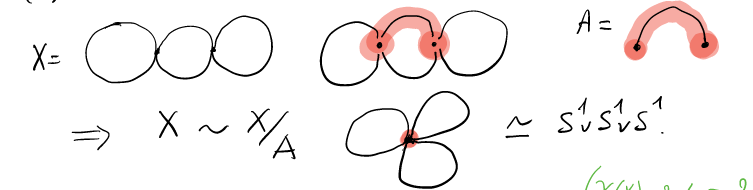
\includegraphics[width=0.7\linewidth]{images/topologia_algebrica/CWCOMPLEXEsempio3.png}
				\caption{}
				\label{fig:cwcomplexesempio3}
			\end{figure}
			identifichiamo una 1-cella della circonferenza centrale (l'insieme $A$) in un punto così da ottenere un bouquet di $3$ circonferenze per il Teorema \ref{thr:contrai_ncelle_cw_complesso}.   
		\item Sempre contraendo come in figura è abbastanza esplicito  che il grafo sia omotopo a un buquet di $4$ circonferenze.
			\begin{figure}[H]
				\centering
				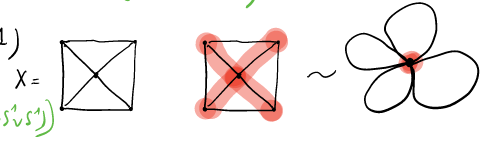
\includegraphics[width=0.7\linewidth]{images/topologia_algebrica/CWCOMPLEXEsempio8.png}
				\caption{}
				\label{fig:cwcomplexesempi4}
			\end{figure}
		\item Sia $X$ un toro con un disco e una circonferenza 
			\begin{figure}[H]
				\centering
				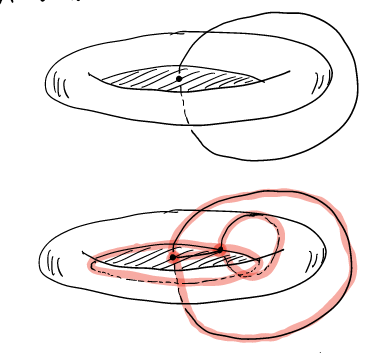
\includegraphics[width=0.3\linewidth]{images/topologia_algebrica/CWCOMPLEXEsempi4}
				\caption{}
				\label{fig:cwcomplexesempi4}
			\end{figure}
			Allora $X$ è un CW-complesso composto da $2$ $0$-celle, $4$ $1$-celle, $2$ $2$-celle. Posso contrarre il disco al centro del toro in un punto (perché possiamo è un retratto).   
			\begin{figure}[H]
				\centering
				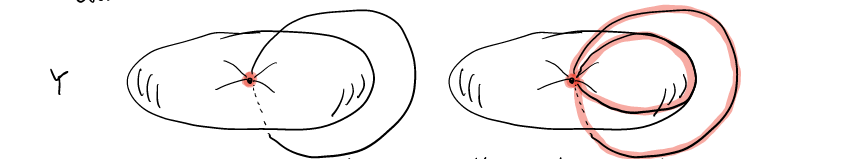
\includegraphics[width=0.7\linewidth]{images/topologia_algebrica/CWCOMPLEXEsempi5}
				\caption{}
				\label{fig:cwcomplexesempi4}
			\end{figure}
			Indichiamo con $Y$ l'insieme con il disco retratto in un punto. Poi \textit{allarghiamo} il toro in modo tale da ottenere una sfera con dentro parte della circonferenza identificata, otteniamo uno spazio omotopo allo spazio $Z$ come in figura
			\begin{figure}[H]
				\centering
				
\includegraphics[width=0.7\linewidth]{images/topologia_algebrica/CWCOMPLEXEsempi6}
				\caption{}
				\label{fig:cwcomplexesempi4}
			\end{figure}
			e studiando $Z$ si ottiene uno spazio omotopicamente equivalente a $\S^2 \lor \S^1 \lor \S^1$
			\begin{figure}[H]
				\centering
				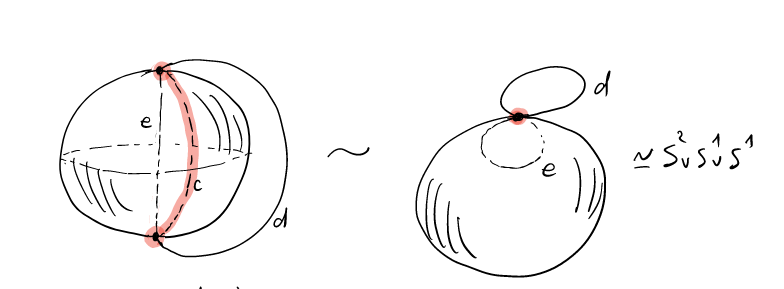
\includegraphics[width=0.7\linewidth]{images/topologia_algebrica/CWCOMPLEXEsempi7}
				\caption{}
				\label{fig:cwcomplexesempi4}
			\end{figure}
	\end{enumerate}
\end{remark}

\newpage
\section{Il gruppo fondamentale}
Esiste un gruppo che possiamo \enquote{incollare} ad uno spazio e che ne raccoglie le proprietà. In che senso \textit{ne raccoglie le proprietà}? \\ E soprattutto, come si costruisce? \\ Avendo struttura di gruppo è bene vedere alcuni teoremi puramente algebrici prima di continuare.
\subsection{\textcolor{TopAlg}{\textbf{Deformare cappi su una superficie}}}

\begin{definition}
	Sia $X$ spazio topologico, allora $\morphism{\alpha}{\left[0,1\right]}{X}$ tale che $\alpha(0) = x_0 \in X$ e $\alpha(1) = x_0 \in X$ con $\alpha$ continua si dice \textbf{cappio} di punto base $x_0$.
\end{definition}

\begin{definition}[Gruppo fondamentale] Sia $X$ uno spazio topologico, $x_0$ un punto appartenente ad $X$. Diciamo \textbf{gruppo fondamentale} di $X$ rispetto ad $x_0$ l'insieme delle classi di equivalenza omotopica dei cappi contenuti in $X$ con punto base $x_0$.
	\begin{equation*}
	\pi_1(X,x_0)= \left\{[\alpha] \ \big| \ \alpha \text{ è un cappio in $X$ di base $x_0$}\right\}
	\end{equation*}
	\begin{itemize}
		\item Uno spazio topologico $X$ si dice \textbf{semplicemente connesso} se $\pi_1(X, x_0) \simeq (\{1\}, +)$ ovvero il gruppo banale. 
	\end{itemize}
\end{definition}

\begin{definition}[Concatenazione di cammini]
	Definiamo l'operatore $*$ come la composizione delle classi omotopiche di cappi $\alpha, \beta$ (aventi estremi congiungibili) come segue
	\begin{equation*}
	\alpha * \beta :=
	\begin{cases}
		\alpha(2s) \quad 0 \le s \le 1/2 \\
		\beta(2s - 1) \quad 1/2 < s \le 1 \\ 
	\end{cases}
	\end{equation*}
\end{definition}

\begin{theorem}
	Siano $\alpha, \beta$ due cammini in $X$ tali che sia definito il prodotto e analogamente per i cammini $\gamma, \delta$. Allora se $\alpha \sim \gamma$ e $\beta \sim \delta$ vale $\alpha * \beta \sim \gamma * \delta$
\end{theorem}
\begin{proof} Basta scrivere l'omotopia: sia $F$ la prima e $G$ la seconda, l'omotopia cercata è
	\begin{equation*}
	H(s,t)=\begin{cases}
	F(2s,t) \ \ & 0 \leq s \leq \frac{1}{2}\\
	G(2s-1,t) \ \ & \frac{1}{2} \leq s \leq 1
	\end{cases}
	\end{equation*}
\end{proof}

\begin{theorem}
	$\pi_1(X, x_0)$ ha struttura di gruppo rispetto alla concatenazione di cammini. 
	\begin{equation*}
	(\pi_1(X, x_0), *) \ \text{è un gruppo}
	\end{equation*}
	In particolare, indicando con $x_k$ il cammino costante nel punto $x_k$ con un lieve abuso di notazione (altra notazione classica è $\varepsilon_{x_k}$), valgono
	\begin{enumerate}
		\item $x_0 * \alpha \sim \alpha \sim \alpha * x_1$
		\item $\alpha * \overline{\alpha} \sim x_0 \sim \overline{\alpha} * \alpha$.
		\item $(\alpha * \beta) * \gamma \sim \alpha * (\beta * \gamma)$
	\end{enumerate} 
\end{theorem}
\begin{proof} Verifichiamo intanto che riparametrizzando un cammino $\alpha$ non ne cambio la classe. Sia $\varphi:I \to I$ parametrizzazione continua, $\varphi(0)=0$ e $\varphi(1)=1$. La classe di omotopia non varia perché posso sempre scrivere l'omotopia
	\begin{equation*}
	F(s,t)=\alpha\big((1-t)s+t\varphi(s) \big)
	\end{equation*} 
	Allora posso dimostrare il teorema.
	\begin{enumerate}
		\item Basta trovare delle parametrizzazioni, la prima è
		\begin{equation*}
		\varphi(s)=
		\begin{cases}
		0 &  0 \leq s \leq \frac{1}{2}\\
		2s-1 &  \frac{1}{2} \leq s \leq 1\\
		\end{cases}
		\end{equation*}
		e la seconda 
		\begin{equation*}
		\varphi(s)=
		\begin{cases}
		2s  &  1 \leq s \leq \frac{1}{2}\\
		2s-1 &  \frac{1}{2} \leq s \leq 1\\
		\end{cases}
		\end{equation*}
		\item Trovare l'omotopia è banale, basta usare $\varepsilon_{x_0}$.
		\item Basta riparametrizzare in modo che
		\begin{equation*}
		(\alpha * \beta) * \gamma = \left((\alpha * \beta) * \gamma\right)\circ \varphi \sim \alpha * (\beta * \gamma)
		\end{equation*}
	\end{enumerate}
\end{proof}

\begin{theorem}
	Sia $X$ spazio topologico tale che $x_0 \in X$ è connesso per archi ad $x_1 \in X$, allora $\pi_1(X, x_0) \simeq \pi_1(X, x_1)$
\end{theorem}
\begin{proof} Sia $f$ l'arco congiungente i due punti, usiamo $u_f$ funzione tra i due gruppi fondamentali tale che
	\begin{equation*}
	u_f\left([\alpha]\right)=[(\overline{f}*\alpha)*f]
	\end{equation*}
	\begin{itemize}
		\item \textbf{Ben definita}\\
		Se $a \sim b$ allora $f*a \sim f*b$ e $(\overline{f}*a)*f=(\overline{f}*b)*f $ per quanto appena dimostrato.
		\item \textbf{Omomorfismo di gruppi}
		\begin{align*}
		u_f\left([a][b]\right)& =u_f\left([a*b]\right)=\left[\left(\overline{f}*(a*b)\right)*f\right]
		\end{align*}
		\begin{align*}
		u_f([a])\cdot u_f([b]) & = \dots \\
		& = \left[\left((\overline{f}*a)*f\right)*\left((\overline{f}*b)*f\right)\right]\\
		& = \left[\left(\overline{f}*\left((a*f)*(\overline{f}*b)\right)\right)*f\right]\\
		& = \left[\left(\overline{f}*(a*b)\right)*f\right]
		\end{align*}
		\item \textbf{Isomorfismo di gruppi}\\
		Ovvio, basta usare $u_{\overline{f}}$.
	\end{itemize}
\end{proof}

\begin{corollary}
	Se $X$ è connesso per archi allora il suo gruppo fondamentale è unico al più per isomorfismi.
\end{corollary}

\begin{proof} Particolarmente ovvio, inclusa solo per completezza; se lo spazio è connesso per archi vuol dire che la componente connessa per archi più grande è lo spazio stesso e per teorema esiste un arco tra ogni punto scelto a piacere verso ogni altro punto.
\end{proof}	
	
\begin{theorem}
	Sia $\morphism{\varphi}{X}{Y}$ una mappa continua tra spazi topologici, allora induce un omomorfismo tra i relativi gruppi fondamentali 
	\begin{align*}
	\varphi_*:\pi_1(X, x_0)&\to\pi_1(Y, \varphi(x_0))\\
	[\alpha] &\to [\varphi \circ \alpha]
	\end{align*}
	Inoltre l'operatore $_*$ gode delle \textit{proprietà funtoriali}:
	\begin{enumerate}
		\item $(\varphi \circ \psi)_* = \varphi_* \circ \psi_*$
		\item $(\operatorname{Id}_{X})_* = \operatorname{Id}_{\pi_1(X, x_0)}$ 
	\end{enumerate}
\end{theorem}
\begin{proof} Osserviamo che il morfismo indotto è ben definito.  
	\begin{equation*}
	a \sim b \implies \varphi\circ a \sim \varphi\circ b
	\end{equation*}
	infatti data $F$ prima omotopia basta usare $G=\varphi\circ F$. Risulta immediato anche dimostrare che è effettivamente un morfismo di gruppi, basta notare che $\varphi\circ(a*b)=(\varphi\circ a)*(\varphi\circ b)$.
\end{proof}

\begin{corollary}
	Se $\morphism{\varphi}{X}{Y}$ è un omeomorfismo di spazi topologici allora $\varphi_*$ è un isomorfismo di gruppi. In particolare il gruppo fondamentale è un \textit{invariante topologico}.
\end{corollary}

\begin{proof}
	Sia $f$ funzione continua che induce il morfismo $f_*$. \\ Allora per $x\in X$:
	\begin{align*}
	\left(f^{-1}\right)_*\circ f_* = \left(f^{-1}\circ f_*\right)=\operatorname{Id}_{\pi({X,x})}
	\end{align*}
	\begin{align*}
	f_*\circ\left(f^{-1}\right)_*  = \left(f_*\circ f^{-1} \right)=\operatorname{Id}_{\pi({Y,f(x)})}
	\end{align*}
\end{proof}

\begin{theorem}
	Se $A \subset X$ è un retratto di $X$ con $r$ come retrazione, allora vale che $\pi_1(A, x_0) \subset \pi_1(X, x_0)$ ed è un sottogruppo.  \\ In particolare $r_*\circ i_* =\operatorname{Id}_{\pi_{A,a}}$.
\end{theorem}
	\begin{proof}Particolarmente ovvio, basta scrivere:
		\begin{equation*}
		r_*\circ i_* =(r\circ i)_* = (\operatorname{Id}_{A})_*=\operatorname{Id}_{\pi({A,a})}
		\end{equation*}
		Per ogni retratto $A$ inoltre $i_*$ è un isomorfismo del suo gruppo fondamentale con immagine un sottogruppo di $\pi(X,a)$.
	\end{proof}

\subsection{\textcolor{TopAlg}{\textbf{Il teorema di invarianza omotopica}}}
Vogliamo dimostrare un risultato potente: il gruppo fondamentale è invariante omotopico. Per farlo dobbiamo sviluppare ulteriormente la teoria.
\begin{lemma}
	Siano $\Phi$ e $\Psi$ funzioni continue ed omotope tra $X$ ed $Y$, $F$ loro omotopia. Sia $f(t)=F(x_0,t)$ cammino tra $\Phi(x_0)$ e $\Psi(x_0)$ per il punto $x_0\in X$. Allora il seguente diagramma commuta (questo vuol dire che $\Psi_*=u_f\circ \Phi_*$).
	\begin{equation*}
	% https://tikzcd.yichuanshen.de/#N4Igdg9gJgpgziAXAbVABwnAlgFyxMJZABgBpiBdUkANwEMAbAVxiRAB120sAKADVIAPAPrEAlCAC+pdJlz5CKAEzkqtRizaduPAJqlOABQAWvEeInTZ2PASIBGUvbX1mrRBy699R7D3NilmowUADm8ESgAGYAThAAtkhkIDgQSCogDHQARjAMhnK2iiBYYNiwINSumh6+WMIAVFIyILEJSdSpSI6ZOXkFNgpspeWsVRrunib1TVatcYmIPV2IGVm5+YVDHiNYFeNubEzCUVIUkkA
	\begin{tikzcd}
	{\pi(X,x_0)} \arrow[rd, "\Psi_*" description] \arrow[rr, "\Phi_*" description] &                    & {\pi(Y,\Phi(x_0))} \arrow[ld, "u_f" description] \\
	& {\pi(Y,\Psi(x_0))} &                                                 
	\end{tikzcd}
	\end{equation*}
\end{lemma}
\begin{proof} Devo mostrare che per ogni $A=[a]\in\pi(X,x_0)$ vale 
	\begin{align*}
	(u_f\circ \Phi_*)(A) &= [(\overline{f}*(\Phi\circ a))*f] \\
	&=[\Psi\circ a]=\Psi_*(A)
	\end{align*}
	(cioè che $(\overline{f}*(\Phi\circ a))*f \sim \Psi\circ a$) \\ 
	Sia $y_0=\Phi(x_0)$, so che $\Psi\circ a \sim (\varepsilon_{y_0}*(\Psi \circ a))*\varepsilon_{y_0}$. Ho ridotto la tesi a 
	\begin{equation*}
	(\overline{f}*(\Phi\circ a))*f\sim (\varepsilon_{y_0}*(\Psi \circ a))*\varepsilon_{y_0}
	\end{equation*}
	Ricordo che $f$ è un cammino da $\Phi(x_0)$ ad $y_0$, allora 
	\begin{enumerate}
		\item $\overline{f}\sim \varepsilon_{y_0}$ tramite $\overline{G}(s,t)=f\left((1-t)s\right)$
		\item $f\sim \varepsilon_{y_0}$ tramite $\overline{G}(s,t)=f\left((1-t)s+t\right)$
		\item $\Phi*a \sim \Psi*a$ tramite $K(s,t)=F\left(a(s),t\right)$
	\end{enumerate}
	Allora posso dimostrare la tesi riparametrizzando.
	\begin{equation*} 
	H(s,t)=
	\begin{cases}
	\overline{G}(4s,t)=\overline{f}\left((1-t)4s\right) & s \in [0,\frac{1}{4}]\\
	K(4s-1,t)=F\left(a(4s-1),t\right) & s \in [\frac{1}{4},\frac{1}{2}]\\
	G(2s-1,t)=f\left((1-t)(2s-1)+t\right) & s \in [\frac{1}{2},1]
	\end{cases}
	\end{equation*}
	ed ovviamente è continua perché per ogni $t \in [0,1]$ le definizioni coincidono.
\end{proof}

\begin{corollary}[Teorema di invarianza omotopica] Siano $X$ ed $Y$ spazi con $\varphi$ omotopia data dall'equivalenza omotopica. Allora il suo morfismo indotto tra i gruppi fondamentali è un isomorfismo.
\end{corollary}
\begin{proof} Sia $y=\varphi(x)$, sia $\psi$ l'altra equivalenza omotopica. Allora sappiamo che 
	\begin{enumerate}
		\item 	$\psi \circ \varphi \sim \operatorname{id}_X$
		\item	$\varphi \circ \psi \sim \operatorname{id}_Y$ 
	\end{enumerate}
Inoltre dico $\Psi$ l'identità in $X$ e $\Phi=\psi \circ \varphi$.
	\begin{equation*}
	% https://tikzcd.yichuanshen.de/#N4Igdg9gJgpgziAXAbVABwnAlgFyxMJZABgBpiBdUkANwEMAbAVxiRAB120sAKADVIAPAJQgAvqXSZc+QigCMpeVVqMWbTt35DREqdjwEiAJnIr6zVog5deAzgAUAFrwCew3ZJAYDsoospqC3VrTV4ATVJ3cRUYKABzeCJQADMAJwgAWyQAZmocCCRTEAY6ACMYBgdpQzkQLDBsWBAgtSsbNGwAfQAqcS90rKQyEAKkRRLyyurfI2sGptZWyw12CDQYNLoCtLA6TJhgLCgxLuAw7RExftSM7MRiscQJ0oqqmr95xuOl1RXrJhdFI3ECDe4jJ55SZvGYyOb1b7NZYhGz0NJoFy9GJiIA
	\begin{tikzcd}
	{\pi(X,x)} \arrow[rd, "{\operatorname{id}_{\pi(X,x)}}" description] \arrow[r, "\varphi_*" description] & {\pi(Y,y)} \arrow[r, "\psi_*" description] & {\pi(X,\Phi(y))} \arrow[ld, "u_f" description] \\
	& {\pi(X,x)}                                 &                                               
	\end{tikzcd}
	\end{equation*}
	$u_f$ è l'isomorfismo relativo al cambio di punto base, siccome vale che 
	\begin{equation*}
	u_f \circ \psi_* \circ \phi_* = \operatorname{id}_{\pi(X,x)}
	\end{equation*}
	allora abbiamo che $\psi_* \circ \phi_*$ è un isomorfismo, quindi $\psi_*$ è suriettiva e $\phi_*$ iniettiva. Posso applicare il lemma alla funzione $\varphi \circ \psi \sim \operatorname{id}_Y$, ottengo il seguente diagramma commutativo.
	\begin{equation*}
	% https://tikzcd.yichuanshen.de/#N4Igdg9gJgpgziAXAbVABwnAlgFyxMJZABgBpiBdUkANwEMAbAVxiRAB120sAKATVIBPAJQgAvqXSZc+QigCM5KrUYs2nbjwAapDdh4jREqdjwEiAJiXV6zVog5csnBjABmOfrq4ALXnt5DTgAnLABzHxxhI0kQDFNZIkV5ZVs1Bw1eARFxZRgoMPgiUDdgiABbJDIQHAgkAGYbVXtHCDQYYLpa4LA6cphgLCgxAH1gTK8RMRBqBjoAIxgGAAVpMzkQLDBsWHFY0oqq6lqkRRU7dS5sEYAqGZA5xZW1xIctndZjEAPKxGqTxBWc7pEA8DR+TgAYywwUhAWEt3ujyWqwS5je2yGrGoizAUAaxC+P1OxzqgKaFwy7DwDFg43Y9GCaD8ozuswWKJe6M2mN2RLKvyBAMawJaTBGYSRHOeaI27yxuTEQA
	\begin{tikzcd}
	{\pi(Y,y)} \arrow[rd, "{\operatorname{id}_{\pi(Y,y)}}" description] \arrow[r, "\psi_*" description] \arrow[rr, "(\tilde{\phi}\circ\psi)_*" description, bend left] & {\pi(X,\psi(y))} \arrow[r, "\tilde{\varphi}_*" description] & {\pi\left(Y,\phi(\psi(y))\right))} \arrow[ld, "u_g" description] \\
	& {\pi(Y,y)}                                                  &                                                                 
	\end{tikzcd}
	\end{equation*}
	Siccome $u_g$ è un isomorfismo, $\tilde{\varphi}_*$ è un isomorfismo indotto da $\varphi$ (in generale diverso da $\varphi_*$ perché dipende dal punto base scelto, qui il punto base è $phi(y)$ generalmente diverso da $x$). Allo stesso modo di prima ottengo che $\tilde{\varphi}_*\circ\psi_* $ è un isomorfismo di gruppi, quindi $\psi_*$ è iniettiva.
\end{proof}





\section{Il teorema di Seifert-van Kampen}
\subsection{\textcolor{TopAlg}{\textbf{Enunciato e conseguenze}}}


\begin{theorem}[Teorema di Seifert-van Kampen]
	Dati due aperti $U, V$ tali che $U \cap V \neq \varnothing$ e tutti gli insiemi sono connessi per archi, allora se $X = V \cup U$ e $x_0 \in U\cap V$ segue che 
	\begin{equation*}
		\pi_1(X, x_0) \simeq \pi_1(H, h_0)
	\end{equation*} 
	dove 
	\begin{equation*}
	\pi_1(H,h_0) = \left\langle U \cup V \mid R_1 \cup R_2 \cup R_S \right\rangle
	\end{equation*}
	\begin{equation*}
	R_S := \{s \in \pi_1(U \cap V,x_0) \mid (i^{-1}_V \circ i_{U}) \left[s\right] = \left[s\right]\}
	\end{equation*}
\end{theorem}
%\begin{proof}
	% TODO
%\end{proof}

\begin{theorem}
	Sia $x_0$ il punto $(1,0) \in S^1$ allora $\pi_1(S_1, x_0) \simeq \Z$.
\end{theorem}



\subsection{\textcolor{TopAlg}{\textbf{Applicazioni di Seifert-van Kampen}}}
Presento alcuni corollari utili allo svolgimento degli esempi successivi.

\begin{corollary}
	Siano $U,V$ aperti e semplicemente connessi, allora se $U \cap V$ è connesso per archi vale $\pi_1(U\cup V,x_0) \simeq \Z_1$ 
\end{corollary}

\begin{corollary}
	Siano $U,V$ aperti tali e tali che $U \cap V$ è connesso per archi e contraibile, allora $\pi_1(U \cup V, x_0) \simeq \left\langle U \cup V \mid R_U \cup R_V\right\rangle$.
\end{corollary}


\begin{xca}
	Per $n \ge 2$ le $n$-sfere hanno gruppo fondamentale banale. \\ Ovvero $\pi_1(S^n, x_0) \simeq \Z_1$
\end{xca}
\begin{proof}
	Considero $U,V$ rispettivamente come l'emisfero nord e l'emisfero sud. Allora questi sono aperti e hanno $U \cap V \simeq S^{n-1}$. Siccome $U, V$ sono semplicemente connessi (sono omeomorfi a un disco), vale il corollario precedente e dunque $S^n$ è semplicemente connesso.  
\end{proof}

\begin{xca}
	Sia $\S^1 \lor \dots \lor \S^1$ il bouquet di $n$-circonferenze. \\ Allora $\pi_1(\S^1 \lor \dots \lor \S^1, x_0) \simeq \Z \ast \dots \ast \Z$
\end{xca}
\begin{proof}
	Dimostriamo nel caso $n=2$ poiché la dimostrazione è la medesima per ogni $n \ge 2$. Prendiamo come $U, V$ le due circonferenze più un po' dell'altra aventi come intersezione $U \cap V$ che contiene il punto di incollamento e un po' delle due circonferenze (si veda figura). In questo modo $U,V,U \cap V$ sono aperti e connessi per archi.
	% TODO: \usepackage{graphicx} required
	\begin{figure}[h]
		\centering
		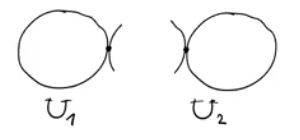
\includegraphics[width=0.4\linewidth]{images/topologia_algebrica/bouquet-circle-fundamental-group}
		\caption{}
		\label{fig:bouquet-circle-fundamental-group}
	\end{figure}
	Possiamo usare il teorema dei CW-complessi per retrarre $U \sim \S^1$ e $V \sim \S^1$, mentre l'intersezione è retraibile in un punto. Quindi diventa che 
	\begin{equation*}
		\pi_1(\S^1 \lor \S^1, x_0) \simeq \left\langle \alpha, \beta \mid \varnothing \right\rangle \simeq \Z \ast \Z
	\end{equation*}
\end{proof}

\begin{xca}
	Dimostriamo il seguente isomorfismo $\pi_1(T_1, x_0) \simeq \Z^2$
\end{xca}
\begin{proof}
	Prendiamo come suddivisione del toro gli aperti $U_1, U_2$ dove $U_1$ è il toro tolto un punto $Q$, mentre $U_2$ è il toro tolto i lati perimetrici che vengono incollati per costruire il toro (si veda la figura)
	\begin{figure}[h]
		\centering
		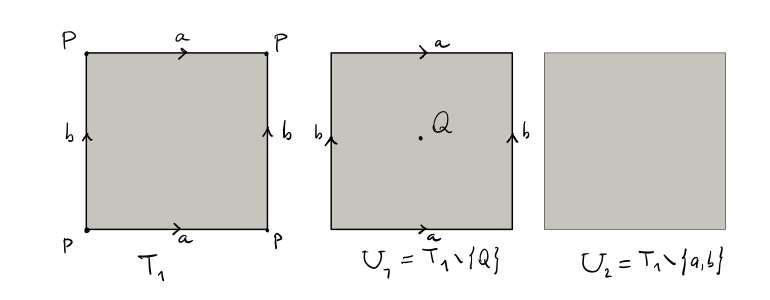
\includegraphics[width=0.7\linewidth]{images/topologia_algebrica/fundamental-group-torus}
		\caption{}
		\label{fig:fundamental-group-torus}
	\end{figure}
	Allora sappiamo che $\pi_1(U_1,x_0) \simeq \pi_1(\S^1 \lor \S^1, x_0) \simeq \Z \ast \Z$, mentre $U_2$ è contraibile (è essenzialmente un disco aperto). L'intersezione $U_1 \cap U_2$ invece è omotopicamente equivalente a $\S^1$, infatti se il buco si può allargare fino ad ottenere $\S^1$. Per cui otteniamo i seguenti risultati
	\begin{align*}
		\pi_1(U_1) & \simeq \Z \ast \Z \\
		\pi_1(U_2) & \simeq \Z_1 \\
		\pi_1(U_1 \cap U_2) &\simeq \Z \\
	\end{align*}
	poiché $\pi_1(U_1 \cap U_2)$ non è banale dobbiamo vedere quale è la relazione $R_{U_1 \cap U_2}$. Per vedere come interagisce sui cappi, dobbiamo ossservare che ogni cappio $c \in \pi_1(U_1 \cap U_2)$ può essere portato sul bordo di $U_1$ e, ciascuno dei cappi $c$ percorre i lati del toro in senso $aba^{-1}b^{-1}$, questo coincide alla relazione sui cappi di $\pi_1(U_1)$: $a \ast b \ast a^{-1} \ast b^{-1} = 1$ (si veda figura)
	\begin{figure}[h]
		\centering
		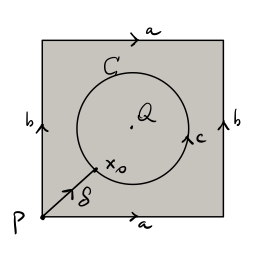
\includegraphics[width=0.4\linewidth]{images/topologia_algebrica/fundamental-group-torus-2}
		\caption{}
		\label{fig:fundamental-group-torus-2}
	\end{figure}	
	per cui diventa
	\begin{equation*}
		\pi_1(U_1 \cup U_2, x_0) \simeq \left\langle \{\alpha, \beta\} \cup \varnothing \mid R_{U_1 \cap U_2} \right\rangle \simeq \left\langle \alpha, \beta \mid \alpha \beta = \beta \alpha \right\rangle \simeq \Z^2
	\end{equation*} 
\end{proof}

\begin{xca}
	Dimostrare per ragionamento analogo a quello del toro che 
	
	\begin{equation*}
		\pi_1(U_h, x_0) \simeq \left\langle \alpha_1, \dots, \alpha_h \mid \alpha^2_1 \cdots \alpha^2_h = 1\right\rangle
	\end{equation*}.
\end{xca}
\begin{proof} Versione breve: \\
	Lo spazio proiettivo reale $U_1$ si costruisce come disco chiuso con due archi di circonferenza identificati. Prendo $V_1$ e $V_2$ esattamente come nel toro:
	\begin{itemize}
		\item $V_1$ è un bouquet di una circonferenza, di generatore $\alpha$
		\item $V_2$ è contraibile
		\item L'intersezione si retrae con deformazione su una circonferenza, dico $\delta$ il generatore di questa circonferenza
	\end{itemize}
	Siccome sono connessi per archi posso ragionare come sempre con il teorema di van Kampen ed ottengo (dato $sigma$ il solito cammino):
	\begin{equation*}
	[\delta]=\begin{cases}
	[\sigma \alpha^2 \sigma^{-1}]=[\sigma \alpha \sigma^{-1}]^2=A^2 & \text{ in $V_1$}\\
	1 & \text{ in $V_2$}
	\end{cases}
	\end{equation*}
	Quindi si vede che il gruppo fondamentale dello spazio proiettivo reale ha forma
	\begin{equation*}
	\pi(U_1,x)=\left\langle A \ | A^2 = 1 \right\rangle 
	\end{equation*}
\end{proof}

%todos: 0

\chapter{Varietà}


\newpage
\section{Le varietà topologiche}
\subsection{\textcolor{TopAlg}{\textbf{Introduzione allo studio delle varietà}}}

\begin{definition}
	Un $(X,\tau)$ spazio topologico, è detto \textbf{localmente euclideo} se per ogni $x \in X$ esiste $n \in \N$ e $U_x \subset X$ intorno aperto di $x$ tale che esiste un omeomorfismo $\morphism{\varphi_x}{U_x}{\mathring{\D}^n}$.  
\end{definition}

\begin{definition}
	Dato uno spazio topologico localmente euclideo, la coppia omeomorfismo intorno $(U_x, \varphi_x)$ è detta \textbf{carta locale}.
\end{definition}

\begin{remark}
	Dati due intorni distinti di $x$ per cui esiste una carta locale $(V_x, \varphi_x)$ e $(U_x, \psi_x)$, allora entrambi gli omeomorfismi avranno come codominio uno stesso $\mathring{\D}^n$ dove $n$ è uguale per entrambe le carte. (È un teorema profondo come un pozzo che non verrà trattato in queste note)
\end{remark}

\begin{theorem}
	Il disco nella topologia euclidea $\mathbb{D}^n$ è connesso per archi. 
\end{theorem} 
\begin{proof}
	Dimostro che il disco è convesso e quindi connesso per rette (e in particolare per archi). Infatti sia 
	\begin{equation}
	\mathbb{D}^n := \{x\in \R^n\; |\; |x| \le 1\}
	\end{equation}
	allora basta far vedere che presi due punti vale che l'intera retta sta nel disco. Siano $x, y \in \mathbb{D}^n$ allora
	\begin{equation}
	|(1-t)x+ty| \le (1-t)|x| + t|y| \le 1-t+t =1
	\end{equation}
	per cui stanno tutti nel disco, segue immediatamente la tesi. 
\end{proof}

\begin{remark}
	Dal teorema precedente si può notare perché si è scelto in particolare $\mathbb{D}^n$ come insieme di riferimento per le carte locali. Infatti questo insieme è abbastanza semplice, con una topologia abbastanza conosciuta, e ha proprietà che non tutti i sottospazi di $\R^n$ hanno (per esempio $\left[0,1\right] \cup (2,3)$ non è omeomorfo al disco, non è compatto, non è neanche connesso).
\end{remark}

\begin{definition}
	Se $X$ è una varietà topologica $n$ è detta la sua dimensione locale in $x$ e viene indicata dalla funzione
	\begin{equation}
	\begin{aligned}	
	\dim_x	\colon & X \rightarrow \N \\
	& 	x	\mapsto n \\
	\end{aligned}
	\end{equation}
\end{definition}

\begin{definition}
	La funzione $\dim_x$ è continua in $\N$ dotato della topologia discreta in quanto localmente costante. Inoltre se $X$ è compatto $\dim_x(X)$ dev'essere connesso e nella topologia discreta gli unici connessi sono i singoletti. Pertanto $\dim_x$ è costante se $X$ connesso.
\end{definition}

\begin{corollary}
	Se $X$ localmente euclideo e connesso, allora $\dim_x = k$ per qualche $k \in \N$. $k$ viene detta dimensione reale di $X$.
\end{corollary}

\begin{theorem}
	Sia $X$ localmente euclideo, allora $X$ è connesso per archi. 
\end{theorem} 
\begin{proof}
	Fisso un $x \in X$ e definisco 
	\begin{equation}
	W_x := \{z \in X \;|\; z \sim x\}
	\end{equation}
	dove $\sim$ è la relazione di essere connessi per archi. Innanzitutto notiamo che: 
	se $z \in W_x$ allora anche l'intorno $U_z$ è connesso per archi poiché localmente euclideo (basta passare per l'omeomorfismo locale).\\
	
	Per cui supponiamo che $W_x \neq X$ allora deve esistere almeno un $y \in X$ tale che non è in $W_x$. Distinguiamo due casi: 
	\begin{enumerate}
		\item Se $U_y \cap W_x \neq \varnothing$ allora posso usare la seconda osservazione per concludere che anche $y \in W_x$ contro l'ipotesi originaria, quindi $W_x = X$.
		\item Se $U_y \cap W_x = \varnothing$ allora dev'essere che $U_y \subset W^c_x$. Poiché per ogni punto di $W^c_x$ vale che il suo intorno sta in $W^c_x$ (se no avrei la possibilità di collegarli per archi con $x$) e quindi $W^c_x$ è aperto e $W_x$ chiuso. Inoltre sempre per l'osservazione iniziale $W_x$ dev'essere aperto. Poiché $X$ connesso dev'essere che $W_x = \varnothing$ (ma è impossibile perché $x\in W_x$) o $W_x = X$, ovvero la tesi. 
	\end{enumerate}
\end{proof}


\begin{theorem}
	Se $X$ localmente euclideo allora le sue componenti connesse sono aperte e chiuse.
\end{theorem}
\begin{proof}
	Se $X$ è connesso allora ha una sola componente connessa e quindi è sia chiusa che aperta.
	Sia $X$ sconnesso allora prendo una componente connessa $\left[x\right]_\sim$. Osservo che $\pi^{-1}(\left[x\right]_\sim)$ è un aperto: prendo un intorno $U_x \simeq \mathbb{D}^n$ per qualche $n$ e questo è connesso, per cui per ogni punto $x \in U_x \subset \pi^{-1}(\left[x\right]_\sim)$. Inoltre $\pi(\pi^{-1}(\left[x\right]_\sim)) = \left[x\right]_\sim$ per suriettività. Inoltre anche $\pi^{-1}(\left[x\right]^c_\sim)$ è aperto, infatti se fosse chiuso avrei che per ogni $y$ sulla frontiera questo sarebbe connesso con $x$, il ché sarebbe assurdo. Quindi $\left[x\right]_\sim$ è sia aperto che chiuso in $\tau_\sim$.
\end{proof}

\begin{remark}
	In generale se uno spazio topologico è localmente euclideo non è di Hausdorff. Infatti si consideri $\{a,b\} \times \R$ con la relazione di equivalenza $(x,y) \sim (z,w) \leftrightarrow y = w \land y > 0 \lor (x,y) = (z,w)$. Allora il disegno diventa una sorta di Y, in cui dove le due rette si congiungono c'è lo $0$ (che non viene identificato! ci sono due zeri: $\{0\}\times \{a\}, \{0\}\times \{b\}$).
	\begin{figure}[H]
		\centering
		
\includegraphics[width=0.35\linewidth]{images/topologia_generale/lcleucnott2}
		\caption{}
		\label{fig:lcleucnott2}
	\end{figure}
	
	Questo spazio è localmente euclideo (ricopri una retta alla volta e la parte unita la metti in entrambe le carte), ma non è di Hausdorff. Infatti prendiamo un intorno di $(0,a)$ denominiamlo $U$ e poi un intorno $V$ di $(0,b)$, questi si intersecheranno sempre sulla parte identificata delle due rette, per cui i due punti non rispettano la condizione di Hausdorff. 
	
	\begin{figure}[H]
		\centering
		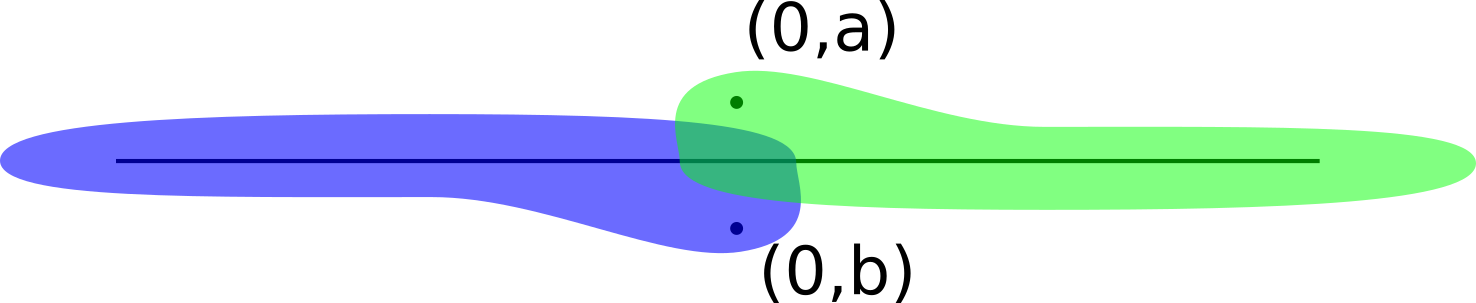
\includegraphics[width=0.7\linewidth]{images/topologia_generale/bug_eye}
		\caption{L'esempio della retta con due origini, con un possibile ricoprimento con due carte locali}
		\label{fig:bugeye}
	\end{figure}
	
	Un altro esempio è dato dalla linea con due origini che è molto simile all'esempio precedente, l'unica differenza è che si identificano tutte le rette tranne l'origine al posto che solo la parte positiva come avveniva sopra. Si prenda $\R \times \{a,b\}$ come spazio e si quozienti con la relazione $(x,a) \sim (y,b) \Longleftrightarrow x = y \land x,y \neq 0$. Allora lo spazio quoziente sarà dato da due rette distinte, ma con due origini $\{0\} \times \{a\}, \{0\}\times \{b\}$. Se si prende un qualsiasi intorno di $\{0\}\times \{a\}$ si avrà un intersezione per qualsiasi intorno di $\{0\} \times \{b\}$ per ovvie ragioni, per cui non è Hausdorff, malgrado sia localmente euclideo. Infatti basta prendere una carta locale di due mappe che cartografano $(-\infty, a) \cup \{0\}\times \{a\}$ e una che prende $(-a, +\infty) \cup \{0\}\times \{b\}$.  
\end{remark}

\subsection{\textcolor{TopAlg}{\textbf{Struttura delle varietà topologiche}}}
\begin{definition}
	Uno spazio topologico $(X,\tau)$ è detto \textbf{varietà topologica} di dimensione $n$ se è localmente euclideo, connesso, di Hausdorff e a base numerabile.
\end{definition}

\textbf{Alcuni esempi}

\begin{enumerate}
	\item Per $n=1$ le uniche varietà topologiche sono $\S^1$ e $\R$.
	\item Per $n=2$ le varietà topologiche si chiamano superfici topologiche e sono \textit{troppe}.
	\item Il toro si può costruire come $\left[0,1\right]^2/\Z^2$ si vede che è localmente euclideo, di Hausdorff, connesso e a base numerabile ed è anche compatto. Il toro è anche un esempio di superficie non orientabile e questo è di grande importanza nella teoria dei modelli minimali. Infatti grazie al toro è possibile generare tutte le superfici topologiche non orientabili. In generale il toro si indica con $T_g$ dove $g$ indica quante volte è stato aggiunto a  se stesso. Ad esempio un toro semplice si indica con $T_1$, mentre un bitoro $T_2$, mentre $T_0$ equivale alla sfera (più che altro per semplificare la notazione dei teorem, visto che è un caso limite).
	\item Anche il piano proiettivo si può esprimere come $\S^2 / \sim$ dove $a \sim b \Leftrightarrow a = rb$ per qualche $r \in \R$. Ma quest'ultimo si può vedere che è omeomorfo a $\D^2$. Pertanto $\mathbb{P}^2(\R) \simeq \D^2$. Il piano proiettivo viene denominato anche $U_n$ dove $n$ rapprensenta il numero di volte che viene sommato a se stesso, ovvero $U_1 + \dots + U_1 = U_n$.
\end{enumerate}

\begin{definition}[Somma connessa]
	Date due varietà topologiche $V_1, V_2$ è possibile trovare un intorno di $V_1$ e $V_2$ tali che sono omeomorfi (passando per la proiezione sul disco euclideo), per cui collegando le rispettive frontiere è possibile \textit{attaccare} $V_1$ con $V_2$. In particolare questa operazione si indica con $V_1 + V_2$ ed è indipendente dalla scelta dell'intorno a meno di omeomorfismi. 
\end{definition}


\begin{theorem}[Teorema di classificazione]
	Ogni superficie topologica compatta è omeomorfa a un $T_g$ per qualche $g \ge 0$ e $U_h$ per qualche $h \ge 1$, inoltre i due modelli non sono omeomorfi e sono minimali. 
\end{theorem}

L'intuizione di ciò è data dal fatto che il toro può essere rappresentato dalla stringa $aba^{-1}b^{-1}$ e il piano proiettivo da $aa$, mentre la sfera da $aa^{-1}$, per cui tutte le possibili stringhe sono di questo tipo visto che la somma connessa risulta essere, in questo caso, una semplice concatenazione di queste stringhe. La dimostrazione della minimalità verrà data nella prossima sezione.


\newpage
\section{Classificazione delle superfici compatte}
\subsection{\textcolor{TopAlg}{\textbf{Alcuni cenni di teoria dei gruppi}}}

Per poter classificare le superfici abbiamo bisogno di alcuni strumenti algebrici sui gruppi. In particolar modo il calcolo degli abelianizzati e dei gruppi dei nostri modelli fondamentali: il toro e il piano proiettivo.

\begin{lemma}
	\label{lemm:abel_torus_proj}
	Valgono i seguenti isomorfismi di gruppi
	\begin{equation}
	\begin{aligned}
	 Ab(\pi_1(U_h, x_0)) & \simeq \Z^{h-1} \times \Z_2 \\
	 Ab(\pi_1(T_g, x_0)) & \simeq \Z^{2g}
	\end{aligned}
	\end{equation}  
\end{lemma}
\begin{proof}[1]
	Sappiamo che $\pi_1(U_h) \simeq \left\langle \alpha_1, \dots, \alpha_h \mid \alpha^2_1 \cdots \alpha^2_h = 1\right\rangle$, quindi abelianizzando il gruppo si ottiene (utilizzando le trasformate di Tietze)
	\begin{equation}
	\begin{aligned}
		& Ab( \left\langle \alpha_1, \dots, \alpha_h \mid \alpha^2_1 \cdots \alpha^2_h = 1\right\rangle) \\
		& \simeq \left\langle \alpha_0, \alpha_1, \dots, \alpha_h \mid \alpha^2_1 \cdots \alpha^2_h = 1,\ \alpha_0 = \alpha_1 \dots \alpha_h,\ \left[a_i, a_j\right],\ \forall i,j \right\rangle\\
		& \simeq \left\langle \alpha_0, \alpha_1, \dots, \alpha_h \mid \alpha^2_0 = 1,\ \left[a_i, a_j\right],\ \forall i,j \right\rangle \\
		& \simeq \left\langle \alpha_1, \dots, \alpha_h \mid \left[a_i, a_j\right],\ \forall i,j \right\rangle \times \left\langle \alpha_0 \mid \alpha^2_0 = 1\right\rangle \simeq \Z^{h-1} \times \Z_2 
	\end{aligned}
	\end{equation}
\end{proof}
\begin{proof}[2]
	Sappiamo che $\pi_1(T_g) \simeq \left\langle \alpha_1, \dots, \alpha_g, \beta_1, \dots, \beta_g \mid \alpha_1 \beta_1\alpha^{-1}_1\beta^{-1}_1 \dots \alpha_g \beta_g\alpha^{-1}_g\beta^{-1}_g = 1\right\rangle$. Quindi la relazione sui generatori coincide al prodotto di tutti i commutatori, per cui 
	\begin{equation}
	\begin{aligned}
		& Ab(\left\langle \alpha_1, \dots, \alpha_g, \beta_1, \dots, \beta_g \mid \alpha_1 \beta_1\alpha^{-1}_1\beta^{-1}_1 \dots \alpha_g \beta_g\alpha^{-1}_g\beta^{-1}_g = 1\right\rangle) \\ & \simeq \left\langle \alpha_1, \dots, \alpha_g, \beta_1, \dots, \beta_g \mid \left[\alpha_1, \beta_1\right] = \dots \left[\alpha_g \beta_g\right] = 1\right\rangle\\
		& \simeq \left\langle \alpha_1 \mid \varnothing \right\rangle \times \dots \times \left\langle\beta_g \mid \varnothing \right\rangle \simeq \Z^{2g}
	\end{aligned}
	\end{equation}
\end{proof}

\begin{definition}
	Sia $G$ un gruppo abeliano; un elemento $g \in G$ si dice di torsione se per qualche $n \in \N$ vale $ng = 0$. L'insieme degli elementi di torsione forma il sottogruppo $T(G) \subset G$.
\end{definition}

\begin{lemma}
	Siano $G, G'$ gruppi abeliani. Allora valgono i seguenti fatti
	\begin{enumerate}
		\item Se $\morphism{\varphi}{G}{G'}$ è un morfismo tra gruppi, allora vale $\varphi(T(G)) \subseteq T(G')$.
		\item Se $\varphi$ come definito sopra è un isomorfismo, allora $\varphi|_{T(G)}$ un isomorfismo sui sottogruppi di torsione.
		\item Inoltre se $\varphi$ è un isomorfismo di gruppi, allora induce un isomorfismo $\morphism{\overline{\varphi}}{G/T(G)}{G'/T(G')}$.  
	\end{enumerate}
\end{lemma}

\begin{proposition}
	$\Z^n \simeq \Z^m$ se e solo se $m = n$. 
\end{proposition}
\begin{proof}
\end{proof}

\subsection{\textcolor{TopAlg}{\textbf{Il teorema di classificazione per le superfici compatte}}}
\begin{theorem}
	Sia $S$ una superficie compatta. Allora essa è omeomorfa a $T_g$ con $g\ge 0$ oppure ad una superficie $U_h$ per $h > 0$. Inoltre $T_g \not\simeq U_h$ per ogni $g,h$, $U_h \not\simeq U_{h'}$ per $h\neq h'$ e $T_{g'} \not\simeq T_g$ per $g \neq g'$.
\end{theorem}
\begin{proof}
	Il fatto che $S$ sia omeomorfa ad una delle due superfici è già stato dimostrato. Non resta che dimostrare la minimalità dei modelli presi.\\
	
	\textbf{$T_g \not\simeq U_h$}\\
	
	Consideriamo gli abelianizzati dei gruppi fondamentali rispettivi. Per il Lemma \ref{lemm:abel_torus_proj} vale che 
	\begin{equation}
	\begin{aligned}
		Ab(\pi_1(U_h, x_0)) & \simeq \Z^{h-1} \times \Z_2 \\
		Ab(\pi_1(T_g, x_0)) & \simeq \Z^{2g}
	\end{aligned}
	\end{equation}
	che hanno rispettivamente come sottogruppo di torsione $\Z_2$ e $\{0\}$, quindi non possono essere isomorfi ed in particolare non $T_g \not\simeq U_h$ (inoltre non sono neanche omotopicamente equivalenti).
	
	\textbf{$U_h \not\simeq U_{h'}$} \\
	
	Se fossero isomorfi allora gli abelianizzati sarebbero isomorfi e inoltre il quoziente dell'abelianizzato per il sottogruppo di torsione sarebbe isomorfo. In particolare 
	\begin{equation}
	\begin{aligned}
		\Z^{h-1} \simeq \Z^{h-1} \times \Z_2 / \Z_2 \simeq \Z^{h'-1} \times \Z_2 / \Z_2 \simeq \Z^{h'-1}
	\end{aligned}
	\end{equation}
	che funziona se e solo se $h = h'$.
	
	\textbf{$T_g \not\simeq T_{g'}$} \\
	
	Se fossero isomorfi allora gli abelianizzati sarebbero isomorfi quindi valrebbe $\Z^{2g} \simeq \Z^{2g'}$ che è valido solo se $g = g'$.
\end{proof}


% TODO: Inserire esempi da minuto 22 della lezione del 24/03/2020.

\begin{remark}
	Ricordiamo che affinché un retratto $\morphism{i}{A}{B}$ sia tale è necessario che $\morphism{i_*}{\pi(A, a)}{\pi(B, b)}$ sia un omomorfismo iniettivo; se vogliamo che sia un retratto di deformazione allora $i_*$ dev'essere un isomorfismo. 
\end{remark}

\begin{example}\
	\begin{enumerate}
		\item Siano $\S^1$ e $\D^2$ è ovvio che $\S^1$ non è un retratto di $\D^2$ dato che
		\begin{equation*}
		\pi(\S^1, x_0) \simeq \Z \not\subset \{1\} \simeq \pi(\D^2, x_0)
		\end{equation*}
		e quindi non può esistere una mappa iniettiva tra i due gruppi. 
		\item Si consideri $T_1$ come in figura.
		\begin{figure}[H]
			\centering
			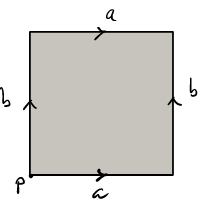
\includegraphics[width=0.3\linewidth]{images/topologia_algebrica/torus_polygon}
			\caption{}
			\label{fig:toruspolygon}
		\end{figure}
		Allora se si prende $A = \{a\}$, questo sarà un retratto di $T_1$, e vale
		\begin{equation*}
			\pi(A) \simeq \Z \hookrightarrow \Z^2 \simeq \pi(T_1)
		\end{equation*}
		analogamente vale per $A = \{b\}$.
		\item Sia $K$ una bottiglia di Klein con il poligono fondamentale come in figura. Osserviamo che $a, b$ hanno ruoli differenti. 
		\begin{figure}[H]
			\centering
			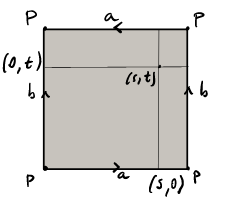
\includegraphics[width=0.3\linewidth]{images/topologia_algebrica/klein_polygon}
			\caption{}
			\label{fig:kelinpolygon}
		\end{figure}
		Infatti $B = \{b\}$ è un retratto della bottiglia di Klein, mentre $A = \{a\}$ non lo è. \
		
		Possiamo costruire un retratto per $B$: 
		\begin{equation*}
			r(\left[s,t\right]) = \left[0,t\right]
		\end{equation*}
		e osserviamo che è continua e ben definita e tale che $K \overset{r}{\hookrightarrow} B$.\
		
		Mostriamo che $A$ non è un ritratto. Prendiamo i gruppi fondamentale di $A$ e $K$ 
		\begin{equation*}
			\pi(K, P) \simeq \left\langle \alpha, \beta \,\middle|\, \alpha\beta\alpha\beta^{-1} = 1 \right\rangle \quad\ \pi(A, P) \simeq \left\langle \alpha \,\middle|\, \varnothing \right\rangle
		\end{equation*}
		supponiamo per assurdo che esista una retrazione $\morphism{r}{K}{A}$. Allora consideriamo le mappe indotte sui rispettivi gruppi fondamentali. Per cui
		\begin{equation*}
			r_*(\beta) \in \pi(A, P) \Longrightarrow \exists k \in \N \; \text{t.c.}\ r_*(\beta) = \alpha^k
		\end{equation*}
		per cui osserviamo che 
		\begin{equation*}
			 1 = r_*(1) = r_*(\alpha\beta\alpha\beta^{-1}) = \alpha\alpha^k\alpha\alpha^{-k} = \alpha^2
		\end{equation*}
		che contraddice le relazioni $\pi(A, P)$ quindi $A$ non è una retrazione di $K$. 		
	\end{enumerate}
\end{example}

%todos: 0



\part{Analisi Complessa}
\chapter{Calcolo differenziale}

\section{Differenziabilità in senso complesso}

Partiamo dal presupposto che possiamo identificare $\C$ con $\R^2$ dato che hanno la stessa topologia - e noi siamo interessati principalmente a questa struttura, dato che vogliamo definirne continuità e  differenziabilità in senso complesso. \\ Allora ogni funzione di una variabile complessa $\morphism{f}{\C}{\C}$ sarà essenzialmente trattata come se fosse una funzione $\morphism{f}{\R^2}{\R^2}$, ovvero ponendo $z = x + iy$
\begin{equation}
	f(z) = u(x,y) + iv(x,y)
\end{equation}
ma bisogna ricordare che le proprietà di $i$ ci daranno delle condizioni ulteriori sui criteri per cui possiamo definire $u, v$ e quindi ciò che diremo sui complessi non si potrà estendere direttamente sulle funzioni del tipo $\R^2 \to \R^2$. Possiamo comunque notare che $f$ è continua se e solo se $u,v$ lo sono (per proprietà universale del prodotto topologico).\\

Come nel caso reale in una variabile, possiamo esprimere la differenziabilità in funzione del limite del rapporto incrementale

\begin{definition}
	Sia $z \in \Omega \subset \C$. La funzione $f$ si dice \textbf{differenziabile} se esiste un numero complesso $f'(z)$ tale che per $h \to 0$ vale la seguente relazione
	\begin{equation}
		f(z+ h) - f(z) = f'(z)h + o(|h|)
	\end{equation} 
\end{definition}

\begin{definition}
	Sia $z \in \Omega \subset \C$. Se $f$ è differenziabile, la \textbf{derivata direzionale} di $f$ lungo $v \in \C$ (con $|v| = 1$) si definisce come
	\begin{equation}
		D_v f(z) = \lim_{r \to 0} \frac{f(z + rv) - f(z)}{r} = f'(z) v
	\end{equation}
\end{definition}


Inoltre, per come è stata definita la derivata, possiamo sfruttare tutte le proprietà che valgono nel caso reale di una variabile. Mostriamo alcuni esempi, come la derivata delle seguenti funzioni (se sono differenziabili \dots). \\

	\begin{equation*} \begin{aligned}
	f(z) & = \log(|z|)   \\
	f(z) & = e^{iz - |z|}  \\
	f(z) & = (1 + i - z)z^2  \\
	\end{aligned} \end{equation*}
\\

Occupiamoci della derivabilità in senso complesso: la seguente definizione è fondamentale.

\begin{definition}
	Una funzione $\morphism{f}{\Omega \subset \C}{\C}$ è detta \textbf{olomorfa} se è differenziabile in ogni $z \in \Omega$. \\ In generale indicheremo l'insieme delle funzioni olomorfe su $\Omega$ con $\mathcal{O}(\Omega)$.
\end{definition}

\begin{remark}
	Ogni funzione olomorfa è continua. Per dimostrarlo basta rispolverare la dimostrazione fatta nel caso dell'analisi reale.
\end{remark}

In virtù della relazione stabilità precedentemente, ovvero che $f = u + iv$ per degli $\morphism{u,v}{\R^2}{\R}$, otteniamo una condizione che ci eravamo limitati solo a ipotizzare.

\begin{theorem}[Equazioni di Cauchy-Riemann]
	Sia data una funzione complessa su $\Omega \subset \C$ del tipo $f(x+iy) = u(x,y) + iv(x,y)$ . Allora $f$ è differenziabile in $z \in \Omega$ se e solo se $u,v$ sono differenziabili e $u_x = v_y, u_y = - v_x$ (in $z \in \C$).
\end{theorem}
\begin{proof}
	Supponiamo $f$ differenziabile in $z=x+iy$. Allora consideriamo le derivate direzionali lungo l'asse reale e quello immaginario.
		\begin{equation*} \begin{aligned}
		D_{1} f  &= f'(z) = f_x(z) \\
		D_{i} f  &= f'(z)i = f_y(z)  
		\end{aligned}\end{equation*}
	dove $f_x(z) = u_x(x,y) + iv_x(x,y)$ e $f_y(z) = u_y(x,y) + iv_y(x,y)$. Da questo noto che vale la relazione
	\begin{equation*}
		f'(z) = u_x(z) + iv_x(x,y) = -i(u_y(x,y) + iv_y(x,y))
	\end{equation*}	
	ovvero $u_x(x,y) = v_y(x,y), v_x(x,y) = -u_y(x,y)$. Inoltre ci serve osservare che $u,v$ sono differenziabili in $z$: infatti poiché $f$ è differenziabile, allora anche la sua parte reale è differenziabile, come anche la sua parte immaginaria, e per $h = a + ib$ vale dunque 
	\begin{equation*}
	\begin{aligned}
		u(z+h) - u(z) & = u_x a - v_x b + o(\sqrt{a^2 + b^2})\\
		v(z+h) - v(z) & = u_x b + v_x a + o(\sqrt{a^2 + b^2})
	\end{aligned}
	\end{equation*}
	ovvero $u,v$ sono differenziabili in $z$, che era quanto si voleva dimostrare. 
	Supponiamo quindi che $u,v$ siano differenziabili in $z$ e valgano le relazioni sopra descritte. Allora con qualche calcolo si ottiene, sempre per $h = a + ib$
	\begin{equation*}
	\begin{aligned}
		u(z+h) - u(z) & = a u_x(z) + b u_y(z) + o(|h|) = a u_x(z) - b v_x(z) + o(|h|) \\
		v(z+h) - v(z) & = a v_x(z) + b v_y(z) + o(|h|) = a v_x(z) + b u_x(z) + o(|h|) \\
		\end{aligned}
	\end{equation*}
	da cui - ricordando la definizione di $f$ - si ottiene direttamente che questa è derivabile in senso complesso.
\end{proof}

\begin{corollary}
	La matrice delle funzioni reali $\morphism{(u,v)}{\Omega \subset \R^2}{\R^2}$ tali da descrivere una funzione complessa $f$, sono tali che  
	\begin{equation*}
	\begin{aligned}
		J_{(u,v)} = \left( \begin{array}{cc}
					u_x & - v_x\\ v_x & u_x
					\end{array} \right)
	\end{aligned}
	\end{equation*}
	In particolare il determinante è $\det J_{(u,v)} = u^2_x + v^2_x \ge 0$.
\end{corollary}

\begin{corollary}
	Se $f'(z) = 0$, $f$ è una funzione costante.
\end{corollary}

\begin{corollary}
	Se $f = u + iv$ con $u(x,y) = r \in \R$ e $f \in C^1$, allora 
	\begin{equation*} \begin{aligned}
	0 = u_x &= v_y \\
	0 = u_y &= -v_x
	 \end{aligned}\end{equation*}
	 (cioè $f' = 0$, dunque $f$ è una funzione costante). \\ Viceversa se $v(x,y) = p \in \R$ allora $f$ è una funzione costante.   
\end{corollary}

\section{Funzioni armoniche, operatori di Wirtinger}

\begin{definition}[Operatori di Wirtinger]
	Sia $\morphism{f}{\Omega}{\C}$ funzione di classe $C^1(\Omega)$. Allora possiamo definire i seguenti operatori
	\begin{equation}
	\begin{aligned}
		\frac{\partial f}{\partial z} := \frac{1}{2}(f_x - if_y) \quad\ \frac{\partial f}{\partial \overline{z}} := \frac{1}{2}(f_x + if_y)
	\end{aligned}
	\end{equation}
\end{definition}

\begin{remark}
	Si dimostra che una funzione soddisfa il teorema di Cauchy-Riemann sse vale 
	\begin{equation*}
		\frac{\partial f}{\partial \overline{z}} = 0
	\end{equation*}
	In particolare se $f$ olomorfa 
	\begin{equation*}
		\frac{\partial f(z)}{\partial z} = f'(z) 
	\end{equation*}
\end{remark}

\begin{remark}
	Se $f \in C^1(\Omega)$, allora soddisfa le equazioni di Cauchy-Riemann. In particolare se supponiamo $f = u+iv$ ulteriormente derivabile - cosa che non è necessario supporre, dato che le funzioni olomorfe, come vederemo in seguito, sono $C^\infty$ - possiamo costruire una relazione sulle funzione $u,v$:
	\begin{equation*}
	\begin{aligned}	
		u_{xx} & = (v_y)_x = (v_x)_y = (-u_y)_y = u_{yy} \\
		v_{xx} & = (-u_y)_x = -(u_x)_y = -(v_y)_y = -v_{yy}\\
	\end{aligned}
	\end{equation*}
	ovvero le due funzioni reali sono \textbf{armoniche}, dato che hanno operatore laplaciano nullo. In generale vale il seguente enunciato (che verrà dimostrato in seguito):\\
	
	\textit{Sia $\morphism{u}{\Omega \subset \R^2}{R}$ una funzione armonica su un dominio semplicemente connesso $\Omega$. Allora esiste una funzione armonica $\morphism{v}{\Omega}{\R}$ - unica a meno di una costante - tale che $f(z=x+iy) = u(x,y) + iv(x,y)$ sia una funzione olomorfa}.
\end{remark}		
	
\section{Funzioni analitiche o funzioni olomorfe?}

Il termine \textit{analitico} si perde nel contesto delle funzioni complesse dato che, come vedremo, l'insieme delle funzioni olomorfe coincide con quello delle funzioni analitiche. \\ Pertanto si preferisce descrivere le funzioni analitiche come olomorfe - una condizione facilmente accertabile, data anche l'equivalenza stabilita delle equazioni di Cauchy-Riemann. \\ \\ In questa sezione ci limiteremo a sviluppare la teoria strettamente necessaria per stabilire la convergenza di serie complesse, arrivando infine a dimostrare quanto detto sfruttando il teorema di Abel.\\

\begin{definition}
	\label{defn:successione-di-funzioni-complesse}
	Sia $\Omega \subset \C$ e sia $\{f_n\}_{n\in\N}$ con $\morphism{f_n}{\Omega}{\C}$ funzione, allora $\{f_n\}_{n\in\N}$ si dice \textbf{successione di funzioni complesse}.
\end{definition}

\begin{definition}
	\label{defn:serie-di-funzioni-complesse}
	Data una successione di funzioni complesse $\{f_n\}_{n\in\N}$ definite su $\Omega\subset\C$, allora 
	\begin{equation}
	\begin{aligned}
		\sum_{n=0}^{+\infty} f_n 
	\end{aligned}
	\end{equation}
	si dice \textbf{serie di funzioni complesse}.
\end{definition}

\begin{definition}
	\label{defn:convergenza-puntuale-successione}
	Data una successione di funzioni complesse definite su $\Omega$, $\{f_n\}_{n\in\N}$, se per ogni $z \in \Omega$ vale 
	\begin{equation}
	\begin{aligned}
		f_n(z) \to f(z) \quad\ \text{per}\ n \to +\infty
	\end{aligned}
	\end{equation}
	per una qualche $\morphism{f}{\Omega}{\C}$, allora si dice che la successione \textbf{converge puntualmente} a $f$.
\end{definition}

\begin{definition}
	\label{defn:convergenza-puntuale-serie}
	Data una successione di funzioni complesse definite su $\Omega$, $\{f_n\}_{n\in\N}$, se per ogni $z \in \Omega$ vale 
	\begin{equation}
	\begin{aligned}
		\sum^{n}_{k=0} f_k(z) \to f(z) \quad\ \text{per}\ n \to +\infty
	\end{aligned}
	\end{equation}
	per una qualche $\morphism{f}{\Omega}{\C}$, allora si dice che la serie \textbf{converge puntualmente} a $f$.
\end{definition}

\begin{definition}
	\label{defn:convergenza-uniforme-successione}
	Data una successione di funzioni complesse definite su $\Omega$, $\{f_n\}_{n\in\N}$, se vale 
	\begin{equation}
	\begin{aligned}
		\sup_{z \in \Omega} |f_n(z) - f(z)| \to 0 \quad\ \text{per}\ n \to +\infty
	\end{aligned}
	\end{equation}
	per una qualche $\morphism{f}{\Omega}{\C}$, allora si dice che la successione \textbf{converge uniformemente} a $f$.
\end{definition}

\begin{definition}
	\label{defn:convergenza-uniforme-serie}
	Data una successione di funzioni complesse definite su $\Omega$, $\{f_n\}_{n\in\N}$, se vale 
	\begin{equation}
	\begin{aligned}
		\sup_{z \in \Omega} |\sum^{N}_{n=0}f_n(z) - f(z)| \to 0 \quad\ \text{per}\ N \to +\infty
	\end{aligned}
	\end{equation}
	per una qualche $\morphism{f}{\Omega}{\C}$, allora si dice che la serie \textbf{converge uniformemente} a $f$.
\end{definition}	
	
\begin{definition}
	\label{defn:convergenza-assoluta}
	Data una successione di funzioni complesse definite su $\Omega$, $\{f_n\}_{n\in\N}$, se per ogni $z \in \Omega$ vale 
	\begin{equation}
	\begin{aligned}
		\sum^{+\infty}_{n=0} |f_n|(z) < +\infty \quad\ \text{per}\ n \to +\infty
	\end{aligned}
	\end{equation}
	allora si dice che la serie \textbf{converge assolutamente}.	
\end{definition}

\begin{remark}
	Osserviamo infine che se una serie $\{\sum^n_{k=0}f_k\}_{n \in \N}$ è assolutamente convergente, allora è anche puntualmente convergente, infatti
	\begin{equation*}
		|\sum^n_{k=0} f_k(z)| \le \sum^n_{k=0} |f_k(z)| = l < +\infty
	\end{equation*} 
	per cui $\sum^n_{k=0} \Re(f_k(z)) < +\infty,\ \sum^n_{k=0} \Im(f_k(z)) < +\infty$. Per cui tutta la serie converge a qualche funzione $f$ in ogni punto.
\end{remark}

\begin{theorem}[M-test di Weierstrass]
	\label{thr:m-test-weierstrass} Sia $\{f_n\}_{n\in\N}$ una successione di funzioni complesse e $\{M_n\}_{n\in\N}$ una successione di numeri reali positivi per cui vale $|f_n(z)| \le M_n \forall z\in \Omega$. Se la serie 
	\begin{equation*}
		\sum_{n=0}^{+\infty} M_n < +\infty
	\end{equation*} 
	allora anche la serie 
	\begin{equation*}
		\sum_{n=0}^{+\infty} f_n(z)
	\end{equation*}
	converge assolutamente ed uniformemente in $\Omega$.
\end{theorem}
\begin{proof}
	Ovviamente che la serie converge in modo assoluto su tutto $\Omega$ per ipotesi. Allora cui definiamo $s_n(z) := \sum_{k=0}^n f_k(z)$ e $s$ la funzione a cui converge la serie. Allora
	\begin{equation*}
		|s - s_n| = \left|\sum_{k=n+1}^{+\infty} f_k\right| \le \sum_{k=n+1}^{+\infty} \left|f_k\right| \le \sum_{k=n+1}^{+\infty} M_k
	\end{equation*}
	Dato che la serie degli $M_k$ converge, fissato un qualsiasi $\varepsilon > 0$ possiamo sempre trovare $N$ tale per cui $\sum_{k>N} M_k < \varepsilon$. Per l'assoluta generalità con cui è stato scelto $z \in \Omega$ ottengo la tesi di uniforme convergenza. 
\end{proof}

\begin{definition}
	\label{defn:serie-di-potenze}
	Siano dati $z_0 \in \C$ e una successione $\{a_n\}_{n\in \N}$ di valori in $\C$, allora si definisce \textbf{serie di potenze} la serie della seguente forma
	\begin{equation*}
		S(z) := \sum_{n=0}^{+\infty} a_n(z-z_0)^n
	\end{equation*}
\end{definition}

\begin{theorem}[Criterio di Hadamard]
	\label{thr:criterio-hadamard}
	Data una serie di potenze $S$ con notazione come in Definizione \ref{defn:serie-di-potenze}, definiamo il suo\textbf{raggio di convergenza} come $R := ( \limsup_{n\to+\infty} \sqrt[n]{a_n})^{-1} \in \left[0,+\infty\right]$. Allora 
	\begin{enumerate}
		\item La serie di potenze $S$ converge assolutamente nel disco $B_{z_0}(R)$ e non converge per $z \notin \overline{B_{z_0}(R)}$.
		\item La serie di potenze converge su ogni disco chiuso $\overline{B_{z_0}(r)}$ con $r < R$.  
	\end{enumerate}
\end{theorem}
\begin{proof}
	Possiamo supporre $z_0 = 0$ - senza perdita di generalità, dato che basta effettuare una sostituzione per riportarci nel caso $z_0 = 0$ dato un qualsiasi $z_0 \in \C$.\\ 
	Dimostro che la serie di potenze converge uniformemente e assolutamente per ogni $0 < r < R$. Essendo $R < t^{-1}$ allora esiste un $N$ per cui
	
		\begin{equation*}
		\sqrt[n]{a_n} < t^{-1} \quad\ \text{per ogni}\ n \ge N 
		\end{equation*}
	
	dunque $|a_n| < t^{-n}$ per ogni $n \ge N$. \\ Se $|z| \le r$ vale
	
	\begin{equation*}
	|a_nz^n| < \left(\frac{r}{t}\right)^n
	\end{equation*}
	
	Per il Teorema \ref{thr:m-test-weierstrass} la serie di potenze converge $\forall z \in \Omega$ - dove $\Omega = B_0(r)$ - e siccome vale per ogni $r < R$ segue anche per $B_0(R)$.\\
	
	Dimostriamo ora che non converge da nessuna parte al di fuori della chiusura del disco aperto $\overline{B_{z_0}(R)}$. Infatti se supponessimo la convergenza in qualche punto $z \in \C \setminus \overline{B_{z_0}(R)}$ allora $|z| > R$ e $|z|^{-1} < R$. Per cui $\forall n \ge N$ con $N \in \N$ vale che
	
		\begin{equation*}
		|z|^{-1} < \sqrt[n]{|a_n|}
		\end{equation*}
		
	per cui otteniamo 
	\begin{equation*}	
	\sum^{+\infty}_{n=0}|z|^{-n}|z|^n = \sum^{+\infty}_{n=0}|\sqrt[n]{|a_n|}|^n|z|^n < \sum^{+\infty}_{n=0}|a_n||z^n| 
	\end{equation*}
	
	e la prima serie è ovviamente non assolutamente convergente per ogni $|z| > R$.
\end{proof}

\begin{theorem}
	\label{prop:invarianza-raggio-convergenza-derivata}
	Data una serie di potenze definiamo la sua derivata come 
	\begin{equation}
	\begin{aligned}
		S'(z) = \sum^{+\infty}_{k=1} ka_k(z-z_0)^{k-1}
	\end{aligned}
	\end{equation} 
	e dunque i raggi di convergenza di $S'$ ed $S$ sono gli stessi.
\end{theorem}
\begin{proof}
	È un ovvia applicazione del calcolo dei limiti; definiamo con $b_n = (n+1)a_{n+1}$ i coefficienti della serie di potenze derivata. 
	\begin{equation*}
	\begin{aligned}
		\limsup_{n\to+\infty} \sqrt[n]{b_n} & = \limsup_{n\to+\infty} \sqrt[n]{(n+1)a_{n+1}} \\
											& = \limsup_{n\to+\infty} \sqrt[n]{(n+1)} \sqrt[n]{a_{n+1}} \\
											& = \limsup_{n\to+\infty} \sqrt[n]{a_{n+1}} = \limsup_{n\to+\infty} \sqrt[n]{a_{n}} 
	\end{aligned}
	\end{equation*}
	che è appunto lo stesso raggio di convergenza.
\end{proof}

\begin{theorem}[Teorema di Abel]
	\label{thr:teorema-di-abel}
	Sia $S$ una serie di potenze con raggio di convergenza $R > 0$. Allora $S(z)$ è una funzione olomorfa in $|z-z_0| < R$ e $S'$ è la sua derivata.
\end{theorem}
\begin{proof}
	Assumiamo ancora una volta che $z_0$ della serie di potenze sia $z_0 = 0$. Prendiamo quindi $z \in B_0(R)$ e sia $\delta > 0$ tale che $\overline{B_0(\delta)} \subset B_0(R)$. Prendiamo quindi un $h \in B_0(\delta)$. Allora
	\begin{equation*}
	\begin{aligned}
		\frac{f(z+h) - f(z)}{h} & = \sum^{+\infty}_{n=0} a_n \frac{(z+h)^n - z^n}{h} = \sum^{+\infty}_{n=0} a_n \frac{(z+h)^n-z^n}{z+h-z} \\
								& = \sum^{+\infty}_{n=0} a_n z^{n-1} \frac{\left(\frac{z+h}{z}\right)^n - 1}{\left(\frac{z+h}{z}\right)^n - 1} \\
								& = \sum^{+\infty}_{n=0} a_n \sum^{n-1}_{j=0} z^{n-1-j}(z+h)^j 
	\end{aligned}
	\end{equation*}
	Vogliamo mostrare che la serie sopra descritta converge uniformemente.
	\begin{equation*}
		|z+h| \le |z| + |h| \le |z| + \delta
	\end{equation*}
	Quindi possiamo scrivere 
	\begin{equation*}
		\left|a_n \sum^{n-1}_{j=0} z^{n-1-j}(z+h)^j \right| \le n|a_n|(|z|+\delta)^{n-1} 
	\end{equation*}
	Utilizzando il Teorema \ref{thr:m-test-weierstrass} con $M_n = n|a+n|(|z|+\delta)^{n-1}$ sappiamo che converge per ogni $|z|+\delta < R$, dato che dal Teorema \ref{prop:invarianza-raggio-convergenza-derivata} vale che la derivata di una funzione ha lo stesso raggio di convergenza della funzione stessa. Per cui converge uniformemente in ogni $|z| < R$. 
	Possiamo quindi calcolare il limite del rapporto incrementale, da cui si ottiene 
	\begin{equation*}
		\lim_{h\to 0} \frac{f(z+h) - f(z)}{h} = \sum^{+\infty}_{n=1} na_nz^{n-1}
	\end{equation*}
\end{proof}

\begin{remark}
	Utilizzando il teorema di Abel posso mostrare che ogni funzione analitica è localmente olomorfa nel suo raggio di convergenza, ma per quanto abbiamo "previsto" precedentemente sappiamo anche che una funzione olomorfa è $C^\infty$, quindi potremmo sviluppare \textit{all'infinito} Taylor ed ottenere una serie di potenze localmente identiche alla funzione iniziale. \\ Concludiamo dunque con la notevole - ed importante! - osservazione che
	\begin{equation*}
	\begin{aligned}
		f \ \ \textrm{ANALTICA} \ \Longleftrightarrow \ f \ \  \mathrm{OLOMORFA}
	\end{aligned}
	\end{equation*}
\end{remark}

%todos: 0

\chapter{Integrali di linea}
Il corso si fonderà sul calcolo degli integrali di funzioni in variabile complessa su un dominio - o una curva - complesso: vedremo alcune definizioni ed alcuni teoremi per il calcolo integrale e noteremo come le curve abbiamo un ruolo fondamentale. Presto scopriremo anche come \enquote{scegliere} le curve per semplificare i calcoli. \\ \\ Ci inoltreremo nel teorema più importante di questa sezione del corso: il \textit{teorema integrale di Cauchy}.
\newpage
\section{Integrare su una curva}
\subsection{\textcolor{AnComp}{\textbf{Integrare su una curva}}}

Vogliamo definire l'integrale di funzioni complesse su curve nel piano complesso. Per fare ciò parametriziamo le curve complesse su un intervallo reale. 

\begin{definition}
	\label{defn:integrale-funzione-complessa-parametrizzata-su-intervallo-reale}
	Sia $\morphism{f}{\left[a,b\right]\subset \R}{\C}$ una funzione continua, siccome possiamo scrivere $f(t) = u(t)+ iv(t)$ allora vale che
	\begin{equation*}
	\begin{aligned}
	\int_{a}^{b} f(t)\ dt \coloneqq \int_{a}^{b} u(t)\ dt + i \int_{a}^{b} v(t)\ dt 
	\end{aligned}
	\end{equation*}
\end{definition}

\begin{proposition}
	\label{prop:proprieta-funzione-complessa-parametrizzata-su-intervallo-reale}
	Valgono le seguenti proprietà per l'integrale definito in Definizione \ref{defn:integrale-funzione-complessa-parametrizzata-su-intervallo-reale}
	\begin{enumerate}
		\item è lineare, infatti, per ogni $\lambda, \mu \in \C$ e $\morphism{f,g}{\left[a,b\right]}{\C}$ vale
		\begin{equation*}
		\begin{aligned}
		\int_{a}^{b} \lambda f(t)  + \mu g(t)\ dt = \lambda \int_{a}^{b} f(t)\ dt + \mu \int_{a}^{b} g(t)\ dt   
		\end{aligned}
		\end{equation*}
		\item commuta con l'operazione $\Re, \Im$.
		\begin{equation*}
		\begin{aligned}	
		\Re\left(\int_{a}^{b} f(t)\ dt\right) = \int_{a}^{b} \Re(f(t))\ dt \quad\ \Im\left(\int_{a}^{b} f(t)\ dt\right) = \int_{a}^{b} \Im(f(t))\ dt
		\end{aligned}
		\end{equation*} 
		\item vale la seguente disuguaglianza
		\begin{equation*}
		\begin{aligned}
		\left|\int_{a}^{b} f(t)\ dt\right| \le \int_{a}^{b} |f(t)|\ dt
		\end{aligned}
		\end{equation*}
		\item Se $\morphism{\theta}{\left[c,d\right]}{\left[a,b\right]}$ è di classe $C^1$ e ha un inversa di classe $C^1$ allora
		\begin{equation*}
		\begin{aligned}
		\int_{\theta(c)}^{\theta(d)} f(t)\ dt = \int_{a}^{b} f(\theta(t))\theta'(t)\ dt
		\end{aligned}
		\end{equation*}
	\end{enumerate} 
\end{proposition}
\begin{proof}[Dimostrazione di (1)]
	Il primo punto deriva dalla linearità dell'integrale di Riemann. 
	Basta dividere in parte reale e immaginaria della funzione $f = u+ iv$.
\end{proof}

\begin{proof}[Dimostrazione di (2)]
	Segue dalla linearità dividendo la funzione in parte reale e immaginaria.	
\end{proof}

\begin{proof}[Dimostrazione di (3)]
	Poniamo $\omega \coloneqq \int_{a}^{b} f(t)\ dt$, allora se $\omega = 0$ è dimostrata. Se $\omega \neq 0$ allora poniamo $u = \overline{\omega}/|\omega|$, osserviamo che $|u|=1$. Da cui
	\begin{equation*}
	\begin{aligned}
	|w| = uw = \int_{a}^b \Re(uf(t))\ dt \le \int_{a}^b |uf(t))|\ dt = \int_{a}^b |f(t))|\ dt  
	\end{aligned}
	\end{equation*}
\end{proof}

\begin{proof}[Dimostrazione di (4)]
	Questo si può vedere come la Formula dell'area  
	\begin{equation*}
	\begin{aligned}
	\int_{\theta(a,b)} f(z) dz & = \int_{\theta(a,b)} u(x,y) \mathcal{L}^2(x,y)
	+ i\int_{\theta(a,b)} v(x,y) \mathcal{L}^2(x,y)\\
	& = \int_a^b u(\theta(t))\theta'(t) \mathcal{L}^1(t) 
	+ i\int^b_a v(\theta(t))\theta'(t) \mathcal{L}^2(t)\\
	& = \int_a^b f(\theta(t)) \theta'(t)\ dt		
	\end{aligned}
	\end{equation*}
\end{proof}

\begin{definition}
	\label{defn:curva-c1}
	Una \textbf{curva di classe $C^1$} nel piano complesso è una funzione $\morphism{\gamma}{J=\left[a,b\right]}{\C}$ di classe $C^1$. L'immagine $\gamma(J) \subset \C$ è detta \textbf{traccia o sostegno della curva}. Una curva di classe $C^1$ a tratti è una funzione continua $\morphism{\gamma}{J}{\C^1}$, di classe $C^1$ su $J$ meno un numero finito di punti. 		
\end{definition}

\begin{definition}
	\label{defn:riparametrizzazione-curva-classe-c1}
	Sia $\morphism{\theta}{\left[c,d\right]}{\left[a,b\right]}$ una funzione di classe $C^1$, con inversa di classe $C^1$. Supponiamo che $\theta' > 0$ su $\left[c, d\right]$. Dunque $\theta$ è monotona crescente, con $\theta(c) = a$, $\theta(d) = b$. La curva di classe $C^1$ definita da $\morphism{\overline{\gamma}(s) = \gamma(\theta (s))}{\left[c,d\right]}{\C}$ è detta \textbf{riparametrizzazione di $\gamma$}.
\end{definition}

\begin{definition}
	\label{defn:lunghezza-di-curva-classe-c1}
	La \textbf{lunghezza} della curva di classe $C^1$ $\morphism{\gamma}{\left[a,b\right]}{\C}$ è definita come l'integrale 
	\begin{equation*}
	\begin{aligned}
	l(\gamma) \coloneqq \int_{a}^{b} |\gamma'(t)|\ dt
	\end{aligned}
	\end{equation*}
\end{definition}

\begin{definition}
	\label{defn:integrale-di-linea}
	Sia $\morphism{\gamma}{\left[a,b\right]}{\C}$ una curva di classe $C^1$ con sostegno contenuto in un aperto $\Omega \subset \C$. Sia $\morphism{f}{\Omega}{\C}$ allora
	\begin{equation*}
	\begin{aligned}
	\int_\gamma f(z)\ dz \coloneqq \int_{a}^b f(\gamma(t)) \gamma'(t) \ dt
	\end{aligned}
	\end{equation*}  
\end{definition}

\begin{remark}
	La definizione \ref{defn:integrale-di-linea} è dipendente dalla parametrizzazione utilizzata, ma ciò non toglie che dia, per parametrizzazioni che non cambiano l'orientazione della curva, lo stesso risultato (come si può riparametrizzando avanti e indietro la curva).
\end{remark}

\begin{proposition}
	\label{prop:proprieta-integrale-di-linea}
	L'integrale in Definizione \ref{defn:integrale-di-linea} ha le seguenti proprietà
	\begin{enumerate}
		\item è lineare, ovvero date $\morphism{f,g}{\Omega \subset \C}{\C}$ e $\lambda, \mu \in \C$ vale
		\begin{equation*}
		\begin{aligned}
		\int_{\gamma} \lambda f(z) + \mu g(z) \ dz =  \lambda \int_{\gamma} f(z) \ dz + \mu \int_{\gamma} g(z) \ dz 
		\end{aligned}
		\end{equation*}
		\item vale la seguente disequazione per ogni $\morphism{f}{\Omega}{\C}$
		\begin{equation*}
		\begin{aligned}
		\left|\int_{\gamma} f(z) \ dz\right| \le \max_{\gamma} |f(z)| \mathcal{H}^1(\gamma)	
		\end{aligned}
		\end{equation*}
		\item sia $-\gamma(t) \coloneqq \gamma(a+b-t)$ la curva percorsa in senso opposto a quello di $\gamma$, allora
		\begin{equation*}
		\begin{aligned}
		\int_{-\gamma} f(z) \ dz = - \int_{\gamma} f(z) \ dz
		\end{aligned}
		\end{equation*}
		\item Se esiste $F$ olomorfa tale che $F' = f$ su tutto $\Omega$ allora
		\begin{equation*}
		\begin{aligned}
		\int_\gamma f(z) \ dz = F(\gamma(b)) - F(\gamma(a))
		\end{aligned}
		\end{equation*}
		In particolare, se $\gamma$ è chiusa, vale $\int_\gamma f(z)\ dz = 0$.
	\end{enumerate}
\end{proposition}
\begin{proof}[1]
	Deriva immediatamente dal punto 1 della Proposizione \ref{prop:proprieta-funzione-complessa-parametrizzata-su-intervallo-reale}.
\end{proof}
\begin{proof}[2]	
	Segue dal punto $3$ della Proposizione \ref{prop:proprieta-funzione-complessa-parametrizzata-su-intervallo-reale}:
	\begin{equation*}
	\begin{aligned}
	\left|\int_\gamma f(z)\ dz\right| \le \int^b_a |f(\gamma(t))||\gamma'(t)| \ dt \le \max_{\gamma} f(z) \mathcal{H}^1(\gamma(\left[a,b\right])) 
	\end{aligned}
	\end{equation*}
\end{proof}
\begin{proof}[3]
	È conseguenza della formula $4$ della Proposizione \ref{prop:proprieta-funzione-complessa-parametrizzata-su-intervallo-reale}. Ponendo $s = \theta(t) = a + b - t$ si ottiene
	\begin{equation*}
	\begin{aligned}
	\int_{-\gamma} f(z)\ dz = \int_{\gamma(\theta))} f(z)\ dz = -\int_{\gamma} f(z)\ dz
	\end{aligned}
	\end{equation*}
\end{proof}
\begin{proof}[4]
	Osserviamo che $\odv{F \circ \gamma}{t} = (f \circ \gamma) \gamma'$. Per cui dal teorema fondamentale del calcolo integrale
	\begin{equation*}
	\begin{aligned}
	\int^b_a f(\gamma(t))\gamma'(t)\ dt = \int_a^b (F \circ \gamma)'(t)\ dt = F(\gamma(b)) - F(\gamma(a))
	\end{aligned}
	\end{equation*}
\end{proof}

\begin{remark}
	Le stesse proprietà valgono con opportuni accorgimenti anche per curve $C^1$ quasi ovunque. Infatti basta togliere i punti in cui non è definita la curva e considerare i tratti $C^1$. 
\end{remark}

\begin{theorem}
	Non esiste una funzione logaritmo olomorfa su tutto $\C \setminus \{0\}$.
\end{theorem}
\begin{proof}
	Osserviamo che se $\gamma(t) = e^{it} \colon \left[0,2\pi\right] \to \C$ allora $\gamma'(t) = ie^{it}$. Per cui
	\begin{equation*}
	\begin{aligned}
	\int_\gamma \frac{1}{z}\ dz = \int_{0}^{2\pi} \frac{1}{e^{it}} ie^{it}\ dt = 2i\pi
	\end{aligned}
	\end{equation*}
	
	Supponiamo esista $\morphism{f}{\C \setminus \{0\}}{\C}$ funzione logaritmo olomorfa su tutto il suo dominio. Allora $e^{f(z)} = z$ e quindi si avrebbe
	\begin{equation*}
	\begin{aligned}
	1 = z' =(e^{f(z)})' = e^{f(z)} f'(z) 
	\end{aligned}
	\end{equation*}
	ovvero $f'(z) = 1/z$. Quindi $f$ sarebbe una primitiva olomorfa di $1/z$. Quindi per il punto $4$ della Proposizione \ref{prop:proprieta-integrale-di-linea} si avrebbe che $\int_{\gamma} 1/z \ dz = 0$, contraddicendo l'osservazione fatta all'inizio. 
\end{proof}

\begin{theorem}[di Goursat]
	\label{thr:groursat}
	Sia $\Omega \subset \C$ un aperto, sia $f \in \mathcal{O}(\Omega)$ e sia $R$ un rettangolo tale che $R \subset \Omega$. Allora 
	\begin{equation*}
	\begin{aligned}
	\int_{\partial R} f(z)\ dz = 0
	\end{aligned}
	\end{equation*}
	ove $\partial R$ è il bordo del rettangolo (il perimetro) percorso in senso anti-orario.
\end{theorem}
\begin{proof}
	Per ogni rettangolo $R' \subset \Omega$ definiamo 
	\begin{equation*}
	\begin{aligned}
	\eta(R') \coloneqq \left| \int_{\partial R'} f(z)\ dz\right|
	\end{aligned}
	\end{equation*}
	Per cui suddividiamo $R$ in quattro sottrettangoli, $R_1, \dots, R_4$. La somma dell'intergale sul bordo dei 4 rettangoli dà l'integrale di $f$ lungo $R$ dato che i lati interni vengono percorsi in senso opposto e quindi valgono $0$. \\
	In particolare ci sarà un rettangolo $R_{i_0}$ tale che 
	\begin{equation*}
	\begin{aligned}	
	\eta(R_{i_0}) \ge \frac{\eta(R)}{4} 
	\end{aligned}
	\end{equation*}
	Suddividiamo ancora una volta $R_{i_0}$ in altri $4$ rettangoli, da cui si ottiene che esiste un rettangolo $R_{i_1} \subset R_{i_0}$ tale che 
	\begin{equation*}
	\begin{aligned}
	\eta(R_{i_1}) \ge \frac{\eta(R_{i_0})}{4} \ge \frac{\eta(R)}{16} 
	\end{aligned}
	\end{equation*}
	e procedendo iterativamente si ottiene una successione di rettangoli mano a mano più piccoli e tali che 
	\begin{equation*}
	\begin{aligned}	
	\eta(R_{i_n}) \ge \frac{\eta(R)}{4^n}
	\end{aligned}
	\end{equation*}
	Sia $\{z_n\}$ una successione di punti tale che $z_n \in \R_{i_n}$. Allora questa successione è di Cauchy dato che $|z_n - z_m| \le \diam{R_{i_n}} \le \diam{R}/2^m$ dove $m < n$. In particolare la successione converge a un certo $z^*$.\\
	Inoltre $f \in \mathcal{O}(\Omega)$ e quindi è olomorfa anche in $z^*$. Quindi essendo differenziabile in $z^*$ si ottiene che 
	\begin{equation*}
	\begin{aligned}
	|f(z) - f(z^*) - f'(z^*)(z-z^*)| < \varepsilon|z - z^*|
	\end{aligned}
	\end{equation*}
	vale per ogni $\varepsilon > 0$ e $|z - z^*| < \delta$ per qualche $\delta > 0$. Osserviamo che in particolare possiamo prendere come intorno in cui vale un rettangolo $R_{i_n}$ per $n$ ``abbastanza grande''. Osserviamo inoltre che, per le proprietà dei polinomi, il seguente integrale è nullo (ha primitiva)
	\begin{equation*}
	\begin{aligned}
		\left|\int_{\partial R_{i_n}} - f(z^*) - f'(z^*)(z-z^*)\ dz\right| = 0 
	\end{aligned}
	\end{equation*}
	Ritornando al calcolo di $\eta({R_{i_n}}$ si ottiene questa stima
	\begin{align*}
	\eta(R_{i_n}) & = \left|\int_{\partial R_{i_n}} f(z) - f(z^*) - f'(z^*)(z-z^*)\ dz \right| \\
				  & < \varepsilon \diam{R_{i_n}} \mathcal{H}^1(\partial R_{i_n}) \le \varepsilon \frac{K}{4^n} 
	\end{align*}
	ed essendo
	\begin{equation*}
	\begin{aligned}
	\frac{\eta(R)}{4^n} \le \eta(R_{i_n}) \le \varepsilon \frac{K}{4^n}
	\end{aligned}
	\end{equation*}
	allora $\eta(R) \le \varepsilon K$ e per l'arbitrarietà di $\varepsilon$ si ottiene la tesi.
\end{proof}

\begin{theorem}[Teorema di Cauchy]
	\label{thr:cauchy-integrale}
	Sia $\D \subset \C$ un disco aperto e $f$ olomorfa sul disco e $\gamma$ una curva chiusa con supporto $\gamma(I) \subset D$, allora 
	\begin{equation*}
	\begin{aligned}
		\int_\gamma f(z)\ dz = 0
	\end{aligned}
	\end{equation*}
\end{theorem}
\begin{proof}
	Essenzialmente grazie al teorema di Goursat se si lavora su un convesso puoi e $f$ olomorfa, allora $f$ ha una primitiva $F$. Per concludere basta vedere che essendo una curva chiusa $F(\gamma(a)) - F(\gamma(b)) = 0$. 
\end{proof}

\begin{corollary}
	Sia $D$ un disco aperto e sia $f$ olomorfa in $D$. Siano $\gamma_1, \gamma_2$ curve con gli stessi estremi aventi entrambe supporto in $D$. Allora
	\begin{equation*}
	\begin{aligned}	
	\int_{\gamma_1} f(z) \ dz = \int_{\gamma_2} f(z) \ dz
	\end{aligned}
	\end{equation*}
\end{corollary}

\begin{theorem}
	\label{thr:goursat-con-singolarità}
	Sia $f \in \mathcal{O}(\Omega \setminus \{a_1, \dots, a_n\})$ tale che
	\begin{equation*}
	\begin{aligned}
	\lim_{z\to a_i} (z-a_i)f(z) = 0
	\end{aligned}
	\end{equation*}
	per ogni $i \in \{1, \dots, n\}$ allora se $R$ è un rettangolo con bordo in $\Omega \setminus  \{a_1, \dots, a_n\}$ vale
	\begin{equation*}
	\begin{aligned}
	\int_{\partial R} f(z)\ dz = 0
	\end{aligned}
	\end{equation*}
\end{theorem}
\begin{proof}
	A meno di suddividere il rettangolo iniziale in più sotto rettangoli, possiamo supporre che $R$ contenga un solo punto di non derivabilità di $f$. Dividamo il rettangolo in $8$ sottorettangoli e un quadrato $Q$ come in figura
	\begin{figure}[h]
		\centering
		\includegraphics[width=0.4\linewidth]{./images/analisi_complessa/rectangles-singularity-integration.png}
		\caption{}
		\label{fig:rectangles-singularity-integration}
	\end{figure}
	Applicando il teorema di Goursat \ref{thr:groursat} agli otto rettangoli si ottiene che l'integrale sul bordo coincide con l'integrale sul bordo di $Q$. 
	Per ipotesi di $f$ tale che $(z-a_i)f(z) \to 0$ per $z \to a_i$, equivale a dire che per ogni $\varepsilon > 0$ esiste $\delta$ tale che se $|z - a| < \delta$ allora $f(z)(z-a) < \varepsilon$. In particolare poiché la suddivisione fatta può essere arbitraria, ovvero il lato del quadrato $Q$ possiamo sceglierlo in modo tale che per ogni $q\in Q$ vale $|q-a_i| < \delta$, per cui
	\begin{equation*}
	\begin{aligned}
	\left|\int_{\partial Q} f(z)\ dz\right| \le 4 \mathcal{H}^1(\partial Q) \max \frac{\varepsilon }{|z-a_i|} = 8\varepsilon 
	\end{aligned}
	\end{equation*}
	e per l'arbitrarietà di $\varepsilon$ segue la tesi.
\end{proof}

\begin{corollary}
	Sia $f \in \mathcal{O}(\D \setminus \{a_1, \dots, a_n\})$ tale che
	\begin{equation*}
	\begin{aligned}
	\lim_{z\to a_i} (z-a_i)f(z) = 0
	\end{aligned}
	\end{equation*}
	per ogni $i \in \{1, \dots, n\}$. Sia $\gamma$ una curva chiusa con supporto contenuto in $\D \setminus  \{a_1, \dots, a_n\}$ vale
	\begin{equation*}
	\begin{aligned}
	\int_{\gamma} f(z)\ dz = 0
	\end{aligned}
	\end{equation*}
\end{corollary}
\begin{proof}
	Si procede in maniera analoga a quanto visto per il Teorema di Cauchy \ref{thr:cauchy-integrale} per costruire una primitiva di $f$, denotiamola $F$ (questo è possibile grazie al Teorema \ref{thr:goursat-con-singolarità}). Utilizzando le curve opportune (ovvero quelle soddisfacenti le ipotesi), si ottiene la tesi.
\end{proof}

%todos: 0

\chapter{Indice e formula integrale di Cauchy}

\begin{definition}
  \label{def:indice-in-z}
  Sia $\morphism{\gamma}{\left[ a,b \right]}{\C}$ una curva chiusa e sia
  $\Omega = \C \setminus \image(\gamma)$. Allora si dice \textbf{indice} di
  $z \in \Omega$ rispetto a $\gamma$ il numero 
  \begin{equation*}
    \Ind_\gamma(z) := \frac{1}{2i\pi} \int_\gamma
    \frac{dw}{w-z}
  \end{equation*}
\end{definition}

\begin{lemma}
  Sia $\morphism{\gamma}{\left[ a,b \right]}{\C}$ una curva chiusa e sia
  $\Omega = \C \setminus \image(\gamma)$. Dato $\Ind_\gamma(z)$
  l'indice di $z \in \Omega$ rispetto a $\gamma$. Allora
  $\Ind_\gamma(z) \in \Z$.
  \label{lem:index-is-natural-number}
\end{lemma}
\begin{proof}
  Definiamo 
  \begin{equation*}
    g(s) := \int^{s}_{a} \frac{\gamma'(t)}{\gamma(t) - z} \ dt
  \end{equation*}
  per cui $g(b) = 2i\pi\Ind_\gamma(z)$ da cui vale che
  $\Ind_\gamma(z) \in \Z$ sse $e^{g(b)} = 1$. 
  
  Diamo un nome a questa funzione $\varphi(s) = e^{g(s)}$. Allora vediamo
  che derivando $\varphi'(s) = \varphi(s) \frac{\gamma'(s)}{\gamma(z) - z}$.
  Da cui si ottiene facilmente che la seguente funzione è costante
  \begin{equation*}
    \left(\frac{\varphi}{\gamma - z}\right)' = 0
  \end{equation*}

  Poiché $\varphi/(\gamma - z)$ è costante e $\gamma(b) = \gamma(a)$ vale 
  \begin{equation*}
    \frac{\varphi(b)}{\gamma(b) - z} = \frac{\varphi(a)}{\gamma(a) - z}
    \Longleftrightarrow \varphi(b) = \varphi(a)
  \end{equation*}
  per cui essendo che $\varphi(a) = e^0 = 1$ vale la tesi.
\end{proof}

\begin{lemma}
  Sia $\Omega \subset \C$ aperto, e $\gamma$ una curva chiusa tale che
  $\image(\gamma) \subset \Omega$ e sia $\morphism{g}{\Omega}{\C}$ una
  funzione continua sul supporto di $\gamma$. Allora la funzione
  \begin{equation*}
    f(z) := \int_\gamma \frac{g(w)}{w-z}\ dw
  \end{equation*}
  è olomorfa su $\C \setminus \image(\gamma)$. 
  \label{lem:index-function-holomorphic}
\end{lemma}
\begin{proof}
  Dimostro che $f$ è continua. Per cui provo a fare una stima puntuale per
  determinare la continuità. Allora sia $z_0 \in \C \setminus
  \image(\gamma)$ e sia $\delta = \dist{z_0}{\image(\gamma)}$. 
  Sia $z \in B_{z_0} (\delta/2)$ allora $|z-\gamma(t)| > \delta/2$ per ogni
  $t$. Quindi
  \begin{align*}
    |f(z) - f(z_0)| & = \left|\int_\gamma \frac{g(w)}{w-z} - 
                         \frac{g(w)}{w - z_0} \right| \\
                         & \le \max_{t}
                         \left|\frac{g(\gamma(t))}{(\gamma(t)-z)(\gamma(t)
                           - z_0}\right| |z-z_0| \mathcal{H}^1(\gamma) \\
                           & \le \frac{2}{\delta}\frac{1}{\delta} |z-z_0|
                           \mathcal{H}^1(\gamma) \max_{\gamma} |g(w)|
  \end{align*}
  e quindi questa quantità converge a $0$ per $z\to z_0$.\\

  Dimostro che $f$ è olomorfa. Fisso un $z_0 \in \C \setminus \image(\gamma)$
  e definisco il rapporto incrementale  
  \begin{equation*}
    r(z) := \frac{f(z) - f(z_0)}{z-z_0} = \int_\gamma
    \frac{g(w)}{(w-z)(w-z_0)}\ dw 
  \end{equation*}
  per quanto dimostrato prima $g(w)/(w-z)$ è una funzione su continua
  $\gamma$e $1/(w - z_0)$ pure (dato che $z_0 \notin \image(\gamma)$.
  Pertanto sappiamo che l'integrale di una funzione continua è continua,
  da cui esiste il limite di $r(z) \to r(z_0)$ per $z \to z_0$. Da cui segue
  che $f$ è olomorfa.
\end{proof}

\begin{corollary}
  La funzione $\Ind_\gamma(z)$ è costante su $\Omega
  \setminus \image(\gamma)$.
  \label{cor:ind-is-constant-over-connex-spaces}
\end{corollary}
\begin{proof}
  Poiché assume solo valori discreti e dev'essere continua per i lemmi
  precedenti, segue che dev'essere costante.
\end{proof}

\begin{corollary}
  Vale $\Ind_\gamma(z) = 0$ per ogni $z$ nella componente
  illimitata di $\C \setminus \image(\gamma)$.  
  \label{cor:index-is-trivial-in-illimited-connex-component}
\end{corollary}
\begin{proof}
  Sia $\image(\gamma) \subset B(0, R)$ ovvero è limitato da una palla di
  raggio $R$. Dato $\varepsilon > 0$ allora possiamo trovare una $z$ tale da
  avere modulo $|z|$ abbastanza grande per cui valga
  \begin{equation*}
    \frac{1}{|w-z|} \le \frac{1}{|z| - |w|} \le \frac{1}{|z| - R}
    < \varepsilon
  \end{equation*}
  per ogni $w \in \image(\gamma)$. Per cui possiamo stimare l'indice di
  $\gamma$ in un punto $z$ esterno alla palla. Per cui
  \begin{equation*}
    |\Ind_\gamma(z)| < \frac{1}{2\pi} \varepsilon
    \mathcal{H}^1(\gamma)
  \end{equation*}
  Ma essendo $\Ind_\gamma(z)$ una funzione costante sulle
  componenti connessere segue che dev'essere $0$ dato che per ogni
  $\varepsilon > 0$ può essere scelto $z$ tale che valga la relazione.
\end{proof}

\begin{remark}
    Questa osservazione è dettata dal fatto che abbiamo definito un entità
    astratta senza argomentare nemmeno per un attimo il suo significato
    geometrico. Infatti l'indice di una curva chiusa $\gamma$ ha un significato
    molto interessante. L'indice rappresenta quante volte la curva si
    \textit{arrotola attorno a una delle componenti connesse che involge} (infatti
    in inglese si usa il termine \textit{winding-numbers}). Cioè un
    cerchio rappresentato dalla curva 
    \begin{equation*}
        f(t) = e^{2i\pi t}
    \end{equation*}
    con $t \in \left[0, 1 \right]$ avvolge la sua \textit{parte interna} una sola
    volta. Infatti $\Ind_f(z) = 1$ per ogni $z \in \D^2 
    \setminus \S^1$.
    \label{rmk:winding-numbers-interpretation}
\end{remark}

\begin{theorem}[Formula integrale di Cauchy]
    Sia $D$ un disco aperto e $f \in \mathcal{O}(D)$ e $\gamma$ una curva
    chiusa con $\image(\gamma) \subset D$. Allora
    \begin{equation*}
        f(z) \Ind_\gamma(z) = \frac{1}{2i\pi} \int_\gamma
        \frac{f(w)}{w-z} \ dw
    \end{equation*}
    per ogni $z \in D \setminus \image(\gamma)$.
    \label{thr:formula-integrale-cauchy}
\end{theorem}
\begin{proof}
  Sia $z \in D \setminus \image(\gamma)$ fissato e sia $g(w) = (f(w) - f(z))
  / (w-z)$ per ogni $w \in D \setminus \left\{ z \right\}$. 
  Allora $g$ è olomorfa su $D \setminus \left\{ z \right\}$ e inoltre vale
  \begin{equation*}
    \lim_{w \to z} g(w) (w-z) = 0
  \end{equation*}
  per la continuità di $f$. Per il Teorema dell'integrale nullo
  \ref{thr:goursat-con-singolarità} (in particolare il corollario 
  al teorema) applicato a $g$ si ha
  \begin{equation*}
    0  = \int_\gamma g(w)\ dw = \int_\gamma \frac{f(w)}{w-z}\ dw
    - f(z)\int_\gamma \frac{dw}{w-z}\ dw 
  \end{equation*}
  da cui segue la tesi.
\end{proof} 

\begin{remark}
  % TODO: Se trovo una dimostrazione carina, lo metto come teorema.
  % Allora: 
  % 1. Dimostrare che separa in due sole componenti connesse.
  % 2. Dimostrare che se hai una curva chiusa, nella sua parte interna
  % hai che |Ind_\gamma(z)| > 0. (lemma a parte) 
  % 3. Da questo poi trovare che dev'essere almeno Ind_\gamma(z) >= 1 
  % o Ind_\gamma(z) <= -1, poi proseguire per ridurre il bound a 
  % Ind_\gamma(z) < 2 e analogamente Ind_\gamma(z) > -2.
  Data una \textbf{curva di Jordan} ovvero una curva regolare a tratti,
  chiusa e semplice (ovvero è iniettiva), allora per il \textbf{teorema
  della curva di Jordan} vale che divide $\C$ in due componenti connesse, 
  una illimitata e una limitata. In particolare se $\gamma$ è orientata 
  positivamente avrà $\Ind_\gamma(z) = 1$ per ogni $z$ nella
  componente connessa limitata, altrimenti sarà orientata negativamente
  e allora $\Ind_\gamma(z) = -1$.
    \label{rmk:teorema-curva-di-jordan}
\end{remark}

\begin{corollary}
    Se $\gamma$ è una curva chiusa di Jordan e $f$ una funzione olomorfa, allora
    per ogni punto interno $z$ vale 
    \begin{equation*}
        f(z) = \frac{1}{2i\pi} \int_\gamma\frac{f(w)}{w-z}\ dw
    \end{equation*}
    \label{cor:curva-jordan-integral-calculation}
\end{corollary}

\begin{corollary}
    Sia $\morphism{f}{\D}{\C}$ una funzione olomorfa e sia $B_a(r) \subset
    \D$ un disco aperto, allora
    \begin{equation*}
        f(a) = \frac{1}{2\pi} \int_0^{2\pi} f(a + re^{it}) \ dt 
    \end{equation*}
    \label{cor:media-integrale}
\end{corollary}
\begin{proof}
  Ovvio per definizione di circonferenza $\gamma(t) = a + re^{it}$ con $t \in
    \left[ 0, 2\pi \right]$. 
\end{proof}
\begin{remark}
    Si può osservare che ponendo $f = u + iv$ il Corollario
    \ref{cor:media-integrale} da la media integrale delle funzioni $u, v$
    sulla circonferenza.
\end{remark}

\section{Applicazioni della formula integrale}

\begin{definition}
  Data $\morphism{f}{\Omega}{\C}$ funzione olomorfa su $\Omega \setminus
  \left\{ a \right\}$, si dice che $a$ è una \textbf{signolarità
  eliminabile} se $\lim_{z\to a} (z-a) f(z) = 0$.
\end{definition}

\begin{theorem}[Distruzione delle singolarità eliminabili]
    Sia $\morphism{f}{\Omega}{\C}$ una funzione olomorfa su $\Omega
    \setminus \left\{ a \right\}$ tale da avere una singolarità eliminabile
    in $a$. Allora esiste $\morphism{\tilde{f}}{\Omega}{\C}$ tale che 
    $\tilde{f}|_{\Omega \setminus \left\{ a \right\}} = f$ e $\tilde{f}$ 
    è olomorfa su tutto $\Omega$.  
  \label{thr:distruzione-singolarita-semplici}
\end{theorem}
\begin{proof}
  Fissiamo una palla attorno alla singolarità eliminabile $a$ di raggio $r$,
  $B_a(r)$. Allora definiamo $\gamma = \partial B_a(r)$. Per il Teorema
  integrale di Cauchy \ref{thr:formula-integrale-cauchy} allora vale 
  \begin{equation*}
    f(z) = \frac{1}{2\pi i} \int_\gamma \frac{f(w)}{w-z}\ dw
  \end{equation*}
  che vale ovunque per ogni $z \in \Omega \setminus \{a\}$. Definiamo
  l'equazione 
  \begin{equation*}
    g(z) =  \frac{1}{2 \pi i} \int_\gamma \frac{f(w)}{w-z}\ dw
  \end{equation*}
  su ogni $z \in B_a(r)$ la funzione è olomorfa per Lemma
  \ref{lem:index-function-holomorphic}. Quindi posso definire la seguente
  funzione che sarà olomorfa ovunque su $\Omega$:
  \begin{equation*}
    \tilde{f}(z) := \begin{cases}
      f(z) & z \in \Omega \setminus \left\{ a \right\} \\
      g(z) & \text{altrimenti}
    \end{cases}
  \end{equation*}
\end{proof}

\begin{theorem}[Teorema di Weierstrass]
    Sia $\Omega \subset \C$ aperto e $f \in \mathcal{O}(\Omega)$ con $z_0 \in
    \Omega$ se $\overline{B_{z_0}(r)} \subset \Omega$ allora per ogni $z \in
    B_{z_0}(r)$ vale
    \begin{equation*}
      \begin{aligned}
         f(z) & = \sum^{+\infty}_{n=0} a_n(z-z_0)^n \\ 
         a_n  & =\frac{1}{2i\pi} \int_\gamma \frac{f(w)}{(w-z_0)^{n+1}}\ dw
      \end{aligned}
    \end{equation*}
    dove $\gamma = \partial B_{z_0}(r)$
    \label{thr:weierstrass-analitic-local-form}
\end{theorem}
\begin{proof}
    La dimostrazione è un semplice calcolo con un twist. 
    Prendiamo $z_0 \in \Omega$ e vogliamo calcolare $f(z)$ dove $z\in
    \Omega$. Per la formula integrale di Cauchy vale (ponendo $\gamma
    = \partial B_{z_0}(r)$) 
    \begin{align*}
      f(z) & = \frac{1}{2i\pi} \int_\gamma \frac{f(w)}{w-z}\ dw \\
           & = \frac{1}{2i\pi} \int_\gamma \frac{f(w)}{(w-z_0) - (z-z_0)}\
           dw \\
           & = \frac{1}{2i\pi} \int_\gamma \frac{f(w)}{(w-z_0)}
           \frac{1}{1 - \frac{z - z_0}{w-z_0}} \ dw \\
    \end{align*}
    ma osserviamo che il secondo termine della moltiplicazione non
    è nient'altro che la serie geometrica per cui 
    \begin{align*}
      f(z) 	& = \frac{1}{2i\pi} \int_\gamma \frac{f(w)}{w-z_0}\sum^{+\infty}_{n=0} \left(\frac{z-z_0}{w-z_0}\right)^n \ dw \\
     	 	 	&  = \sum^{+\infty}_{n=0} \left(\frac{1}{2i\pi} \int_\gamma \left(\frac{f(w)}{(w-z_0)}\right)^{n+1} \ dw\right) (z-z_0)^n  \\
    \end{align*}
    poiché la serie converge (si usi ad esempio l'M-test di Weierstrass)
    possiamo spostare la sommatoria dentro e fuori dall'integrale. Da cui
    la tesi.
\end{proof}

\begin{corollary}
  Sia $f \in \mathcal{O}(\Omega)$ allora $f \in C^{\infty}(\Omega)$.
  \label{cor:olomorphism-c-infty}
\end{corollary}
\begin{proof}
  Segue dal Teorema \ref{thr:weierstrass-analitic-local-form}, infatti
  sapendo che derivando la serie si ottiene ancora una serie convergente
  uniformemente, deve essere convergente su tutto $\Omega$ per il Teorema di
  Abel e quindi qualsiasi derivata è convergente uniformemente su tutto
  $\Omega$. 
\end{proof}

\begin{corollary}
  Se $f \in \mathcal{O}(\Omega)$ esistono le derivate complesse $n$-esime
  $f^{n}(z)$ per ogni $z \in \Omega$ e $n \in \N$. Inoltre se
  $\overline{B_{z_0}(r)} \subset \Omega$ e $\gamma = \partial B_{z_0}(r)$
  allora
  \begin{equation*}
    f^n(z_0) = \frac{n!}{2i\pi} \int_\gamma \frac{f(w)}{(w-z_0)^{n+1}}\ dw
  \end{equation*}
\end{corollary}
\begin{proof}
  Essendo $f$ localmente analitica e derivando la serie in $z_0$ si ottiene 
  \begin{equation*}
    f^n(z) = n!a_n 
  \end{equation*}
  da cui la tesi.
\end{proof}

\begin{corollary}[Stime di Cauchy]
  Sia $\Omega \subset \C$ aperto e $\morphism{f}{\Omega}{\C}$ funzione
  olomorfa in $\Omega$. Prendiamo $z_0 \in \Omega$, $\overline{B_{z_0}(r)}
  \subset \Omega$, $\gamma = \partial B_{z_0}(r)$ e $M = \max_{\gamma} |f|$
  allora vale la seguente stima
  \begin{equation*}
    |f^{(n)}(z_0)| \le \frac{Mn!}{r^n}
  \end{equation*}
  per ogni $n \in \N$.
  \label{cor:stime-cauchy}
\end{corollary}
\begin{proof}
  \begin{equation*}
    |f^{(n)}(z_0)| \le \frac{Mn!}{2\pi r^{n+1}} \mathcal{H}^1(\gamma)
    =\frac{Mn!}{r^n}
  \end{equation*}
\end{proof}

\begin{definition}
  Una funzione $\morphism{f}{\Omega}{\C}$ si dice \textbf{intera} se è analitica su
  tutto $\Omega$, con $\Omega = \C$. 
\end{definition}

\begin{theorem}[Liouville]
  Sia $f \in \mathcal{O}(\C)$, ovvero è una funzione intera. Se $f$ è limitata, allora
  $f$ è costante.
  \label{thr:liouville}
\end{theorem}
\begin{proof}
  Sia $K = \sup_{\C} |f|$, allora $K < +\infty$ poiché $f$ limitata. Dal 
  Corollario \ref{cor:stime-cauchy} in $z_0 = 0$ si ha 
  \begin{equation*}
    |f^{(n)}(0)| \le \frac{n! K}{r^n}
  \end{equation*}
  per ogni $r > 0$. Quindi portando al limite $r \to 0$ si ottiene
  $f^{\left(n \right)}(0) = 0$ per ogni $n \ge 1$. Quindi
  \begin{equation*}
    f(z) = \sum^{+\infty}_{n=0} \frac{f^{(n)}(0)}{n!} z^n = f(0)
  \end{equation*}
  poiché vale per ogni $z\in \C$, segue che $f$ dev'essere costante.
\end{proof}

\begin{remark}
	Cosa succede se si prova ad usare il Teorema di Liouville in $\R$? 
	Non funziona. Infatti basta consideare la funzione $\sin(x)$ che è 
	analitica ovunque e limitata (su $\R$), ma non è una funzione costante. 
	Inoltre $\sin(x)$ è una funzione intera, ma non è limitata sui complessi
	e infatti non vale il Teorema di Liouville.
\end{remark}

\begin{corollary}
  Sia $f \in \mathcal{O}(\C)$ e $f = u + iv$. Se $u$ oppure $v$ è limitata
  allora $f$ è costante.
  \label{cor:stronger-liouville-constant-function}
\end{corollary}
\begin{proof}
  Consideriamo la funzione $g(z) = e^{f(z)}$. Allora $|g(z)| = e^{u(z)}$ ed
  essendo $u(z)$ limitata anche $|g(z)|$ lo è. Possiamo applicare quindi il
  teorema di Liouville \ref{thr:liouville} e ottenere che $g(z)$ è una
  costante. Per cui $0 = g'(z) = (e^f)' = e^f f'$ poiché $e^f \neq 0$, segue
  che $f' = 0$, per cui $f$ è costante.\\
  
  Se fosse $v$ limitata allora avrei che la funzione $h(z) = e^{-if(z)}$
  avrebbe modulo limitato e per Liouville $h$ sarebbe costante. Per cui
  $-i e^{-if(z)} f'(z) = 0$ per cui $f'(z) = 0$ per ogni $z$ e $f$ sarebbe
  ancora una volta una funzione costante.
\end{proof}

\begin{theorem}[Teorema fondamentale dell'algebra]
  Ogni polinomio non costante $p(z)$ ha una radice $z_0$ tale che $p(z_0)
  = 0$. 
  \label{thr:fondamentale-dell-algebra}
\end{theorem}
\begin{proof}
  Se $p(z)$ non avesse radici allora $f(z) := \frac{1}{p(z)} \in
  \mathcal{O}(\C)$. In particolare $f$ sarebbe una funzione con modulo
  limitato (infatti l'unico modo perché possa essere non limitata è che
  $p(z) \to 0$ per qualche $z$). In particolare possiamo usare il Teorema di
  Liouville \ref{thr:liouville} e ottenre che $f$ è una funzione costante su
  $\C$, ovvero $p(z)$ è un polinomio costante.
\end{proof}

\begin{theorem}[Morera]
  Sia $\Omega \subset \C$ aperto e $f \in C^0(\Omega)$ e tale che 
    \begin{equation*}
      \int_{\partial R} f(z)\ dz = 0 
    \end{equation*}
    per ogni rettangolo $R \subset \Omega$ allora $f \in
    \mathcal{O}(\Omega)$. 
    \label{thr:morera}
\end{theorem}
\begin{proof}
  Per costruzione analoga a quanto fatto nel Teorema
  \ref{thr:cauchy-integrale} si può creare $F$ primitiva di $f$. Ma poiché
  $F \in \mathcal{O}(\Omega)$ allora è anche $C^{\infty}(\Omega)$ e in
  particolare $f \in C^{\infty}(\Omega)$ ovvero è olomorfa. 
\end{proof}

\begin{corollary}
  Sia $\Omega \subset \C$ aperto e $\{f_n\}$ una successione di funzioni
  olomorfe su $\Omega$. Se $\{f_n\} \to f$ uniformemente sui compatti di
  $\Omega$ (una condizione leggermente più debole che richiedere che sia
  convergente uniformemente su tutto $\Omega$) allora $f$ è olomorfa su
  $\Omega$.  
  \label{cor:trasmissione-olomorfismo-successione}
\end{corollary}
\begin{proof}
  Poiché ogni rettangolo $R \subset \Omega$ è un compatto su $\Omega$,
  allora $\{f_n\} \to f$ converge in modo uniforme. Per cui vale
  \begin{equation*}
    \int_{\partial R} f(z)\ dz = \int_{\partial R} \lim_{n\to+\infty}f_n(z)
    \ dz = \lim_{n\to+\infty} \int_{\partial R} f_n(z)\ dz = 0 
  \end{equation*}
  per il teorema di Morera \ref{thr:morera} risulta che $f$ è olomorfa.
\end{proof}

\section{Teoremi integrali di Cauchy}

% TODO: revise at the end
Come abbiamo visto il campo dei complessi dona meraviglie al calcolo degli
integrali di linea e stabilisce una profonda relazione tra integrale, indice
di una curva e la funzione stessa. Vogliamo ora investigare la
possibilità di calcolare una funzione attraverso il suo integrale nella
maggior parte possibile dello spazio $\Omega$. Ovvero cercare di escludere
solamente i punti dove la funzione ha dei poli.

\begin{definition}
    \label{def:catena-di-curve-chiuse}
    Una \textbf{catena} è una somma finita formale 
    \begin{equation*}
      \Gamma = \sum^n_{i=1} m_i \gamma_i
    \end{equation*}
    dove $\gamma_i$ sono curve chiuse distinte e $C^1$ a tratti con
    i coefficienti $m_i \in \Z$. Inoltre il \textbf{supporto di $\Gamma$}
    è tale che 
    \begin{equation*}
      \image(\Gamma) = \bigcup^n_{i=1} \image(\gamma_i)
    \end{equation*}
\end{definition}

\begin{remark}
  Per come è stata definita la catena di curve chiuse (o meglio per come vogliamo
  che agisca), valgono le seguenti proprietà:
  \begin{enumerate}
    \item Date due catene di curve chiuse $\Gamma_1 = \sum^n_{i=1} m_i
      \gamma^1_i$ e $\Gamma_2 = \sum^m_{j=1} n_j \gamma^2_j$ allora la loro
      somma consiste in $\Gamma_1 + \Gamma_2 =  \sum^n_{i=1} m_i
      \gamma^1_i + \sum^m_{j=1} n_j \gamma^2_j$ e i coefficienti $m_i$
      e $u_j$ vengono raccolti se le curve $\gamma^1_i = \gamma^2_j$.
    \item L'integrale lungo una catena si può calcolare come la somma pesata
      degli integrali lungo le rispettive curve chiuse da cui è composta,
      quindi vale 
      \begin{equation*}
        \int_\Gamma f(z)\ dz := \sum^n_{i=1} m_i \int_{\gamma_i} f(z)\ dz
      \end{equation*}
      data una catena $\Gamma = \sum^n_{i=1} m_i\gamma_i$.
    \item Inoltre si può definire l'indice di una catena come la
      combinazione lineare degli indici delle curve chiuse da cui
      è composta, ovvero 
      \begin{equation*}
        \Ind_\Gamma(z) = \sum^n_{i=1} m_i
        \Ind_{\gamma_i}(z)
      \end{equation*}
  \end{enumerate}
  \label{rmk:operazioni-intuitive-per-le-catene-di-curve-chiuse}
\end{remark}


\begin{definition}
  \label{def:omologia-a-zero}
  Sia $\Omega \subset \C$ aperto e $\Gamma$ una catena di curve chiuse tale
  che $\image(\Gamma) \subset \Omega$. Allora si dice che $\Gamma$
  è \textbf{omologa a zero in $\Omega$} se $\Ind_\Gamma(z)
  = 0$ per ogni $z \in \C \setminus \Omega$. 
\end{definition}

\begin{definition}
  \label{def:omologia-tra-catene}
  Sia $\Omega \subset \C$ aperto e $\Gamma_1,\Gamma_2$ catene di curve 
  chiuse tale che $\image{\Gamma_1}, \image{\Gamma_2} \subset \Omega$. 
  Allora si dice che $\Gamma_1$ e $\Gamma_2$ sono \textbf{olomoghe in 
  $\Omega$} se $\Gamma_1 - \Gamma_2 \sim_\Omega 0$, ovvero vale per ogni $z
  \in \C \setminus \Omega$ che $\Ind_{\Gamma_1}(z)
  = \Ind_{\Gamma_2}(z)$.
\end{definition}

\begin{remark}
  Useremo per indicare l'omologia tra due curve la notazione
  $\Gamma_1 \sim_\Omega \Gamma_2$.
  \label{rmk:notazione-omologia-catene}
\end{remark}

\begin{proposition}
    \label{prop:decomposizione-curva-in-catena-con-n-punti}
    Sia $\Omega \subset \C$ un aperto e sia $\gamma$ una catena tale che
    $\gamma \sim_\Omega 0$. Siano $z_1, \dots, z_n$ punti di $\Omega$
    e siano $D_i$ dei cerchi a due a due disgiunti centrati in $z_i$ e tali
    che $D_i \subset \Omega$. Allora se indichiamo con $\gamma_i = \partial
    D_i$ vale su $\Omega' = \Omega \setminus \left\{z_1,\dots, z_n\right\}$ la
    seguente omologia
    \begin{equation*}
      \gamma \sim \sum^m_{i=1} \Ind_\gamma(z_i) \gamma_i
    \end{equation*}
\end{proposition}
\begin{proof}
     Osserviamo innanzitutto che $\C \setminus \Omega' = (\C \setminus
     \Omega) \cup \{z_1, \dots, z_n\}$. Per cui prendiamo $z\in \C \setminus
     \Omega$ allora vale $\Ind_\gamma(z) = 0$ poiché sappiamo
     che è omologa alla curva $0$. Inoltre vale lo stesso per ogni $i
     = 1,\dot, n$ il seguente $\Ind_{\gamma_i}(z) = 0$. 

     Se invece $z = z_j$ per $j \in \{1, \dots, n\}$ allora
     $\Ind_\gamma(z_j) = m_j$ poiché è possibile che siano 
     nella parte interna di $\image(\gamma)$, mentre
     $\Ind_{\gamma_i}(z_j) = \delta_{i,j}$ ovvero il delta di
     Kronecker. Per cui 
     \begin{equation*}
       \Ind_{\sum^n_{i=1} m_i \gamma_i}(z_j) = m_j
       = \Ind_\gamma(z_j) 
     \end{equation*}
    da cui la tesi.
 \end{proof}

 \begin{lemma}
   Sia $\Omega \subset \C$ un aperto e $f \in \mathcal{O}(\Omega)$
   e $\morphism{g}{\Omega\times\Omega}{\C}$ definita come 
   \begin{equation*}
     g(z,w) :=
     \begin{cases}
       \frac{f(w) - f(z)}{w-z} & w \neq z \\
       f'(z)                   & w = z
     \end{cases}
   \end{equation*}
   è una funzione continua. Inoltre per ogni $w_0 \in \Omega$ fissato vale
   $g(z,w_0) \in \mathcal{O}(\Omega)$.
   \label{lem:rapporto-incrementale-funzione-olomorfa}
 \end{lemma}
 \begin{proof}\
    \textbf{Dimostrazione che $g$ è continua} \\
    
    Se $(z_0, w_0) \in \Omega\times\Omega$ con $z_0 \neq w_0$ la
    continuità di $g$ discende dalla definizione dato che il denominatore
    $w_0 - z_0 \neq 0$ e $f$ è olomorfa. 
    Per cui sia $(z_0, z_0) \in \Omega \times \Omega$. Sappiamo che $f'$
    è continua dato che $f$ olomorfa. Per ogni $\varepsilon > 0$ esiste $\delta
    >0$ tale che $|f'(\alpha) - f'(z_0)| \le \varepsilon$ se $\alpha \in
    B_{z_0}(\delta) \subset \Omega$. Quindi fissiamo due punti all'interno
    della palla di raggio $\delta$ e centro $z_0$, ovvero $z,w \in
    B_{z_0}(\delta)$. Allora se $z = w$ si ha 
    \begin{equation*}
      |g(z,z) - g(z_0,z_0)| = |f'(z) - f'(z_0)| \le \varepsilon
    \end{equation*}
    e quindi è continua. Se $z \neq w$ allora
    \begin{align*}
    g(z,w) - g(z_0, z_0) & = \frac{1}{w-z}(f(w) - f(z)) - f'(z_0) \\
    & = \frac{1}{w-z}(f(w)- f(z) - f'(z_0)) 
    \end{align*}
    possiamo definire quindi una retta $\morphism{\gamma}{\left[0,1
    \right]}{\C}$ che unisce i due punti $w$ e $z$ tale che 
    $\gamma(0) = z$ e $\gamma(1) = w$. Quindi $\gamma(t) = (1-t)z+ tw$
    e inoltre $\gamma'(t) = w - z$. Allora possiamo esprimere la formula di
    prima come
    \begin{align*}
       g(z,w) - g(z_0, z_0) & = \frac{1}{w-z}(f(w)- f(z) - f'(z_0)) \\
        & = \frac{1}{w-z} \int_\gamma f'(\alpha) - f'(z_0)\ d\alpha \\
        & = \frac{1}{w-z} \int^1_0 (f'(\gamma(t)) - f'(z_0)) \gamma'(t)\
        dt \\
        & = \int^1_0 f'(\gamma(t)) - f'(z_0)\ dt
    \end{align*}
    da cui si può maggiorare in valore assoluto l'espressione, sapendo
    che per ogni $\varepsilon > 0$ fissato un $\delta >0$ e $z,w \in
    B_{z_0}(\delta)$, con la seguente
    \begin{equation*}
      |g(z,w) - g(z_0,z)| \le \int^1_0 |f'(\gamma(t)) - f'(z_0)|\ dt \le
      \int^1_0 \varepsilon\ dt = \varepsilon
    \end{equation*}
    ovvero $g$ è continua.\\

   \textbf{Dimostrazione che $g$ è olomorfa dato un $w_0$} \\

   Se $w_0 \in \Omega$ viene fissato, allora $g(z, w_0) \in
   \mathcal{O}(\Omega\setminus\left\{ w_0 \right\})$. Inoltre se $z = w_0$
   è una singolarità eliminamil per $g(z,w_0)$. Per la continuità $g(z,w_0)$
   coincide con la sua estensione olomorfa su tutto $\Omega$ (teorema di
     Distruzione della singolarità eliminabile
   \ref{thr:distruzione-singolarita-semplici}).
 \end{proof}

\begin{theorem}
Sia $\Omega \subset \C$ un aperto e $\Gamma$ una catena in $\Omega$ con
$\Gamma \sim_\Omega 0$. Sia $f \in \mathcal{O}(\Omega)$. Allora 
\begin{enumerate}
    \item Vale la formula integrale di Cauchy per ogni $z \in \Omega \setminus
        \image(\Gamma)$  
        \begin{equation*}
            f(z) \Ind_\Gamma(z) = \frac{1}{2\pi i} \int_\Gamma
            \frac{f(w)}{w-z}\ dw
        \end{equation*}
    \item Vale il teorema dell'integrale nullo di Cauchy 
        \begin{equation*}
            \int_\Gamma f(z) \ dz = 0
        \end{equation*}
\end{enumerate}
\label{thr:formule-di-cauchy-generale}
\end{theorem}
\begin{proof}[1]

    \textbf{Definizioni preliminari}\\

    Sia $\morphism{g}{\Omega\times\Omega}{\C}$ definita come nel Lemma
    \ref{lem:rapporto-incrementale-funzione-olomorfa}. 
    % TODO
    Poniamo quindi 
    \begin{equation*}
        \Omega' := \left\{ z \in \C \setminus \image(\Gamma) \mid
            \Ind_\Gamma(z) = 0  \right\}
    \end{equation*}
    ovvero $\Omega'$ rappresenta la componente connessa esterna alla catena
    $\Gamma$ e quindi è un aperto. % TODO: why?
    Essendo inoltre $\Gamma \sim_\Omega 0$, dev'essere che $\Omega' \supset
    \C \setminus \Omega$.  Per cui $\Omega \cup \Omega' = \C$. Poniamo 
    \begin{equation*}
      h(z) = \begin{cases}
        \frac{1}{2\pi i} \int_\Gamma g(z,w)\ dw  & \text{per} z \in \Omega \\
        \frac{1}{2\pi i} \int_\Gamma \frac{f(w)}{w-z}\ dw \ & \text{per}
        z \in \Omega' 
      \end{cases}
    \end{equation*}
    osserviamo che la definizione è ben posta dato che se $z \in \Omega \cap
    \Omega'$ allora la definizione coincide
    \begin{equation*}
      \frac{1}{2\pi i} \int_\Gamma g(z,w)\ dw =  
            \frac{1}{2\pi i} \int_\Gamma \frac{f(w)}{w-z}\ dw - 
            \frac{f(z)}{2\pi i} \Ind_\Gamma(z) 
            = \frac{1}{2\pi i} \int_\Gamma \frac{f(w)}{w-z}\ dw        
    \end{equation*}
    poiché essendo in $\Omega'$, sappiamo che $\Ind_\Gamma(z)
    = 0$. \\
    
    \textbf{Dimostriamo che $h$ è intera}\\

    Osserviamo che $h \in \mathcal{O}(\C)$, infatti $h \in
    \mathcal{O}(\Omega')$ per il Lemma \ref{lem:index-function-holomorphic}
    e inoltre possiamo dimostrare che $h \in \mathcal{O}(\Omega)$ come
    conseguenza del Teorema di Morera \ref{thr:morera}. 
    Bisogna quindi verificare che per ogni disco aperto $D$ tale che anche 
    $\overline{D}\subset \Omega$ e $R \subset D$ è un rettangolo questo si
    annulli. Calcoliamo l'integrale di $h$ lungo $\partial R$ ovvero 
    \begin{equation*}
      \int_{\partial R} h(z)\ dz = \frac{1}{2\pi i} \int_{\partial
      R}\int_\Gamma g(z,w)\ dw\ dz = \frac{1}{2\pi i} \int_\Gamma
      \int_{\partial R} g(z,w) dz\ dw
    \end{equation*}
    per il Teorema di Fubini grazie alla proprietà che $g$ è continua (Lemma
    \ref{lem:rapporto-incrementale-funzione-olomorfa}). Ma sappiamo che 
    \begin{equation*}
      \int_{\partial R} g(z,w) \ dz = 0  
    \end{equation*}
    per ogni $w$ dato che $z \mapsto g(z,w)$ è una funzione olomorfa. Per
    cui segue che $h \in \mathcal{O}(D)$ per ogni disco aperto $D \subset
    \Omega$, per cui è olomorfa su tutto $\Omega$.\\

    \textbf{Conclusione}\\

    Dobbiamo far vedere che $h$ sia limitata. Prendiamo $z$ abbastanza
    grande e tale che $|z| - |w| > 0$ per ogni $w \in \image(\Gamma)$
    e $\Ind_\Gamma(z) = 0$. Allora $z \in \Omega'$ e vale la
    seguente disuguaglianza
    \begin{equation*}
      2\pi |h(z)| = \left|\int_\Gamma \frac{f(w)}{w-z}\ dz \right| \le
      \left( \sup_{w \in \image(\Gamma)} \frac{|f(w)|}{|z|-|w|} \right)
        \mathcal{H}^1(\Gamma) \overset{|z|\to+\infty}{\to} 0
    \end{equation*}
    Se $|h(z)| \le 1$ per $|z| \ge M$ allora 
    \begin{equation*}
      |h(z)| \le \max \left\{1,\max_{|w| \le M} |h(w)|\right\}
    \end{equation*}
    per ogni $z \in \C$. Quindi per il teorema di Liouville
    \ref{thr:liouville} e poiché il limite a inifinito tende a $0$
    dev'essere che $h(z) = 0$ per ogni $z \in \C$. Per cui segue la tesi, 
    per ogni $z \in \Omega \setminus \image(\Gamma)$ vale 
    \begin{equation*}
      0 = h(z) = \frac{1}{2 \pi i} \int_\Gamma \frac{f(w)}{w-z}\ dw - f(z)
      \Ind_\Gamma(z)  
    \end{equation*}
\end{proof}
\begin{proof}[2]
  Sia $z_0 \in \Omega \setminus \image(\Gamma)$. Per il punto precedente
    applicato alla funzione $F(z) = f(z)(z-z_0)$ vale
    \begin{equation*}
      0 = F(z_0)\Ind_\Gamma(z_0) = \frac{1}{2 \pi i}
      \int_\Gamma f(w)\ dw
    \end{equation*}
\end{proof}

\begin{corollary}
  Se $\Gamma_1 \sim_\Omega \Gamma_2$ allora vale
  \begin{equation*}
    \int_{\Gamma_1}f(z) \ dz = \int_{\Gamma_2 } f(z)\ dz
  \end{equation*}
  \label{cor:uguaglianza-catene-per-integrali}
\end{corollary}

\section{L'indice rispetto alle curve continue}

\begin{lemma}
    Siano $\gamma_1, \gamma_2$ curve chiuse di classe $C^1$ a tratti definite su
    $\left[ a,b \right]$ tali che $z \notin \image{\gamma_1} \cup
    \image{\gamma_2}$. Se vale inoltre che 
    \begin{equation*}
        |\gamma_1(t) - \gamma_2(t)| \le |\gamma_2(t) -z| \quad \text{per
        ogni}\ t \in \left[ a,b \right]
    \end{equation*}
    allora $\Ind_{\gamma_1}(z)
    = \Ind_{\gamma_2}(z)$
    \label{lem:stesso-indice-curve-vicine-in-punto}
\end{lemma}
\begin{proof}
 Dalla definizione segue che $\Ind_\gamma(z)
 = \Ind_{\gamma - z}(o)$. % TODO: perché vale questa cosa?
 % Riguarda la definizione di catena di curve chiuse forse?? 
 Assumiamo quindi $z = 0$. Sia 
 \begin{equation*}
   \gamma(t) = \frac{\gamma_1(t)}{\gamma_2(t)}
 \end{equation*}
 allora vale che $|\gamma(t) - 1| \le 1$ per ogni $t$, inoltre segue dalle
 ipotesi che $z=0 \notin \image(\gamma)$. Dunque $\image(\gamma) \subset
 B_{1}(1)$ e dunque l'origine appartiene alla componente illimitata di $\C
 \setminus \image(\gamma)$, da cui segue per Corollario
 \ref{cor:index-is-trivial-in-illimited-connex-component} che
 $\Ind_\gamma(0) = 0$. Ma 
 \begin{equation*}
   2\pi i \Ind_\gamma(0) = \int_\gamma \frac{dw}{w} = \int_a^b
   \left( \frac{\gamma'_1(t)}{\gamma_1(t)}
   - \frac{\gamma'_2(t)}{\gamma_2(t)}\right) = 2\pi
   i (\Ind_{\gamma_1}(0) - \Ind_{\gamma_2}(0))
 \end{equation*}
 ovvero la tesi.
\end{proof}

\begin{corollary}
  Sia $\morphism{\gamma}{\left[ a,b \right]}{\C}$ una curva continua chiusa
  con $z \notin \image(\gamma)$. Esiste $\delta > 0$ tale che pper ogni
  coppia di curve (di classe $C^1$ a tratti)
  $\morphism{\gamma_1,\gamma_2}{\left[ a,b \right]}{\C \setminus\left\{ z
  \right\}}$ tali che $\|\gamma - \gamma_1\|_\infty < \delta$ e $\|\gamma
  - \gamma_2\| < \delta$ si ha $\Ind_{\gamma_1}(z)
= \Ind_{\gamma_2}(z)$
  \label{cor:carabinieri-tra-due-curve-convergenza-indice}
\end{corollary}
\begin{proof}
  Assumiamo ancora $z = 0$. Sia $\delta = \inf |\gamma(t)|$. Allora per ogni
  $t \in \left[ a,b \right]$ vale 
  \begin{equation*}
    |\gamma_1(t) - \gamma_2(t)| \le |\gamma_1(t) - \gamma(t)| + |\gamma(t)
    - \gamma_2(t)| < 2\delta
  \end{equation*}
  e inoltre vale 
  \begin{equation*}
    |\gamma_2(t)| \ge |\gamma(t)| - |\gamma(t) - \gamma_2(t)| \ge
    2\delta
  \end{equation*}
  e per il Lemma \ref{lem:stesso-indice-curve-vicine-in-punto}, si ottiene
  la tesi.
\end{proof}

\begin{remark}
    Osserviamo che il corollario ci permette di definire
    $\Ind_\gamma(z)$ per una curva $\gamma \in C^0(\Omega)$ e non
    per forza $C^1$ a tratti. Dato che si può approssimare qualsiasi funzione
    continua in modo uniforme attraverso delle poligonali $C^1$ a tratti.
    \label{rmk:generalizzazione-indice-curve-chiuse-continue}
\end{remark}

\begin{theorem}
  Sia $\Omega \subset \C$ aperto. Se $\morphism{\gamma_0, \gamma_1}{\left[
  a,b \right]}{\Omega}$ sono curve continue chiuse e omotope in $\Omega$
  allora vale $\gamma_0 \sim_\Omega \gamma_1$.
  \label{thr:omotopia-implica-omologia}
\end{theorem}
\begin{proof}
  Indichiamo con $\morphism{F}{\left[ a,b \right]\times \left[ 0,1
  \right]}{\Omega}$ l'omotopia tra le curve $\gamma_1$ e $\gamma_2$. Allora
  sia $t_0 \in I$ fissato e sia $\delta > 0$ associamo $\gamma_{t_0}(s) 
  = F(s, 0)$. Inoltre sappiamo che $F$ è uniformemente continua poiché
  continua e definita su un compatto. Quindi esiste $\delta' >0$ tale che 
  \begin{equation*}
    |t-t_0| < \delta' \Longrightarrow \|\gamma_t - \gamma_{t_0}\| < \frac{\delta}{2}
  \end{equation*}
  Fissiamo ora un $t_1$ per cui vale $|t_1- t_0| < \delta'$ e denominiamo
  con $\hat{\gamma}_{t_0}, \hat{\gamma}_{t_1}$ curve di classe $C^1$
  a tratti tali che $\|\gamma_{t_i} - \hat{\gamma}_{t_i}\| < \delta/2$ per
  $i = 0,1$. Allora vale 
  \begin{equation*}
    \|\gamma_{t_0} - \hat{\gamma}_{t_1}\| \le \|\gamma_{t_0}
    - \gamma_{t_1}\| + \|\gamma_{t_1} - \hat{\gamma}_{t_1}\| < \delta
  \end{equation*}
  per il Corollario \ref{cor:carabinieri-tra-due-curve-convergenza-indice}
  vale che $\Ind_{\gamma_{t_0}}(z)
  = \Ind_{{\gamma}_1}(z)$. Per cui segue che la funzione $t
  \mapsto \Ind_{\gamma_t}(z)$ è localmente costante e quindi
  continua e a valori interi sull'insieme connesso $\left[ 0,1 \right]$. In
  particolare è costante e quindi vale $\Ind_{\gamma_0}(z)
  = \Ind_{\gamma_1}(z)$ che era quanto si voleva dimostrare.
\end{proof}

\begin{corollary}
  Sia $\Omega \subset \C$ aperto e $f \in \mathcal{O}(\Omega)$. Se
  $\gamma_0, \gamma_1$ sono curve chiuse di classe $C^1$ a tratti e omotope
  in $\Omega$ allora 
  \begin{equation*}
    \int_{\gamma_0} f(z)\ dz =  \int_{\gamma_1} f(z)\ dz
  \end{equation*}
  \label{cor:omotopia-implica-integrali-di-linea-uguali}
\end{corollary}
\begin{proof}
  Omotopia implica l'omologia delle curve, da cui il teorema per formula
  integrale di Cauchy.
\end{proof}

\begin{corollary}
  Sia $\Omega \subset \C$ aperto e $f \in \mathcal{O}(\Omega)$. Se
  $\gamma_0, \gamma_1$ sono curve chiuse di classe $C^1$ a tratti e omotope
  relativamente a $\{0,1\}$ allora 
  \begin{equation*}
    \int_{\gamma_0} f(z)\ dz = \int_{\gamma_1} f(z)\ dz
  \end{equation*}
  \label{cor:omotopia-curve-aperte-implica-integrali-di-linea-uguali}
\end{corollary}
\begin{proof}
  Possiamo definire la curva chiusa $C^1$ a tratti $\gamma = \gamma_0 \circ
  \gamma^{-1}_1$ è omotopa in $\Omega$ al cammino costante
  $c_{\gamma(0)}$ e dunque si ottiene 
  \begin{equation*}
    0 = \int_\gamma f(z)\ dz = \int_{\gamma_0} f(z)\ dz - \int_{\gamma_1}
    f(z)\ dz
  \end{equation*}
  da cui la tesi.
\end{proof}

\section{Applicazioni dell'indice}

\begin{theorem}
    La mappa $\morphism{\Psi}{\pi(\S^1, 1)}{\Z}$ definita come $\Psi(\left[
    \gamma \right]) = \Ind_\gamma(0)$ è un isomorfismo di gruppi
    e in particolare $\pi(\S^1, 1) \simeq \Z$.
    \label{thr:gruppo-fondamentale-della-circonferenza}
\end{theorem}
\begin{proof}
    Osserviamo che se indichiamo con $\circ$ la composizione di due cappi
    $\alpha, \beta$ allora vale che 
    \begin{equation*}
      \Ind_{\alpha \circ \beta}(z)
      = \Ind_\alpha(z) + \Ind_\beta(z) 
    \end{equation*}
    quindi vale che $\Psi$ sia un omomorfismo tra i due gruppi. \\

    Inoltre $\Psi$ è suriettivo poiché vale, definito $\alpha(t)
    = e^{in\pi}$ vale $\Ind_\alpha(z) = n \in \Z$ per ogni $n
    \in \Z$. \\

    Dobbiamo infine dimostrare che sia anche iniettiva. Quindi dobbiamo
    mostrare che $\operatorname{ker}(\Psi) = \{\left[ c \right]\}$. Per cui
    prendiamo una classe $\left[ \alpha \right] \in
    \operatorname{ker}(\Psi)$ e un suo rappresentante
    $\morphism{\gamma}{\left[ 0,1 \right]}{\S^1 \subset \C}$. Poniamo $t
    \in I$ allora definiamo 
    \begin{equation*}
      g(t) := \frac{1}{2\pi i} \int^t_0 \frac{\gamma'(s)}{\gamma(s)}\ ds
      \quad f(t) := e^{2\pi i g(t)}
    \end{equation*}
    la funzione $g$ soddisfa le condizioni $g(0) = g(t)
    = \Ind_\gamma(z) = 0$. Inoltre $g' = \gamma' / (2\pi
    i \gamma)$ e quindi si può riscrivere $f' = f\gamma' / \gamma$. Da
    questa osservazione si può dedurre che $f/\gamma$ è una funzione
    costante dato che 
    \begin{equation*}
      \left(\frac{f}{\gamma}\right)' = \frac{f'}{\gamma}
      - \frac{f\gamma'}{\gamma^2} = 0
    \end{equation*}
    ed essendo che $f(0)/\gamma(0) = 1$ allora vale per ogni $t$. In
    particolare vuol dire che $f = \gamma$ per ogni $t$. Per cui $\gamma(t)
    = e^{2\pi i g(t)}$ e dunque $|\gamma| = 1$ per ogni $t$. 
    Sapendo che quindi $\gamma(t)$ può solo \textit{girare} nella
    circonferenza di raggio $1$ dato che ha modulo costante, dev'essere che 
    $g(t) \in \R$ per ogni $t$, allora è un cappio in $(\R, 0)$. Ma essendo
    $\R$ semplicemente connesso, segue che $g$ è omotopo al cappio
    costante in $0$.
    Pertanto $\gamma$ è omotopo a $e^{2\pi i 0} = 1$. Ovvero per qualsiasi
    rappresentante scelto della classe $\alpha \in \operatorname{ker}(\Psi)$, 
    si ha che la classe $\alpha = \left[c\right]$ ovvero la classe costante. 
\end{proof}

\begin{theorem}
  Sia $\Omega \subset \C$ aperto e semplicemente connesso. Sia $u \in
  C^2(\Omega)$ funzione armonica. Allora esiste $v \in C^2(\Omega)$ tale che
  $f = u + iv$ è olomorfa su $\Omega$.
  \label{thr:esistenza-armonica-congiunta}
\end{theorem}
\begin{proof}
    Osserviamo che $\pi_1(\Omega, z_0) = \{1\}$ dato che è connesso e dato che
    $u$ è armonica abbiamo che definendo $g = u_x - iu_y$ allora $g$ soddisfa le
    condizioni di Cauchy-Riemann, pertanto $g \in \mathcal{O}(\Omega)$. Per il
    Corollario \ref{cor:omotopia-curve-aperte-implica-integrali-di-linea-uguali}
    segue che indipendentemente dalla curva $\gamma$ scelta che unisce $z$
    a $z_0$ vale
    \begin{equation*}
        h(z) := \int_\gamma g(w)\ dw
    \end{equation*}
    ovviamente $h \in \mathcal{O}(\Omega)$ e $h' = g$.
    Quindi descrivendo $h(z) = \alpha(z) + i\beta(z)$ vale che $u_x = \Re(g)
    = \alpha_x$ e $u_y = -\Im(g) = \beta_x = -\alpha_y$. Quindi possiamo
    osservare che $u_x - \alpha_x = 0 = u_y - \alpha_y$ da cui si può
    concludere che la funzione $(u-\alpha)(z) = c \in \C$ è costante e in 
    particolare è una costante reale per come è stata definita $u$, infatti 
    vale $c \in \R$. Per concludere basta osservare che definendo 
    $f = (u - \alpha) + h = u + i\beta$ allora $\Re(f) = u$ e $f \in
    \mathcal{O}(\Omega)$.
\end{proof}



%todos: 0

\chapter{Serie di Laurent}
In analisi reale sappiamo che è possibile scrivere le funzioni in forma di serie di Taylor. Non sarebbe magnifico avere un attrezzo simile anche nell'analisi complessa? \\ \\ Si potrebbe obiettare che l'estensione di una serie di Taylor reale può essere un'ottima costruzione; sicuramente ha senso per funzioni analitiche (si veda l'esponenziale reale), ma le funzioni olomorfe sono decisamente più delle funzioni armoniche reali. Inoltre in caso di singolarità isolate (definizione: letteralmente singolarità isolate) la serie di Taylor non è più così \enquote{buona}. \\ \\ Capiremo veramente il motivo più avanti.
\newpage
\section{Serie di Laurent e singolarità solate}
\subsection{\textcolor{AnComp}{\textbf{Funzioni olomorfe come serie di potenze}}}

\begin{definition}
  Una \emph{serie di Laurent} è una serie di funzioni della forma 
  \begin{equation*}
    \sum_{n=-\infty}^{+\infty} a_n(z-z_0)^n = \sum_{n=1}^{+\infty} a_{-m}
            \frac{1}{(z-z_0)^m} + \sum_{n=0}^{+\infty} a_n(z - z_0)^{n}
  \end{equation*}
con $a_n \in \C$ e per ogni $n \in \Z$ e $z_0 \in \C$ fissato e $z\in \C
\setminus \left\{ z_0 \right\}$.
  \label{def:serie_laurent}
\end{definition}

\begin{proposition}
  Esistono $r, R \in \left[ 0, +\infty \right]$ tali che la serie 
  \begin{equation*}
    \sum_{n=-\infty}^{+\infty} a_n(z-z_0)^n
  \end{equation*}
  converge assolutamente su una corona circolare 
  \begin{equation*}
    D \coloneqq \left\{ z \in \C \,\middle|\, r < |z-z_0| < R \right\}
  \end{equation*}
  e converge uniformemente su ogni corona chiusa
  \begin{equation*}
    K \coloneqq \left\{ z \in C \,\middle|\, r' \le |z-z_0| \le R' \right\}
  \end{equation*}
  con $r' > r$ e $R' < R$.
  \label{prp:convergenza_ass_unif_laurent}
\end{proposition}
\begin{proof}
  Osserviamo che la serie di Laurent si può scrivere come sommatoria di due serie di
  potenze
  % il doppio align dava errore
  \begin{equation*}
  \sum_{n=0}^{+\infty} a_n (z-z_0)^{n} 
  \end{equation*}
  \begin{equation}
  	\label{eq:serie_laurent_neg}
  \sum_{m=-\infty}^{0} a_{m} \frac{1}{(z-z_0)^{m}}
  \end{equation}
  la seconda basta fare una sostituzione $w = 1/(z-z_0)$ e diventa una serie di
  potenze.
  Per il Teorema di Hadamard \ref{thr:criterio-hadamard} le serie di potenze
  hanno un raggio di convergenza, quindi denotiamo con $R, R_1 \in \left[ 0, 
  +\infty \right]$ rispettivamente il raggio di convergenza della serie di
  potenze positiva e della serie di potenze
  negativa. Ponendo $r = 1/R_1$ si ottiene il raggio di
  convergenza della parte della serie di potenze negativa (ovvero formula
  \ref{eq:serie_laurent_neg}) in funzione di $z$. Pertanto la serie di Laurent
  converge (la parte a indici negativi) assolutamente in 
  $\left\{z \in \C \,\middle|\, |z-z_0| > r \right\}$
  e uniformemente in $\left\{ z \in \C \,\middle|\, |z-z_0| \ge r' \right\}$ per
  ogni $r' > r$. Analogamente la parte a indici positivi converge assolutamente
  in $\left\{ z \in \C \,\middle|\, |z -z_0| < R  \right\}$ e uniformemente per
  ogni $R' < R$ in $\left\{ z \in \C \,\middle|\, |z -z_0| \le R'  \right\}$.
  Intersecando gli insiemi di convergenza per la serie a indici positivi
  e quella a indici negativi, otteniamo la tesi.
\end{proof}

\begin{remark}
  Se $r < R$ la corona $C_{z_0}(r,R) \coloneqq \left\{ z \in \C \,\middle|\,
  r < |z - z_0|  < R \right\}$ è non vuota e la serie di Laurent ha somma $f \in
  \mathcal{O}(C_{z_0}(r,R))$. Viceversa se $f$ è olomorfa su una corona si
  ottiene lo sviluppo di Laurent della funzione.
  \label{rmk:reverso_card_holo_func}
\end{remark}

\begin{theorem}
  Sia $f \in \mathcal{O}(\Omega)$ e $\Omega \subset \C$ aperto contenente la
  corona circolare chiusa 
  \begin{equation*}
    \overline{C_{z_0}(r,R)} \coloneqq \left\{ z \in \C \,\middle|\,
            \le < |z - z_0| \le R \right\}
  \end{equation*}
  allora si può scrivere $f$ come somma di una serie di Laurent, ovvero 
  \begin{equation*}
    f(z) = \sum_{n = -\infty}^{+\infty} a_n(z-z_0)^n
  \end{equation*}
  dove $z \in C_{z_0}(r,R)$. Vale la convergenza assoluta su $C_{z_0}(r,R)$ e la
  convergenza uniforme su $\overline{C_{z_0}(r',R')}$ con $r < r' < R' < R$.
  I coefficienti $a_n$ sono della seguente forma 
  \begin{equation*}
    a_n = \frac{1}{2\pi i} \int_{\gamma_{r''}} \frac{f(w)}{(w-z_0)^{n+1}}\ dw
  \end{equation*}
  dove $\gamma_{r''} = \partial B_{z_0}(r'')$ percorso in senso antiorario con
  $r \le r'' \le R$.
  \label{thr:function_as_laurent_series}
\end{theorem}
\begin{proof}
  Siano $R,r$ i raggi di convergenza della corona della serie di Laurent. Allora
  definiamo $\Gamma = \gamma_R - \gamma_r \sim_\Omega 0$. Sappiamo per omologia
  quindi che $z \in C_{z_0}(r,R)$ allora $1 = \Ind_{\Gamma}(z) = 
  \Ind_{\gamma_R}(z) - \Ind_{\gamma_r}(z)$ e per definizione dell'indice 
  sappiamo che $\Ind_{\gamma_R} = 1$ e quindi $\Ind_{\gamma_r} = 0$. 
  Per cui per il Teorema delle Formule Integrale di Cauchy
  \ref{thr:formule-di-cauchy-generale} si ottiene che 
  \begin{equation*}
    f(z) = f(z)\Ind_{\Gamma}(z) = \frac{1}{2\pi i} \int_{\gamma_R}
    \frac{f(w)}{w-z}\ dw - \frac{1}{2\pi i}\int_{\gamma_r} \frac{f(w)}{w-z}\ dw
  \end{equation*}
  e il primo integrale, in modo analogo a quanto fatto nel Teorema di
  Weierstrass \ref{thr:weierstrass-analitic-local-form} diventano i termini positivi 
  della serie di Laurent, ovvero
  \begin{equation*}
    \frac{1}{2\pi i }\int_{\gamma_R} \frac{f(w)}{w-z}\ dw
    = \sum_{n=0}^{+\infty} a_n (z-z_0)^{n}
  \end{equation*}
  Il secondo integrale si sviluppa in modo analogo solo che essendoci il meno
  cambia il segno
  \begin{equation*}
    - \int_{\gamma_r} \frac{f(w)}{w-z}\ dw = \int_{\gamma_r}
    \frac{f(w)}{z-z_0} \frac{1}{1- \frac{w-z_0}{z -z_0}}\ dw
  \end{equation*}
  possiamo vedere il secondo membro della moltiplicazione come una serie
  geometrica e quindi si ottiene che 
  \begin{equation*}
    -\int_{\gamma_r} \frac{f(w)}{w-z_0}\ dw = \sum_{n=-\infty}^{0}
    \int_{\gamma_r} \frac{f(w)}{(w-z_0)^{n+1}}\ dw (z-z_0)^n
  \end{equation*}
  Per concludere basta osservare che per ogni $\partial B_{z_0}(r')$ con $r \le
  r' \le R$ si ha che $\gamma_r \sim_{\Omega} \gamma_{r'} \sim_{\Omega}
  \gamma_R$ e quindi si ottiene che ogni $a_n$ si può scrivere come 
  \begin{equation*}
    a_n = \frac{1}{2\pi i} \int_{\gamma_{r'}} \frac{f(w)}{(w-z_0)^{n+1}}\ dw
  \end{equation*}
\end{proof}

\begin{remark}
  Al posto di $\gamma_{r'}$ nella forma di $a_n$ può essere presa una qualsiasi
  curva omotopa al disco. In partiolare basta che sia una curva di Jordan.
  \label{rmk:cambiamento_bordo_di_integrazione}
\end{remark}

\begin{remark}
  Se $f$ è olomorfa sul disco $B_{z_0}(R)$ i coefficienti $a_n$ con $n < 0$ sono
  tutti nulli, infatti la funzione $f(w) / (w-z_0)^{n+1}$ è olomorfa sul disco
  e quindi ammette primitiva ed essendo che il disco è una curva chiusa si ha
  che tutti i coefficienti a indice negativo della serie di Laurent si
  annullino.
  \label{rmk:coefficienti_negativi}
\end{remark}

\begin{definition}
  Il coefficiente della serie di Laurent centrata in $z_0$, $a_{-1}$ è detto \emph{residuo} di $f$
  \begin{equation*}
    Res_{z_0}(f) =  a_{-1} \coloneqq \frac{1}{2\pi i} \int_{\gamma} f(w)\ dw
  \end{equation*}
  per ogni curva di Jordan $\gamma$ in $\Omega$ e $z_0 \in
  \operatorname{interno}(\gamma)$.
  \label{def:residuo}
\end{definition}

\subsection{\textcolor{AnComp}{\textbf{Le singolarità di funzioni olomorfe}}}

\begin{definition}
  Sia $D$ un disco aperto centrato in $z_0$. Se $f \in \mathcal{O}(D \setminus
  \left\{ z_0 \right\})$ si dice che $z_0$ è una \emph{singolarità isolata} di
  $f$.
  \label{def:singolarità_isolata}
\end{definition}

\begin{example}
  \begin{enumerate}
    \item Se una singolarità è eliminabile allora è anche isolata, dato che $f$
      è olomorfa ovunque tranne nel punto dove ha una singolarità.
  \end{enumerate}
\end{example}

\begin{definition}[Classificazione singolarità isolate]
  Sia $z_0$ singolarità isolata di $f \in \mathcal{O}(\Omega \setminus \left\{
  z_0 \right\})$ e siano $\{a_n\}_{n=-\infty}^{+\infty}$ i coefficienti della
  rispettiva serie di Laurent. Allora
  \begin{enumerate}
    \item $z_0$ è \emph{eliminabile} sse $a_n = 0$ per ogni $n < 0$.
    \item $z_0$ è un \emph{polo di ordine} $m > 0$ di $f$ sse $a_{-m} \neq 0$ e $a_n
      = 0$ per ogni $n < -m$.
    \item $z_0$ è una \emph{singolarità essenziale} sse esistono infiniti coefficienti
      $a_n \neq 0$ con $n < 0$.
  \end{enumerate}
  \label{def:classificazione_singolarita_per_serie_di_laurent}
\end{definition}

\begin{remark}
  Sia $f \in \mathcal{O}(\Omega \setminus \left\{ z_0 \right\})$ tale che ha serie di 
  Laurent $a_n = 0$ per ogni $n < 0$  allora $f$ può essere estesa come una 
  funzione olomorfa su tutto $\Omega$ (teorema di distruzione della singolarità).
  Quindi il suo sviluppo di Laurent equivale a quello della sua estensione.\\
  
  Se $f$ invece ha una singolarità eliminabile, allora posso \emph{eliminare} la
  singolarità e definire $\tilde{f}$ tale che è uguale $f$ ovunque e olomorfa su
  tutto $\Omega$. Quindi 
  \begin{equation*}
    a_n = \frac{1}{2\pi i} \int_{\gamma_R} \frac{f(w)}{w-z_0}\ dw 
        = \frac{1}{2\pi i} \int_{\gamma_R} \frac{\tilde{f}(w)}{w-z_0}\ dw
  \end{equation*}
  ma poiché $\tilde{f} \in \mathcal{O}(\Omega)$ segue che $a_n = 0$ per il teorema
  della forma integrale di Cauchy.
  \label{rmk:equivalenza_definizioni_sing_eliminabili}
\end{remark}

\begin{example}\
  \begin{enumerate}
    \item Sia $f(z) = 1/z$ allora proviamo a vedere che tipo di singolarità ha
      in $z = 0$, il residuo è 
      \begin{equation*}
        % TODO: check if my calcs are correct
        \operatorname{Res}_f(0) = \frac{1}{2\pi i } \int_{\gamma} f(w)\ dw = 1
      \end{equation*}
      Per ogni $n < 1$ i coefficienti si azzerano.\\ Quindi ha un polo di ordine
      $1$.
    \item Sia invece 
      \begin{equation*}
        f(z) = \frac{z}{(\cos(z) - 1)^2}
      \end{equation*}
      allora stimando $\cos(z) - 1 = -z^2/2 + o(z^3) = z^2 h(z)$ con $h(0)
      = -1/2$ e $h \in \mathcal{O}(\Omega)$. Allora 
      \begin{equation*}
        f(z) = \frac{z}{z^4h(z)^2} = \frac{1}{z^3} \frac{1}{h(z)^2}
      \end{equation*} 
      con $1/h^2$ olomorfa su un intorno di $z = 0$. Quindi possiamo osservare
      che $1/h^2 = \sum_{n=0}^{+\infty} b_n z^n$ per qualche $b_n \in \C$.
      Infine si ottiene che 
      \begin{equation*}
        f(z) = \frac{b_0}{z^3} + \frac{b_1}{z^2} + \cdots
      \end{equation*}
      ovvero $f$ ha un polo di ordine $3$ nell'origine.
  \end{enumerate}
\end{example}

\begin{proposition}
  Una funzione $f \in \mathcal{O}(D \setminus \{z_0\})$ definita su un disco
  aperto $D$ ha un polo di ordine $m$ in $z_0$ se e solo se $g \coloneqq 1/f$ 
  è olomorfa in un intorno di $z_0$ e ha \emph{uno zero di ordine $m$} in $z_0$.
  \label{prp:caratterizzazione_poli}
\end{proposition}
\begin{proof}
  Dimostriamo che se $f$ ha un polo di ordine $m$ in $z_0$ allora $g$ è olomorfa in un
  intorno di $z_0$ e ha uno zero di ordine $m$. Essendo olomorfa allora per la
  decomposizione in serie di Laurent possiamo osservare che $h(z) \coloneqq
  f(z)(z-z_0)^m$ (è olomorfa su tutto $D$ questa), allora ha sviluppo solo in serie 
  di potenze. In particolare   
  \begin{equation*}
    h(z_0) = \lim_{z \to z_0} f(z)(z-z_0)^{m} = a_{-m}  
  \end{equation*}
  Quindi $g(z) = 1/f(z) = (z-z_0)^m 1/h(z)$ è olomorfa in un intorno $I$ di $z_0$.
  E ovviamente ha sviluppo in serie di potenze in $I$, ovvero ha forma
  \begin{equation*}
    g(z) = \frac{1}{a_{-m}} (z-z_0)^{m} + \cdots
  \end{equation*}
  ovvero ha uno zero di oridne $m$ in $z_0$.\\

  Dimostriamo l'implicazione nel senso contrario, anche se è del tutto analogo
  a quanto fatto precedentemente. Allora è ovvio che 
  \begin{equation*}
    g(z) = (z-z_0)^m \tilde{h}(z)
  \end{equation*}
  con $\tilde{h}(z_0) \neq 0$ (altrimenti avrei uno zero di ordine maggiore di
  $m$). Per definizione di $g$ si può scrivere 
  \begin{equation*}
    f(z) = \frac{1}{g(z)} = (z-z_0)^{-m} \frac{1}{\tilde{h}(z)}
  \end{equation*}
  poiché $g$ era olomorfa in un intorno di $z_0$, dev'essere che $\tilde{h}$
  abbia come sviluppo di Laurent uno sviluppo in serie di potenze, per cui 
  \begin{equation*}
    f(z) = a_{-m} (z-z_0)^{-m} + \cdots
  \end{equation*}
  e poiché $a_{-m} \neq 0$ segue che $f$ ha un polo di ordine $m$ in $z_0$.
\end{proof}

\begin{remark}
  Se $z_0$ è un polo di ordine $m > 0$ di $f$ e $f(z)(z-z_0)^m = h(z)$, allora
  $h \in \mathcal{O}(D)$ poiché la sua espansione di Laurent è una serie di
  potenze  
  \begin{equation*}
    \lim_{z\to z_0} \left|\frac{h(z)}{(z-z_0)^m}\right| = \lim_{z\to z_0} |f(z)|
    = + \infty
  \end{equation*}
  quindi segue che $h(z) = f(z)(z-z_0)^m = c \in \C$ finito per $z \to z_0$. 
  \label{rmk:limitatezza_tolto_il_polo}
\end{remark}

\begin{definition}
  Sia $S \subset \Omega$ sottoinsieme discreto dell'aperto $\Omega$. Se $f \in
  \mathcal{O}(\Omega \setminus S)$ e $f$ ha poli o singolarità eliminabili nei
  punti di $S$, allora $f$ è detta \emph{meromorfa} su $\Omega$. Lo indicheremo
  con $f \in \mathcal{M}(\Omega)$.
  \label{def:meromorfismo}
\end{definition}

\begin{example}\
  \begin{enumerate}
    \item Se ho una funzione razionale $f= p / q$ dove $p,q$ sono polinomi complessi
      e ovviamente $q \neq 0$ allora $f \in \mathcal{M}(\Omega)$. Infatti se
      $z_0$ è uno zero di $q$ di ordine $k$ allora possiamo supporre che al
      massimo per $l \ge 0$ vale 
      %\begin{equation*}
      \begin{align*}
       p(z)  & = (z-z_0)^l \tilde{p}(z)  \\
       q(z)  & = (z-z_0)^k \tilde{q}(z) \\
       \therefore f(z)  & = (z-z_0)^{l-k}\frac{\tilde{p}(z)}{\tilde{q}(z)}
      \end{align*}
      % \end{equation*}
      e quindi al massimo $z_0$ è un polo di ordine $l-k$ (se $k > l$)
      altrimenti è una singolarità eliminabile. 
    \item Sia $f(z) = e^{1/z}$ allora possiamo vedere che ha una singolarità
      essenziale all'origine
      \begin{equation*}
        e^{1/z} = \sum_{0}^{+\infty} \frac{1}{n!}\frac{1}{z^n} = \sum_{m
        = -\infty}^{0} \frac{1}{(-m)!} z^m 
      \end{equation*}
  \end{enumerate}
\end{example}

\begin{theorem}
    Se $f \in \mathcal{O}(D \setminus \left\{z_0  \right\})$ e $z_0$ è una
    singolarità essenziale di $f$ allora $f(D \setminus \left\{ z_0 \right\})$
    è denso in $\C$.
  \label{thr:casorati_weierstrass}
\end{theorem}
\begin{proof}
  Supponiamo che $\overline{f(D \setminus \left\{ z_0 \right\})} \neq \C$ allora
  esiste $\alpha \in \C$ e $\delta > 0$ tale che $B_{\alpha}(\delta) \cap f(D
  \setminus \left\{ z_0 \right\}) = \varnothing$ cioè $|f(z) - \alpha| \ge
  \delta$ per ogni $z \in D \setminus \left\{ z_0 \right\}$. Sia quindi
  \begin{equation*}
    g(z) = \frac{1}{f(z) - \alpha} \in \mathcal{O}(D \setminus \left\{ z_0
      \right\}
  \end{equation*}
  allora $g \le 1/\delta$, ovvero è limitata. Pertanto $g$ ha una singolarità
  eliminabile in $z_0$ e questo indica che $f - \alpha$ può avere al massimo una
  discontinuità eliminabile o un polo. Ma $f$ ha una singolarità essenziale, da
  cui l'assurdo.
\end{proof}


\begin{remark}
  Le singolarità isolate possono essere quindi caratterizzate dal
  \emph{comportamento locale} di $f$ in $z_0$: 
  \begin{enumerate}
    \item $z_0$ è una singolarità eliminabile sse esiste il limite e 
      $\lim_{z \to z_0} |f(z)| < +\infty$.
    \item $z_0$ è polo di $f$ sse esiste i limite e vale $\lim_{z\to
      z_0}|f(z)| = +\infty$
    \item $z_0$ è singolarità essenziale sse non esiste il limite
      $\lim_{z \to z_0} f(z)$. 
  \end{enumerate}
  \label{rmk:comportamento_locale_singolarita}
\end{remark}

%todos: 0

\def \Res {\operatorname{Res}}

\chapter{Residui}

\section{Residuo e residuo a infinito}

\begin{theorem}[Teorema dei Residui]
  Sia $\Omega \subset \C$ aperto con $z_1, \cdots, z_n \in \Omega$ e $f \in
  \mathcal{O}(\Omega')$ con $\Omega' = \Omega \setminus \left\{ z_1,\cdots, z_n
  \right\}$. Sia $\gamma$ una catena di curve chiuse in $\Omega$ tale che
  $\image(\gamma) \cap \left\{ z_1, \cdots,z_n \right\} = \varnothing$ e $\gamma
  \sim_\Omega 0$. Allora vale 
  \begin{equation*}
    \int_\gamma f(z)\ dz = 2 \pi i \sum_{i=1}^{n} \Ind_\gamma(z_i)
    \Res_{z_i}(f)
  \end{equation*}
  \label{thr:teorema_dei_residui}
\end{theorem}
\begin{proof}
  Supponiamo che $\gamma = \sum_{i=1}^n \Ind_\gamma (z_i) \gamma_i$, allora
  per il Teorema di Cauchy \ref{thr:formule-di-cauchy-generale} vale 
  \begin{equation*}
    \int_\gamma f(z) \ dz = \sum_{i = 1}^{n} m_i \int_{\gamma_i} f(z) \ dz
    = \sum_{i=1}^n \Ind_\gamma(z_i) \Res_{z_i}(f)
  \end{equation*}
\end{proof}

\begin{definition}
  Si dice che $\Omega \subset \C$ è un \textbf{intorno aperto di $\infty$} se
  è un aperto contenente il complemente di un insieme limitato di $\C$. Se $f
  \in \mathcal{O}(\Omega)$ si dice che $f$ ha una \textbf{singolarità isolata
  all'infinito} se la funzione $g(w) = f(1/w)$ ha una singolarità isolata a $w
  = 0$. Il tipo di singolarità per $f$ in $\infty$ è lo stesso per $g$ in $0$.
  Se $0$ è elimiminabile per $g$ allora si dice che $f$ è \textbf{olomorfa
  all'inifito}. Il \textbf{residuo all'infinito} di $f$ è 
  \begin{equation*}
    \Res_\infty(f) = \Res_0\left( -\frac{g(w)}{w^2} \right)
  \end{equation*}
  \label{def:varie_definizioni_all'inifinito}
\end{definition}

\begin{lemma}
  Sia $f \in \mathcal{O}(\Omega)$ con $\C \setminus B_0(R) \subset \Omega$.
  Allora 
  \begin{equation*}
    \Res_\infty (f) = -\frac{1}{2\pi i } \int_{\gamma_R} f(z)\ dz
  \end{equation*}
  \label{lem:residuo_a_infinito}
\end{lemma}
\begin{proof}
  Sia $g(w) = f(1/w)$. Allora il residuo a infinito di $f$ è uguale a 
  \begin{equation*}
    \Res_\infty(f) = \Res_0\left(-\frac{g(w)}{w^2}  \right) = \int_{\gamma}
    -\frac{g(w)}{w^2}\ dw
  \end{equation*}
  dove con $\gamma \coloneqq e^{-it}/R$. Percorrendola in senso antiorario,
  indichiamo questa curva con $-\gamma$, allora
  \begin{equation*}
    \int_{\gamma} -\frac{g(w)}{w^2}\ dw  = - \int_{0}^{2\pi}
    \frac{g(\gamma(t))}{\gamma(t)^2} \gamma'(t)\ dt 
  \end{equation*}
  osservando che $-1/\gamma_R = \gamma$ otteniamo che 
  \begin{align*}
     \int_{0}^{2\pi} -\frac{g(\gamma(t))}{\gamma(t)^2} \gamma'(t)\ dt
     & = \int_{0}^{\pi} f(\gamma_R(t)) \gamma'_R(t) \ dt\\
     & = \int_{\gamma_R} f(z)\ dz
  \end{align*}
  ovvero la tesi.
\end{proof}

\begin{corollary}
  Sia $f \in \mathcal{O}(\C \setminus \left\{ z_1, \cdots, z_n \right\})$. Allora 
    \begin{equation*}
      \Res_\infty(f) = - \sum_{i=1}^{n} \Res_{z_i}(f) = 0
    \end{equation*}
\end{corollary}
\begin{proof}
  Basta integrale lungo una circonferenza $\gamma$ con $z_1, \cdots, z_n$ punti
  interni e applicare il Teorema dei residui \ref{thr:teorema_dei_residui}.
\end{proof}


\section{Calcolo dei residui}

\begin{lemma}
  Sia $f$ una un polo semplice in $z_0$, ovvero di ordine $1$, e $g$ funzione 
  olomorfa in un intorno di $z_0$, allora $\Res_{z_0}(fg) = g(z_0) \Res_{z_0}(f)$.
  \label{lem:calcolo_residuo_prodotto_funz}
\end{lemma}
\begin{proof}
  Sia $f(z) = a_{-1}(z-z_0)^{-1} + h(z)$ con $h$ olomorfa vicino a $z_0$. Sia
  $g(z) = b_0 + h_1(z) (z-z_0)$ con $h_1$ olomorfa vicino a $z_0$. Allora
  \begin{equation*}
    f(z)g(z) = \frac{a_{-1}b_0}{z-z_0} + \left(a_{-1}h_1(z) + b_0h(z)
    + h(z)h_1(z)(z-z_0)\right)
  \end{equation*}
  Notiamo che dal secondo membro in poi è una funzione olomorfa in un
  intorno di $z_0$, vale quindi che la sua serie di Laurent è una serie di 
  potenze. Pertanto il residuo in $z_0$ dev'essere
  \begin{equation*}
    \Res_{z_0}(fg) = a_{-1}b_0 = a_{-1}g(z_0)
  \end{equation*}
\end{proof}

\begin{corollary}
  Se $f$ ha uno zero semplice all'infinito allora 
  \begin{equation*}
    \Res_\infty(f) = - \lim_{z \to +\infty} z f(z)
  \end{equation*}
  \label{cor:calcolo_residuo_infinito}
\end{corollary}
\begin{proof}
  Sia $g(w) = f(1/w)$. Allora sia $\hat{g}(w) = w h(w)$ l'estensione olomorfa di
  $g$ (infatti $g$ ha un polo semplice in $w = 0$ per ipotesi), con $h(0) \neq 0$. 
  Quindi $g(w)/w^2 = h(w)/w$ per ogni $w \neq 0$ allora $g(w)/w^2$ ha un polo 
  semplice in $0$. Per il Lemma \ref{lem:calcolo_residuo_prodotto_funz} vale 
  \begin{align*}
    \Res_\infty(f) & = \Res_0\left( -\frac{g(w)}{w^2} \right)
    = \Res_0\left(-\frac{1}{w} h(w)\right) \\
    & = h(0) \Res_0 \left( -\frac{1}{w} \right) \\
    & = - \lim_{w \to 0} \frac{g(w)}{w} \\
    & = - \lim_{z \to 0} z f(z)
  \end{align*}
\end{proof}

\begin{lemma}
  Se $f$ è olomorfa nell'intorno di $z_0$ e in $z_0$ ha uno zero semplice allora
  $1/f$ ha un polo semplice in $z_0$ e vale 
  \begin{equation*}
  \Res_{z_0}\left( \frac{1}{f} \right) = \frac{1}{f'(z_0)}
  \end{equation*}
  \label{lem:calcolo_residuo_zero_semplice_inversa}
\end{lemma}
\begin{proof}
  Poiché $f$ ha uno zero semplice, vale $f(z) = (z-z_0) g(z)$ con $g$ olomorfa
  in un intorno di $z_0$ e $g(z_0) = f'(z_0) \neq 0$. Quindi 
  \begin{equation*}
    \frac{1}{f(z)} = \frac{1}{z-z_0} \frac{1}{g(z)}
  \end{equation*}
  con $1/g$ olomorfa vicino a $z_0$. Per il Lemma
  \ref{lem:calcolo_residuo_prodotto_funz} vale
  \begin{equation*}
    \Res_{z_0}\left(\frac{1}{f}\right) = \Res_{z_0}\left(\frac{1}{z-z_0}\right) 
                        \frac{1}{g(z_0)}
  \end{equation*}
  poiché $\Res_{z_0} 1/(z-z_0) = 1$ vale la tesi, ovvero 
  \begin{equation*}
    \Res_{z_0}\left(\frac{1}{f}\right) = \frac{1}{g(z_0)}
    = \frac{1}{f'(z_0)}
  \end{equation*}
\end{proof}

\begin{lemma}
  Se $f$ ha un polo di ordine $m$ in $z_0$ allora 
  \begin{equation*}
    \Res_{z_0}(f) = \frac{1}{(m-1)!} \lim_{z \to z_0} ((z-z_0)^m
  f(z))^{(m-1)}
  \end{equation*}
  \label{lem:calcolo_residuo_polo}
\end{lemma}
\begin{proof}
  Sia $g(z) = (z-z_0)^m f(z)$ allora questa è l'estensione olomorfa della
  funzione $f$ che avrà serie di Laurent della forma
  \begin{equation*}
    g(z) = \sum_{n = 0}^{+\infty} b_n(z-z_0)^n
  \end{equation*}
  Per cui la serie di Laurent di $f$ diventa
  \begin{equation*}
    f(z) = b_0(z-z_0)^{-m} + \cdots + b_{m-1}(z-z_0)^{-1} + \cdots
  \end{equation*}
  allora 
  \begin{equation*}
    a_{-1} = \Res_{z_0}(f) = b_{m-1} = \frac{g^{(m-1)}(z_0)}{(m-1)!}
  \end{equation*}
  da cui la tesi.
\end{proof}

\begin{example}
  \begin{enumerate}
    \item Calcoliamo i residui della funzione $h(z) = z^2 / (z^2 - 1)$, allora $h
        \in \mathcal{O}(\C \setminus \left\{ \pm 1 \right\}$ e vale la seguente
         decomposizione
         \begin{equation*}
            h(z) = \frac{1}{z-1} \frac{z^2}{z+1} = f(z)g(z)
         \end{equation*}
         Quindi 
         \begin{enumerate}
            \item In $z = 1$, la funzione $f$ ha un polo semplice con residuo $1$ e $g$
                è olomorfa in un intorno di $1$ quindi 
                \begin{equation*}
                    \Res_1(h) = g(1) \Res_1(f) = \frac{1}{2}
                \end{equation*}
            \item In $z = -1$, la funzione $g$ ha un polo semplice con residuo $1$
                mentre $f$ è olomorfa in un intorno di $-1$ quindi 
                \begin{equation*}
                    \Res_{-1}(h) = f(-1) \Res_{-1}(g) = - \frac{1}{2}
                \end{equation*}
            \item All'infinito vale 
                \begin{equation*}
                    \Res_\infty(h) = - \Res_{1}(h) - \Res_{-1}(h) = 0
                \end{equation*}
         \end{enumerate}
       \item Calcoliamo i residui di $h(z) = 1/ \sin(z)$. La funzione si annulla
         solo in $z = k\pi$ con $k \in \Z$ e vale $\sin(z)' = \cos(z) \neq 0$
         per $z \in k \pi$. Quindi sono poli semplici e per il Lemma
         \ref{lem:calcolo_residuo_zero_semplice_inversa} allora vale 
         \begin{equation*}
           \Res_{k\pi}(h) = \frac{1}{\cos(k\pi)} = \pm 1
         \end{equation*}
         con $1$ se $k$ pari e $-1$ se $k$ dispari.
       \item Consideriamo la funzione 
         \begin{equation*}
           h(z) = \frac{z^2}{z^3 - z^2 - z + 1} = \frac{z^2}{(z-1)^2(z+1)}
         \end{equation*}
         allora $h \in \mathcal{O}(\C \setminus \left\{ \pm 1 \right\}$ e 
           \begin{enumerate}
             \item Se $z = 1$ il polo è doppio quindi 
               \begin{equation*}
                 \Res_1(h) = \left(\frac{z^2}{z+1}\right)'|_{z = 1} = \frac{3}{4}
               \end{equation*}
             \item Se $z = -1$ il polo di ordine $1$ quindi
               \begin{equation*}
                 \Res_{-1}(h) = \frac{(-1)^2}{(-1-1)^2} = \frac{1}{4} 
               \end{equation*}
             \item Invece a infinito diventa 
               \begin{equation*}
                 \Res_\infty(h) = - \frac{3}{4} - \frac{1}{4} = -1
               \end{equation*}
           \end{enumerate}
  \end{enumerate}
\end{example}


\section{Applicazioni dei residui agli integrali reali}

Dividiamo l'argomento in due casi. Il primo caso è quello in cui
$\morphism{f}{\C}{\C}$ ristretto all'asse reale non presenta singolarità. Il
secondo caso è quello in cui $f|_\R$ ha delle singolarità di qualche tipo.

\begin{proposition}[Caso I]
  \label{prop:caso-i}
  Consideriamo $\morphism{f}{\R}{\R}$ una funzione reale continua, intesa come
  restrizione di $g \in \mathcal{O}(\Omega \setminus \left\{ z_1, \cdots,z_n
  \right\})$ e con $\Im(z_1), \cdots,\Im(z_n) > 0$ e $\Omega \supset \left\{
  z \in \C \,\middle|\, \Im(z) \ge 0 \right\}$. Se esistono $K,M > 0$ e $a > 0$ 
  tali che 
  \begin{equation*}
    |f(z)| \le \frac{K}{|z|^{1+a}}
  \end{equation*}
  per $|z| \ge M$, allora vale
  \begin{equation}
    \label{eq:integrale_improprio_no_poli_reali}
    \int_{-\infty}^{+\infty} f(x)\ dx = 2\pi i \sum_{i=1}^{n} \Res_{z_i}(f)
  \end{equation}
\end{proposition}
\begin{proof}
   Per $x \in \R$ vale $|f(x)| \le K/|x|^{1+a}$ che è integrabile su $(-\infty,
  \alpha)$ e su $(\beta, +\infty)$ per ogni $\alpha < 0$ e $\beta > 0$. Quindi
  esistono i limiti 
  \begin{align*}
    \lim_{R\to +\infty} \int_{-R}^{\alpha}f(x)\ dx &= L^+ \in \R \\
    \lim_{R \to +\infty} \int_{\beta}^{R} f(x)\ dx &= L^- \in \R 
  \end{align*}
  e quindi esiste il limite
  \begin{equation*}
    \int_{-\infty}^{+\infty}f(x)\ dx = \lim_{R\to+\infty} \int_{-R}^R f(x) \ dx
  \end{equation*}
  Per dimostrare la formula applichiamo il Teorema dei Residui a $f$ lungo la
  catena $\Gamma$ ottenuta come in Figura \ref{fig:residui_1}. 
  \begin{figure}[h]
    \centering
    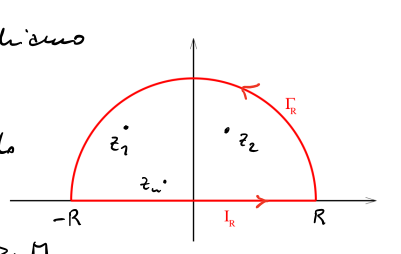
\includegraphics[width=0.5\linewidth]{images/analisi_complessa/residui_figura_1.png}
    \caption{Integrazione lungo curva}
    \label{fig:residui_1}
  \end{figure}
  Quindi otteniamo 
  \begin{equation*}
    2 \pi i \sum_{i=1}^{n} \Res_{z_i}(f) = \int_{I_R} f(z)\ dz + \int_{\Gamma_R}
    f(z)\ dz
  \end{equation*}
  il secondo integrale osserviamo che 
  \begin{equation*}
    \left|\int_{\Gamma_R} f(z)\ dz \right| \le
    \frac{K}{R^{1+a}}\mathcal{H}^{1}(\Gamma_R) = \frac{\pi K}{R^{a}}
  \end{equation*}
  e quindi tende a $0$ per $R \to +\infty$. Mentre il primo integrale
  corrisponde all'integrale improprio che volevamo calcolare. Da cui
  \begin{equation*}
     \int_{-\infty}^{+\infty} f(x)\ dx = 2\pi i \sum_{i=1}^{n} \Res_{z_i}(f)
  \end{equation*}  
\end{proof}

\begin{proposition}[Caso II]
	\label{prop:caso-ii}
    Sia $\morphism{f}{\R}{\R}$ una funzione reale continua, resitrizione di una
    funzione complessa $g \in \mathcal{O}(\Omega \setminus \left\{ z_1, \cdots,
    z_n\right\}$ e con $\Omega \supset \left\{ z \in \C \,\middle|\, \Im(z) \ge
    0\right\}$ e $z_1, \cdots, z_n \in \left\{ z \in \C \,\middle|\, \Im(z)
    > 0 \right\}$. Se esistono $K,M > 0$ tali che 
    \begin{equation*}
      |f(z)| \le \frac{K}{|z|}
    \end{equation*}
    allora vale 
    \begin{equation*}
      \int_{-\infty}^{+\infty} f(x) e^{ix} \ dx = 2\pi i \sum_{i=1}^n
      \Res_{z_i}(f(z) e^{iz})  
    \end{equation*}
\end{proposition}
\begin{proof}
    Essenzialmente ci ritroviamo a usare il Teorema dei Residui in modo analogo
    al caso I, solo che questa volta considereremo un quadrato dato che abbiamo
    anche la parte complessa della funzione $f$. Infatti possiamo riscrivere
    l'integrale come segue:
    \begin{equation*}
      \int_{-\infty}^{+\infty} f(x) e^{ix}\ dx = \int_{-\infty}^{+\infty}
      f(x)\cos(x) \ dx + i\int_{-\infty}^{+\infty} f(x)\sin(x)\ dx
    \end{equation*}
    Integriamo lungo il quadrato $\Gamma_{A,B}$ descritto in 
    Figura \ref{fig:residui_funz_fourier}
    
    \begin{figure}[h]
      \centering
      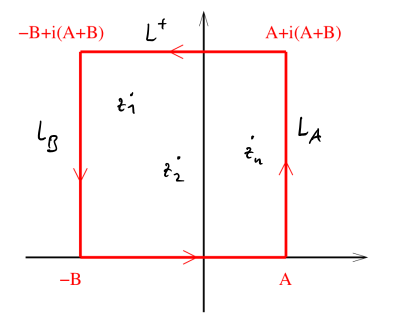
\includegraphics[width=0.4\linewidth]{images/analisi_complessa/residui_figura_2.png}
      \caption{Visualizzazione delle curve di integrazione}
      \label{fig:residui_funz_fourier}
    \end{figure}

    Spezziamo quindi l'integrazione sul quadrato nei suoi quattro lati,
    e mostriamo che l'integrale su $L_B, L_A, L^+$ tendono a $0$ per $A,B \to
    +\infty$. Scegliamo $A,B \ge M$, in maniera tale da poter poi limitare la
    funzione $f$. Prendiamo quindi il caso di $L^+$ che parametriziamo con la 
    curva $\gamma^+(x) = -x + i(A+B)$. Allora
    \begin{align*}
      \left| \int_{\gamma^+} f(z)e^{iz}\ dz  \right| & = \left| \int_{-A}^B f(-x
      + i(A+B)) (-e^{-ix - (A+B)})\ dx\right| \\
        & \le \frac{K}{T}e^{-(A+B)} \mathcal{H}^1(\gamma^+) = Ke^{-(A+B)}
    \end{align*}
    l'ultima disuguaglianza dipende dal fatto che $|f(z)| \le K/(A+B)$ per $|z| \ge
    (A+B) \ge M$. \\

    Consideriamo ora il caso del lato $L_A$, parametrizzato dalla curva
    $\gamma_A(y) = A + iy$, allora
    \begin{equation*}
      \left|\int_{\gamma_A} f(z) e^{iz}\right| 
      = \left|\int_{0}^{A+B} f(A+iy)e^{-y + iA}i \ dy \right| 
      \le \frac{K}{A} \int_{0}^{A+B} e^{-y}\ dy
    \end{equation*}
    e questo ovviamente tende a $0$ per $A+B \to +\infty$.\\
    Quindi per il Teorema dei Residui
    \begin{equation*}
      2 \pi i \sum_{i=1}^n \Res_{z_i} (f) = \int_{\Gamma_{A,B}} f(z)e^{iz}\ dz 
    \end{equation*}
    e il membro di destra ha come solo sopravvissuto 
    \begin{equation*}
      \int_{\Gamma_{A,B}} f(z)e^{iz}\ dz = \int_{A}^{B} f(z)e^{iz}\ dz \quad\
      \text{per}\ A+B \to 0
    \end{equation*}
    da cui vale la tesi.
\end{proof}

\begin{proposition}[Caso III]
  
  \begin{figure}[h]
    \centering
    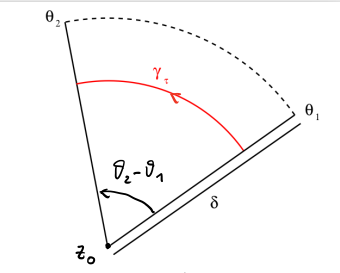
\includegraphics[width=0.4\linewidth]{images/analisi_complessa/residui_figura_3.png}
    \caption{Descrizione delle ipotesi della Proposizione \ref{prop:caso-iii}}
  \end{figure}

  Sia $\Omega$ aperto e $z_0 \in \Omega$ e $f \in
  \mathcal{O}(\Omega\setminus\left\{ z_0 \right\})$. Sia
  $\overline{B_{z_0}}(\delta) \subset \Omega$ e sia $\gamma_\tau$ l'arco di
  raggio $\tau$ con $\theta_1 \le \operatorname{arg}(\gamma_\tau) \le \theta_2$
  e $\tau \le \delta$. Se $f$ ha un polo semplice o una singolarità eliminabile
  in $z_0$ allora vale
  \begin{equation*}
    \lim_{\tau \to 0} \int_{\gamma_{\tau}} f(z) \ dz = ib(\theta_2-\theta_1)
  \end{equation*}
  \label{prop:caso-iii}
\end{proposition}
\begin{proof}
  Possiamo riscrivere 
  \begin{equation*}
    f(z) = \frac{b}{z-z_0} + h(z)
  \end{equation*}
  con $h$ olomorfa in un intorno di $z_0$. Quindi
  \begin{equation*}
    \int_{\gamma_\tau} f(z)\ dz = \int_{\theta_1}^{\theta_2}
    \frac{b}{\tau e^{i\theta}} i \tau e^{i\theta} \ d\theta + \int_{\gamma_\tau}
    h(z)\ dz
  \end{equation*}
  per cui mostriamo che il secondo integrale converge a $0$ in modulo, ovvero
  \begin{equation*}
    \left| \int_{\gamma_\tau} h(z)\ dz \right| \le \max_{\gamma_\tau} |h|
    \mathcal{H}^1(\gamma_\tau) 
  \end{equation*}
  ma la lunghezza di $\gamma_\tau\to 0$ per $\tau \to 0$, quindi tutto
  l'integrale tende a $0$.
  Per cui
  \begin{equation*}
    \lim_{\tau\to 0} \int_{\gamma_\tau} f(z)\ dz = \lim_{\tau \to 0} 
    \int_{\theta_1}^{\theta_2} \frac{b}{\tau e^{i\theta}} i \tau e^{i\theta}
    \ d\theta \to ib(\theta_2 - \theta_1) 
  \end{equation*}
\end{proof}

\begin{proposition}[Caso IV - Funzioni razionali]
  \label{prop:caso-iv}
  Siano $g,h$ polinomi reali in $x,y$ con $h \neq 0$ per $x^2 + y^2 = 1$. Allora
  possiamo definire la funzione razionale 
  \begin{equation*}
    Q(x,y) \coloneqq \frac{g(x,y)}{h(x,y)} 
  \end{equation*}
  e vale la seguente formula
  \begin{equation*}
    \int_0^{2\pi} Q(\cos(\theta), \sin(\theta)) \ d\theta = 2\pi
    i \sum_{i=1}^n \Res_{z_i} (f)
  \end{equation*}
  dove 
  \begin{equation*}
    f(z) \coloneqq \frac{1}{iz} Q\left( \frac{z+z^{-1}}{2},
    \frac{z-z^{-1}}{2i} \right)
  \end{equation*}
\end{proposition}
\begin{proof}
  Consideriamo il cerchio centrato nell'origine e di raggio $1$, parametrizzato
  dalla curva $\gamma = \partial B_0(1) = e^{i\theta}$ (con $\theta \in \left[
  0,2\pi \right]$). Allora
  \begin{equation*} 
    f(e^{i\theta}) = \frac{1}{ie^{i\theta}}
    Q\left(\cos(\theta),\sin(\theta)\right)
  \end{equation*}
  e quindi 
  \begin{equation*}
    \int_{\gamma} f(z) \ dz = \int_{0}^{2\pi} Q(\cos(\theta), \sin(\theta))\
    d\theta
  \end{equation*}
  e infine per il Teorema dei Residui si ottiene la tesi.
\end{proof}

\begin{example}\
  \begin{enumerate}
    \item Calcoliamo 
      \begin{equation*}
        I = \int_{0}^{+\infty} \frac{1}{(1+x^2)^2}\ dx = \int_{0}^{+\infty}
        f(x)\ dx
      \end{equation*}
      possiamo vedere che la funzione è pari, quindi 
      \begin{equation*}
        2I = \int_{-\infty}^{+\infty} \frac{1}{(1+x^2)^2}\ dx
      \end{equation*}
      inoltre mostriamo che $f(z)$ è limitata. Quindi 
      \begin{equation*}
        |f(z)| = \left|\frac{z^{-4}}{(z^{-2}+1)^2}\right|
        = \frac{|z|^{-4}}{|z^{-2}+1|^2} \le \frac{1}{z^{4}(1-M^2)^2}
      \end{equation*}
      con $|z| \ge M > 1$. Quindi la funzione è limitata a infinito. Calcoliamo
      infine i residui di $f$ in $\pm i$, ma solo uno dei poli sta nel
      semispazio $\Im(i) > 0$. Quindi dalla formula
      \eqref{eq:integrale_improprio_no_poli_reali} risulta
      \begin{equation*}
        2I = 2\pi i \Res_{i}(f) = 2\pi i \frac{1}{4i} = \frac{\pi}{2}
      \end{equation*}
    \item Proviamo a calcolare 
      \begin{equation*}
        I = \int_{-\infty}^{+\infty} \frac{\cos(x)}{1+x^2}\ dx  
      \end{equation*}
      definiamo $f(z) = 1/(1+z^2)$ allora questa risulta limitata in modulo
      a infinito. Inoltre possiamo vedere che l'integrale $I$ è 
      \begin{equation*}
        I = \Re\left( \int_{-\infty}^{+\infty} \frac{e^{ix}}{1+x^2} \ dx\right)
      \end{equation*}
      ovvero possiamo riscrivere per quanto visto nella Proposizione \ref{prop:caso-ii} che 
      \begin{equation*}
        I = \Re\left( 2\pi i \Res_{i} \left(\frac{e^{iz}}{1+z^2} \right) \right)
      \end{equation*}
      e poiché il residuo è $e^{-1}/2i$ si ottiene 
      \begin{equation*}
        I = \Re\left( \pi e^{-1} \right) = \frac{\pi}{e}
      \end{equation*}
    \item Calcoliamo l'integrale seguente 
      \begin{equation*}
        I = \int_{-\infty}^{+\infty} \frac{\sin(x)}{x}\ dx
      \end{equation*}
      Allora possiamo vedere che ha una singolarità in $0$, definiamo $f(z)
      = 1/z$ e la curva $\Gamma$ come in figura 
      \begin{figure}[h]
        \centering
        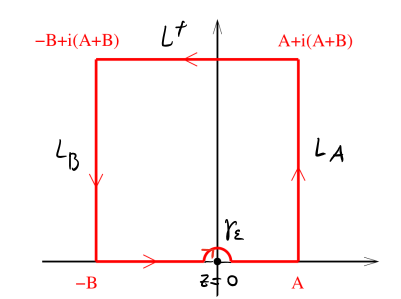
\includegraphics[width=0.4\linewidth]{images/analisi_complessa/residui_figura_4.png}
        \caption{Visualizzazione della curva $\Gamma$}
      \end{figure}
      Allora possiamo risolvere come nel caso II ma dobbiamo spezzare
      l'integrale in $3$ curve:
      \begin{equation*}
        \int_{-\infty}^{-\varepsilon} \frac{e^{ix}}{x}\ dx +
        \int_{\gamma_\varepsilon} \frac{e^{iz}}{z}\ dz +
        \int^{+\infty}_{+\varepsilon} \frac{e^{ix}}{x}\ dx
        \overset{\text{Thr. Cauchy}}{=} 0
      \end{equation*}
      per ogni $\varepsilon > 0$, ma preso sufficientemente piccolo. Per la
      Proposizione \ref{prop:caso-iii} prendiamo $\theta_1 = \pi$ e $\theta_2 = 0$ e $b
      = \Res_{0}(e^{iz}f(z)) = 1$. Allora abbiamo che per $\varepsilon \to 0$
      \begin{equation*}
        \int_{\gamma_\varepsilon} \frac{e^{iz}}{z}\ dz = - \pi i
      \end{equation*}
      e di conseguenza abbiamo che 
      \begin{equation*}
        \int_{-\infty}^{-\varepsilon} \frac{e^{ix}}{x}\ dx
        + \int_{\varepsilon}^{+\infty} \frac{e^{ix}}{x}\ dx = \pi i
      \end{equation*}
      per $\varepsilon \to 0$. Quindi 
      \begin{equation*}
        I = \Im\left( \int_{-\infty}^{+\infty} \frac{e^{ix}}{x}\ dx \right)
        = \Im(\pi i ) = \pi
      \end{equation*}
    \item Proviamo a calcolare invece l'integrale 
      \begin{equation*}
        I = \int_{0}^{2\pi} \frac{d\theta}{3-\cos(\theta)}
      \end{equation*}
      Possiamo vederlo come un integrale di un polinomio composto con $\cos,
      \sin$, quindi $Q(x,y) = 1/(3-x)$. Allora per la Proposizione
      \ref{prop:caso-iv}
      \begin{equation*}
        f(z) = \frac{1}{iz} \frac{1}{3 - \frac{z+z^{-1}}{2}}
        = \frac{1}{z-3+2\sqrt{2}} \frac{2i}{z-3-2\sqrt{2}}
      \end{equation*}
      Quindi calcoliamo solo il residuo in $z_1 = 3-2\sqrt{2}$, 
      dato che è l'unica singolarità che è all'interno di $B_0(1)$. Per cui
      \begin{equation*}
        \Res_{z_1}(f) = \frac{i}{2\sqrt{2}}
      \end{equation*}
      e quindi si ottiene 
      \begin{equation*}
        I = 2\pi i \left( -\frac{i}{2\sqrt{2}} \right) = \frac{\pi}{\sqrt{2}}
      \end{equation*}
  \end{enumerate}
\end{example}

%todos: 0

\def \ord {\operatorname{ord}}

\chapter{Zeri di funzioni olomorfe}

Lo scopo principale di questo capitolo è di dimostrare il \emph{Principio di
indentità}, ovvero se due funzioni olomorfe coincidono in un qualche intorno di
un punto, allora sono identiche.

\begin{theorem}
   \label{thr:zeri_di_funz_no_accum}
  Sia $\Omega \subset \C$ aperto connesso e $f\in \mathcal{O}(\Omega)$ non
  identicamente nulla e sia $Z(f) \coloneqq \left\{ z \in \Omega \,\middle|\,
  f(z) = 0 \right\}$. Allora  $Z(f)$ non ha punti di accumulazione in $\Omega$.
  (Gli zeri di una funzione olomorfa sono isolati).
\end{theorem}
\begin{proof}
    Dimostriamo la tesi a livello locale. Per cui prendiamo $z_0 \in Z(f)$. Se
    $f$ non è identicamente nulla in un intorno di $z_0$, segue che $z_0$ è uno
    zero di molteplicità $m > 0$ quindi in un intorno di $z_0$ la serie di
    Laurent di $f$ prende forma
    \begin{equation*}
      f(z) = (z-z_0)^m g(z)
    \end{equation*}
    con $g$ olomorfa in un intorno di $z_0$ e $g(z_0) \neq 0$.
    Restringendo opportunamente l'intorno si può trovare un nuovo intorno tale
    per cui $g \neq 0$. Segue che anche $f(z) \neq 0$ se $z \neq z_0$, per cui
    lo zero $z_0$ è uno zero isolato di $f$.\\

    Per ottenere il risultato globale usiamo la proprietà di connessione di
    $\Omega$. Infatti sia $A \subset \Omega$ l'insieme dei punti di
    accumulazione di $Z(f)$ in $\Omega$. Noi sappiamo che $f$ è continua, quindi
    dev'essere che $A \subset Z(f)$ (infatti se $z$ fosse di accumulazione
      e $f(z) \neq 0$ allora vorrebbe dire che esiste una sequenza di $\{s_n\}
    \subset Z(f)$ tale che $f(s_n) = 0$ e che $s_n \to z$, ma con 
    $\lim_{n\to+\infty} f(s_n) \neq f(z)$ per cui $f$ non sarebbe continua).
    % TODO: chiarire meglio questa parte.
    \begin{enumerate}
    	\item Se $A$ è aperto allora $z_0 \in A$ quindi è uno zero isolato
    	di $f$ e per quanto visto sopra possiamo trovare un intorno in cui $f \neq
    	0$ per tutto un intorno escluso $z_0$. Quindi l'intorno dovrebbe essere
    	contenuto in $A$, ma ciò vorrebbe dire che $A \not\subset Z(f)$. 
    	\item Se $A$ chiuso allora esiste una sequenza $z_n \to z$ con $z_n \in A$ e che
    	convergono ancora in $z \in A$. In particolare se $z \in Z(f)$ allora $z$
    	non sarebbe isolato (e abbiamo visto che non è il caso) quindi $z \in A$
    	e quindi $A \not\subset Z(f)$.
    \end{enumerate}
  Pertanto dev'essere che $A = \varnothing$.
\end{proof}

\begin{corollary}[Principio di Identità]
    \label{cor:principio_indentita}
  Sia $\Omega \subset \C$ aperto connesso e $f,g \in \mathcal{O}(\Omega)$. Se
  esiste $S \subset \Omega$ tale che $f|_S = g|_S$ e $S$ ha punti di
  accumulazione in $\Omega$ allora $f = g$ in $\Omega$.
\end{corollary}
\begin{proof}
  Sia $h = f - g$, osserviamo che la differenza di funzioni olomorfe su $\Omega$
  sarà ancora olomorfa. Allora per il Teorema \ref{thr:zeri_di_funz_no_accum},
  sapendo che $S \subseteq Z(h)$, abbiamo che l'insieme $Z(h)$ ha almeno
  un punto di accumulazione in $\Omega$ (per Bolzano-Weierstrass), pertanto si
  conclude che $h$ è la funzione identicamente nulla su tutto $\Omega$.
\end{proof}

% TODO: portare la definizione di meromorfa, qui, perché dov'era non aveva
% senso. Era stata introdotta e lasciata a marcire, quindi mettiamola dove può
% servire effettivamente la sua definizione.
\begin{corollary}
	\label{thr:rapporto_olomorfe_diventa_meromorfa}
  Sia $\Omega \supset \C$ connesso e $f,g \in \mathcal{O}(\Omega)$ con $f \neq
  0$ allora $g / f \in \mathcal{M}(\Omega)$ 
\end{corollary}
\begin{proof}
  Sia $S$ l'insieme degli zeri di $f$. Questi sono punti isolati e sono poli 
  di $1/f$. Quindi $g/f$ è olomorfa in $\Omega \setminus S$ con $S$ insieme 
  discreto di $\Omega$ da cui dalla definizione di funzione meromorfa si 
  ottiene la tesi.
\end{proof}

\begin{definition}
\label{def:ordine_funz_meromorfa}
  Sia $f\in \mathcal{M}(\Omega)$ e $z_0 \in \Omega$. Se $a_m$ è il primo
  coefficiente non nullo della serie di Laurent di $f$ centrata in $z_0$, allora 
  \begin{equation*}
    \ord_{z_0} (f)  \coloneqq m
  \end{equation*}
  si dice \textbf{ordine di $f$ in $z_0$}.
\end{definition}

\begin{remark}
  Osserviamo per prima cosa che $\ord_{z_0}(f) \in \Z$. Se l'ordine è positivo
  allora coincide con l'ordine dello zero in $z_0$ di $f$; se l'ordine
  è negativo, invece corrisponde all'ordine cambiato di segno dell'ordine del
  polo in $z_0$.  
  \label{rmk:insight_ordine}
\end{remark}

\begin{theorem}[Principio dell'argomento]
	\label{thr:principio_dell_argomento}
  Sia $f \in \mathcal{M}(\Omega)$ con un numero finito di zeri e poli $z_1,
  \cdots, z_n \in \Omega$. Sia $\gamma$ catena in $\Omega$ e $\gamma \sim_\Omega
  0$ con $\image(\gamma) \cap \left\{ z_1, \cdots, z_n\right\} = \varnothing$.
  Allora 
  \begin{equation*}
    \int_{\gamma} \frac{f'(z)}{f(z)}\ dz = 2\pi i \sum_{i=1}^{n}
    \Ind_\gamma(z_i) \ord_{z_i}(f)
  \end{equation*}
\end{theorem}
\begin{proof}
  Mostriamo che $f'/ f \in \mathcal{O}(\Omega')$ dove $\Omega' \coloneqq \Omega
  \setminus \left\{ z_1, \cdots, z_n \right\}$ e $f'/f \in \mathcal{M}(\Omega)$
  e con ordine $\ord_{z_i}(f) = \Res_{z_i}(f'/f)$.
  Infatti $f(z) \neq 0$ su $\Omega'$ e allora segue che è olomorfa su tutto
  $\Omega'$. Inoltre visto che ha un numero finito di singolarità isolate
  è meromorfa su $\Omega$. Nell'intorno di $z_i$ possiamo decomporre $f$ secondo
  la serie di Laurent
  \begin{equation*}
    f(z) = (z-z_i)^{m_i}h(z) 
  \end{equation*}
  con $m_i = \ord_{z_i}(f)$ per definizione e $h$ funzione olomorfa tale che
  $h(z_i) \neq 0$. Quindi derivando $f$ si ottiene 
  \begin{equation*}
    f'(z) = m_i(z-z_i)^{m_i-1}h(z) + (z-z_i)^{m_i}h(z)
  \end{equation*}
  per ogni $z \neq z_i$ vicino a $z_i$. Segue quindi che 
  \begin{equation*}
    \frac{f'(z)}{f(z)} = \frac{m_i}{z-z_i} + \frac{h'(z)}{h(z)}
  \end{equation*}
  con $h'/h$ funzione olomorfa in un intorno di $z_i$. Si può concludere che
  $m_i = \Res_{z_i}(f'/f)$. La formula segue quindi dal Teorema dei Residui \ref{} 
  % TODO aggiungere riferimento al teorema dei Residui.
\end{proof}

\begin{corollary}
  Sia $\Omega \subset \C$ aperto, $f \in \mathcal{M}(\Omega)$. Sia $\gamma$ una
  curva di Jordan in $\Omega$ e la parte interna deve stare in $\Omega$
  e l'immagine di $\gamma$ non si intersechi con zeri o poli di $f$. Indicando
  con $N_0$ il numero di zeri di $f$ contenuti all'interno di $\gamma$, 
  contati con la loro molteplicità; $N_\infty$ il numero di poli di $f$
  contenuti all'interno di $\gamma$, contati con il loro ordine. Allora vale la
  seguente formula
  \begin{equation*}
    \frac{1}{2 \pi i} \int_{\gamma} \frac{f'(z)}{f(z)}\ dz = N_0 - N_\infty
  \end{equation*}
  \label{cor:principio_id_per_curve_semplici}
\end{corollary}
\begin{proof}
  Dato che $\gamma \sim_\Omega 0$ per deduzione dalle ipotesi
  e $\Ind_{\gamma}(z_i) = 1$ per ogni zero o polo (visto che si trova nella
  parte interna di una curva di Jordan), allora se indichiamo con $S_1$
  l'insieme degli zeri di $f$ nell'interno di $\gamma$ e con $S_2$ l'insieme
  dei poli all'interno di $\gamma$, allora  
  \begin{equation*}
    N_0 = \sum_{z_i \in S_1} \ord_{z_i}(f) \quad\ N_\infty = - \sum_{z_i \in
    S_2} \ord_{z_i}(f)
  \end{equation*}
  allora dal Teorema del Principio dell'Argomento
  \ref{thr:principio_dell_argomento} segue la tesi.
\end{proof}

\begin{corollary}
  Se $f \in \mathcal{M}(\C)$ e l'interno di una curva di Jordan $\gamma$
  contiene tutti gli zerie i poli di $f$ allora
  \begin{equation*}
    N_0 - N_\infty = - \Res_\infty\left( \frac{f'}{f} \right)
  \end{equation*}
  \label{cor:residuo_infinito_rispetto_all_ordine}
\end{corollary}
\begin{proof}
  Segue dalla definizione di $\Res_\infty(f'/f)$ e dal Corollario
  \ref{cor:principio_id_per_curve_semplici}.
\end{proof}

\begin{remark}
  Il \emph{Principio dell'argomento} deriva dall'interpretazione geometrica
  dell'integrale \begin{equation*}
    \frac{1}{2\pi i} \int_{\gamma} \frac{f'(z)}{f(z)}\ dz
  \end{equation*}
  come \emph{variazione dell'argomento} dei punti della curva $f \circ \gamma$.
  Ad esempio si consideri 
  \begin{equation*}
    f(z) = \frac{1}{z^2} \quad\ \gamma(t) = e^{it} 
  \end{equation*}
  allora $f \circ \gamma(t) = e^{-2it}$ ovvero percorre una circonferenza in
  senso orario due volte. Si ha quindi 
  \begin{equation*}
    \frac{1}{2\pi i} \int_{\gamma} \frac{f'(z)}{f(z)}\ dz
    = \frac{1}{2\pi i} \int_{\gamma} \frac{-2}{z}\ dz = -2
  \end{equation*}
  e la variazione $\Delta_{f \circ \gamma} \operatorname{arg}(w)$ dell'argomento
  di $w = f \circ \gamma(t)$ lungo la curva $f \circ \gamma$ è $-4\pi$ (ovvero
  la lunghezza della curva, orientata). Quindi vale 
  \begin{equation*}
    \frac{1}{2\pi i} \int_{\gamma} \frac{f'}{f}\ dz = \frac{1}{2\pi}
    \Delta_{f\circ \gamma}\operatorname{arg}(w)
  \end{equation*}

  In generale se $g$ è una funzione logaritmo di $f$, cioè $e^{g} = f$ con $f,g$
  funzioni olomorfe, si ha 
  \begin{equation*}
    f' = (e^g)' = e^g g' = fg'
  \end{equation*}
  ovvero $g' = f'/f$. Osserviamo infine che la derivata logaritmica di $f$ non
  dipende dalla branca del logaritmo di $g$, infatti si ha 
  \begin{align*}
    \int_{\gamma} \frac{f'}{f}\ dz & = \int_{\gamma} (\log(f))' \ dz
    = \log(f(\gamma(b))) - \log(f(\gamma(a)))\\
    & = \ln |f(\gamma(b))| - \ln |f(\gamma(a))|
    + i(\operatorname{arg}(f(\gamma(b))) - \operatorname{arg}(f(\gamma(a)))) \\
    & = i \Delta_{f \circ \gamma} \operatorname{arg}(w)
  \end{align*}
  per cui 
  \begin{equation*}
    \frac{1}{2\pi i} \int_{\gamma} \frac{f'}{f}\ dz = \frac{1}{2\pi i}
    \Delta_{f\circ \gamma}\operatorname{arg}(w) = \Ind_{f\circ \gamma}(0)
  \end{equation*}
  \label{rmk:motivazione_principio_argomento}
\end{remark}

\begin{theorem}[Teorema di Rouché]
   \label{thr:rouche}
  Sia $\Omega \subset \C$ aperto e $f,g \in \mathcal{O}(\Omega)$ e $\gamma$
  curva di Jordan in $\Omega$ con interno contenuto in $\Omega$. Se vale 
  \begin{equation}
    \label{eq:rouche_stima_ipotesi}
    |f(z) - g(z)| < |f(z)|
  \end{equation}
  allora $f$ e $g$ non hanno zeri in $\image(\gamma)$ e hanno lo stesso numero
  di zeri (contati con molteplicità) nell'interno di $\gamma$.
 
\end{theorem}
\begin{proof}
  Per ipotesi $f,g$ non si annullano su $\gamma$:
  Supponiamo che esiste $z \in \gamma$ tale che $f(z) = 0$ allora per
  \eqref{eq:rouche_stima_ipotesi} valrebbe che 
  \begin{equation*}
    |g(z)| < 0
  \end{equation*}
  che è impossibile. Se $g(z) = 0$ allora si avrebbe ancora per
  \eqref{eq:rouche_stima_ipotesi}
  \begin{equation*}
    |f(z)| < |f(z)|
  \end{equation*}
  da cui è ancora assurdo. Segue che $f,g$ non si annullino su $\gamma$.\\

  Sia $h = g/f$, questa è una funzione meromorfa su $\Omega$. Osserviamo che $h
  \circ \gamma$ ha supporto all'interno della palla in $1$ di raggio $1$, ovvero
  $\image(h \circ \gamma) \subset B_1(1)$, poiché 
  \begin{equation*}
    |h(z) - 1| = \frac{|f(z) - g(z)|}{|f(z)|} < 1
  \end{equation*}
  dove $z = \gamma(t)$ per qualche $t$. In particolare osserviamo che
  $\Ind_{h\circ \gamma}(0) = 0$ poiché $0 \notin B_1(1)$. Ovvero appartiene
  all'esterno del supporto della curva $h \circ \gamma$. Quindi
  \begin{equation*}
    0 = 2\pi i \Ind_{h\circ \gamma}(0) = \int_{h \circ \gamma}
    \frac{dw}{w} = \int_{a}^b \frac{h'(\gamma(t))\gamma'(t)}{h(\gamma(t))}\ dt
    = \int_{\gamma} \frac{h'(z)}{h(z)}\ dz
  \end{equation*}
  Infine osservando che 
  \begin{equation*}
    \frac{h'}{h} = \frac{g'f - gf'}{f^2} \frac{f}{g} = \frac{g'}{g}
    - \frac{f'}{f}
  \end{equation*}
  allora segue che 
  \begin{equation*}
    \int_{\gamma} \frac{g'(z)}{g(z)}\ dz = \int_{\gamma} \frac{f'(z)}{f(z)}\ dz
  \end{equation*}
  Per il Corollario \ref{cor:residuo_infinito_rispetto_all_ordine} i due
  integrali sono uguali, così come i residui e quindi anche lo stesso numero di
  zeri contati con molteplicità.
\end{proof}

\begin{example}
  Presentiamo qui alcuni esempi per trovare, per confronto (e utilizzo del
  Teorema di Rouché \ref{thr:rouche}), gli zeri di una funzione. In questo caso
  particolare nel caso di funzioni polinomiale. Ma per le proprietà locali ogni
  funzione olomorfa può ossere approssimata ad una serie di Laurent e quindi
  è equivalente a trovare gli zeri di un polinomio.
  \begin{enumerate}
    \item Prendiamo $p(z) = z^8 - 5z^3 + z -2$ e $f(z) = -5z^3$. Sulla
      circonferenza $|z| = 1$ vale 
      \begin{equation*}
        |p(z) - f(z)| = |z^8 + z -2| \le |z|^8 + |z| + 2 = 4 < 5|z|^3 = |f(z)|
      \end{equation*}
      quindi $p$ ha $3$ zeri tanti quanti come $f$ nel disco unitario $|z| < 1$
      e non si annulla per $|z| =1$. Scegliamo ora $g(z) = z^8$ si controlliamo
      nella circonferenza $|z| = 2$, 
      \begin{equation*}
        |p(z) - g(z)| \le 5|z|^3 + |z| + 2 \le 44 < |g(z)|
      \end{equation*}
      quindi si può concludere che $p$ ha tutti i suoi $8$ zeri in $|z| < 2$, in
      particolare ne ha $5$ nella corona circolare di raggi $1$ e $2$.
    \item Consideriamo $q(z) = 4z^5 - z^3 + z^2 -2$, analogamente a quanto fatto
      nell'esempio precedente per controllare dove sono locati tutti gli zeri
      possiamo confrontarlo con la funzione $f(z) = 4z^5$ sulla circonferenza di
      raggio $B_0(1+\varepsilon)$. Allora
      \begin{equation*}
        |q(z) - f(z)| \le |z|^3 + |z|^2 - 2 < |f(z)|
      \end{equation*}
      dunque per ogni $\varepsilon > 0$ $q$ ha $5$ zeri in $B_0(1+\varepsilon)$.
      Per cui possiamo concludere per l'arbitrarietà di $\varepsilon$ che tutti
      gli zeri di $q(z)$ si trovano in $\overline{B_0(1)}$.
  \end{enumerate}
\end{example}

\section{Principio del Massimo Modulo}

Per ottenere i seguenti teoremi: \emph{Principio del Massimo}; il 
\emph{Teorema della mappa aperta}; il \emph{Teorema della mappa inversa}. Ci
serve un risultato sul comportamento locale delle funzioni olomorfe, che vedremo
essere analogo a quello di una funzione $z^n$ per qualche $n\in \Z$.

\begin{theorem}
	\label{thr:tecnico_principio_massimo}
  Sia $\Omega \subset \C$ aperto, $f \in \mathcal{O}(\Omega)$ e $z_0 \in \Omega$
  uno zero di ordine $m$ di $f$. Esiste $\varepsilon_0 > 0$ tale che per ogni $0
  < \varepsilon < \varepsilon_0$ esiste $\delta > 0$ tale che per ogni $w_0 \in
  \C$ con $|w_0| < \delta$ l'equazione $f(z) = w_0$ ha $m$ soluzioni in
  $B_{z_0}(\varepsilon)$ distinte se $w_0 \neq 0$ (nel caso $m > 1$). 
\end{theorem}
\begin{proof}
    Sia $z_0$ uno zero isolato di $f$ allora esiste $\varepsilon_0 > 0$ tale che
    $B_{z_0}(\varepsilon_0) \subset \Omega$ e $f(z) \neq 0$ per $z \in
    B_{z_0}(\varepsilon_0) \setminus \left\{ z_0 \right\}$. Sia $0 < \varepsilon
    < \varepsilon_0$ e sia $\gamma = \partial B_{z_0}(\varepsilon)$ e poniamo 
    $\delta = \min_{z \in \gamma} |f(z)| > 0$. Se $|w_0| < \delta$ allora $g
    = f - w_0$ è una funzione olomorfa su tutto $\Omega$ e vale 
    \begin{equation*}
      |f(z) - g(z)| = |w_0| < \delta \le |f(z)| \quad\ \forall z \in
      \image(\gamma)
    \end{equation*}
    
    Utiliziamo il Teorema di Rouché \ref{thr:rouche} su $g$. Allora $g$ ha $m$
    zeri in $B_{z_0}(\varepsilon)$ che equivale a dire che $f(z) = w_0$ ha $m$
    soluzioni (con molteplicità) nella palla $B_{z_0}(\varepsilon)$.
    Se $m = 1$ si ha la tesi.
    Se $m > 1$ allora $z_0$ è uno zero anche di $f'$ che avrà uno zero di ordine
    $m-1$. Se $\varepsilon_0$ viene scelto sufficientemente piccolo in modo che
    $Z(f') \cap B_{z_0}(\varepsilon_0) = \left\{ z_0 \right\}$ si ha che $g'
    \neq 0$ su $B_{z_0}(\varepsilon) \setminus \left\{ z_0 \right\}$ ovvero gli
    zeri di $g$ sono tutti semplici. Ovvero le soluzioni di $f(z) = w_0$ ono
    tutte distinte per $w_0 \neq 0$.
\end{proof}

\begin{corollary}
	\label{cor:tecnico_principio_massimo}
  Sia $f \in \mathcal{O}(\Omega)$ non costante e $z_0 \in \Omega$. Sia $f(z_0)
  = \alpha$ e $\ord_{z_0}(f-\alpha) = m$. Allora esiste $\varepsilon_0 > 0$ tale
  che per ogni $0 < \varepsilon < \varepsilon_0$ esiste un $\delta > 0$ tale che
  per ogni $w_0$ con $|w_0 - \alpha| < \delta$, l'equazione $f(z) = w_0$ ha $m$
  soluzioni in $B_{z_0}(\varepsilon)$ distinte se $w_0 \neq \alpha$.
\end{corollary}
\begin{proof}
  Si usa il Teorema precedente \ref{thr:tecnico_principio_massimo} a $f - \alpha
  \in \mathcal{O}(\Omega)$.
\end{proof}

\begin{theorem}[Teorema Della Mappa Aperta]
  \label{thr:mappa_aperta}
  Sia $\Omega \subset \C$ aperto connesso e $f \in \mathcal{O}(\Omega)$ non
  costante. Allora $f$ è una mappa aperta.
\end{theorem}
\begin{proof}
  Sia $A \subset \Omega$ aperto e $\alpha = f(z_0)$ per qualche $z_0 \in A$.
  Allora esiste $B_{z_0}(\varepsilon) \subset A$ tale che $f - \alpha \neq 0$ in
  $B_{z_0}(\varepsilon) \setminus \left\{ z_0 \right\}$. Se $\varepsilon
  < \varepsilon_0$ come nel Corollario precedente, allora esiste $\delta > 0$
  tale che $|w_0 - \alpha| < \delta$ e allora $w_0 \in f\left(
  B_{z_0}(\varepsilon) \right) \subset f(A)$. Cioè $B_{\alpha}(\delta) \subset
  f(A)$ per ogni $\alpha \in f(A)$ dato che non abbiamo imposto alcuna ipotesi
  su $\alpha$. Pertanto $f(A)$ è intorno di ogni suo punto ed è aperto. 
\end{proof}

\begin{theorem}[Principio Del Massimo]
  \label{thr:principio_del_massimo}
  Sia $\Omega \subset \C$ aperto e connesso e $f \in \mathcal{O}(\Omega)$ non
  costante. Allora $|f|$ non ha massimi locali in $\Omega$. 
\end{theorem}
\begin{proof}
  Sappiamo che $f$ è aperta per Teorema della Mappa Aperta
  \ref{thr:mappa_aperta}. Allora per ogni $\alpha = f(z_0) \in \image(f)$ e per
  ogni intorno $B_{z_0}(\varepsilon)$ di $z_0$ essendo
  $f \left(B_{z_0}(\varepsilon) \right)$ aperto contenente $\alpha$ allora esiste
  un'altra palla aperta $B_\alpha(\delta) \subset f\left( B_{z_0}(\varepsilon) 
  \right)$. In particolare esistono degli $f(z) \in f\left( B_{z_0}(\varepsilon
  \right) \setminus B_\alpha(\delta)$, per cui dev'essere che 
  \begin{equation*}
    |f(z)| > |\alpha| = |f(z_0)|
  \end{equation*}
  con $|z-z_0| < \varepsilon$. Quindi segue che $z_0$ non può essere un punto
  di massimo locale. Poiché $z_0$ è stato scelto in modo arbitrario questa
  conclusione vale per ogni punto $z_0 \in \Omega$.
\end{proof}

\begin{corollary}
  \label{cor:massimo_sul_bordo}
  Sia $\Omega$ aperto connesso con chiusura $\overline{\Omega}$ compatto. Se $f
  \in \mathcal{O}(\Omega) \cap C^0(\overline{\Omega})$ allora
  \begin{equation*}
    \max_{\overline{\Omega}} |f| = \max_{\partial \Omega} |f|
  \end{equation*}
\end{corollary}
\begin{proof}
  Dato che sussiste il Principio del massimo \ref{thr:principio_del_massimo},
  allora dev'essere che $f$ non ha un massimo nella parte interna, dev'essere
  sul bordo, poiché $|f|$ è continua e per Weierstrass deve avere massimo. 
\end{proof}

\begin{theorem}[Teorema della mappa inversa]
	  \label{thr:mappa_inversa}
  Sia $f \in \mathcal{O}(\Omega)$ con $z_0 \in \Omega$ con $f'(z_0) \neq 0$.
  Esiste un intorno aperto $V$ di $z_0$ e un intorno aperto $W$ di $f(z_0)$
  tali che $\morphism{f}{V}{W}$ è invertibile con inversa
  $\morphism{f^{-1}}{W}{V}$ olomorfa. Vale inoltre la formula
  \begin{equation*}
    (f^{-1})'(w) = \frac{1}{f'(f^{-1}(w))}
  \end{equation*}
  per ogni $w \in W$.
\end{theorem}
\begin{proof}
  Poniamo $\alpha = f(z_0)$. La funzione $g(z) = f(z) - \alpha$ è una funzione
  olomorfa con uno zero di molteplicità $1$ in $z_0$. Infatti $g'(z_0) = f'(z_0)
  \neq 0$. Per il Corollario \ref{cor:tecnico_principio_massimo} esistono
  $\varepsilon, \delta > 0$ tali che l'equazione $f(z) = w_0$ per ogni $w_0 \in
  B_\alpha(\delta)$ ha un unica soluzione in $B_{z_0}(\varepsilon)$. Per cui
  basta porre $V = B_{z_0}(\varepsilon)$ e $W = B_\alpha(\delta)$ e si vede che 
  $\morphism{f}{V}{W}$ è una mappa biunivoca e olomorfa; in più risulta essere
  una mappa aperta per il Teorema della mappa Aperta \ref{thr:mappa_aperta}.
  Quindi $f^{-1}$ dev'essere una funzione continua. Osserviamo anche che $f'(z)
  \neq 0$ per ogni $z\in V$, dato che se no la funzione non sarebbe biunivoca.

  Mostriamo che $f^{-1}$ è olomorfa su $W$. Siano $z_1 = f^{-1}(w_1)$ e $z_2
  = f^{-1}(w_2)$. Si ha per continuità che 
  \begin{equation*}
    \lim_{w \to w_1} \frac{f^{-1}(w) - f^{-1}(w_1)}{w-w_1} = \lim_{z \to z_1}
    \frac{z-z_1}{f(z)- f(z_1)} = \frac{1}{f'(z_1)} = \frac{1}{f'(f^{-1}(w_1)}
  \end{equation*}
  e il limite esiste per ogni punto $w_1 \in W$.
\end{proof}

\begin{remark}
  Se $f'(z_0) = 0$, la funzione $f$ non è iniettiva, in quanto $z_0$ è uno zero
  di $g = f - f(z_0)$ di ordine $m > 1$. Nell'intorno di $z_0$ l'equazione $f(z)
  = w_0$ ha $m > 1$ soluzioni, quindi $f$ non è invertibile. Sui reali invece
  questo non è vero, per esempio $f(x) = x^3$.
  \label{rmk:complessi_limitano_le_inverse}
\end{remark}

%todos: 0

\chapter{Mappe conformi}
Un importante risultato dell'analisi complessa riguarda le mappe conformi: sono utilizzate spesso perché permettono - grazie alla loro proprietà del preservare localmente gli angoli - di mantenere inalterate alcune proprietà dello spazio di partenza mappandole in uno spazio di arrivo più comodo.
\newpage
\section{Una mappa che preserva gli angoli}
\subsection{\textcolor{AnComp}{\textbf{Il significato geometrico delle mappe conformi}}}

Come abbiamo visto, una conseguenza delle equazioni di Cauchy-Riemann soddisfatte dalle componenti
reali di una funzione olomorfa è 

\begin{corollary}
  La matrice Jacobiana della funzione reale $\morphism{(u,v)}{\Omega \subset
  \R^2}{\R^2}$ è
  \begin{equation*}
    J_f = \left(\begin{array}{cc} 
        u_x & -v_x\\
        v_x & u_x
    \end{array}\right) 
  \end{equation*}
  se inoltre $\morphism{f}{\C}{\C}$ e tale che $f = u + iv$ è una funzione
  olomorfa allora vale che
  \begin{equation*}
    \det J_f = u^2_x + v^2_x = |f'(z)|^2 \ge 0 
  \end{equation*}
\end{corollary}

\begin{remark}
  La proprietà descritta nel Corollario precedente descrive mappe che hanno un 
  senso geometrico molto importante. Infatti se $f'(z_0) \neq 0$, vuol dire che
  la mappa preserva gli angoli. Se vale questa proprietà, si dice che una mappa
  è \textbf{conforme} in $z_0$.
  \label{rmk:conforme_intuizione}
\end{remark}
\subsection{\textcolor{AnComp}{\textbf{Le mappe conformi come funzioni olomorfe}}}
\begin{theorem}
 \label{thr:conferme_sse_jacobiana_non_nulla}
  Sia $\morphism{f}{\Omega}{\C}$ e $z_0 \in \Omega$. Sia $f = u + iv$ con $u,v$
  differenziabili in $z_0$. Allora $f$ è conforme in $z_0$ se e solo se esiste
  la derivata complessa di $f'(z_0)$ e vale che $f'(z_0) \neq 0$.
\end{theorem}
\begin{proof}\
  \begin{enumerate}
    \item[$\Rightarrow$] Se $f$ è differenziabile in $z_0$ allora $J_f(z_0) = 
      |f'(z_0)|^2 > 0$ per ipotesi. Sia quindi $(u_x,v_x) = (r\cos\theta, 
      r\sin\theta)$ con 
      \begin{equation*}
        r = \sqrt{u_x^2 + v_x^2} = |f'(z_0)|^2 > 0 
      \end{equation*}
      allora la matrice Jacobiana di $f$ in $z_0$ diventa
      \begin{equation*}
        \left(\begin{array}{cc}
          r & 0 \\
          0 & r
      \end{array}\right)
       \left( \begin{array}{cc}
          \cos\theta & - \sin \theta \\
          \sin \theta & \cos \theta
      \end{array}\right)
      \end{equation*}
      corrisponde alla composizione di una rotazione con una omotetia, ma sono
      entrambe trasformazioni che preservano gli angoli, da cui la tesi.
    \item[$\Leftarrow$] Sia $f$ conforme in $z_0$. Sia $\theta$ l'angolo tra
      i vettori $(1,0)$ e $J(1,0)$ con $J = J_f(z_0)$. Per cui costruiamo una
      rotazione $R_\theta$ tale che $R_\theta^{-1}(J(1,0)) = (r,0)$ con $r > 0$
      dato che se no $f$ non preserverebbe gli angoli. In particolare chiediamo
      $R^{-1}_\theta$ una rotazione che rende l'angolo tra $(1,0)$
      e $R^{-1}_\theta(J(1,0))$ sia nullo. Segue che la
      trasformazione $G = R^{-1}_\theta J$ preserva gli angoli. Quindi segue che
      anche $G (0,1) = (0, s)$ con $s > 0$.  Per cui $G(1,1) = (r,s)$
      e dev'essere che $r = s$ dato che se non preserverebbe gli angoli. Per cui
      consideriamo $(a,b)$ vettore qualsiasi, vale che $G(a,b) = r(a,b)$.
      Because algebra: 
      \begin{equation*}
        R^{-1}_\theta J = I_r \Longrightarrow J = J_f(z_0) = R_\theta I_r
      \end{equation*}
      scritto in termini matriciali diventa
      \begin{equation*}
        J_f(z_0) = \left( 
          \begin{array}{cc}
          u_x & u_y \\
          v_x & v_y 
          \end{array}\right) = 
          \left( 
            \begin{array}{cc}
              r\cos\theta & -r\sin\theta \\
              r\sin\theta & r\cos\theta 
            \end{array}
          \right)
      \end{equation*}
      da cui segue subito che $u_x = v_y$ e $u_y = - v_x$, ovvero soddisfa le
      condizioni di Cauchy-Riemann. Pertanto $f$ è differenziabile e inoltre
      vale che $f'(z_0) \neq 0$ dato che $J \neq 0$.
  \end{enumerate}
\end{proof}

\begin{corollary}
  Una funzione $f$ complessa è conforme in $\Omega$ se e solo se $f \in
  \mathcal{O}(\Omega)$ e $f'(z) \neq 0$ per ogni $z \in \Omega$. 
  \label{cor:estensione_teorema_conformita}
\end{corollary}

\begin{definition}
  Si dice che $\morphism{g}{\Omega}{\C}$ è una funzione \textbf{antiolomorfa} se
  esiste $\morphism{f}{\Omega}{\C}$ funzione olomorfa su $\Omega$ tale che
  $\overline{g} = f$.
  \label{def:antiolomorfa}
\end{definition}

\begin{remark}
  Se si richiede che $f$ conservi solo l'ampiezza dell'angolo e non
  l'orientazione, allora anche le funzioni antiolomorfe giocano un ruolo.
  Infatti se una funzione $g$ è antiolomorfa si ha che $J_g \le 0$ e chiedendo
  che $J_g \neq 0$ si ottiene una mappa che non modifica l'ampiezza degli
  angoli, ma ne inverte l'orientazione.  
  \label{rmk:anticonformita}
\end{remark}

\begin{remark}
  La mappa $f$ è conforme in $z_0$ se e solo se per ogni coppia di vettori non
  nulli $a,b \in \R^2$, l'angolo in $z_0$ tra due curve $\gamma_a, \gamma_b$ con
  $\gamma_a(0) = \gamma_b(0) = z_0$ e $\gamma'_(0) = a$, $\gamma'_b(0) = b$
  è uguale all'angolo in $f(z_0)$ e le curve $f \circ \gamma_a, f \circ
  \gamma_b$. \\

  \begin{figure}[h]
    \centering
    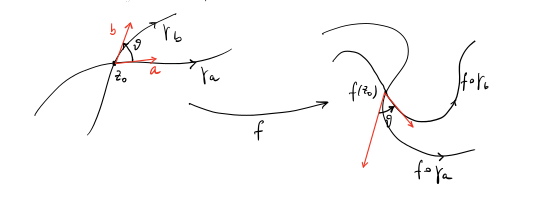
\includegraphics[width=0.6\linewidth]{images/analisi_complessa/es_mappa_conforme1.png}
    \caption{Rappresentazione della condizione di mantenimento dell'angolo tra
    due curve}
    \label{fig:mappe_conformi_1}
  \end{figure}

  Infatti se $f = u+iv$ e $\gamma_a(t) = (x(t), y(t))$, si ha 
  \begin{equation*}
    (f\circ \gamma_a)' = (u_x x' + u_y y') + i(v_x x' + v_y y')
  \end{equation*}
  e quindi vale 
  \begin{equation}
    \label{eq:globglob}
    (f\circ \gamma_a)'(0) = \left(\begin{array}{cc}
        u_x & u_y \\
        v_x & v_y 
    \end{array}\right) 
        \left(\begin{array}{c}
            x'(0) \\
            y'(0) 
        \end{array}\right) = J_f(z_0)a
  \end{equation}
  $(f\circ \gamma_a)'(0) = J_f(z_0) a$ e analogamente vale
  $(f\circ \gamma_b)'(0) = J_f(z_0) b$. Per cui dato che l'angolo viene 
  preservato, segue che $J_f(z_0) > 0$ e $f$ risulta essere conforme in $z_0$.\\

  Analogamente se $f$ è conforme abbiamo che $J_f(z_0) \neq 0$ e vale comunque
  l'identità \eqref{eq:globglob}, da cui si ha che 
  \begin{align*}
    \gamma'_a(0) = a & \parallel (f \circ \gamma_a)'(0) = J_f(z_0) a\\
    \gamma'_b(0) = b & \parallel (f \circ \gamma_b)'(0) = J_f(z_0) b
  \end{align*}
\end{remark}

\begin{example}\
  \begin{enumerate}
    \item Sia $f(z) = z^2$ allora possiamo osservare che $f'(z) \neq 0$ per $z
      \neq 0$. Quindi $f$ risulta essere conforme in $\C \setminus \left\{ 0
      \right\}$.
      \begin{figure}[h]
        \centering
        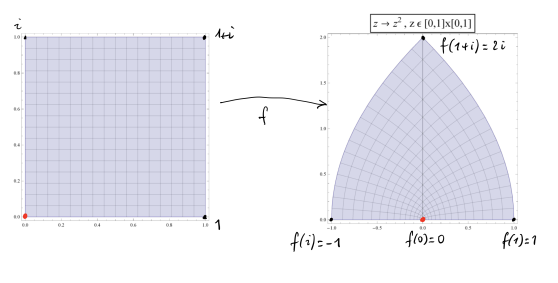
\includegraphics[width=0.6\linewidth]{images/analisi_complessa/es_mappa_conforme2.png}
        \caption{Visualizzazione di come vengono mantenuti gli angoli al di
        fuori del punto $0$}
        \label{fig:mappe_conformi_esempio1}
      \end{figure}
    \item Sia $f(z) = z^3$ anche questa è tale che $f'(z) \neq 0$ per ogni $z
      \neq 0$.
    \item Sia $f(z) = e^z$, questa risulta essere conforme su tutto $\C$ dato
      che $f'(z) = e^z$ e ha modulo sempre positivo. 
      \begin{figure}[h]
        \centering
        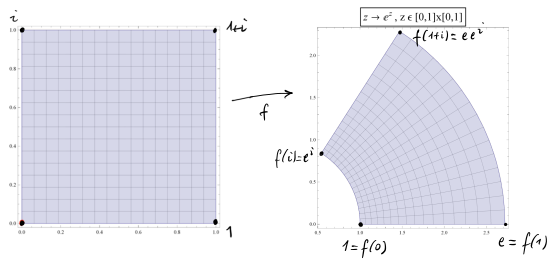
\includegraphics[width=0.6\linewidth]{images/analisi_complessa/es_mappa_conforme4.png}
        \caption{Visualizzazione della mappa $e^z$ conforme su tutto $\C$}
        \label{fig:mappe_conformi_esempio3}
      \end{figure}
    \item Sia invece
      \begin{equation*}
        f(z) = \frac{z^2 - i}{z^2 + i} 
      \end{equation*}
      questa risulta essere conforme su 
      \begin{equation*}
        \C \setminus \left\{ 0, \frac{\sqrt{2}}{2} - \frac{\sqrt{2}}{2}i,
        -\frac{\sqrt{2}}{2} + \frac{\sqrt{2}}{2}i \right\}
      \end{equation*}
      In particolare è conforme su tutto il primo e terzo quadrante.

      \begin{figure}[h]
        \centering
        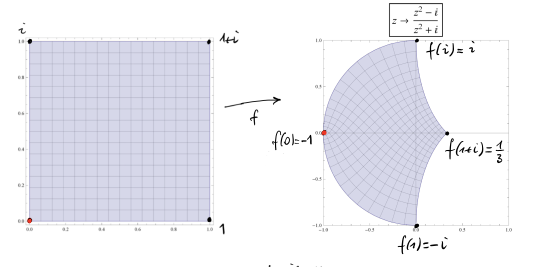
\includegraphics[width=0.6\linewidth]{images/analisi_complessa/es_mappa_conforme5.png}
        \caption{Visualizzazione di $f$ sul primo quadrante}
        \label{fig:mappe_conformi_esempio4}
      \end{figure}
  \end{enumerate}
\end{example}

%todos: 0


\chapter{Estensione di funzioni in $\C$}
Come ci si può aspettare, alcune funzioni notevoli dell'analisi reale avranno uno spazio dedicato alla costruzione delle rispettive estensioni complesse. Non sempre sarà facile come ci si potrebbe aspettare, e faremo del nostro meglio per far capire come sia importante soffermarsi a ragionare su alcuni dettagli che spesso trascuriamo essendo abituati a \enquote{ragionare in $\mathbb{R}$}. \\ \\ Ad esempio: $\operatorname{log}(a^n)=n \ \operatorname{log}(a)$\dots \textit{chi l'ha deciso?}
\newpage
\section{Funzione esponenziale}
\subsection{\textcolor{AnComp}{\textbf{La funzione esponenziale}}}
\begin{definition}
	\label{defn:funzione-esponenziale}
	Definiamo l'esponenziale in $\C$ come la serie di potenze
	\begin{equation*}
		e^z := \sum^{+\infty}_{k=0} \frac{z^k}{k!}
	\end{equation*}
\end{definition}

Possiamo osservarne alcune caratteristiche fondamentali. 

\begin{theorem}
	La funzione esponenziale gode delle seguenti proprietà:
	\begin{enumerate}
		\item è olomorfa in $\C$
		\item $(e^z)' = e^z$
		\item $e^{i\theta} = \cos \theta + i\sin \theta$ per $\theta \in \R$
		\item è periodica di periodo $2\pi i$
		\item $e^z \neq 0$ per ogni $z \in \C$ (in particolare non è biunivoca)
	\end{enumerate}
\end{theorem}
\begin{proof} \
	\begin{enumerate}
		\item Per definizione e per il Teorema \ref{thr:teorema-di-abel}.
		\item Dal calcolo esplicito della derivata della serie di potenze:
		$$\begin{aligned} (e^z)' & = \sum^{+\infty}_{n=1} n\frac{z^{n-1}}{n!} = \sum^{+\infty}_{n=1} \frac{z^{n-1}}{(n-1)!} \\
		& = \sum^{+\infty}_{p=0} \frac{z^p}{p!} = e^z \end{aligned}$$
		\item Anche per questo basta un calcolo esplicito: \begin{equation*}
		\begin{aligned}
		e^{iz} & = \sum^{+\infty}_{n=0} \frac{(iz)^{n}}{n!} = \sum^{+\infty}_{k=0} \frac{(iz)^{2k}}{2k!} + \sum^{+\infty}_{k=0} \frac{(iz)^{2k+1}}{2k+1!}\\
		& = \sum^{+\infty}_{k=0} (-1)^k\frac{z^{2k}}{2k!} + i\sum^{+\infty}_{k=0} (-1)^k\frac{z^{2k+1}}{2k+1!}\\
		& = \cos z + i \sin z
		\end{aligned}
		\end{equation*}
		\item Basta osservare che $e^{a + 2\pi i} = e^a e^{2\pi i } = e^a$, il fatto che $e^{2\pi i} = 1$ è naturale dal punto precedente.
		\item 	Sia $\alpha \in \C$, allora $e^z = \alpha$ vuol dire che se $z = x+iy$ allora 
		\begin{equation*}
		\begin{cases}
		x = \ln |\alpha|\\
		y = \arg \alpha
		\end{cases}
		\end{equation*}
		per cui se $\alpha = 0$, $x$ non sarebbe ben definito. Mentre per tutti gli altri valore di $\alpha \in \C$ è definita.
		
	\end{enumerate}
\end{proof}

\subsection{\textcolor{AnComp}{\textbf{Le funzioni trigonometriche}}}
	
	\begin{definition}
		\label{defn:sin-cos}
		Definiamo le funzioni trigonometriche in funzione delle serie di potenze come segue:
		\begin{equation*}
			\sin(z) := \sum^{+\infty}_{k=0} (-1)^k\frac{z^{2k+1}}{(2k+1)!} \;\ \cos(z) := \sum^{+\infty}_{k=0} (-1)^k\frac{z^{2k}}{(2k)!}
		\end{equation*}
	\end{definition}
	
	\begin{theorem}
		Valgono le seguenti proprietà delle funzioni trigonometriche:
		\begin{enumerate}
			\item 
			\begin{equation*}
			\begin{aligned}
				\sin(z) = \frac{e^{iz} - e^{-iz}}{2i} \;\ \cos(z) = \frac{e^{iz} + e^{-iz}}{2}
			\end{aligned}
			\end{equation*}
			\item sono $2\pi$ periodiche
			\item non sono limitate
			\item l'immagine di $\sin$ e $\cos$ coincide con $\C$
			\item le seguenti funzioni sono olomorfe dovunque nel piano complesso meno che nei loro rispettivi poli
			\begin{equation*}
			\begin{aligned}
				\tan z & := \frac{\sin z}{\cos z} \in \mathcal{O}(\C \setminus \{ \pi /2 + k\pi \mid k \in \N \}) \\
				\cot z & := \frac{\cos z}{\sin z} \in \mathcal{O}(\C \setminus \{k\pi \mid k \in \N \})
			\end{aligned}
			\end{equation*}
		\end{enumerate}
	\end{theorem}
	\begin{proof}\ 
		%TODO: proof  (G)
		%ne ho messe un paio ma sono troppo stanco per finirle (S)
	\begin{enumerate}
		\item Per algebra:
			\begin{align*}
				\sin(z) & = \frac{e^{iz} - e^{-iz}}{2i} = \frac{1}{2i} \sum_{j=0}^{+\infty} \frac{(iz)^{j}}{j!} - \frac{(-iz)^{j}}{j!} \\
					 	& = \frac{1}{2i} \sum_{j=0}^{+\infty} \frac{(iz)^j - (-iz)^j}{j!}
			\end{align*}
			Dobbiamo vedere i diversi casi per cui $i^{4k} = 1$, $i^{4k + 1} = i$, $i^{4k + 2} = -1$, $i^{4k + 3} = -i$. A questo punto abbbiamo tre sommatorie rispettivamente 
			\begin{align*}
				\frac{1}{2i} \sum_{j=0}^{+\infty} \frac{(iz)^{4j} - (-iz)^{4j}}{4j!} & = 0 \\
				\frac{1}{2i} \sum_{j=0}^{+\infty} \frac{(iz)^{4j+1} - (-iz)^{4j+1}}{(4j+1)!} & = \frac{1}{2i} \sum_{j=0}^{+\infty} i\frac{z^{4j+1}}{(4j+1)!} \\
				\frac{1}{2i} \sum_{j=0}^{+\infty} \frac{(iz)^{4j+2} - (-iz)^{4j+2}}{(4j+2)!} & = 0 \\
				\frac{1}{2i} \sum_{j=0}^{+\infty} \frac{(iz)^{4j+3} - (-iz)^{4j+3}}{(4j+3)!} & = \frac{1}{2i} \sum_{j=0}^{+\infty} -i\frac{z^{4j+3}}{(4j+3)!} \\
			\end{align*}
			da cui si trova la stessa definizione di $\sin(z)$ con $z \in \C$.
		\item Osserviamo che l'esponziale complesso $e^{iz}$ con $z \in \C$, allora se $z = a + ib$ vale che $e^{ia - b}$ che è $2\pi$ periodico in funzione della parte reale di $z$. Analogamente per $e^{-iz}$, questo dà la ben conosciuta proprietà di $2\pi$ periodicità sull'asse reale delle funzioni trigonometriche.
		\item Supponiamo per assurdo che siano limitate. Sappiamo che $\sin(z), \cos(z)$ sono funzioni intere, ovvero sono olomorfe su tutto $\C$ (deriva dal fatto che si possono scrivere come combianzione lineare di funzioni intere). Allora per il Teorema di Liouville dev'essere che $\sin(z), \cos(z)$ siano costanti. Ma è ovvio che non lo sono, infatti basta calcolarsi due valori e vedere che non lo sono i.e. si prenda $z = \pi$ e $z = \pi/2$. Pertanto abbiamo una contraddizione. Segue che $\sin(z), \cos(z)$ non possono essere limitate.  
		\item Sia $y \in \C$ allora vale che $y = \sin(z)$ sse esiste una soluzione a 
		\begin{equation*}
			2cw = w^2 + 1 \quad\ \text{con}\ w = e^{iz}
		\end{equation*} 
		e questa esiste per ogni $c$ da cui la tesi.
		\item Basta osservare che il coseno ha zeri in $\pi/2 k$ con $k \in \Z$, per vederlo si può usare Rouché o più banalmente basta far vedere che se la parte immaginaria $>0$ allora $\cos(z) > 0$.    
	\end{enumerate}
	\end{proof}
	
\subsection{\textcolor{AnComp}{\textbf{Il logaritmo ed il logaritmo principale}}}
	
	\begin{definition}
		\label{defn:logaritmo-principale}
		Il \textbf{logaritmo principale} è la funzione definita come:
		\begin{align*}
		& \morphism{\log}{\C \setminus \{x \in \R \mid x \le 0\}}{\C} \\
		\log(z) = & \ln(|z|) + i\arg z \ \text{  con  } \ \arg z \in (-\pi,\pi]
		\end{align*}
		
	\end{definition}

	\begin{remark}
		In generale si perdono molte delle proprietà del logaritmo che valevano in $\R$. Per esempio $\log(xy) \neq \log(x)+\log(y)$.
	\end{remark}

	\begin{theorem}
		La funzione logaritmo principale è olomorfa e la sua derivata è 
		\begin{equation*}
			\log'(z) = 1/z
		\end{equation*}
	\end{theorem}
	\begin{proof} \
		Dimostriamo che è olomorfa grazie alle equazioni di Cauchy-Riemann, per cui ponendo
		\begin{equation*}
		\begin{aligned}
			\log(x+iy) = \frac{1}{2}\ln(x^2 + y^2) + i\arctan(y/x) = u(x,y) + iv(x,y)
		\end{aligned}
		\end{equation*}
		da cui le derivate ci danno le relazioni cercate.\\
		
		Sempre utilizzando le equazioni di Cauchy-Riemann otteniamo al tesi, cioè che $\log'(z) = u_x + iv_x = 1/z$.
	\end{proof}
	\begin{remark}
		Osserviamo infine che la funzione argomento può prendere valori con periodicità di $2\pi$, perciò abbiamo effettivamente infinite definizioni della funzione logaritmo. \\ Questo può presentare alcuni vantaggi. Infatti la funzione radice quadrata principalmente è 
		$f_0(z) = e^{\log(z)/2} = \sqrt{|z|}e^{i(\arg z)/2}$, ma se si usa un'altra definizione di logaritmo, ovvero consideriamo una diversa possibile branca (o determinazione) della radice quadrata, otteniamo $f_1(z) = e^{\log'(z)/2} = \sqrt{|z|}e^{i\arg(z)/2 + i\pi}$, che rappresenta la \textit{radice ``negativa''}. 
	\end{remark}

%todos: 0



% --- APPENDIX & BACKMATTER ------------------------------------

\appendix
% 1. Rifare la teoria con il retratto di deformazione forte vs debole
% 2. Insiemistica di base
%\include{}

% TODO? bibliografia
%\backmatter
%    Bibliography styles amsplain or harvard are also acceptable.
\bibliographystyle{amsalpha}
\begin{thebibliography}{9}
	\bibitem{riehl-cat-theory} 
		Emily Riehl,
		\textit{Category Theory in Context},
		\url{http://www.math.jhu.edu/~eriehl/context.pdf}
\end{thebibliography}
%    See note above about multiple indexes.

\end{document}
